\documentclass[a4paper,12pt]{report}

\usepackage{fontspec}
\usepackage{polyglossia}
\setmainlanguage{hungarian}
\usepackage[a4paper,margin=2.4cm]{geometry}
\usepackage{graphicx}
\usepackage{float}
\usepackage{hyperref}
\usepackage{amsmath}
\usepackage{amssymb}
\usepackage{booktabs}
\usepackage{array}
\usepackage{tabularx}
\usepackage{longtable}
\usepackage{caption}
\usepackage{enumitem}
\usepackage{listings}
\usepackage{xcolor}
\usepackage{titlesec}
\usepackage{url}

\titleformat{\chapter}[hang]{\normalfont\bfseries\LARGE}{\thechapter.}{1em}{}
\setcounter{tocdepth}{2}
\setlist[itemize]{noitemsep, topsep=4pt}
\setlength{\parskip}{0.5em}
\setlength{\parindent}{0pt}
\graphicspath{{assets/demo_shots/}{assets/diagrams/}}
\setmainfont{Times New Roman}
\setsansfont{Arial}
\setmonofont{Consolas}

\lstset{
  basicstyle=\ttfamily\small,
  breaklines=true,
  frame=single,
  columns=fullflexible,
  keepspaces=true
}

\newcommand{\diagramfigure}[2]{
\begin{figure}[H]
\centering
\includegraphics[width=0.92\textwidth]{#2}
\caption{#1}
\end{figure}
}

\newcommand{\placeholder}[2]{%
\begin{figure}[H]
\centering
\fbox{\parbox{0.85\textwidth}{\centering\vspace{2.2cm}%
\textbf{[PLACEHOLDER]}\par\vspace{0.4em}{\small #1}\vspace{2.2cm}}}%
\caption{#2}
\end{figure}%
}

\begin{document}

\begin{titlepage}
    \centering
    {\LARGE UMFST \par}
    \vspace{1.2cm}
    {\Large Informatikai Kar \par}
    \vspace{3.3cm}
    {\huge\bfseries Premade Graph Explorer\par}
    \vspace{0.5cm}
    {\Large League of Legends játékoskapcsolatok, teljesítménymutatók és gráfanalitikai kiterjesztések\par}
    \vfill
    {\Large Készítette: Tamási Krisztián-Erik\par}
    \vspace{2.3cm}
    {\large Marosvásárhely, 2026\par}
\end{titlepage}

\tableofcontents
\clearpage

\part{PremadeGraph rendszer és gráfanalitika}

% ===== chapters/01-bevezetes.tex =====
\chapter{Bevezetés}

\section{Problémafelvetés}

A kompetitív online játékok egyik visszatérő problémája, hogy a résztvevők nagyon erős véleményeket fogalmaznak meg egymás teljesítményéről, miközben ehhez rendszerint csak részleges, szubjektív és rövid távú benyomások állnak rendelkezésre. Egy elveszített mérkőzés után gyorsan megjelenik a bűnbakkeresés, de sokkal ritkábban történik meg az, hogy a játékosok valóban adatalapon próbálják megérteni, mi történt a meccsben, hogyan teljesítettek ők maguk, és hogyan helyezhető el ez a teljesítmény egy tágabb közösségi hálózatban.

A \emph{League of Legends} különösen érdekes terep ehhez, mert egyszerre tartalmaz rendkívül gazdag mérkőzésadatokat, ismétlődő csapattársi és ellenfél-kapcsolatokat, valamint olyan társas mintázatokat, amelyek gráfként ábrázolhatók és elemezhetők. Ha egy játékos hosszabb időn keresztül ugyanazokkal az emberekkel kerül egy meccsbe -- akár szövetségesként, akár ellenfélként --, akkor ebből egy olyan kapcsolati háló építhető fel, amely túlmutat az egyetlen mérkőzés pillanatnyi statisztikáin.

Ebből a felismerésből indult a dolgozat: nem egyszerűen egy újabb meccsnéző vagy statisztikai felületet akartam készíteni, hanem egy olyan rendszert, amely a valós mérkőzéstörténetből játékoshálót épít, ezt a hálót gráfelméleti és rendszerszintű szemlélettel elemzi, majd az eredményeket egy vizuálisan erős, ugyanakkor védhető frontend felületen mutatja meg.

\section{Motiváció}

A projekt eredeti motivációja személyes és technikai egyszerre. Játékosként újra és újra felmerült bennem a kérdés, hogy vajon a visszatérő negatív tapasztalatok mennyire egyediek, mennyire mintázatszerűek, és egyáltalán látszik-e valami abból a hálózatból, amelynek részeként ezek a meccsek zajlanak. Informatikai oldalról pedig kifejezetten vonzott az a gondolat, hogy a Riot API által biztosított részletes meccsadatokból nemcsak táblázatokat, hanem gráfokat, klasztereket, útvonalakat és teljesítményalapú hálózati mutatókat is lehessen kinyerni.

A projekt időközben jóval nagyobb rendszerré nőtt, mint egy egyszerű adatvizualizáció. A jelenlegi állapotban már külön adatgyűjtő réteg, normalizált pontszámítási pipeline, SQLite perzisztencia, Rust-alapú gráfépítés és futtatókörnyezet, többoldalas React frontend, valamint kutatási jellegű gráfanalitikai modulok dolgoznak együtt. A Python réteg elsősorban adatgyűjtési, prototípus- és legacy-kompatibilitási szerepben maradt meg.

\section{A dolgozat célja}

A dolgozat célja egy olyan, valós mérkőzésadatokra épülő, többkomponensű rendszer bemutatása, amely:

\begin{itemize}
    \item League of Legends meccsekből játékosok közötti kapcsolatokat gyűjt és tisztít,
    \item a játékosokhoz szerepkör-érzékeny teljesítménymutatókat rendel,
    \item az ismétlődő együtt- és egymás ellen játszásból gráfot épít,
    \item a gráfot klaszterekre, útvonalakra, core-periphery mintázatokra és kutatási célú metrikus kapcsolatokra bontja,
    \item a számításigényes részeket determinisztikus, exportálható és újrafuttatható módon kezeli,
    \item az eredményeket interaktív, de nem UI-első szemlélettel mutatja meg.
\end{itemize}

A hangsúly tudatosan azon van, hogy a rendszer ne csak érdekes látvány legyen, hanem szakdolgozati szempontból is védhető legyen: világos adatútvonalakkal, expliciten dokumentált döntésekkel, reprodukálható kimenetekkel és óvatos interpretációval.

\section{Kutatási kérdések}

A jelen dolgozatban a következő kutatási kérdésekre keresem a választ:

\begin{itemize}
    \item Hogyan építhető fel valós League of Legends mérkőzéstörténetből egy olyan játékosháló, amely nem pusztán az együtt játszást, hanem az ellenfél-kapcsolatokat is megőrzi?
    \item Milyen módon lehet a játékosok teljesítményét úgy pontozni, hogy az figyelembe vegye a tényleges szerepkört, de közben megmaradjon értelmezhetőnek?
    \item Mennyiben indokolt a rendszer különböző rétegeit Python, SQLite, Node.js, Rust és React komponensekre bontani?
    \item Mutat-e a jelenlegi gráf pozitív asszortativitást a \texttt{opscore} és \texttt{feedscore} tekintetében?
    \item Miben különbözik a \texttt{flexset} és a \texttt{soloq} kapcsolati szerkezete, és mennyiben írható le a \texttt{flexset} asszociatív core-periphery játékosgráfként?
\end{itemize}

\section{A dolgozat hozzájárulása}

A dolgozat gyakorlati és szakmai hozzájárulásai a jelenlegi implementáció alapján a következők:

\begin{itemize}
    \item több-adatkészletes, regiszter-alapú mérkőzésgyűjtési és feldolgozási architektúra;
    \item szerepkörérzékeny, adatbázis-alapú \texttt{opscore}/\texttt{feedscore} normalizáció;
    \item Rust-központú Graph V2 gráfépítés, klaszterezés és artifact-export SQLite perzisztenciával;
    \item Rust oldali útvonalkeresés BFS, Dijkstra, kétirányú keresés, egzakt A*, asszortativitás és Brandes-központisági támogatással;
    \item \texttt{flexset} és \texttt{soloq} dataset-összehasonlítás asszociatív gráfértelmezéssel;
    \item játékosteljesítményre számolt asszortativitási elemzés több gráfmódban;
    \item előre kiszámított 3D globális gráfnézet és többoldalas, kutatásbarát frontend.
\end{itemize}

\begin{figure}[H]
    \centering
    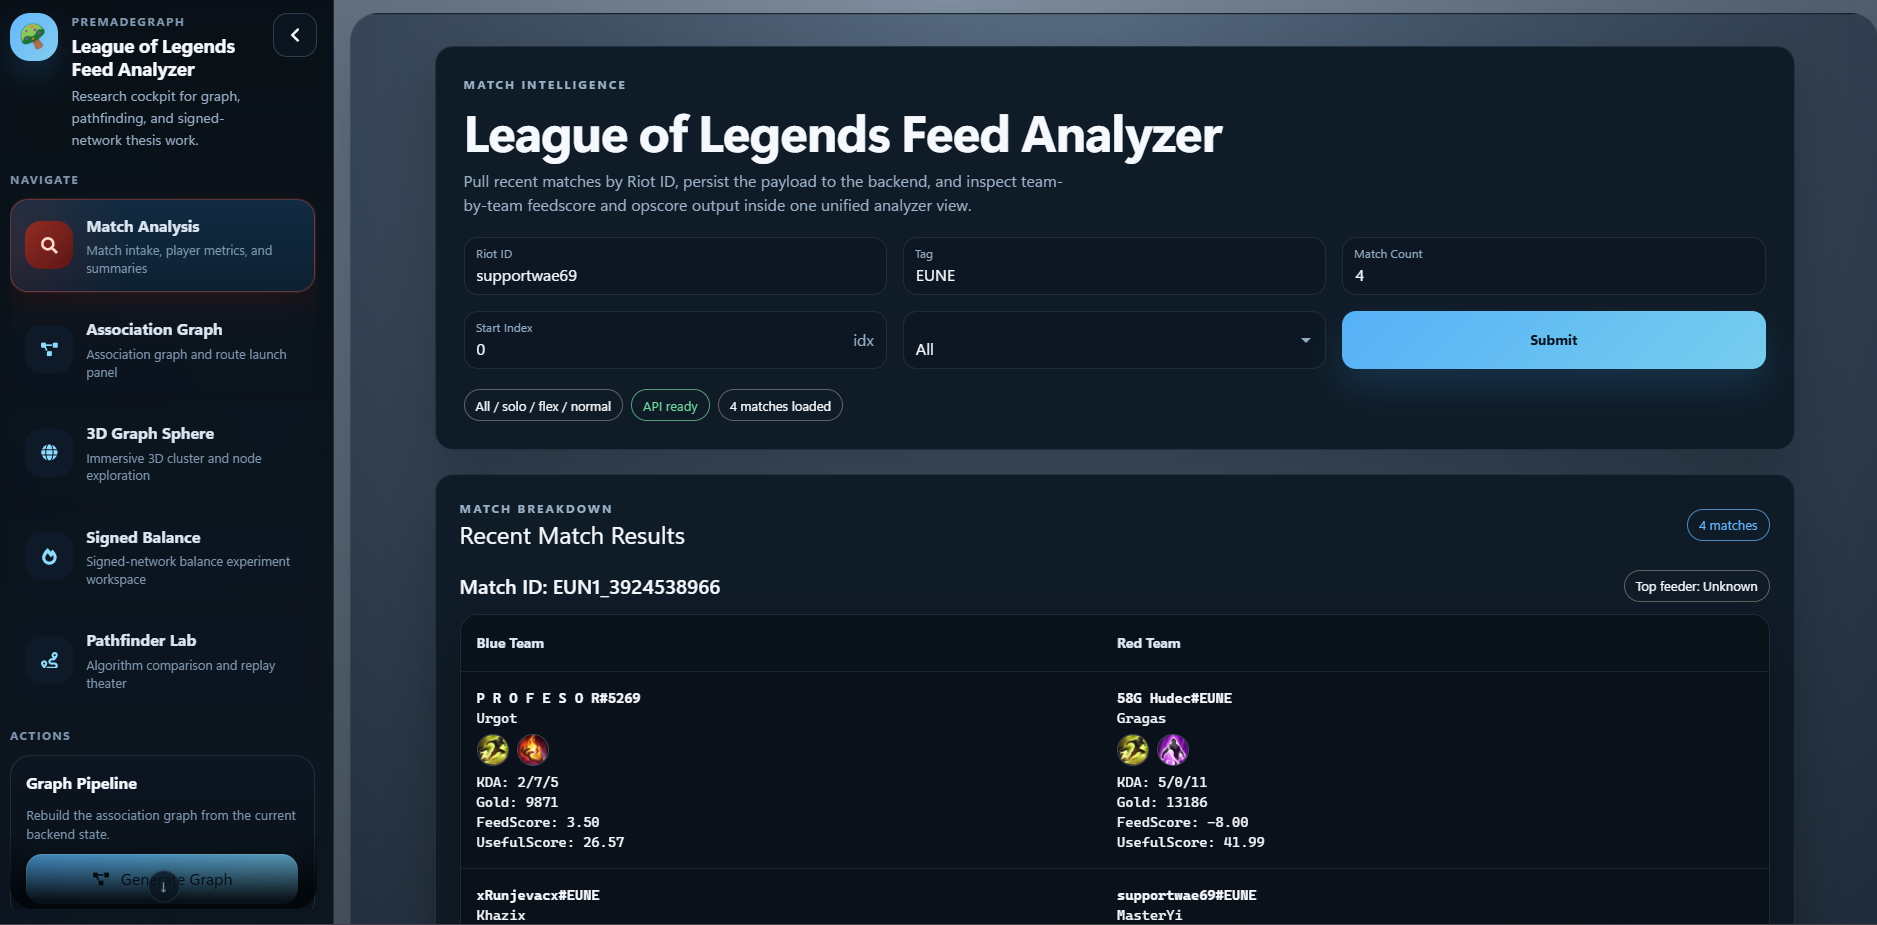
\includegraphics[width=0.92\textwidth]{match-analysis-page.png}
    \caption{A jelenlegi frontend egyik belépési pontja: meccselemzési és adatgyűjtési felület}
\end{figure}

% ===== chapters/02-problemafelvetes-es-motivacio.tex =====
\chapter{Problémafelvetés és motiváció}

\section{Miért nem elég egy hagyományos statisztikai oldal?}

A legtöbb, játékosoknak szánt statisztikai felület egyetlen mérkőzésre, egyetlen rangsorra vagy néhány alapmutatóra szűkíti le az értelmezést. Ez önmagában hasznos lehet, de nem válaszolja meg azt a kérdést, amely engem a projekt elejétől fogva érdekelt: vajon a mérkőzések mögött kirajzolódik-e egy tartós társas szerkezet, és ha igen, ez a szerkezet hogyan kapcsolódik a teljesítményhez?

Ebből a szempontból a \emph{Premade Graph} lényegében két problémát kezel egyszerre. Az első probléma adatmérnöki: hogyan lehet nyers Riot API válaszokból olyan hosszabb élettartamú adatkorpuszt felépíteni, amelyben a játékosok azonosítása, a meccsek tárolása, a pontszámítás és a gráfprojekció újrafuttatható módon történik. A második probléma kutatási: hogyan lehet ebből a korpuszból olyan állításokat megfogalmazni, amelyek nem csak látványosak, hanem meg is védhetők.

Ez az oka annak, hogy a dolgozat fókusza tudatosan nem egyetlen UI-oldal vagy egyetlen algoritmus. A projekt értéke éppen abban áll, hogy az adatgyűjtés, a tisztítás, a pontszámítás, a gráfépítés, a klaszterezés, a futásidejű analitika és a vizualizáció ugyanannak a rendszernek az egymásra épülő rétegei.

\section{A projekt szokatlan és érdekes volta}

A szakdolgozat témája azért különösen érdekes, mert a kiinduló adathalmaz nem egyszerű játékoslista, hanem ismétlődő interakciós háló. A rendszer ugyanazt a két játékost nemcsak egyszeri ellenfelekként látja, hanem potenciális visszatérő szövetségesként, visszatérő ellenfélként, klasztertagként, hídcsúcsként vagy egy nagyobb globális hálózat részeként is.

Ez több okból ad erős szakdolgozati alapot:

\begin{itemize}
    \item a League of Legends mérkőzésadatai elég gazdagok ahhoz, hogy valódi teljesítményprofilok legyenek számíthatók;
    \item a visszatérő együttjátszás és egymás elleni előfordulás gráfelméleti szempontból értelmezhető kapcsolatokat hoz létre;
    \item a szövetségesi és ellenfél-jelleg együttese miatt a projekt nem csak súlyozott, hanem többféle kapcsolatprojekcióként is vizsgálható;
    \item a rendszer implementációs oldalon is érdekes, mert több nyelv és futtatókörnyezet közötti felelősségmegosztást kell megindokolni.
\end{itemize}

Ez a kombináció ritkább, mint elsőre látszik. Sok játékelemző projekt vagy a vizuális oldalnál áll meg, vagy csak egy-egy táblázatos mutatóig jut el. Itt viszont ugyanannak a rendszernek része a nyers adatgyűjtés, a szerepkörérzékeny score-réteg, a klaszterezés, az útvonalkeresés, az asszortativitási analitika, a Brandes-központiság és a 3D globális megjelenítés.

\section{A központi szakdolgozati állítás}

A dolgozat fő tézise az, hogy \emph{a valós mérkőzéstörténetből felépített League of Legends játékosháló egyszerre kezelhető mint asszociatív játékosgráf, mint teljesítményprofilokkal dúsított adatstruktúra, és mint rendszertechnikai szempontból komoly, többnyelvű analitikai platform}. Ennek a tézisnek három pillére van.

\subsection{Hálózati pillér}

A meccsekből olyan gráf építhető, amelyben a játékosok közötti ismétlődő együttjátszás és egymás elleni előfordulás már nem véletlenszerű zajként, hanem mérhető szerkezeti mintázatként jelenik meg. A \texttt{flexset} esetében ennek legerősebb olvasata az asszociatív core-periphery szerkezet: a központi régióban hídgazdag, visszatérő ally-csoportok, a periférián pedig sok kis, gyengén kapcsolt lokális csoport jelenik meg. Ez teszi lehetővé a klaszterezést, az útvonalkeresést, az asszortativitást és a későbbi centralitási validálást.

\subsection{Metrikai pillér}

A játékosokhoz rendelhető olyan \texttt{feedscore} és \texttt{opscore}, amely nem tökéletes vagy végleges igazság, de elég értelmezhető és következetes ahhoz, hogy későbbi gráfanalitikai bemenet legyen. A szerepkörérzékeny súlyozás és a percentilis-alapú normalizáció itt nem kozmetikai döntés, hanem a teljes későbbi elemzés előfeltétele.

\subsection{Rendszertechnikai pillér}

A projekt a jelenlegi állapotában már túlmutat azon, amit egyetlen script vagy egyetlen technológia kényelmesen elbírna. A Python, az SQLite, a Node/Express, a Rust és a React együttese nem véletlen felhalmozódás, hanem olyan architekturális válasz, amely a különböző részfeladatok eltérő természetéből következik. Ezt a dolgozatban külön, döntési és kompromisszum-alapú szemlélettel fogom indokolni.

\section{Hatókör, nem-célok és őszinteségi szabályok}

A projekt mérete könnyen csábíthatna arra, hogy minden meglévő ötletet kész eredményként mutassak be. Ezt a dolgozatban tudatosan kerülöm. Három szabályt tekintek fontosnak.

\begin{itemize}
    \item Amit a kódbázisban jelenleg ténylegesen megvalósultnak és ellenőrizhetőnek találtam, azt kész állapotként írom le.
    \item Amit a repository megőriz korábbi kísérleti ágként, de a jelenlegi adatsnapshotban nincs érdemi kimenete, azt korábbi vagy kiegészítő modulként kezelem.
    \item Amit a fejlesztési dokumentáció csak jövőbeli célként fogalmaz meg, azt nem nevezem kész feature-nek.
\end{itemize}

Ennek a szabálynak különösen nagy jelentősége van a következő területeken:

\begin{itemize}
    \item a klaszterekhez kötött ország- és régióelemzés kódja megvan, de a jelenlegi ellenőrzött adatbázis-pillanatképben nem tartalmaz kitöltött országcímkéket.
\end{itemize}

\section{A dolgozat szerkezete}

A dolgozat logikája a projekt fejlődését követi. Előbb bemutatom a problémafelvetést és a szakirodalmi hátteret, majd a Riot API-ra épülő adatforrásokat és a korai pipeline-t. Ezután térek rá a pontozási rendszerre, a gráfépítésre és a régi ország-alapú elemzési ágra. A középső fejezetek az architektúra evolúcióját, a több-adatkészletes modellt, az SQLite perzisztenciát és a Rust futtatókörnyezetet tárgyalják. Végül külön fejezetekben mutatom be a Pathfinder Labot, a 3D bird's-eye sphere nézetet, az asszortativitási és központisági elemzéseket, valamint a strukturális egyensúly módszertani visszaminősítését, majd a validációt, a rendszerszintű értékelést és a jövőbeli fejlesztéseket.

% ===== chapters/03-szakirodalmi-hatter.tex =====
\chapter{Szakirodalmi háttér}

\section{Hálózatkutatás és közösségszerkezet}

A gráfok társas kapcsolatok modellezésében régóta központi szerepet játszanak. A videojátékos közösségek esetében különösen izgalmas kérdés, hogy a játékosok közötti ismétlődő interakciók mennyiben alkotnak felismerhető struktúrákat, szubközösségeket, hidakat és lokális mintázatokat. Girvan és Newman klasszikus munkája rámutatott arra, hogy a hálózat élei nem pusztán kapcsolódási elemek, hanem közösségszerkezetet leíró, eltérő fontosságú viszonyok is lehetnek \cite{girvannewman}. Fortunato átfogó áttekintése pedig jól összefoglalja, miért központi probléma a közösségdetektálás a modern hálózatelemzésben \cite{fortunato2010}.

A jelen projektben a közösségfogalom nem öncélú. Azért fontos, mert a többször ismétlődő kapcsolatokra épülő játékoscsoportok:

\begin{itemize}
    \item értelmezhetőbbé teszik a nagyméretű hálózatot,
    \item segítenek elkülöníteni a valós kapcsolati magokat a zajtól,
    \item támaszt nyújtanak a későbbi útvonal- és analitikai számításoknak.
\end{itemize}

\section{Közösségdetektálás és modularitás}

A korai Python oldali populációs klaszterezés a NetworkX \texttt{greedy\_modularity\_communities} eljárását használta, amely a Clauset--Newman--Moore féle mohó modularitásmaximalizálási megközelítésre épül \cite{clauset2004,networkx_greedy}. Ez a választás prototípusként tudatos kompromisszum volt: nem a leglátványosabb, hanem gyorsan magyarázható és reprodukálható megoldás. Fontos megjegyezni, hogy a jelenlegi futásidejű gráfállapotot -- amelyen az útvonalkeresés és az analitikák futnak -- a Rust motor önállóan, a meccs-JSON fájlokból és az SQLite-adatbázisból építi fel; a Python pipeline szerepe ezért legacy/populációs közösségek és kompatibilitási exportok előállítása, nem a teljes gráfreprezentáció előállítása.

A dolgozatban ezért nem azt állítom, hogy ez az egyetlen vagy minden helyzetben legjobb közösségdetektáló eljárás, hanem azt, hogy a jelenlegi rendszerben ez adja a legvédhetőbb kiindulópontot a közösségek strukturált tárolására és vizsgálatára.

Ugyanakkor módszertanilag fontos kimondani a modularitás-optimalizáció ismert korlátait is. Fortunato és Barthelemy klasszikus eredménye szerint a modularitásra építő közösségdetektálás felbontási korlátba ütközhet, vagyis a kisebb, de valós szerkezetek egy része a globális optimum érdekében összeolvadhat \cite{fortunato_barthelemy2007}. Ez a jelen projektben azért releváns, mert a \texttt{python\_population} klasztereket nem szabad ontológiai „igazi közösségként” kezelni. Sokkal pontosabb azt mondani, hogy a választott gráf, súlymodell és heurisztika mellett ezek adják a legjobb, reprodukálható populációs közösségképet.

Ez a szakirodalmi háttér azt is megvilágítja, miért védhető a két klasztercsalád együttélése. Ha a közösségdetektálás eleve input- és célfüggő feladat, akkor nem meglepő, hogy a populációs Python-klaszterek és a futásidejű Rust-komponensek nem esnek egybe. A dolgozat szempontjából ez nem hiba, hanem annak jele, hogy a rendszer külön optimalizálja a népességi értelmezhetőséget és a keresési használhatóságot.

\section{Strukturális egyensúly és előjeles gráfok}

Az előjeles kapcsolatok vizsgálatának klasszikus alapját Heider egyensúlyelmélete \cite{heider1946}, illetve Cartwright és Harary gráfelméleti általánosítása adja \cite{cartwright1956}. Az alapgondolat intuitív: a pozitív és negatív kapcsolatokból felépülő triádok egy része stabilabb, más része feszültebb szerkezetet jelez.

Ez a dolgozat szempontjából háttérként fontos, mert a projekt adatmodellje nemcsak azt tudja megmondani, hogy két játékos hányszor került kapcsolatba, hanem azt is, hogy ez a kapcsolat inkább szövetségesi vagy inkább ellenfél-jellegű volt. Így a gráf formálisan projektálható egy előjeles hálóvá, ahol:

\begin{itemize}
    \item a domináns \texttt{ally} kapcsolat pozitív élként,
    \item a domináns \texttt{enemy} kapcsolat negatív élként
\end{itemize}

jelenik meg.

A modern signed-network irodalom azért is hasznos háttér, mert rámutat: az előjeles hálók viselkedése nem csak elméleti játék. Leskovec és munkatársai nagyméretű online hálózatokon mutatták meg, hogy a pozitív és negatív élek kombinációja valódi szerkezeti mintázatokat hoz létre \cite{leskovec2010}, míg későbbi összefoglalók és empirikus vizsgálatok azt hangsúlyozzák, hogy a strukturális egyensúlyt mindig a konkrét projekciós szabályok és adatkeletkezési mód fényében kell értelmezni \cite{lerner2016,facchetti2011}. A jelen dolgozatban éppen ez a korlát vált döntővé: az \texttt{enemyWeight} nem elég megbízható negatív társas kötés, ezért a strukturális egyensúly nem fő empirikus eredményként, hanem módszertani határesetként jelenik meg.

\section{Asszortativitás}

Newman munkája az asszortatív keveredést olyan hálózati jelenségként írja le, amikor a kapcsolódó csomópontok hasonló vagy éppen eltérő tulajdonságúak \cite{newman2003}. A jelen projektben ezt a gondolatot a játékosok teljesítménymutatóira alkalmazom: nem azt kérdezem, hogy a magas fokszámú csúcsok kapcsolódnak-e egymáshoz, hanem azt, hogy a gráfban összekapcsolt játékosok hasonló \texttt{opscore} vagy \texttt{feedscore} értékeket hordoznak-e.

Ez azért különösen hasznos, mert:

\begin{itemize}
    \item könnyen értelmezhető,
    \item számszerűsíthető,
    \item a gráf jelentésétől függően más és más eredményt adhat.
\end{itemize}

Éppen ezért a dolgozatban két gráfmódot is megkülönböztetek:

\begin{itemize}
    \item \texttt{social-path}: csak a pozitív, szövetségesi támaszú kapcsolatokra épít,
    \item \texttt{battle-path}: az összes ismétlődő együtt- vagy egymás ellen játszást figyelembe veszi.
\end{itemize}

\section{Esport-analitika és játékos-teljesítménymérés}

A League of Legends és az általánosabb MOBA-játékok esport-analitikája önálló kutatási területté vált. Mora-Cantallops és Sicilia átfogó irodalmi áttekintése megmutatja, hogy a MOBA-játékok egyedi kombinációt kínálnak verseny, együttműködés, játékosélmény és társas interakció között, és ez a kombináció különlegesen gazdag adatforrást teremt empirikus vizsgálatokhoz \cite{moracantallops2019}.

A játékos-teljesítmény modellezése Novak és munkatársai munkájában is megjelenik: profi League of Legends meccsekre kidolgozott teljesítménymodellek rámutatnak, hogy a domainspecifikus változók és a strukturált adatfeldolgozás fontosabb, mint az általános statisztikai modellek \cite{novak2022}. Ez erősíti a jelen projekt szerepkörérzékeny pontozási megközelítésének indokoltságát.

Bahrololloomi és munkatársai a hasonló adatgyűjtési stratégiát, amelyet a jelen projekt is alkalmaz - kiindulópontból való mintavétel és ismétlődő meccskapcsolatok felderítése - gépi tanulásos keretben vizsgálják \cite{bahrololloomi2021}.

A csapathálózat és teljesítmény összefüggése Sánchez-González és González-Bailón munkájában is megjelenik, ahol profi LoL csapatok hálózati struktúráját kapcsolják össze a csapathatékonysággal \cite{sanchezgonzalezBailon2023}. Ez megalapozza azt a nézetet, hogy a jelen projektben használt klaszter- és kapcsolatstruktúra nem puszta vizualizáció, hanem potenciálisan prediktív erejű analitikai egység.

Mindezek alapján a jelen projekt a meglévő esport-analitikai irodalom egy természetes empirikus kiterjesztése: nem profi, hanem amatőr/félprofesszionális rangsorolt játékos-hálózatokat vizsgál, és nem egyetlen meccsre, hanem ismétlődő kapcsolatokra épít.

\section{Legrövidebb utak és heurisztikus keresés}

A gráfok másik természetes vizsgálati iránya az útvonalak keresése. A klasszikus legrövidebb út problémát Dijkstra alapozta meg \cite{dijkstra1959}, míg az A* keresés formális alapját Hart, Nilsson és Raphael adták meg \cite{hart1968}. A jelen projektben azért vált ez fontos kérdéssé, mert a játékosháló nemcsak statikus objektumként érdekes, hanem úgy is, mint egy olyan kapcsolati tér, ahol két játékos között különböző „ismeretségi láncok” húzódhatnak.

A Rust rétegben bevezetett egzakt A* implementációhoz a rendszer ALT-szerű alsó becsléseket is használ, amelyeket a Goldberg--Harrelson-féle irány tovább inspirált \cite{goldberg2005}. A lényeg itt sem az, hogy a dolgozat egy új legrövidebb út algoritmust találna fel, hanem az, hogy a játékosháló nagyságrendjéhez és a demo-igényekhez illeszkedően stabil, védhető és gyors futtatókörnyezetet alakítson ki.

Szakdolgozati szempontból itt különösen fontos különbséget tenni „gyorsnak tűnő” és valóban helyes heurisztikus keresés között. Sok gyakorlati rendszer a képernyőn látható távolságot is heurisztikaként használja, ami látványos lehet, de nem feltétlenül admisszibilis. A jelen projektben a helyességi garancia nem a layoutból, hanem a gráfra illesztett alsó becslésekből származik. A térbeli távolság legfeljebb tie-break szerepet kap. Ezzel a rendszer jobban igazodik a klasszikus A* elméleti követelményeihez, és elkerüli, hogy a vizualizációs koordináták összekeveredjenek a kapcsolati költséggel.

% ===== chapters/04-riot-api-adatforrasok-es-adatgyujtesi-strategia.tex =====
\chapter{Riot API, adatforrások és adatgyűjtési stratégia}

A rendszer elsődleges adatforrása a Riot Developer Portal és a kapcsolódó League of Legends API-készlet \cite{riotportal,riotapi}. Ezek lehetővé teszik:

\begin{itemize}
    \item játékosfiókok azonosítását,
    \item meccslisták lekérdezését,
    \item részletes meccs-JSON-ok letöltését,
    \item résztvevői statisztikák és szerepkörök feldolgozását.
\end{itemize}

Az API ugyanakkor nem korlátlan: a fejlesztői kulcsok szigorú sebességkorlátokkal működnek, és ezek az architektúrát is befolyásolják. Ez magyarázza, hogy a projektben miért különül el világosan az adatgyűjtő, a normalizáló, a gráfépítő és a futtatókörnyezeti réteg. A cél ugyanis nem az, hogy minden egyszerre, ugyanabban a kérésben történjen, hanem az, hogy a rendszer különálló, újrafuttatható lépésekből álljon össze.

\section{A használt Riot API-végpontok logikája}

A jelenlegi projekt a Riot API több rétegét használja, de a legfontosabb tervezési döntés az volt, hogy a rendszer központi azonosítójává a \texttt{puuid} váljon. Ez a döntés végigvonul az egész kódbázison. A felhasználóbarát név és tag ugyan hasznos a frontendben, de az adatbázis és a gráfépítés szempontjából az azonosíthatóság elsődleges.

A pipeline logikailag az alábbi lépésekre bontható:

\begin{enumerate}
    \item egy kiinduló játékos vagy seed-lista alapján a rendszer fiókinformációt kér le;
    \item a fiókból meccsazonosító-listát szerez;
    \item a meccsazonosítókhoz letölti a részletes match JSON-okat;
    \item a résztvevői sorokból \texttt{puuid}-alapú játékosprofilt és kapcsolati adatot képez;
    \item az eredményt datasethez kötve perzisztálja.
\end{enumerate}

Ez azért szerencsés, mert a névváltozások, régiós sajátosságok és meccslistás lekérdezések nem keverednek össze a későbbi gráf- és pontszámítási lépésekkel. A \texttt{puuid} egyszerre stabil összekötő kulcs a nyers meccsadat, a játékosprofil és a gráfcsúcs között.

\subsection{Régiós routing és végpont-topológia}

A konkrét implementáció szintjén ez a logika azt is jelenti, hogy a meccslisták és a részletes meccsadatok a region routing logikát követik. A jelenlegi collector a \texttt{match-v5} végpontokat az \texttt{europe.api.riotgames.com} címen keresztül hívja. Ez első látásra technikai apróságnak tűnhet, de a teljes adatgyűjtési megbízhatóság múlik rajta: hibás routing mellett a rendszer úgy tűnhet működőképesnek, hogy közben a lekérdezések egy része konzisztensen elbukik.

\begin{table}[H]
\centering
\caption{A gyűjtőréteg fő végpontjai és szerepük}
\begin{tabularx}{\textwidth}{>{\raggedright\arraybackslash}p{4.4cm}X}
\toprule
\textbf{Végpontcsalád vagy réteg} & \textbf{Szerep a pipeline-ban} \\
\midrule
Fiók- és seed-feloldás & Kiinduló játékosok azonosítása és stabil kulcshoz kötése \\
\texttt{/lol/match/v5/matches/by-puuid/\{puuid\}/ids} & Meccsazonosítók lekérése egy adott játékoshoz \\
\texttt{/lol/match/v5/matches/\{matchId\}} & A teljes meccs-JSON letöltése minden résztvevő adattal \\
Lokális normalizálás & A letöltött JSON-ból PUUID-alapú játékosprofil és későbbi gráfinput képzése \\
\bottomrule
\end{tabularx}
\end{table}

Az architekturális tanulság az, hogy a külső, kvótás réteget minél hamarabb érdemes lokális állapottá alakítani. A rendszer ezért a külső API-hívásokat csak a nyers meccs-JSON-ig viszi, utána a feldolgozás már lokális fájlokon és adatbázison történik.

\subsection{Collector állapotgép és premade-probe}

A \texttt{backend/match\_collector.py} vizsgálata alapján a collector nem egyszerű lineáris letöltőszkript, hanem paraméterezhető állapotgép. A konfiguráció tartalmazza többek között a \texttt{datasetId}, \texttt{rawDbPath}, \texttt{matchesDir}, \texttt{collectorMode}, \texttt{queueType}, \texttt{matchesPerPlayer}, \texttt{maxIterations}, \texttt{probeMatchCount} és \texttt{minimumPremadeRepeats} mezőket. Ennek következtében a gyűjtés explicit módon szabályozható, újrafuttatható és különböző célokra hangolható.

A tipikus futás így írható le:

\begin{enumerate}
    \item a backend kijelöli az aktív datasetet és előkészíti az útvonalakat;
    \item a collector véletlen vagy konkrét \texttt{puuid} alapján jelölt játékost választ;
    \item rövid meccslista-lekéréssel premade-probe történik;
    \item ha a jelölt elég ismétlődő csapattársi mintázatot mutat, teljesebb gyűjtés indul;
    \item a letöltött meccsek eseményes logolás mellett fájlba kerülnek;
    \item az eredmény később normalizáló és gráfépítő pipeline-ba lép tovább.
\end{enumerate}

Ez a részlet azért fontos, mert a premade-fókusz nem csak a későbbi gráfelemzés szintjén jelenik meg, hanem már a mintavételi mechanizmusban is. A rendszer tehát nem utólag próbálja kiszűrni a visszatérő kapcsolatok jelentőségét, hanem a gyűjtési stratégiát is erre hangolja.

\begin{figure}[H]
\centering
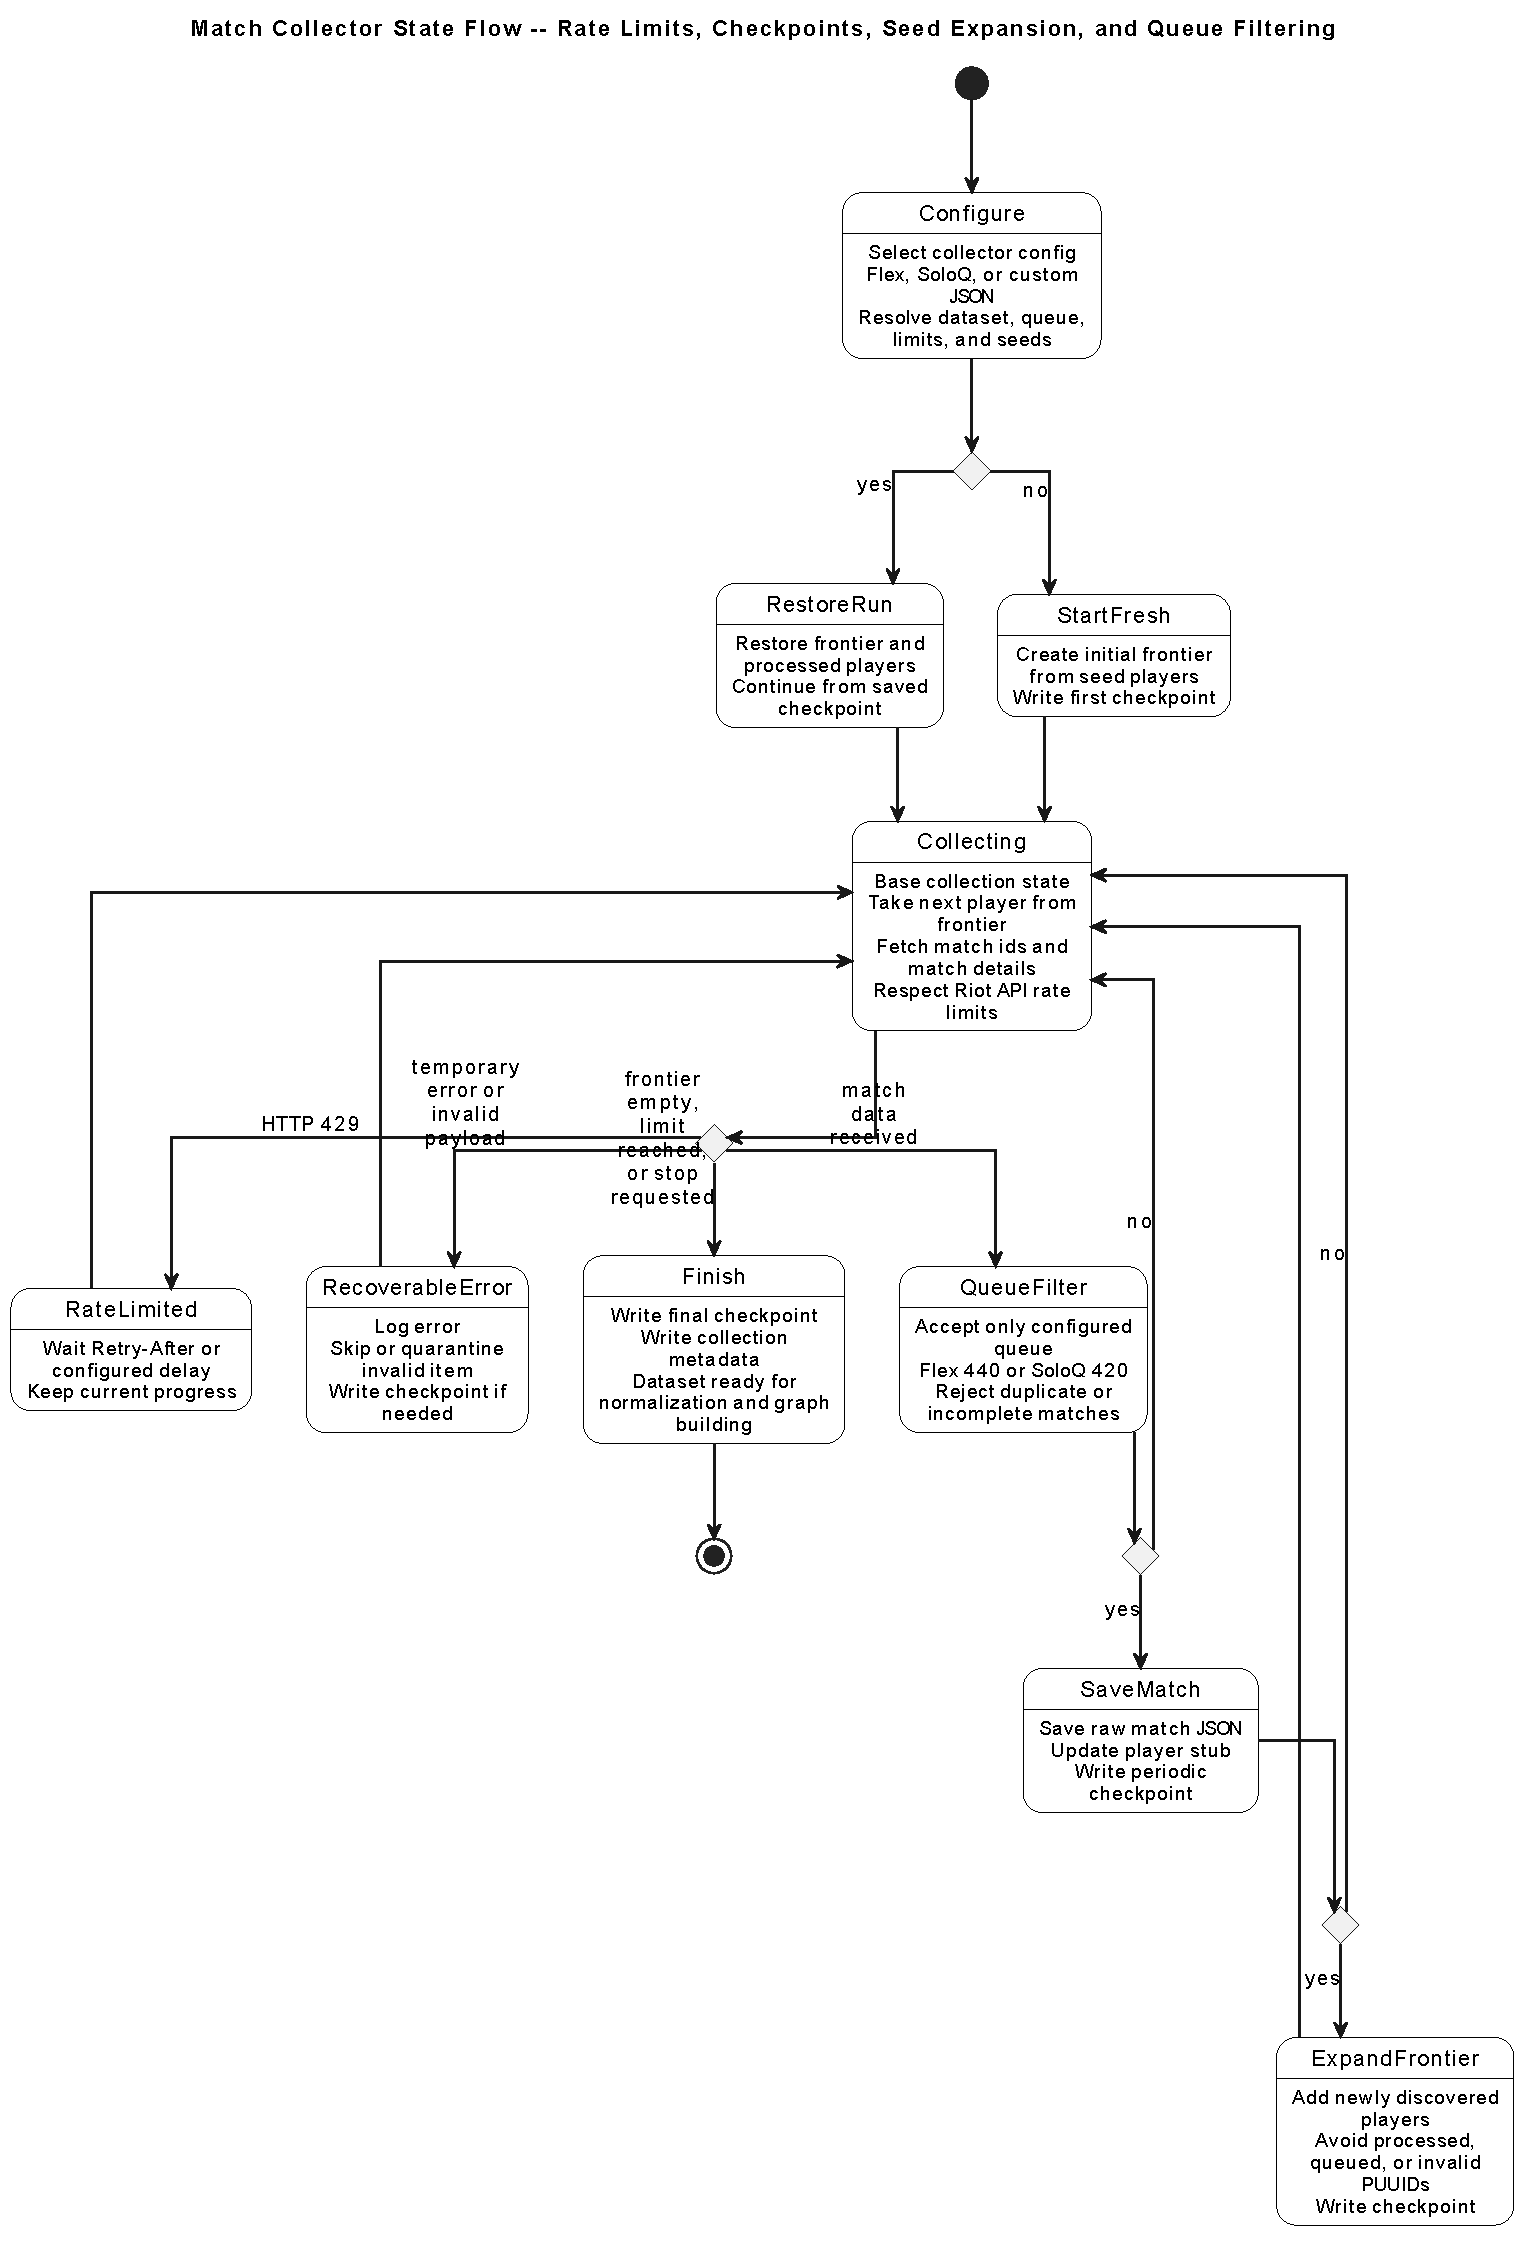
\includegraphics[width=0.98\textwidth,height=0.74\textheight,keepaspectratio]{collector-state-machine.pdf}
\caption{A collector paraméterezhető állapotgépének folyamatábrája}
\end{figure}

\section{Gyűjtési fókusz és queue-választás}

A rendszer nem a Riot teljes játékuniverzumát próbálja egyetlen adatfolyamba összesöpörni, hanem tudatosan olyan queue-típusokból építkezik, amelyekben az ismétlődő kapcsolatok és a premade-jelleg reálisabban megjelenhet. Ez az oka annak, hogy a repository dokumentációja és gyűjtőszkriptjei külön foglalkoznak az EUNE és a Master/SoloQ jellegű mintákkal, illetve a gyors tesztadatsorokkal.

A projekt korai adatgyűjtési fázisában a \texttt{default} dataset vegyes queue-tartalmat gyűjtött. A 2026. április 24-én ellenőrzött állapotban a queue-eloszlás a következő volt (ez a \texttt{default} datasetre vonatkozik, nem az aktív \texttt{soloq}/\texttt{flexset} datasetekre):

\begin{table}[H]
\centering
\caption{Queue-eloszlás az aktív \texttt{default} dataseten}
\begin{tabular}{lrr}
\toprule
\textbf{Queue ID} & \textbf{Darabszám} & \textbf{Értelmezés} \\
\midrule
420 & 1371 & Ranked Solo/Duo \\
440 & 1351 & Ranked Flex \\
450 & 358 & ARAM \\
400 & 313 & Normal Draft \\
900 & 45 & URF / rotációs mód \\
480 & 20 & Normal Blind \\
700 & 9 & Clash \\
740 & 2 & Intro/AI jellegű mód \\
870 & 2 & Egyéb speciális queue \\
\bottomrule
\end{tabular}
\end{table}

Ez két fontos dolgot jelez. Egyrészt a korpusz zöme olyan játékmódból jön, ahol a kompetitív ismétlődés reális. Másrészt a dataset vegyes: a rangsorolt játékon kívül ARAM és normál draft elemek is bekerültek. Emiatt a dolgozatban különösen fontos, hogy a gráfot ne „barátsági gráfként”, hanem ismétlődő játékkapcsolati hálóként kezeljem.

\begin{table}[H]
\centering
\caption{Térképeloszlás az aktív \texttt{default} dataseten}
\begin{tabular}{lrr}
\toprule
\textbf{Map ID} & \textbf{Darabszám} & \textbf{Értelmezés} \\
\midrule
11 & 3113 & Summoner's Rift \\
12 & 358 & Howling Abyss \\
\bottomrule
\end{tabular}
\end{table}

A map-eloszlás azt is mutatja, hogy a korpusz döntően a klasszikus Summoner's Rift környezetre épül. Ez azért lényeges, mert a szerepkörök, az útvonalkeresési interpretáció és a teljesítménymutatók is ebben a közegben a legjobban értelmezhetők.

\section{Premade-fókusz és gyűjtési stratégiai intuíció}

A projekt mögött végig ott állt az a gyakorlati intuíció, hogy az igazán érdekes kapcsolatok nem az egyszeri, véletlenszerű találkozásokból születnek, hanem a visszatérő együtt- vagy egymás ellen játszásból. Emiatt a gyűjtőszkriptek és a dokumentáció egy része kifejezetten premade-szerű vagy ismétlődő kapcsolatok felderítésére van hangolva.

Ez a szemlélet a teljes későbbi rendszerre hatással volt:

\begin{itemize}
    \item a gráfépítésben élküszöb jelent meg;
    \item az asszortativitás és a központisági elemzés az ismétlődő kapcsolatokat tekinti komoly jelöltnek;
    \item a pathfinder-költségek is a kapcsolaterősséget veszik figyelembe.
\end{itemize}

Másképp fogalmazva: a gyűjtési stratégia nem előszoba, hanem a későbbi gráfjelentés egyik meghatározó forrása.

Ez a döntés ugyanakkor tudatos torzítást is bevezet. Ha a gyűjtés a visszatérő, premade-szerű kapcsolatokat részesíti előnyben, akkor a korpusz kevésbé reprezentálja az egyszeri és lazább találkozásokat. A jelen dolgozat céljai mellett ez elfogadható kompromisszum, mert a kutatási kérdés középpontjában éppen a tartósabb kapcsolati magok állnak. A háló tehát nem a teljes populáció semleges lenyomata, hanem az ismétlődő interakciók felé célzottan dúsított részvilág.

\section{Rate limit, megbízhatóság és operatív kompromisszumok}

A Riot API használata az architektúrában nem pusztán külső függőség, hanem korlátozó tényező is. A fejlesztői kulcsok lekérdezésszámhoz kötöttek, ezért a gyűjtőrétegben explicit sebességkorlát-kezelés, várakozási logika és részfeladatokra bontás jelent meg. A dokumentációban rögzített rate-limit elemzés ezt nem adminisztratív részletként, hanem rendszertervezési kényszerként kezeli.

Ennek közvetlen következményei:

\begin{itemize}
    \item a meccsletöltés nem kérésenkénti frontend-akcióként, hanem háttérfolyamatként fut;
    \item a nyers adatállapotot érdemes lokálisan cache-elni;
    \item a grafikus és analitikai oldal nem függhet attól, hogy egy élő API-lekérés éppen sikeres-e.
\end{itemize}

Ez a döntés később az egész rendszer egyik alapelve lett: \emph{a demo- és kutatási réteg a már összegyűjtött korpuszra épül, nem online API-kérésekre}.

Az implementáció szintjén ez több konkrét védelmet jelent. A collector saját másodpercenkénti várakozást alkalmaz, külön kétperces ablakban számlálja a kéréseket, \texttt{HTTP 429} esetén harminc másodpercet vár, majd újrapróbálkozik, és a már elmentett meccseket fájllétezés alapján kihagyja. Ez a működés idempotenssé teszi a letöltést: egy megszakadt vagy újraindított futás nem írja felül feleslegesen a korábbi állományokat, és nem épít újabb bizonytalanságot a nyers korpuszba.

\begin{table}[H]
\centering
\caption{A collector fő megbízhatósági mechanizmusai}
\begin{tabularx}{\textwidth}{>{\raggedright\arraybackslash}p{4.4cm}X}
\toprule
\textbf{Mechanizmus} & \textbf{Funkció} \\
\midrule
Saját \texttt{requestsPerSecond} késleltetés & A rövid távú API-terhelés kontrollja \\
Kétperces számláló & Illeszkedés a Riot kulcshasználati limitjeihez \\
\texttt{429} újrapróbálás & Robusztusabb működés átmeneti limitütközéskor \\
Létező meccsfájl kihagyása & Duplikált mentés és újra-letöltés elkerülése \\
Eseményes stdout log & Backend- és frontend-oldali állapotkövetés támogatása \\
\bottomrule
\end{tabularx}
\end{table}

Ezek a döntések nem puszta üzemeltetési kényelmi funkciók. A reprodukálható számítógépes kutatás egyik alapelve, hogy az eredményekhez vezető lépések nyomon követhetők és lehetőleg automatizálhatók legyenek \cite{sandve2013}. A collector parametrizálhatósága, eseményes logolása és idempotens mentési logikája pontosan ezt a célt szolgálja.

\section{A flexset és a soloq gyűjtési stratégiájának összehasonlítása}

A két kutatási dataset nem véletlenszerűen jött létre, hanem eltérő gyűjtési stratégiák eredménye. Ez a különbség az analitikai eredmények értelmezéséhez is nélkülözhetetlen.

\subsection{Flexset: premade-fókuszú, apex-tier Flex Queue}

A \texttt{flexset} dataset gyűjtési konfigurációja a következő főbb stratégiai döntéseken alapul:

\begin{itemize}
    \item \textbf{Queue-szűrés}: kizárólag 440-es queue ID-jű (Ranked Flex) meccsek;
    \item \textbf{Seed-populáció}: EUNE Master+ ranglista-pozíciójú játékosok;
    \item \textbf{Premade-probe}: a collector egy rövid meccslista-minta alapján ellenőrzi, hogy a jelölt játékos rendelkezik-e elegendő ismétlődő csapattársi mintázattal. Ha igen, a teljes meccsgyűjtés megkezdődik;
    \item \textbf{Minimális premade ismétlések}: a \texttt{minimumPremadeRepeats} paraméter azokat a seedelési jelölteket vonja be, amelyeknél az ismétlődő kapcsolatok valószínűsége meghaladja a küszöböt;
    \item \textbf{Seed-terjeszkedés}: az egyes játékosok feldolgozásakor a rendszer a csapattársaik azonosítóit is felveszi a gyűjtési sorba.
\end{itemize}

Ez a stratégia egyfajta \emph{premade-központú snowball sampling}: a már gyűjtött játékosok szomszédain keresztül bővül a mintakör. Az eredmény egy erősen összefüggő, visszatérő kapcsolatokban gazdag szociális háló.

\subsection{Soloq: teljesítmény-alapvonal, kontroll-adatkészlet}

A \texttt{soloq} dataset gyűjtési konfigurációja szándékosan más fókusszal rendelkezik:

\begin{itemize}
    \item \textbf{Queue-szűrés}: kizárólag 420-as queue ID-jű (Ranked Solo/Duo) meccsek;
    \item \textbf{Seed-populáció}: EUNE Master$+$ Solo/Duo Queue ranglistán szereplő játékosok - ez \emph{nem azonos} a flexset seed-populációjával, amely a Flex Queue ranglistájára épül; a két ranglista eltérő mechanikán alapul, és eltérő játékosbázist hoz létre;
    \item \textbf{Premade-probe}: itt a probe-logika \emph{nem} szűr premade-jelenlét alapján, hanem elsősorban teljesítményadat-elérhetőség alapján;
    \item \textbf{Kisebb korpusz}: a konfigurált korlátok 2000 meccs körül zárnak le (vs. flexset 4980).
\end{itemize}

A soloq gyűjtés tehát \emph{nem premade-ra optimalizált}: a Solo/Duo Queue nem ösztönzi az 5-fős premade csapatokat, és a kollekciós stratégia sem keresi aktívan a visszatérő szövetségesi mintákat. Ez teszi a soloq-ot alkalmas kontrollalappá.

\begin{table}[H]
\centering
\caption{A két dataset gyűjtési stratégiájának összehasonlítása}
\begin{tabularx}{\textwidth}{>{\raggedright\arraybackslash}p{4.2cm} X X}
\toprule
\textbf{Dimenzió} & \textbf{flexset} & \textbf{soloq} \\
\midrule
Queue ID & 440 (Flex) & 420 (Solo/Duo) \\
Premade-probe & Igen, ismétlések alapján & Nem \\
Seed-terjeszkedés & Csapattársak alapján & Listalekéréssel \\
Gyűjtési cél & Szociális struktúra & Teljesítmény-alapvonal \\
Corpus mérete & 4980 meccs & 2000 meccs \\
Szerep a projektben & Fő kutatási adatkészlet & Kontroll-adatkészlet \\
\bottomrule
\end{tabularx}
\end{table}

Ez a kettős stratégia az egyik legfontosabb módszertani döntése a projektnek. Azzal, hogy a projekt explicit módon gyűjtötte és felcímkézte a két eltérő karakterű datasetet, lehetővé tette azt a kontrolláltabb összehasonlítást, amelynek eredményei a jelen dolgozat empirikus fejezeteit adják.

\subsection{Megállási feltételek és reprodukálhatóság}

Mindkét dataset gyűjtése a következő megállási feltételek valamelyikén áll le: elérte a konfigurált maximális meccsszámot; elérte a konfigurált maximális iterációszámot; a gyűjtési sor kiürült; vagy manuálisan le lett állítva.

A nyers meccs-JSON fájlok fájlrendszeren perzisztálódnak. Az idempotens létező-fájl-ellenőrzés garantálja, hogy már letöltött meccsek nem kerülnek újra letöltésre, ami lehetővé teszi a fokozatos, megszakítható gyűjtést.

\section{Adatminőség, torzítás és óvatos interpretáció}

A Riot API formálisan pontos, de a dolgozat szempontjából az adat így sem „semleges”. A mintavételt erősen befolyásolja:

\begin{itemize}
    \item milyen seed játékosokról indult a gyűjtés;
    \item mely queue-k kerültek előtérbe;
    \item milyen mélyre ment a meccslista-lekérés;
    \item a premade-kapcsolatok milyen minimumismétlés után tekinthetők érdekesnek.
\end{itemize}

Ezért a dolgozat minden későbbi eredményénél fontos megjegyzés, hogy a hálózat \emph{nem a teljes League of Legends univerzum reprezentációja}, hanem egy adott gyűjtési stratégia által létrehozott, vizsgálható részvilág. Ez nem gyengeség, hanem korrekt keretfeltétel.

További torzításforrás, hogy a dataset fokozatosan épülő archívumként működik. A meccsek nem egyetlen, szigorúan lezárt időablakból származnak, ezért a játékosok \texttt{match\_count} értékei részben azt is tükrözik, mennyire került rájuk fókusz a gyűjtési folyamatban. Emiatt a score-réteg és az időbeliség kapcsolatát mindig óvatosan kell kezelni: a magasabb mintaszám nem kizárólag aktivitást, hanem gyűjtési figyelmet is jelenthet.

% ===== chapters/05-a-rendszer-korai-valtozata-es-az-eredeti-pipeline.tex =====
\chapter{A rendszer korai változata és az eredeti pipeline}

\section{A korai projekt jellege}

A repository története alapján a rendszer első változata jóval közelebb állt egy adatvezérelt játékosnézőhöz és kísérleti gráf-exportáló eszközhöz, mint a jelenlegi, több rétegre bontott kutatási platformhoz. Ebben a szakaszban a cél elsősorban az volt, hogy:

\begin{itemize}
    \item a Riot API-ból érkező nyers mérkőzésadatok egy helyre kerüljenek;
    \item a játékosokhoz legalább alapvető pontszámok rendelődjenek;
    \item a kapcsolatokból egyszerű gráf és klaszterkimenet szülessen;
    \item a projekt vizuálisan is megmutatható legyen.
\end{itemize}

Ez a korai szakasz nem eldobandó előtörténet, hanem a jelenlegi rendszer kiindulópontja. A dolgozatban azért tartom meg hangsúlyosan, mert ebből érthető meg, miért alakult ki később a többnyelvű architektúra és a szigorúbb perzisztenciamodell.

\section{Az első pontozási logika}

Az eredeti \texttt{add\_new\_players.js} egyszerűbb, kézzel összeállított képletekkel dolgozott. A korai \texttt{feedscore} lényegében a halálokat büntette a kill és assist mennyiségéhez képest, míg az első \texttt{opscore} főként a következő komponensekre támaszkodott:

\begin{itemize}
    \item ölések,
    \item asszisztok,
    \item arany,
    \item vision score.
\end{itemize}

Ez a kezdeti modell nyers volt, de fontos előnye volt: gyorsan megmutatta, hogy a tiszta KDA-logikán túl is lehet értelmes, legalább részben kompozit teljesítménymutatót számolni. Később ebből nőtt ki az artifact-szintű és szerepkörérzékeny rendszer.

\section{A korai gráfépítés és export}

A korai \texttt{build\_graph.py} és a hozzá kapcsolódó exportlépések alapvetően Python-központúak voltak. A hangsúly ekkor még a gyors láthatóságon és nem a perzisztens újrafelhasználhatóságon volt. A pipeline:

\begin{itemize}
    \item meccsekből kapcsolati gráfot épített,
    \item összefüggő komponenseket és részgráfokat vizsgált,
    \item HTML és PyVis exportokat készített,
    \item gyors vizuális ellenőrzést tett lehetővé.
\end{itemize}

Ez a megközelítés jó prototípus volt, de rövid időn belül látszott a korlátja: a klaszterek és gráfnézetek csak exportként éltek tovább, és nem váltak a rendszer belső, lekérdezhető objektumaivá.

\section{A korábbi régiós és ország-alapú ág kialakulása}

A projekt korai időszakában erősebb szerepet kapott az a gondolat is, hogy a klaszterekből ország- vagy régiószintű következtetések szülessenek. Ennek nyomai ma is megtalálhatók a \texttt{fetch\_clusters.py}, \texttt{assign\_countries.py} és \texttt{conclude.py} szkriptekben. A megközelítés lényege az volt, hogy a klaszterek tagneveiből valamilyen földrajzi címke becsülhető, majd ehhez aggregált teljesítményadatok rendelhetők.

Ez a gondolat önmagában izgalmas, de a dolgozat mostani állapotában már világos, hogy módszertanilag bizonytalanabb, mint a közvetlenül a gráfstruktúrára és a meccsadatokra támaszkodó elemzések. Emiatt ezt a vonalat nem törlöm ki a történetből, hanem kifejezetten korábbi, exploratív modulként kezelem.

\section{Miért kellett a rendszert továbbépíteni?}

A korai változat legfontosabb korlátai a következők voltak:

\begin{itemize}
    \item egyetlen adatbázis és egyetlen meccskönyvtár köré szerveződött;
    \item a klaszterek és exportok nem voltak igazán első osztályú perzisztens objektumok;
    \item a pontozás még nem volt kellően szerepkörérzékeny;
    \item a futásidejű útvonalkeresés és a nehezebb gráfanalitika nem vált el élesen a frontend-logikától.
\end{itemize}

Ezek a hiányok nem kudarcot jeleztek, hanem természetes érési pontokat. A jelenlegi rendszer legjobban akkor érthető, ha nem egyetlen pillanatfelvételként, hanem ilyen fokozatos evolúció eredményeként nézzük.

Visszatekintve a projekt korai szakaszának legtermészetesebb csapdája az \emph{akkumulatív script-architectúra} lett volna, amelyben minden új feature egy újabb script formájában kerül be, és az egész rendszer globális állapottól függ. Ez a minta sok hasonló méretű adat-kutatási projektben megfigyelhető. Azzal, hogy a projekt tudatosan bevezette a dataset-absztrakciót, a Rust-szintű analitikai elválasztást és a perzisztens klasztermodellt, elkerülte ezt a csapdát.

Különösen fontos fordulópontot jelentett az a felismerés, hogy \emph{a kutatási analitikának nem szabad a frontend-állapottól függenie}. Ha az asszortativitás kiszámítása frontend-kérésre, a böngészőben lévő adatokból történne, akkor egyrészt nem lenne reprodukálható, másrészt nagyon érzékeny lenne a felhasználói interakcióra. A Rust-oldali, parancssori futtathatóság ezt a problémát gyökeresen oldja meg.

\section{Miért kellett a régi szövegréteget is megtartani?}

Szakdolgozatírás közben könnyű lenne azt a hibát elkövetni, hogy a projekt korábbi állapotát egyszerűen ``lecserélem'' a jelenlegi, erősebb verzióra. Ezt tudatosan nem teszem. A korai pipeline, a \texttt{conclude.py}-szerű ág és a régi klaszterértelmezések azért maradnak a dolgozatban, mert ezek adják meg a fejlődés irányát. A mostani rendszer nem légüres térben született, hanem ezekből nőtt ki.

A country-alapú ágat (a \texttt{assign\_countries.py} és a \texttt{conclude.py} modulokat) jelenleg elavultnak tekintem: az ország-hozzárendelés megbízhatósága nem elegendő ahhoz, hogy a projekt fő állításait erre épüljenek, és a kód aktív karbantartás nélkül is a repositoryban marad mint történeti dokumentum. Ugyanakkor az a gondolat, hogy a klasztereket értelmezési egységként kezeljük - és ne csak vizuális exportként -, ebből az ágból nőtt ki. Ebben az értelemben az ott szerzett tapasztalat a jelenlegi klasztermodel egyik alapköve.

\diagramfigure{A korai Python-alapú adatgyűjtő és gráfépítő pipeline adatáramlása}{old python graph dataflow diagram.pdf}

% ===== chapters/06-a-rendszerarchitektura-evolucioja.tex =====
\chapter{A rendszerarchitektúra evolúciója}

\section{Áttekintés}

A projekt jelenlegi architektúrája tudatosan hibrid. Első ránézésre ez bonyolultabbnak tűnhet, mint egyetlen nyelvre vagy egyetlen futtatókörnyezetre építeni mindent, de a jelen esetben éppen ez a szétválasztás teszi védhetővé a rendszert.

A feladat ugyanis több, egymástól eltérő természetű részre oszlik:

\begin{itemize}
    \item adatgyűjtés és tömeges JSON-feldolgozás;
    \item statisztikai és szerepkör-érzékeny pontszámítás;
    \item gráfépítés és klaszterezés;
    \item futási időben használható, gyors útvonalkeresés és analitika;
    \item böngészőben is jól prezentálható vizualizáció.
\end{itemize}

Ezeket a projekt az alábbi rétegek között osztja szét:

\begin{itemize}
    \item \textbf{Python}: gyűjtés, gráfépítés, közösségdetektálás, exportfolyamatok;
    \item \textbf{SQLite}: központi perzisztens tárolás;
    \item \textbf{Node.js / Express}: API-héj és orchesztráció;
    \item \textbf{Rust}: útvonalkeresés, asszortativitás, központiság, globális gráf-artifaktumok;
    \item \textbf{React + Vite}: interaktív frontend és vizuális prezentáció.
\end{itemize}

Az alábbi komponensdiagram a teljes rendszer magas szintű szerkezetét mutatja be: a Python adatgyűjtő és gráfépítő worker-eket, a Node.js/Express API réteget, a Rust analitikai motort, a React/Vite frontendet és a C\# ASP.NET Core adatbázis-böngészőt, valamint az ezeket összekötő kommunikációs csatornákat és tárolási egységeket. A diagram jól mutatja, hogy a frontend--Rust Pathfinder összeköttetés a Node.js API-n keresztül fut: a frontend közvetlenül nem hívja a Rust motort, hanem HTTP-végpontokon keresztül kommunikál a Node rétegrel, amely a Rust folyamatot stdin/stdout csatornán keresztül vezérli.

\clearpage
\begingroup
\special{papersize=210mm,430mm}
\special{pdf:put @thispage << /MediaBox [0 0 595.276 1218.898] >>}
\thispagestyle{empty}
\enlargethispage{150mm}
\begin{figure}[H]
\centering
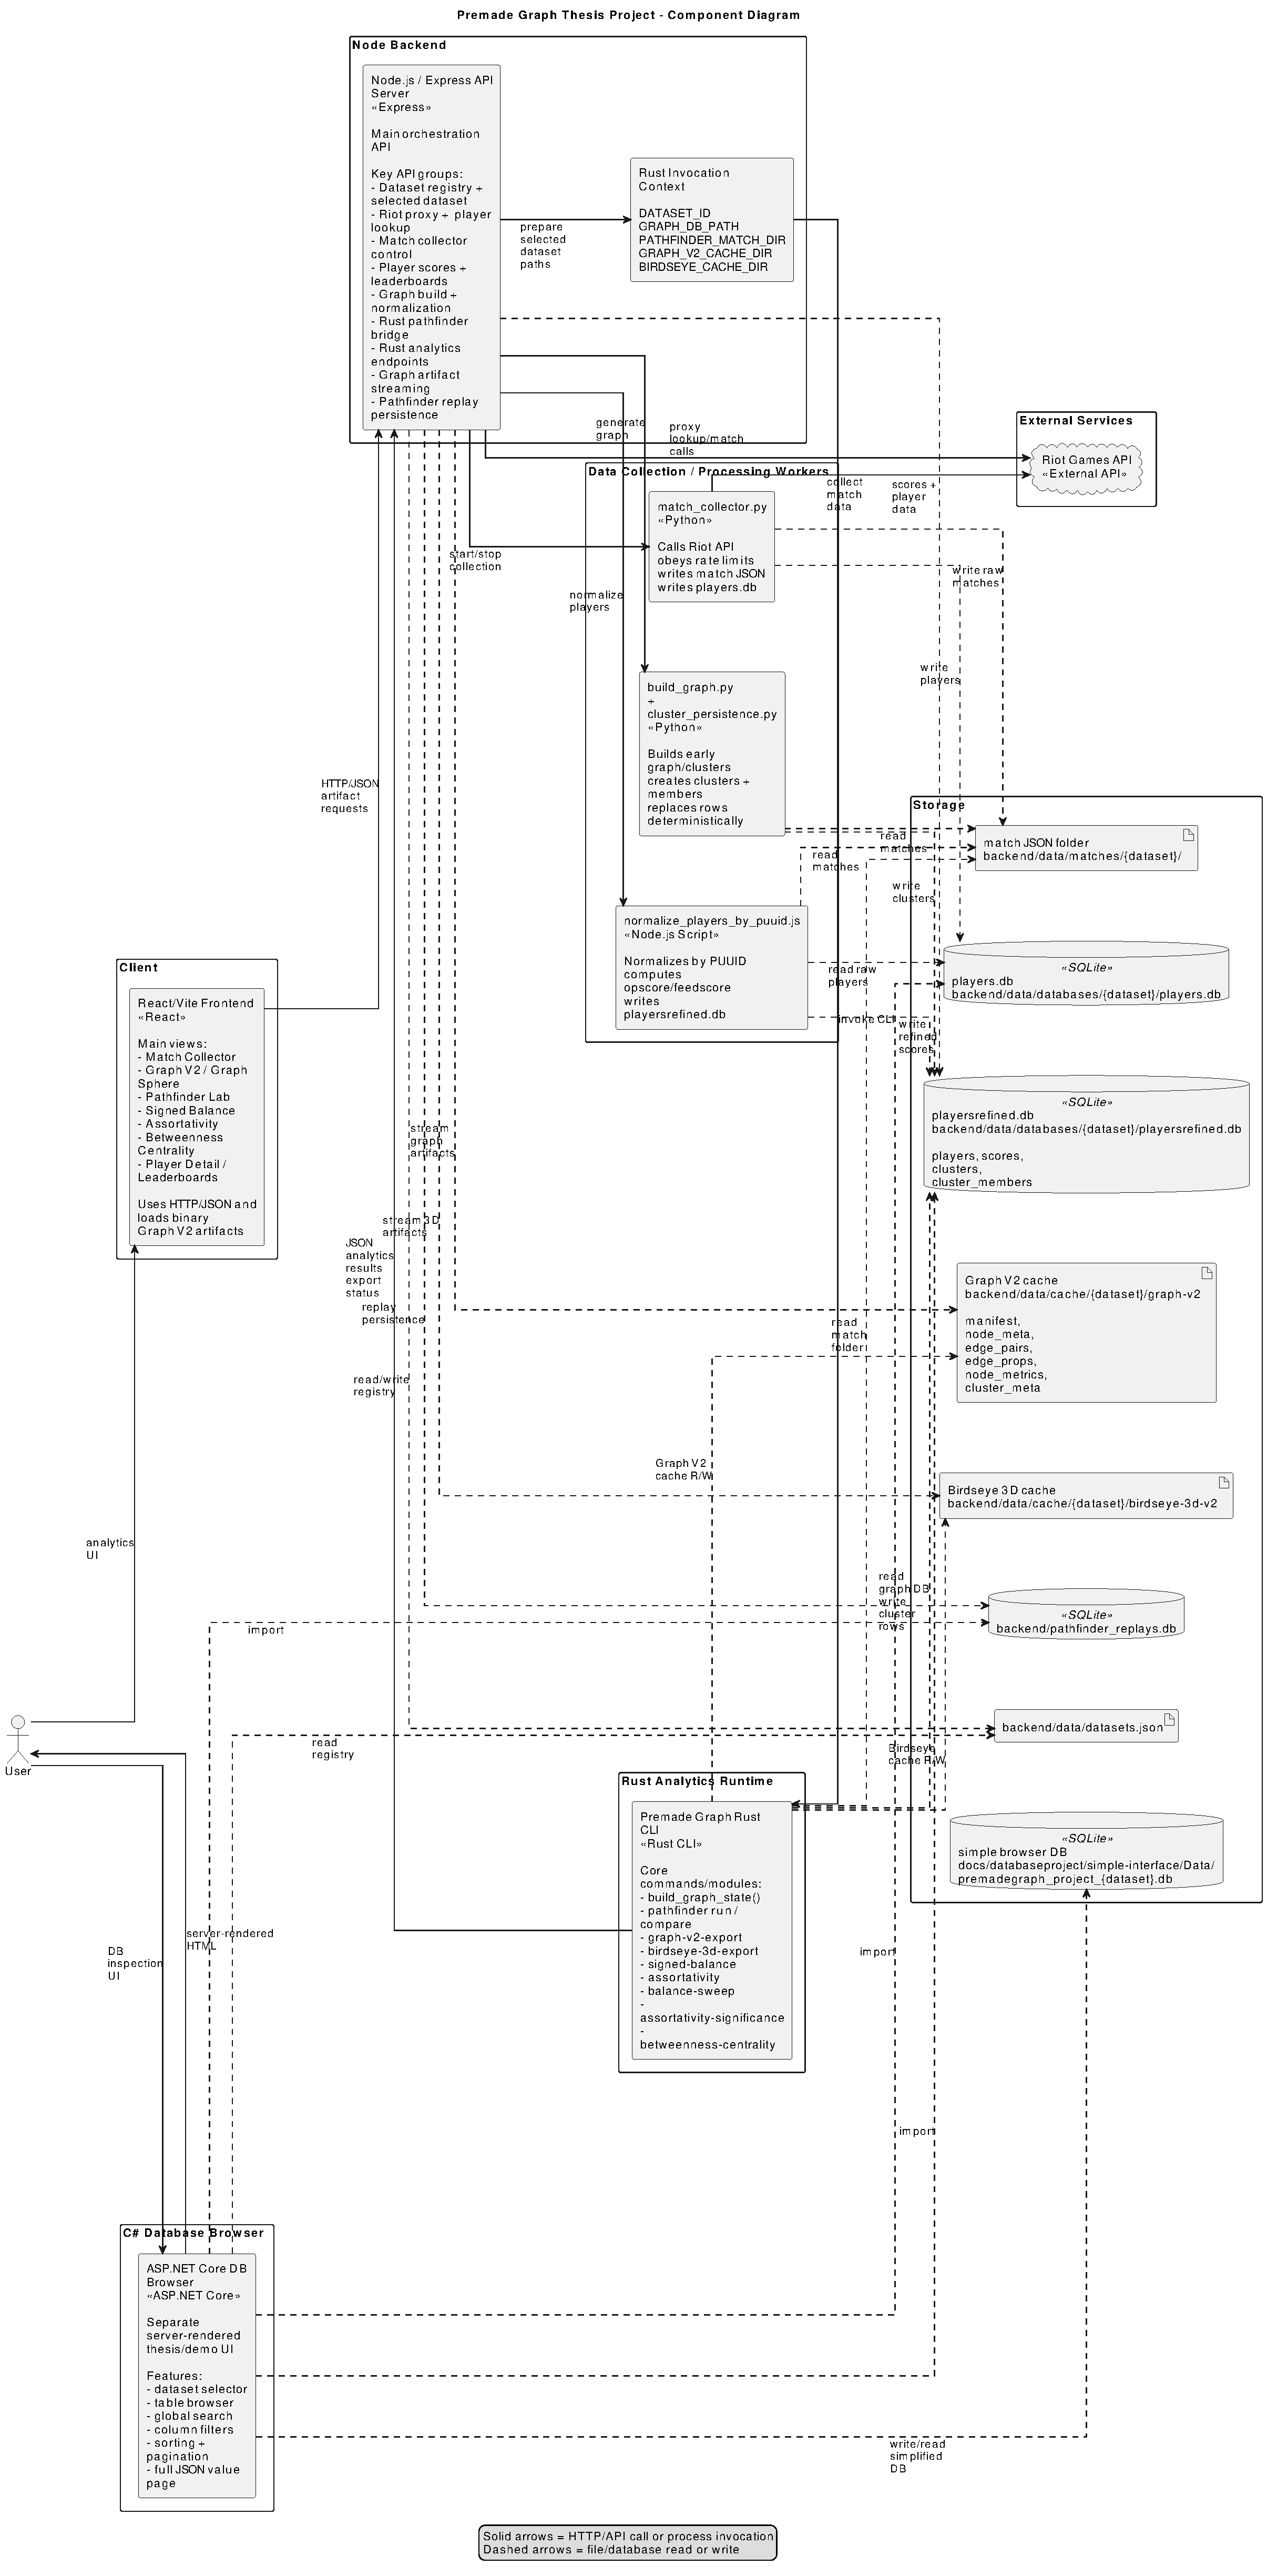
\includegraphics[width=0.98\textwidth,height=355mm,keepaspectratio]{full system diagram.pdf}
\caption{A teljes rendszer komponensdiagramja - Python worker-ek, Node.js API, Rust analitikai motor, React frontend és C\# adatbázis-böngésző}
\end{figure}
\clearpage
\endgroup
\special{papersize=210mm,297mm}

\section{Miért nem egyetlen technológia?}

A rendszer felépítésében a legfontosabb architekturális elv az volt, hogy \emph{a kontextus dönti el a technológiát}, nem fordítva. A Python kiváló az adatgyűjtéshez, a JSON-feldolgozáshoz és a hálózatépítés gyors iterációjához. A Rust viszont sokkal alkalmasabb a nagyméretű, ismételten meghívott gráfalgoritmusokhoz, ahol fontos a determinisztikus viselkedés, a teljesítmény és a strukturált export. Az SQLite kis projektméret mellett is kényelmesen biztosítja a perzisztenciát, a React pedig jó eszköz a demo- és elemzőfelületek építéséhez.

Ez a szétválasztás nem „tech stack gyűjtögetés”, hanem tudatos munkamegosztás:

\begin{itemize}
    \item az adatfeldolgozó lépések külön újrafuttathatók,
    \item a számításigényes részek nincsenek a böngészőre tolva,
    \item az eredményeket tárolni, exportálni és később újrafelhasználni is lehet.
\end{itemize}

\subsection{Miért maradt a C\# böngésző különálló, és nem integrálódott a fő frontend-be?}

A C\# / ASP.NET Core adatbázis-böngésző tudatosan különálló eszközként él. A fő frontend (React / Vite) kutatási és vizualizációs célú: gráfnézetek, pathfinder, asszortativitás és betweenness-központiság. A böngésző ezzel szemben \emph{adatbázis-inspekciós} eszköz: nyers táblasorok, JSON-értékek, szűrés, lapozás. Ezek különböző felhasználói igényeket elégítenek ki, és különböző technológiai stack-et igényelnek. Egy React-ba beágyazott adatbázis-nézet könnyen bonyolítaná a frontend bundle-t, miközben az ASP.NET Core-os szerver-oldali megközelítés JavaScriptes kliensoldali logika nélkül is stabil, könnyen telepíthető eszközt ad.

\subsection{Elvetett architekturális alternatívák}

A végső döntés mellett az elutasított alternatívákat is érdemes dokumentálni. A projekt fejlődése során legalább négy természetes irány merülhetett volna fel:

\begin{table}[H]
\centering
\caption{Fontos architekturális alternatívák és elutasításuk oka}
\begin{tabularx}{\textwidth}{>{\raggedright\arraybackslash}p{3.5cm} >{\raggedright\arraybackslash}p{3.6cm} X}
\toprule
\textbf{Alternatíva} & \textbf{Rövid előny} & \textbf{Miért nem ez lett a végső irány?} \\
\midrule
Minden Pythonban & Gyorsabb kezdeti iteráció & A futásidejű gráfalgoritmusoknál és a nagyobb exportoknál gyengébb teljesítmény- és memóriakontroll \\
Minden Rustban & Erős típusosság és egységes motor & A gyűjtés és a gyors kísérletezés jelentősen nehezebbé és lassabbá vált volna \\
Frontend-központú számítás & Egyszerűbb demoarchitektúra & A böngészőre tolta volna a számításigényes gráfmunkát, gyengítve a reprodukálhatóságot \\
Szerveres SQL-adatbázis & Erősebb többfelhasználós modell & A projekt lokális, bemutatható és kutatásorientált természete mellett az SQLite kedvezőbb kompromisszum maradt \\
\bottomrule
\end{tabularx}
\end{table}

Különösen fontos itt a Python és Rust közti munkamegosztás. A Python megőrizte a gyors adatmanipuláció és prototípuskészítés előnyeit, míg a Rust a stabil futásidejű gráfmag szerepét kapta. A kettő közé a Node/Express réteg került, amely szerződéses API-határként működik.

\subsection{Miért maradt a Node középen?}

Felmerülhetne, hogy a frontend miért nem közvetlenül a Rust motorral kommunikál, vagy miért nem a Python szolgálja ki a teljes alkalmazást. A \texttt{backend/server.js} alapján a Node rétegnek önálló felelőssége van:

\begin{itemize}
    \item dataset-regisztert kezel és aktív datasetet választ;
    \item futás közbeni kulcsokat és környezeti útvonalakat központosít;
    \item háttércollector folyamatokat indít és monitoroz;
    \item HTTP-végpontokat biztosít a Rust parancsok fölé;
    \item a bird's-eye artifaktumokat és egyéb cache-eket konzisztensen szolgálja ki.
\end{itemize}

Ez a köztes réteg csökkenti a frontend és a számítási mag közti csatolást. A böngészőnek nem kell folyamatindítással, fájlrendszer-útvonalakkal vagy dataset-propagálással foglalkoznia; ezek a backendben maradnak.

\section{Evolúciós fázisok és architekturális kompromisszumok}

Az architektúra fejlődését három, viszonylag jól elkülöníthető fázisban lehet leírni.

\begin{enumerate}
    \item \textbf{Korai script-fázis}: a hangsúly a nyers adat begyűjtésén, a gyors score-számításon és a kezdeti gráfexporton volt.
    \item \textbf{Perzisztens pipeline-fázis}: megjelent az igény arra, hogy a klaszterek és játékosprofilok ne csak pillanatnyi exportként, hanem visszatölthető adatstruktúraként éljenek tovább.
    \item \textbf{Kutatási platform-fázis}: a Rust analitika, a multi-dataset modell és a külön research oldalak megjelenésével a projekt már nem csak vizualizációs eszköz, hanem kísérleti környezet lett.
\end{enumerate}

Minden fázisban más minőségi attribútum került előtérbe: először a fejlesztési sebesség, utána a reprodukálhatóság, végül a teljesítmény és az elemzési mélység. Ez segít megérteni, miért nem ``inkonzisztencia'' a több réteg, hanem a rendszer természetes evolúciója.

\section{Több-adatkészletes architektúra}

A korábbi, egyetlen adatbázisra és egyetlen meccsmappára épülő modell helyett a jelenlegi rendszer már több, egymástól független adatkészletet támogat. A \texttt{backend/data/datasets.json} regiszter alapján minden dataset külön rendelkezik:

\begin{itemize}
    \item nyers adatbázissal,
    \item finomított adatbázissal,
    \item meccs-JSON könyvtárral,
    \item cache könyvtárral.
\end{itemize}

A dolgozat írásakor az aktív dataset a \texttt{default} azonosítójú alap-adatkészlet volt, de a regiszterben a \texttt{smoke-test-dataset} és a \texttt{flexset} is szerepel. Ez fontos előrelépés a korábbi állapothoz képest, mert lehetővé teszi, hogy különböző mintákon, különböző gyűjtési stratégiákkal is fusson ugyanaz az analitikai pipeline.

\begin{table}[H]
\centering
\caption{A több-adatkészletes architektúra logikai elemei}
\begin{tabularx}{\textwidth}{>{\raggedright\arraybackslash}p{3.2cm}X}
\toprule
\textbf{Elem} & \textbf{Szerep} \\
\midrule
Dataset registry & Az elérhető adatkészletek metaadatait és az aktív dataset kijelölését tárolja \\
Raw database & A gyűjtéshez és kezdeti beolvasáshoz szükséges játékosadatok \\
Refined database & A normalizált pontszámokat, klasztereket és származtatott mezőket tartalmazza \\
Matches directory & A tényleges meccs-JSON állományok helye \\
Cache directory & Futás közbeni vagy előre generált artifaktumok tárolása \\
\bottomrule
\end{tabularx}
\end{table}

\subsection{A dataset mint életciklus-egység}

A dataset a jelenlegi rendszerben nem statikus mappát, hanem együtt mozgó állapotcsomagot jelent. Egy új dataset létrehozása után több, egymástól elválasztható fázison mehet keresztül:

\begin{enumerate}
    \item nyers seed és játékosállapot kialakítása;
    \item match collector futtatása;
    \item PUUID-alapú normalizálás és score-frissítés;
    \item legacy Python export vagy populációs klaszterperzisztencia, ha az adott futás ezt igényli;
    \item Rust runtime-felépítés, Graph V2 artifact-export és bird's-eye export;
    \item kutatási analitikák lefuttatása.
\end{enumerate}

Ez a bontás a dolgozat szempontjából azért erős, mert világos köztes állapotokat ad. Egy asszortativitási vagy központisági futtatásnak nem kell újra elindítania a Riot API-gyűjtést, és egy klaszterezési változtatásnak sem kell a teljes pipeline-t újraépítenie. A dataset tehát a reprodukálható munkafolyamat egységeként is értelmezhető.

\begin{figure}[H]
\centering
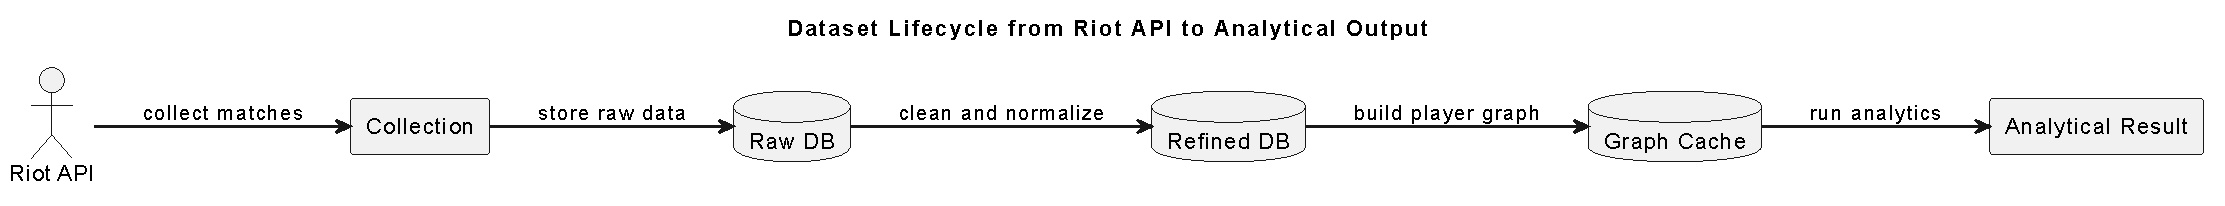
\includegraphics[width=0.98\textwidth,height=0.74\textheight,keepaspectratio]{dataset lifecycle riotapi to analytical output.pdf}
\caption{Egy dataset teljes életciklusának diagramja a Riot API-tól az analitikai kimenetig}
\end{figure}

\section{A jelenlegi adatállapot}

Az aktív adatállapotot 2026. április 28-án közvetlenül a repository aktuális állapotából ellenőriztem. Az aktív dataset a \texttt{soloq}. Az ellenőrzött fő adatállományok és adatbázisok adatai:

\textbf{Flexset dataset (EUNE Master+ Flex Queue):}
\begin{itemize}
    \item meccs-JSON állományok: \textbf{4981} fájl a \texttt{backend/data/matches/flexset/} könyvtárban;
    \item Graph V2 összegző jelentés: \texttt{matchCount: 4980} (egy fájl eltérés ellenőrizendő);
    \item nyers adatbázis (\texttt{players.db}): \textbf{15\,147} játékos;
    \item finomított adatbázis (\texttt{playersrefined.db}): \textbf{15\,421} játékos, \textbf{599} klaszter, \textbf{5741} klasztertag.
\end{itemize}

\textbf{SoloQ dataset (EUNE Master+ Solo/Duo Queue, aktív):}
\begin{itemize}
    \item meccs-JSON állományok: \textbf{2001} fájl a \texttt{backend/data/matches/soloq/} könyvtárban;
    \item Graph V2 összegző jelentés: \texttt{matchCount: 2000};
    \item nyers adatbázis (\texttt{players.db}): \textbf{2822} játékos;
    \item finomított adatbázis (\texttt{playersrefined.db}): \textbf{6768} játékos, \textbf{140} klaszter, \textbf{1538} klasztertag.
\end{itemize}

Fontos megjegyezni, hogy a soloq dataset klaszterei jellemzően \emph{duo párokat} jelölnek: mivel a Solo/Duo Queue maximálisan kétfős premade csapatokat enged, az ismétlődő kapcsolatokból kiemelkedő klaszterek döntő többsége két-három játékosra szűkül. Ez strukturálisan különbözik a flexset klasztereitől, ahol akár ötfős premade csapat is kialakulhat rendszeresen ismétlődő együttsként.

Ez a pont fontos: a jelen dolgozat nem hipotetikus rendszert ír le, hanem egy olyan állapotot, amelyben a pipeline már nem csak tervekből áll, hanem két, egymással összehasonlítható, eltérő queue-szemantikájú, valós adatokkal feltöltött és ténylegesen lefuttatott kutatási korpusszal rendelkezik.

A meccsszámban megfigyelhető egy-fájlos eltérés (4981 fájl vs. 4980 matchCount a Graph V2 összegzőben) metodikai megjegyzést igényel: ez feltehetően egy olyan meccsfájl, amelyet a gyűjtő letöltött, de a Graph V2 pipeline valamilyen validációs szűrőn kizárt. Ez nem kritikus eltérés, de jól mutatja, hogy a pipeline nem pusztán fájlszámlálás alapján dolgozik.

\section{Perzisztencia és relációs modell}

A projekt egyik legfontosabb érése az volt, hogy a klaszterek kikerültek a „csak JSON export” kategóriából, és első osztályú adatbázis-objektumokká váltak. A jelenlegi séma központi táblái az SQLite perzisztenciára épülnek \cite{sqlite}:

\begin{itemize}
    \item \texttt{players},
    \item \texttt{clusters},
    \item \texttt{cluster\_members}.
\end{itemize}

A \texttt{players} tábla nemcsak a név- és országmezőket, hanem a normalizált \texttt{opscore}, \texttt{feedscore}, szerepkör, meccsszám és artifact-szintű részeredményeket is tárolja. A \texttt{clusters} és \texttt{cluster\_members} páros pedig lehetővé teszi, hogy ugyanazon játékoshoz többféle klasztertípus (\texttt{python\_population}, \texttt{rust\_pathfinding}) is kötődjön.

\begin{figure}[H]
\centering
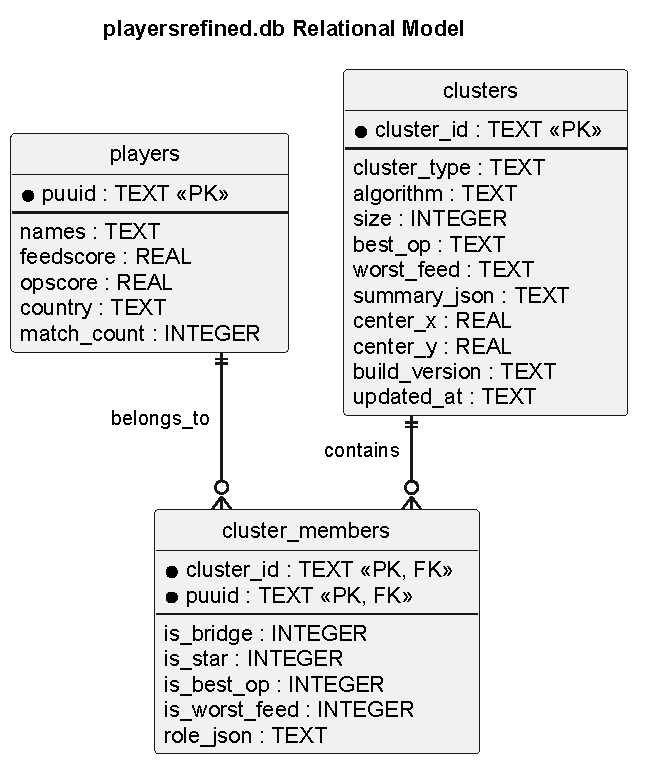
\includegraphics[width=0.68\textwidth]{relational model diagram.pdf}
\caption{Relációs modell a klaszter- és játékosperzisztenciához (\texttt{players}, \texttt{clusters}, \texttt{cluster\_members})}
\end{figure}

% ===== chapters/07-tobb-adatkeszletes-architektura.tex =====
\chapter{Több-adatkészletes architektúra}

\section{Miért vált szükségessé a dataset-regiszter?}

Az egyetlen adatbázisos modell korai prototípushoz még elegendő volt, de amint a projekt egyszerre kezdett demo-, smoke-test- és kutatási célokat szolgálni, világossá vált, hogy a különböző minták szétválasztása nélkül a rendszer nehezen reprodukálható. Ugyanaz a frontend, ugyanaz a Rust futtatókörnyezet és ugyanaz a Python pipeline más eredményt adhat, ha eltérő bemeneti korpuszon fut. Ezt a különbséget nem rejtett konfigurációs fájlokban, hanem explicit dataset-regiszterben érdemes kezelni.

A dataset-regiszter bevezetésének szükségességét konkrét igényváltozás indokolta:

\begin{itemize}
    \item \textbf{Smoke-teszt igény}: a fejlesztői pipeline-t kis adathalmazzal kell tudni validálni, anélkül hogy az éles adatbázist módosítani kellene;
    \item \textbf{Kutatási szétválasztás}: a Flex Queue és a Solo/Duo Queue strukturálisan eltérő gráfot hoz létre; az eredmények összekeveredése módszertanilag hibás lenne;
    \item \textbf{Reprodukálhatósági garancia}: ha a fő kutatási dataset változik, a régi dataset-állapot is ellenőrizhető maradjon;
    \item \textbf{Pipeline-átjárhatóság}: a Rust analitika, a Python klaszterpipeline és a Node/Express API mind ugyanarra a dataset-re álljon rá, ne legyen ``backend igazság'' és ``Rust igazság'' egymás mellett.
\end{itemize}

Az \textbf{elvetett alternatíva} a konfigurációs fájlon alapuló manuális váltás lett volna: a felhasználó kézzel módosít egy útvonalat, és a rendszer azt használja. Ez nem skálázódik, mert a több állapot egyszerre való megtartása nem lehetséges, és az összekeveredési hibák nehezen detektálhatók.

A \texttt{backend/data/datasets.json} pontosan ezt a feladatot látja el. A dataset fogalma a jelenlegi rendszerben nem csak annyit jelent, hogy ``másik mappa'', hanem egy teljes, együtt mozgó adategységet:

\begin{itemize}
    \item nyers adatbázissal,
    \item finomított adatbázissal,
    \item meccs-JSON könyvtárral,
    \item cache-könyvtárral,
    \item megjeleníthető metaadatokkal.
\end{itemize}

\section{A jelenlegi regiszterben szereplő adatkészletek}

A dolgozat írásakor ellenőrzött \texttt{backend/data/datasets.json} regiszterben négy dataset szerepelt:

\begin{itemize}
    \item \texttt{default} - az eredeti telepítésből migrált, vegyes queue-tartalmú alapkorpusz;
    \item \texttt{smoke-test-dataset} - gyors infrastruktúratesztelésre szánt átmeneti adatkészlet;
    \item \texttt{flexset} - EUNE Master$+$ Flex Queue meccsek, kifejezetten premade és ismétlődő csapattársi kapcsolatok tanulmányozására;
    \item \texttt{soloq} - EUNE Master$+$ Solo/Duo Queue meccsek, kontroll- és teljesítmény-alapvonal-gyűjtés céljából.
\end{itemize}

Az \textbf{aktív dataset a \texttt{soloq}}. Ez a döntés az adatbázis-regiszterben is rögzített: a \texttt{currentDatasetId} mező értéke \texttt{"soloq"}.

A négy dataset jelenléte nem véletlen felhalmozódás, hanem tudatos kutatásstratégia eredménye. A \texttt{default} megőrzi az eredeti, heterogén korpuszt és a korábbi fejlesztési előtörténetet. A \texttt{smoke-test-dataset} a pipeline gyors ellenőrzésére szolgál anélkül, hogy a főadatokat érintené. A \texttt{flexset} és a \texttt{soloq} egymással párban értelmezhetők: az előbbi a premade és csoportos játékhoz kötődő társas jeleket erősíti, az utóbbi pedig ugyanannak a szervernek és rangsornak egyénibb, kevésbé premade-fókuszú meccstörténetét képviseli.

\begin{table}[H]
\centering
\caption{A négy regisztrált dataset összefoglalója}
\begin{tabularx}{\textwidth}{>{\raggedright\arraybackslash}p{3.0cm} >{\raggedright\arraybackslash}p{3.0cm} X}
\toprule
\textbf{Dataset ID} & \textbf{Szerepkör} & \textbf{Jellemzők} \\
\midrule
\texttt{default} & Alap/migrált & Vegyes queue, heterogén tartalom \\
\texttt{smoke-test} & Pipeline-teszt & Átmeneti, infrastruktúra-validálásra \\
\texttt{flexset} & Fő kutatási dataset & EUNE Master$+$ Flex, premade-fókusz \\
\texttt{soloq} & Kontroll/baseline & EUNE Master$+$ Solo/Duo, teljesítmény-alap \\
\bottomrule
\end{tabularx}
\end{table}

A \texttt{flexset} esetében a regiszter metaadata tartalmazza a gyűjtési stratégia dokumentumát és a collector konfigurációs fájl hivatkozását (\texttt{apex\allowbreak-flex\allowbreak-collector.json}). A \texttt{soloq} hasonlóan strukturált: külön collector konfigurációs fájllal és gyűjtési stratégia-dokumentummal rendelkezik. Ez a párhuzamos konfiguráció kifejezetten mutatja, hogy a két dataset nem eseti gyűjtés, hanem tudatosan eltérő stratégiával felépített, összehasonlítható korpusz.

\begin{table}[H]
\centering
\caption{A dataset-regiszter funkcionális szerepei}
\begin{tabularx}{\textwidth}{>{\raggedright\arraybackslash}p{4.2cm}X}
\toprule
\textbf{Funkció} & \textbf{Jelentőség} \\
\midrule
Aktív dataset kijelölése & Meghatározza, hogy a backend és a frontend mely adatkorpuszt használja alapértelmezetten \\
Eltérő tárolási útvonalak & Megakadályozza, hogy a teszt- és főadatok összekeveredjenek \\
Külön cache-ek & A bird's-eye és egyéb előre generált artifaktumok elkülönülnek \\
Kísérleti összevethetőség & Azonos pipeline különböző mintákon is futtatható \\
\bottomrule
\end{tabularx}
\end{table}

\section{A dataset-választás propagálása a backend és a Rust felé}

A dataset-ek architektúrájának egyik legfontosabb technikai előnye az, hogy a választás nem áll meg a Node-szinten. A backend a kiválasztott datasetből környezeti változókat és útvonalakat képez a Rust futtatókörnyezet felé is, például:

\begin{itemize}
    \item \texttt{DATASET\_ID},
    \item \texttt{GRAPH\_DB\_PATH},
    \item \texttt{PATHFINDER\_MATCH\_DIR},
    \item \texttt{PATHFINDER\_BIRDSEYE\_CACHE\_DIR}.
\end{itemize}

Ez építészetileg nagyon fontos döntés. Nincs külön ``frontend igazság'', ``backend igazság'' és ``Rust igazság'' ugyanarról az adatállapotról: a dataset-választás a teljes végrehajtási láncon végigmegy.

A \texttt{server.js} szintjén ez úgy valósul meg, hogy a szerver a kiválasztott datasetből egységes környezeti változókészletet képez, például \texttt{DATASET\_ID}, \texttt{GRAPH\_DB\_PATH}, \texttt{PATHFINDER\_MATCH\_DIR} és \texttt{PATHFINDER\_BIRDSEYE\_CACHE\_DIR} formában. A Rust runtime ezeket fogyasztja, így a teljes végrehajtási lánc ugyanarra az adatvilágra áll rá. Ez különösen fontos a védhetőség szempontjából: a frontend által mutatott eredmény nem különálló demonstrációs adatból, hanem ugyanabból a datasetből jön, amelyen a kutatási analitika is fut.

% ===== chapters/08-sqlite-perzisztencia-es-klasztermodellezes.tex =====
\chapter{SQLite perzisztencia és klasztermodellezés}

\section{Miért maradt központi elem az SQLite?}

A projekt mérete és célja szempontjából az SQLite továbbra is kifejezetten jó kompromisszum. Nem igényel külön adatbázisszerver-felügyeletet, könnyen verziózható a séma, gyors a lokális fejlesztésben, és a demo közben sincs szükség külön infrastruktúrára. Ennél is fontosabb, hogy a perzisztens modell egyszerűen ellenőrizhető: a játékos-, klaszter- és tagsági sorok közvetlenül lekérdezhetők.

Egy szakdolgozatban ez külön előny. Nem csak a frontend JSON-kimeneteit lehet megmutatni, hanem az alapul szolgáló relációs tárolást is.

\begin{figure}[H]
\centering
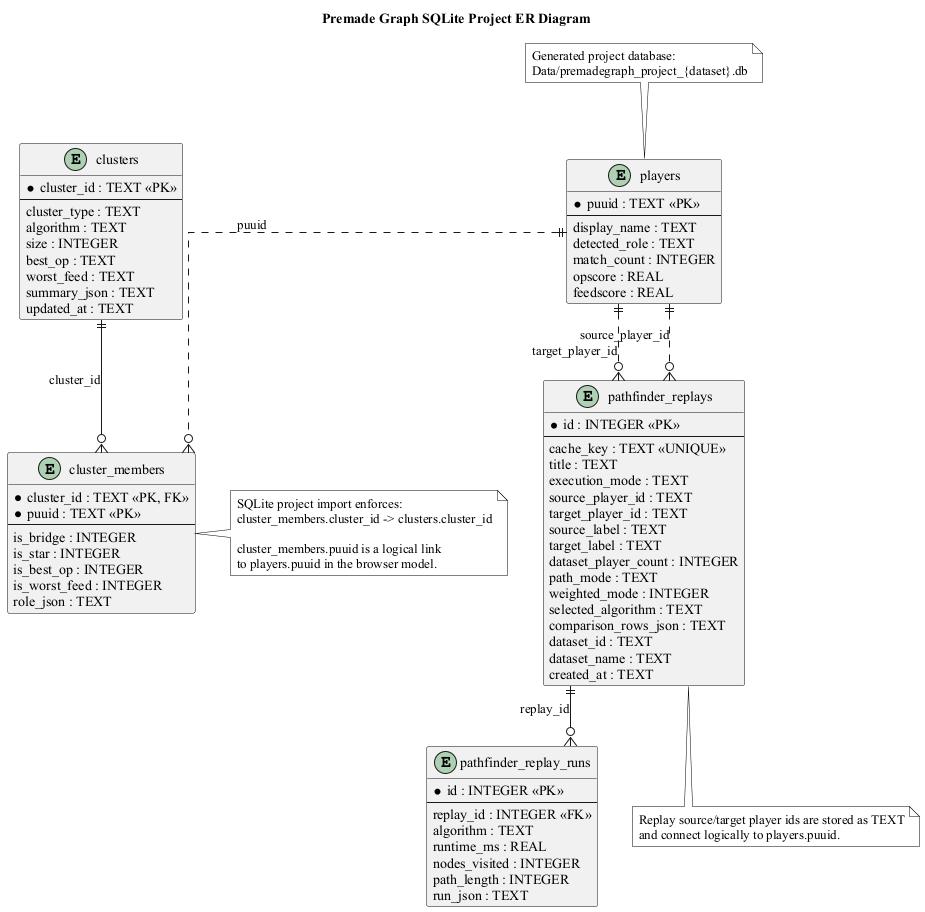
\includegraphics[width=0.98\textwidth,height=0.76\textheight,keepaspectratio]{sqlite-project-er-diagram.png}
\caption{A fő SQLite adatbázis egyedkapcsolati diagramja}
\end{figure}

\section{A \texttt{players} tábla mint gazdagított játékosprofil}

A jelenlegi \texttt{players} tábla már jóval több egy egyszerű névjegyzéknél. A fő mezőcsoportok:

\begin{itemize}
    \item azonosítók és névmezők;
    \item aggregált teljesítménymutatók (\texttt{feedscore}, \texttt{opscore});
    \item mintanagyságot leíró mezők (\texttt{match\_count}, \texttt{matches\_processed});
    \item szerepkör és szerepkör-bizonyosság;
    \item artifact-szintű komponensek.
\end{itemize}

A 2026. április 24-én vizsgált állapotban a tábla \textbf{25\,618} játékost tartalmazott. A szerepkör-eloszlás közel kiegyensúlyozott képet mutatott a fő lane-szerepkörök között, miközben \texttt{UNKNOWN} kategóriába is került \textbf{3120} játékos. Ez a gyakorlatban azt jelenti, hogy a rendszer nem próbál mindenáron erőltetett lane-hozzárendelést végezni ott, ahol a nyers adat nem kellően megbízható.

\begin{table}[H]
\centering
\caption{Szerepkör-eloszlás a vizsgált \texttt{players} állapotban}
\begin{tabular}{lr}
\toprule
\textbf{Szerepkör} & \textbf{Játékosok száma} \\
\midrule
TOP & 4571 \\
MIDDLE & 4517 \\
JUNGLE & 4484 \\
BOTTOM & 4471 \\
UTILITY & 4455 \\
UNKNOWN & 3120 \\
\bottomrule
\end{tabular}
\end{table}

\subsection{Sémanormalizáció és visszafelé kompatibilitás}

A \texttt{backend/normalize\_players\_by\_puuid.js} egyik fontos, de könnyen rejtve maradó tulajdonsága, hogy nem tiszta, egyszer létrehozott sémával számol. A modul deklarálja a \texttt{players} tábla kanonikus oszlopkészletét, és szükség esetén a történetileg felhalmozott eltérésekhez is alkalmazkodik. Ez a projekt evolúciós természetéből következik: a score-réteg, a szerepkörmezők és az artifact-szintű komponensek nem egyszerre, hanem fokozatosan kerültek be a modellbe.

Ennek szakdolgozati jelentősége is van. A rendszer nem laboratóriumi körülmények között egyszer megtervezett és lezárt adatbázissal dolgozik, hanem olyan struktúrával, amely a fejlesztés közben bővült. A normalizáló modul ezért egyben migrációs réteg is: megőrzi a régebbi állapotok használhatóságát, miközben előkészíti az újabb analitikai mezőket.

\subsection{SQLite pragmák és írási kompromisszumok}

A normalizáló pipeline az SQLite-ot nem alapbeállításokkal használja. A kód explicit módon \texttt{WAL} naplózást, \texttt{NORMAL} szinkronizációt, memóriabeli ideiglenes tárolást és foreign key támogatást állít be. Ez a választás jól mutatja, hogy az SQLite jelenléte nem „egyszerűségi lustaság”, hanem tudatos kompromisszum. A rendszernek lokálisan futó, ismételten újraíró, de nem többszáz egyidejű felhasználót kiszolgáló analitikai adattárra van szüksége; erre a célra ez a konfiguráció kifejezetten jó arányt ad a sebesség, a stabilitás és a hordozhatóság között.

\section{A klasztermodell és a két fő tábla szerepe}

A klaszterek perzisztenciáját a \texttt{clusters} és \texttt{cluster\_members} páros adja. A \texttt{clusters} tábla főbb elemei:

\begin{itemize}
    \item \texttt{cluster\_id},
    \item \texttt{cluster\_type},
    \item \texttt{algorithm},
    \item \texttt{size},
    \item \texttt{summary\_json},
    \item térbeli koordináták,
    \item build-verzió és frissítési idő.
\end{itemize}

A \texttt{cluster\_members} tábla ezzel szemben tagsági és szerepkörjellegű információt tárol:

\begin{itemize}
    \item a klaszter és játékos összerendelését;
    \item \texttt{is\_bridge}, \texttt{is\_star}, \texttt{is\_best\_op}, \texttt{is\_worst\_feed} jelzőket;
    \item szerepköri összegzést \texttt{role\_json} formában.
\end{itemize}

Ez a modell azért erős, mert a klaszter nem puszta név vagy címke, hanem lekérdezhető objektum, amelyhez külön metaadatok és tagsági szerepek kötődnek.

A \texttt{backend/cluster\_persistence.py} további fontos döntése, hogy a klaszterek cseréjét \texttt{cluster\_type} szerint végzi. Vagyis egy új \texttt{python\_population} build felülírja a régi Python-klasztereket, de nem nyúl a \texttt{rust\_pathfinding} családhoz. A művelet előbb törli az adott típushoz tartozó régi tagsági sorokat, majd a klasztermetaadatokat, és ezután írja be az új eredményt. Ez a szemantika nagyon hasznos, mert ugyanazon adatbázisban több klasztercsalád élhet együtt anélkül, hogy egy újrafuttatás mindent elsöpörne.

A \texttt{summary\_json}, \texttt{role\_json}, \texttt{build\_version} és \texttt{updated\_at} mezők a kutatási visszakövethetőséget is javítják. A klaszter így nem pusztán tagsági halmaz, hanem olyan objektum, amelynek eredete, típusa és részleges összefoglaló állapota is megmarad.

\section{A perzisztált klaszterek aktuális nagyságrendje}

A két fő kutatási dataset finomított adatbázisainak ellenőrzött állapota alapján a klaszterstruktúra lényegesen eltér a két korpuszban:

\textbf{Flexset} (\texttt{playersrefined.db}):
\begin{itemize}
    \item \textbf{599} klaszter a \texttt{clusters} táblában;
    \item \textbf{5741} klasztertagsági rekord a \texttt{cluster\_members} táblában;
    \item a Graph V2 artfaktumban \textbf{1531} látható klaszter, átlagos méret \textbf{3.750}, legnagyobb \textbf{20}.
\end{itemize}

\textbf{SoloQ} (\texttt{playersrefined.db}):
\begin{itemize}
    \item \textbf{140} klaszter a \texttt{clusters} táblában;
    \item \textbf{1538} klasztertagsági rekord a \texttt{cluster\_members} táblában;
    \item a Graph V2 artfaktumban \textbf{870} látható klaszter, átlagos méret \textbf{1.768}, legnagyobb \textbf{20}.
\end{itemize}

A két szám közötti különbség metodikailag fontos. A \texttt{clusters} táblában tárolt klaszterek a Python pipeline által meghatározott, populációs alapú közösségek. A Graph V2 látható klasztereinek száma magasabb, mert a Graph V2 külön, kötetlen ally-csoportként kezeli azokat a csomópontokat is, amelyek csak vizualizációs szempontból alkotnak csoportot. A flexset lényegesen sűrűbb klaszterstruktúrát mutat: az átlagos klaszterméret (3.750) a soloq-hoz képest (1.768) közel duplája, ami empirikusan is alátámasztja, hogy a Flex Queue erősebb ismétlődő csoportkapcsolatokat termel.

Ez önmagában is fontos rendszerszintű eredmény, mert mutatja, hogy a többdataset-architektúra valódi különbséget fog meg, nem csupán méretbeli eltérést.

\section{A két klasztercsalád részletes összehasonlítása}

A rendszerben két klasztercsalád él párhuzamosan, amelyek különböző módszerrel és célra épülnek:

\subsection{python\_population}

A \texttt{python\_population} típusú klaszterek a korai Python gráfépítési pipeline kimenetei. Ezeket a \texttt{backend/build\_graph.py} jellegű modulok és NetworkX-alapú modularitási közösségdetektálás hozzák létre a nyers meccsadatok alapján. Főbb jellemzők:

\begin{itemize}
    \item a klaszterméret nincs kemény korláthoz kötve (a moduláris detektálás saját maga dönt a méretekről);
    \item az algoritmus a globális moduláris optimalizáció szempontjából határozza meg a csoportokat;
    \item a flexset dataseten például közepes méretű, $\sim$10--15 fős klaszterek is keletkezhetnek, ha a moduláris struktúra azt indokolja;
    \item a Python klaszterek inkább \emph{közösségdetektálási} perspektívát tükröznek.
\end{itemize}

\subsection{rust\_pathfinding}

A \texttt{rust\_pathfinding} típusú klaszterek a Rust motor futásidejű klaszterezési logikájából jönnek. Az implementáció az ally-kapcsolatokon alapuló erős-összefüggési szegmensekre bontja a gráfot, kemény méretkorláttal (maximum 20 tag). Főbb jellemzők:

\begin{itemize}
    \item a 20 tagos korlát garantálja a klaszterek áttekinthetőségét a frontend vizualizációban;
    \item az oversized összefüggő komponensek determinisztikusan kerülnek szétvágásra;
    \item a Rust klaszterek főként \emph{pathfinding és vizualizációs} célra optimalizáltak;
    \item az \texttt{orbitScore} és \texttt{orbitRadius} értékek kizárólag a Rust klaszterekre értelmezhetők.
\end{itemize}

\subsection{A két csomád koegzisztenciájának módszertani értéke}

A két klasztercsalád nem egymást helyettesíti, hanem egymást kiegészíti. A Python klaszterek adnak egy moduláris alapú közösségstruktúrát; a Rust klaszterek ennek futásidejű, vizualizáció-kompatibilis változatát. Az a tény, hogy mindkét klaszter-nézet egyszerre létezik az adatbázisban, lehetővé teszi, hogy például az asszortativitási bontásoknál explicit módon megkérdezhetjük: a Python-közösségek belső éleire vagy a Rust-vizualizációs csoportok belső éleire mért asszortativitás-e erősebb?

\section{Miért fontos a perzisztencia a kutatási fejezetekhez?}

Az asszortativitási, központisági és kísérleti signed-balance számítások látszólag a Rust oldalon történnek, de valójában a korábban kialakított perzisztens modell nélkül sokkal nehezebben lennének értelmezhetők. A klaszterekhez kötött bontások, a játékosprofilokhoz rendelt score-ok és a későbbi exportok mind arra támaszkodnak, hogy a játékos és a közösségi kontextus ugyanabban a perzisztens rendszerben elérhető.

Ez jó példa arra, hogy az adatbázistervezés nem csak kiszolgáló infrastruktúra, hanem a kutatási érték egyik feltétele.

% ===== chapters/09-az-opscore-teljesitmenymetrika.tex =====
\chapter{Az opscore teljesítménymetrika}

\section{Gyűjtési stratégia}

A projekt adatgyűjtő rétege a Riot API-ra épül. A jelenlegi architektúrában a meccsek begyűjtése nem egyetlen frontend gombnyomásra történő monolitikus folyamat, hanem paraméterezhető háttérfeladat, amely a datasethez kötve fut. A backend oldalon a gyűjtéshez tartozik:

\begin{itemize}
    \item aktív dataset kiválasztása,
    \item lekérdezési limit figyelembevétele,
    \item iterációszám és meccsszám paraméterezése,
    \item queue-típus szerinti szűrés,
    \item véletlen vagy konkrét játékos-alapú indítás.
\end{itemize}

Ez azért fontos, mert a Riot API korlátai mellett csak olyan rendszer tartható karban hosszabb távon, amely a gyűjtést külön modulnak tekinti, és nem keveri össze a futási idejű vizualizációval.

\section{Normalizálás PUUID alapján}

A nyers adatok összefűzésének kulcsa a \texttt{puuid} alapú normalizálás. A játékosnevek változhatnak, a különböző meccsekben eltérő formában is megjelenhetnek, ezért a rendszer az egyedi azonosítót tekinti az elsődleges kulcsnak. A normalizálás során a pipeline:

\begin{itemize}
    \item végigolvassa a meccs-JSON fájlokat,
    \item résztvevőnként kinyeri a releváns mezőket,
    \item szerepkört rendel a \texttt{teamPosition} alapján,
    \item meccsszintű artifactokat számol,
    \item játékosszinten átlagol és normalizál,
    \item a végeredményt a \texttt{players} táblába írja vissza.
\end{itemize}

Ez adja a rendszer egyik központi alapját, mert minden későbbi gráfanalitika erre a normalizált játékosprofilra támaszkodik.

\section{A teljesítménymetrika szükségessége}

A gráfanalitikai elemzés alapanyagát egy értelmes, szerepkörérzékeny teljesítménypontszám jelenti. A League of Legends meccsek nyers adatai -- ölések, halálok, arany, sebzés -- önmagukban nem hordoznak elegendő szemantikát: egy support 2 halála nem ugyanolyan értelmű, mint egy ADC 2 halála, egy jungler alacsony CS-értéke nem büntetendő ugyanúgy, mint egy laneré, és egy split-pusher alacsony csapaterősítő statisztikái nem feltétlenül jelzik gyenge meccsteljesítményt. Ahhoz, hogy a játékosokat egy gráfban összehasonlítható csúcsokként lehessen kezelni, szükség van egy olyan mutatóra, amely a meccsstatisztikákat szerepkör-specifikus elvárások alapján értelmezi.

Az \texttt{opscore} célja ezért nem az, hogy abszolút igazságmértékként funkcionáljon, hanem az, hogy egy következetes, értelmezhető és módszertanilag védhető skálát hozzon létre. Ez a skála az asszortativitási elemzés, a centralitásvizsgálat és az esetleges szimulációs seeding alapjaként szolgál. A metrika akkor tekinthető hasznosnak, ha különböző játékosokhoz és különböző meccsekhez következetesen rendel értelmes értékeket -- függetlenül attól, hogy az aktuális adatbázis éppen erős vagy gyenge játékosokból áll.

\section{A korábbi modell módszertani korlátai}

A modell fejlesztése fokozatos módszertani finomítás eredménye volt. A kiindulópontot egy nyolc-artifactos rendszer adta, amely szerepkör-szorzókat alkalmazott, majd a kapott nyers összegeket az adatbázis percentilis-eloszlásához viszonyítva normalizálta a $[0,10]$ tartományra. Ebben a korábbi modellben az eredmény három horgonyhoz igazodott: az 5.~percentilishez, a mediánhoz és a 95.~percentilishez; a medián játékos körülbelül $6{,}6$-os értékre esett.

Bár ez a megközelítés működőképes volt, két alapvető gyengeség hamar felszínre került.

\paragraph{Adatbázis-relatív normalizálás.}
Ha az adatbázis túlnyomórészt nagyon erős játékosokat tartalmaz, a medián játékos is a skála közepe körüli értéket kap -- hiába teljesít objektív szempontból kiemelkedően. Fordítva: ha az adatbázis viszonylag gyengébb játékosokból áll, ugyanaz a mediánteljesítmény szintén a skála közepén jelenik meg. Egy Challenger-szintű dataseten belüli medián és egy Bronze-szintű dataseten belüli medián numerikusan közel eshet egymáshoz -- ez azonban nem teljesítményállítás, csupán adatbázis-relatív elhelyezkedés. A gráfanalitika szempontjából ez különösen problematikus, mert az asszortativitás és a centralitás értelmezéséhez stabil, adatbázisfüggetlen teljesítménycímkékre van szükség.

\paragraph{A korábbi halálokon alapuló közelítés korlátai.}
A korábbi rendszer a halálokat és a kill-participationt egy külön, szándékosan minimális formulával értékelte, amely a halálokat büntette, a kill-participationt engedményként kezelte. Ez a közelítés azonban nem tudott különbséget tenni az alábbi, szemantikailag eltérő szituációk között:
\begin{itemize}
    \item egy tank, amely csapattársi nyomást vesz magára és ezzel lehetővé teszi a csapat manőverét;
    \item egy support, aki helyes engage-beállítás közben hal meg;
    \item egy split-pusher, aki szándékosan kerüli a csatatereket, de struktúrákon keresztül nyeri a meccset;
    \item egy carry, aki a meccs eldöntése után hal meg a késői fázisban;
    \item és egy ténylegesen alacsony értékű feeder, aki ismételten tempót ajándékoz az ellenfeleknek.
\end{itemize}
A korábbi képlet ezeket az eseteket nem tudta megkülönböztetni, mert nem vette figyelembe a meccs hosszát, a halálok eltöltött idejét, a szerepköri elvárásokat, a csapaterőhöz való viszonyt, vagy azt, hogy a halálokat ellensúlyozta-e valamilyen win condition-beváltás. Ez módszertani gyengeség, amelyet a jelenlegi modell strukturálisan orvosol.

Egy harmadik korlát az volt, hogy a korábbi rendszerben az artifactok értékét egy merev felső korlát szorította: minden artifact maximális hozzájárulása közel azonos volt. Ez elfedte az elité, win-condition-szintű teljesítményeket -- például egy extrém KDA-val rendelkező carry meccset, amelyet a korábbi modell középszerű értékre komprimálhatott.

\section{A helyi, szerepkörérzékeny opscore modell}

A jelenlegi \texttt{opscore} modell ezeket a korlátokat a következő tervezési elvek mentén kezeli.

\paragraph{Lokális, adatbázis-független értékelés.}
Az értékelés alapja a szerepkör-specifikus elvárás, nem az aktuális adatbázis eloszlása. Egy meccs teljesítménye értékelhető közvetlenül a meccsen belüli kontextusból, anélkül, hogy tudni kellene, kik is vannak jelen az adatbázisban. Az adatbázis-átlagok továbbra is hasznosak diagnosztikai összehasonlításra, de nem határozzák meg a jegyet.

\paragraph{Öt artifact, tíz alkategória.}
A teljesítményt öt értelmező artifact fogja át, amelyek mindegyike két alkategóriára bontódik. Ez a szerkezet elég részletes ahhoz, hogy különböző playstyle-okat megkülönböztessen, de elég átlátható ahhoz, hogy a végeredmény értelmezhetőségét megőrizze.

\paragraph{Logaritmikus bővítés elité teljesítményeknél.}
Az artifactokhoz nominális $[0, 2]$ ponttartomány tartozik, de kivételes teljesítmény esetén ez a korlát kontrolláltan átléphető. Csak a végső \texttt{opscore} van keményen korlátozva $10$-re.

\paragraph{Rövid meccsek megbízhatósági kezelése.}
A percenkénti mutatók labilis becslők rövid meccsekben. A modell egy megbízhatósági szorzóval simítja el a rövid meccsek outlier értékeit, ezáltal megelőzve, hogy egy 15 perces korai megadás irreális szélső pontszámot eredményezzen.

Az implementáció a \texttt{backend/scoring\_config.js}, a \texttt{backend/lib/scoring\_utils.js} és a \texttt{backend/normalize\_players\_by\_puuid.js} fájlokban van rögzítve.

\section{Az öt artifact és alkategóriáik}

\begin{figure}[H]
\centering
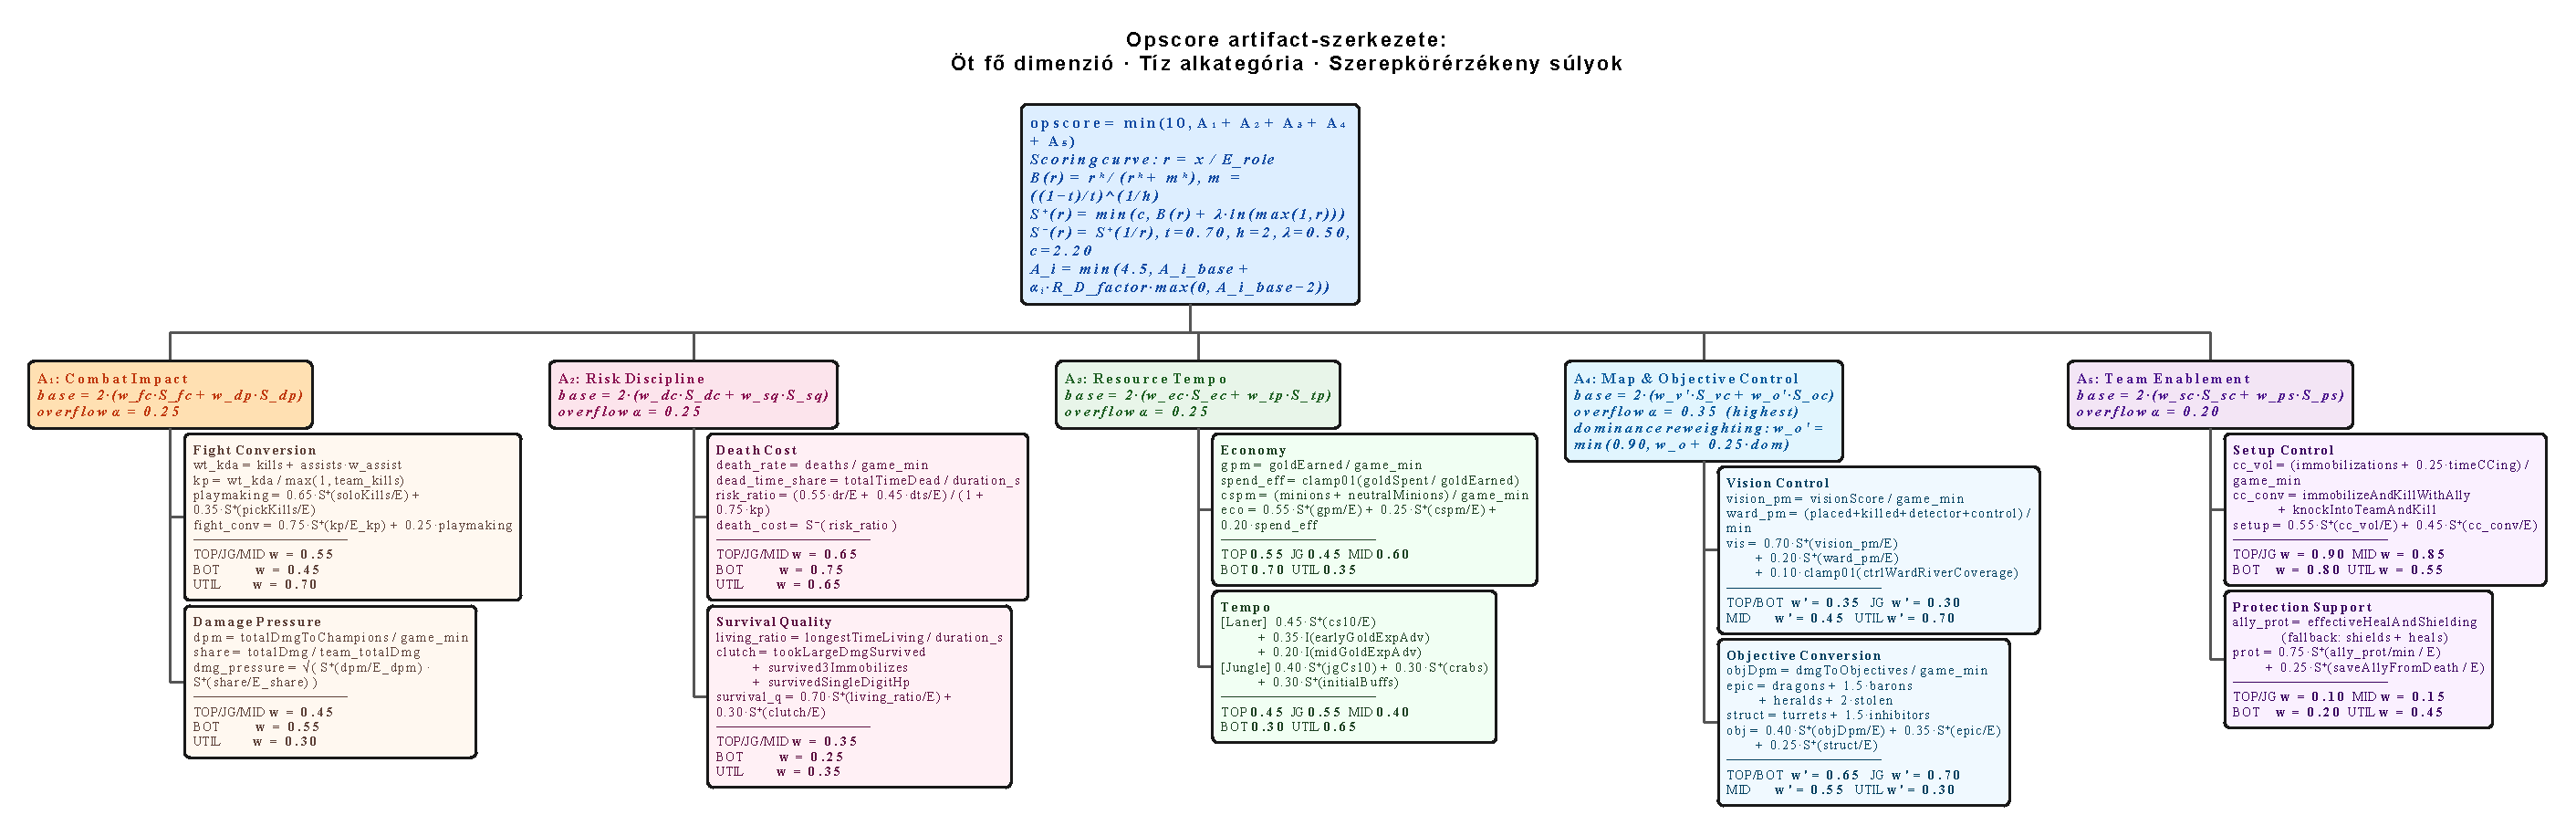
\includegraphics[width=0.98\textwidth,height=0.76\textheight,keepaspectratio]{opscore-artifacts.pdf}
\caption{Az opscore artifact-szerkezete: öt fő dimenzió, tíz alkategória, szerepkörérzékeny súlyok}
\end{figure}

A modell öt artifactból épül fel. Minden artifact két alkategóriából áll, amelyek szerepkörönként eltérő súllyal járulnak hozzá az artifact értékéhez.

\subsection{\texttt{Combat Impact}}

A \texttt{Combat Impact} artifact azt méri, hogy a játékos mennyire hatékonyan konvertálta harcait, és mekkora sebzési nyomást volt képes fenntartani.

Az első alkategória, a \emph{Fight Conversion}, a kill-participation és a csapaterőhöz viszonyított súlyozott takedown-arány alapján értékel. Emellett figyelembe veszi a solo kill és a szövetségessel együtt végrehajtott megölések arányát, mint a harckezdeményezési és döntési képesség mutatóit.

A második alkategória, a \emph{Damage Pressure}, a percenkénti sebzés és a csapaton belüli sebzési arány geometriai közepét veszi alapul. Ez azt jutalmazza, ha a játékos egyszerre hordoz magas abszolút sebzési szintet és magas csapaton belüli relatív részesedést.

A TOP, JUNGLE és MIDDLE szerepköröknél a Fight Conversion kissé nagyobb súlyt kap; az ADC esetén a Damage Pressure dominál; a support esetén a Fight Conversion kapja a nagyobb súlyt, mert a support harckonverziós hozzájárulása értékelhetőbb, mint a jellemzően alacsony abszolút sebzése.

\subsection{\texttt{Risk Discipline}}

A \texttt{Risk Discipline} artifact azt méri, hogy a játékos mennyire költségesen halt meg, és milyen túlélési minőséget produkált. Ez az artifact veszi át a korábbi halálokon alapuló mutató szerepét, de jóval kifejezőbben és részletesebben.

Az első alkategória, a \emph{Death Cost}, a percenkénti halálrátát és a meccs során holtan töltött időarányt kombinálja. Kulcsfontosságú finomítás, hogy a halálok „ára" mérséklődik, ha a játékos magas kill-participationt mutat -- azaz ha a halálokat kompenzált harckonverzió kísérte.

A második alkategória, a \emph{Survival Quality}, a meccs során életben töltött leghosszabb folyamatos időszak arányát és a kritikus szituációkban felmutatott túlélési eseményeket méri: alacsony HP-val való túlélés, több immobilizáció túlélése, csapdahelyzetből való kiszabadulás.

Az ADC esetén a Death Cost súlya a legmagasabb, mert az ADC halálai különösen drágák csapaterőhöz képest. A többi szerepkörnél a két alkategória kisebb súlyarány-különbséggel szerepel.

\subsection{\texttt{Resource Tempo}}

A \texttt{Resource Tempo} artifact a játékos gazdasági hatékonyságát és korai ritmusmegszerzési képességét értékeli.

Az \emph{Economy} alkategória a percenkénti aranytermelést, a CS-teljesítményt és az aranyköltési hatékonyságot foglalja össze. A support esetén a CS-súly minimálisra csökken, és a gold-ráfordítás hatékonysága kap nagyobb hangsúlyt.

A \emph{Tempo} alkategória lanereket és junglert eltérően értékel. Lanerek esetén a korai CS előnyt, a korai arany/tapasztalat előnyt és az ösvényfázis végén fenntartott előnyt méri. Jungler esetén az első 10 percben megszerzett dzsungelmobokat, a korai rákok és buffok megszerzését veszi alapul.

\subsection{\texttt{Map and Objective Control}}

A \texttt{Map and Objective Control} artifact azt méri, hogy a játékos mennyire járult hozzá a térképkontrollhoz és az objektívumok megszerzéséhez.

A \emph{Vision Control} alkategória a percenkénti vision score-t, a ward-aktivitás intenzitását és a kontrollward-lefedettséget kombinálja. A support esetén ennek az alkategóriának a súlya a legmagasabb.

Az \emph{Objective Conversion} alkategória az objektívumkárt, az epic-szörny részvételt (sárkányok, báró, herald, ellopott objektívumok) és a struktúrarombolást (tornyok, inhibitorok) súlyozza.

Ez az artifact tartalmaz egy dinamikus dominancia-újrasúlyozást is: ha az \emph{Objective Conversion} lényegesen meghaladja a \emph{Vision Control} alkategória értékét, az artifact automatikusan az objektívumszerzés felé tolja a súlyt. Ez azért fontos, mert a split-pusher és az objektívumcarry playstyle leírható úgy, mint ahol az Objective Conversion az elsődleges win condition -- ilyen esetben az alacsony vision aktivitás nem bünteti indokolatlanul a játékost.

A \texttt{Map and Objective Control} artifact kapja a legmagasabb overflow-erősséget, mert az objektív- és struktúranyomás közvetlen nyerési feltétel lehet.

\subsection{\texttt{Team Enablement}}

A \texttt{Team Enablement} artifact a csapattársak számára teremtett értéket méri, mind az aktív cselekvő, mind a védelmező-kiszolgáló szerepben.

A \emph{Setup Control} alkategória a percenkénti CC-aktivitást (immobilizálások, időszakos hatások) és a CC-konverziót -- azaz a CC utáni ölésbenyomás-hatékonyságot -- veszi alapul. Ez az alkategória az összes szerepkör esetén domináns; a support kapja a legkiegyensúlyozottabb arányokat a két alkategória között.

A \emph{Protection Support} alkategória a szövetségesre átadott gyógyítást és pajzsot, illetve a szövetséges haláltól való megmentésének eseményeit értékeli. A support esetén ez az alkategória kap a legnagyobb relatív súlyt.

\section{Matematikai formalizmus}

\subsection{A szerepköri arány és az alapgörbe}

Minden alkategória értékelésének kiindulópontja a megfigyelt érték és a szerepköri elvárás hányadosa:

\begin{equation}
r = \frac{x}{E_{\text{role}}}
\end{equation}

ahol $x$ a meccsen mért értéke az adott mutatónak, $E_{\text{role}}$ pedig a szerepkörhöz tartozó elvárás. Az $r = 1$ érték azt jelenti, hogy a játékos pontosan elérte a szerepköri elvárást; $r > 1$ esetén felülteljesítés, $r < 1$ esetén alulteljesítés áll fenn.

Az $E_{\text{role}}$ értékek kézileg kalibrált konstansok, amelyek a modell rögzítésének időpontjában érvényes játékmechanikára és metára támaszkodnak. A League of Legends rendszeresen kap patch-eket, amelyek megváltoztathatják az egyes szerepkörök tipikus arany-, sebzés- vagy visionértékeit. Ezért a modell akkor érvényes, ha az elvárások az aktuális játékverzióhoz kötöttek; jelentős patch után az $E_{\text{role}}$ paramétereket újra kell kalibrálni. Ez a korlát az összes szerepkör-specifikus elvárást érinti: a jelenlegi értékek a gyűjtési időszak során érvényes meta-állapothoz vannak igazítva.

Az alapgörbe egy kétparaméteres, S-alakú válaszfüggvény, amelynek középpontja a várható teljesítményszinthez igazodik:

\begin{equation}
m = \left(\frac{1-t}{t}\right)^{1/h}
\end{equation}

\begin{equation}
B(r) = \frac{r^h}{r^h + m^h}
\end{equation}

ahol $t = 0{,}70$ azt fejezi ki, hogy a várható teljesítményszint ($r = 1$) az alkategória-pontszám 70\%-át kapja, $h = 2$ pedig a görbe meredekségét szabályozza. Könnyen belátható, hogy $B(1) = 1/(1 + (1-t)/t) = t$\,: a görbe konstruálása pontosan azt biztosítja, hogy az elváráshoz igazodó teljesítmény a skála 70\%-án üljön.

Pozitív mutatóknál -- ahol a nagyobb érték jobb -- a teljes pontozási függvény:

\begin{equation}
S_+(r) = \min\!\left(c,\; B(r) + \lambda \cdot \ln\!\left(\max(1,\, r)\right)\right)
\end{equation}

ahol $\lambda = 0{,}50$ a logaritmikus bővítés erőssége és $c = 2{,}20$ az alkategória felső korlátja. A $\ln(\max(1, r))$ tag a várható szint feletti teljesítményt jutalmazza lassan növekvő, de korlátlan formában -- egészen addig, amíg a $c$ plafon be nem lép. Ez a logaritmikus rész teremti meg a modell elité carry potenciálját anélkül, hogy egyetlen nyers statisztika korlátlanul uralhatná a végeredményt.

Negatív mutatóknál -- ahol a kisebb érték jobb, például a halálráta esetén --:

\begin{equation}
S_-(r) = S_+\!\left(\frac{1}{r}\right)
\end{equation}

Ez az inverzarány-transzformáció azt biztosítja, hogy az alulteljesítők alacsony pontszámot kapjanak, az elvárás alatt maradó halálrátájú játékosok pedig magasat, a pozitív görbéhez teljesen szimmetrikusan.

\subsection{Időtartam-megbízhatóság}

Rövid meccsekben -- különösen korai megadásnál -- a percenkénti mutatók rendkívül labilis becslők. Egy 15 perces meccsben mért percenkénti arányszám jóval kevésbé stabil, mint egy 35 percesben mért ugyanaz. Ennek kezelésére a modell egy megbízhatósági szorzót vezet be:

\begin{equation}
R_D = \operatorname{clamp}_{[0,1]}\!\left(\frac{D - 12}{8}\right)
\end{equation}

ahol $D$ a meccs hossza percben. Ez a szorzó $D \le 12$ percnél nulla, $D = 15$ percnél $0{,}375$, $D \ge 20$ percnél $1{,}0$.

Az ingadozásra érzékeny percenkénti mutatók esetén az alkategória-pontszámot a megbízhatósági szorzóval súlyozza a modell egy semleges érték felé:

\begin{equation}
\tilde{S} = R_D \cdot S + (1 - R_D) \cdot 0{,}70
\end{equation}

A $0{,}70$-es semleges érték a várható teljesítményszintnek felel meg: rövid meccsekben az ingadozó mutatók automatikusan az elváráshoz közeli értékre húzódnak vissza, ezáltal megelőzve az irreálisan magas vagy alacsony percenkénti arányokból eredő torz pontszámokat. Az objektívumszerzési és struktúrarombolási eseményeket (torony, inhibitor, báró, sárkány stb.) ez a simítás nem érinti, mivel ezek diszkrét, önmagukban értékelhető események.

\subsection{Artifact-aggregáció és bővítés}

Minden artifact két alkategória súlyozott összegéből indul ki:

\begin{equation}
A_i^{\text{alap}} = 2\,(w_1 \cdot S_1 + w_2 \cdot S_2)
\end{equation}

ahol $w_1 + w_2 = 1$ és a $2$-es szorzó a nominális artifactértéket a $[0, 2]$ tartományra skálázza. Az $S_1, S_2$ értékek az adott alkategória pontozási görbéjéből adódnak, időtartam-megbízhatósági simítással, ahol szükséges.

Az elité teljesítmény kezelésére minden artifact logaritmikus bővítést kap. Ehhez egy rövidmeccs-csillapítási szorzó is szükséges:

\begin{equation}
\gamma = 0{,}5 + 0{,}5 \cdot R_D
\end{equation}

\begin{equation}
A_i = \min\!\left(4{,}5,\; A_i^{\text{alap}} + \alpha_i \cdot \gamma \cdot \max\!\left(0,\; A_i^{\text{alap}} - 2\right)\right)
\end{equation}

ahol $\alpha_i$ az artifact-specifikus bővítési erősség. A $\gamma$ szorzó biztosítja, hogy rövid meccsekben az overflow is mérséklődjön: $R_D = 0$ esetén $\gamma = 0{,}5$, $R_D = 1$ esetén $\gamma = 1{,}0$. A $4{,}5$-es soft ceiling megakadályozza, hogy egyetlen artifact korlátlanul domináljon.

\begin{table}[H]
\centering
\caption{Artifact-specifikus bővítési paraméterek ($\alpha_i$)}
\label{tab:overflow_params}
\begin{tabular}{lr}
\toprule
\textbf{Artifact} & $\boldsymbol{\alpha_i}$ \\
\midrule
\texttt{Combat Impact}             & $0{,}25$ \\
\texttt{Risk Discipline}           & $0{,}25$ \\
\texttt{Resource Tempo}            & $0{,}25$ \\
\texttt{Map and Objective Control} & $0{,}35$ \\
\texttt{Team Enablement}           & $0{,}20$ \\
\bottomrule
\end{tabular}
\end{table}

A \texttt{Map and Objective Control} artifact kapja a legmagasabb $\alpha$ értéket, mert a struktúra- és objektívumnyomás közvetlen nyerési feltétel lehet, és az ezt megvalósító játékosnak a modellnek teret kell adnia.

\subsection{A végső opscore}

Az öt artifact összege adja a végső pontszámot, amelyre egy kemény felső korlát vonatkozik:

\begin{equation}
\texttt{opscore} = \min\!\left(10,\; \sum_{i=1}^{5} A_i\right)
\end{equation}

Ez a struktúra lehetővé teszi, hogy egy-egy artifact a nominális 2 pontnál magasabb értékre menjen, ha az kivételes win condition-teljesítést tükröz. Az összeg azonban soha nem haladhatja meg a 10-es plafont.

\subsection{Levezetett feed-kockázati diagnosztika}

A \texttt{Risk Discipline} artifact önmagában tartalmazza az összes halálokon alapuló teljesítményinformációt. Szükség esetén ebből egy egyszerű diagnosztikai mutató vezethető le:

\begin{equation}
\texttt{feed\_risk} = \operatorname{clamp}_{[0,10]}\!\left(10 - 5 \cdot A_{\text{risk}}\right)
\end{equation}

Ez a mutató a \texttt{Risk Discipline} artifact értékét fordítja át egy intuitív kockázati jelzőre: magas \texttt{feed\_risk} értéke alacsony \texttt{Risk Discipline}-t, tehát problematikus halálmintázatot jelez. Ez az érték azonban \emph{nem} önálló modell és \emph{nem} kutatási célpont -- kizárólag a \texttt{Risk Discipline} artifactból levezetett diagnosztikai segédszám, amelyet megjelenítési vagy szűrési célra lehet felhasználni.

\section{Kivételes teljesítmények és szélső esetek}

\paragraph{Elité carry meccsek.}
Egy kiemelkedő KDA-val és magas sebzéskoncentrációval rendelkező carry -- a fejlesztés során például egy 40 ölés, 9 halál, 14 assist scoreline-t produkáló TOP Quinn meccset vizsgáltak -- a korábbi modellben nyomás alá kerülhetett a kemény artifact-plafonok miatt. A jelenlegi modellben a \texttt{Combat Impact} és a \texttt{Map and Objective Control} artifactok bővítése lehetővé teszi, hogy ezek az értékek jóval a nominális 2 pont fölé menjenek. A tesztelt meccsen az összesített \texttt{opscore} a 10-es plafonig futott, ahol a \texttt{Combat Impact} ($2{,}85$) és a \texttt{Map and Objective Control} ($3{,}11$) bővítése döntő szerepet játszott, miközben a 9 halál a \texttt{Risk Discipline}-t ($1{,}39$) mérsékelte. Ez a viselkedés helyes: az elité carry meccset a modell elismerőn kezeli, miközben a halálok ára sem tűnik el.

\paragraph{Split-pusher és struktúracarry.}
Egy Yorick vagy Fiora, aki szándékosan kerüli a csatatereket és struktúrákon keresztül nyer, tipikusan alacsony \texttt{Team Enablement} értékkel rendelkezik. A jelenlegi modellben a \texttt{Map and Objective Control} artifact dinamikus dominancia-újrasúlyozása pontosan erre az esetre van kalibrálva: ha az Objective Conversion drámaian meghaladja a Vision Control értékét, az artifact súlyt vált az objektívumszerzés felé. Az alacsony csapaterősítő szám így nem torzítja indokolatlanul a végeredményt, amennyiben a win condition-beváltás ténylegesen megvalósult.

\paragraph{Tankok és frontline-játékosok.}
A korábbi rendszer tartalmazott egy önálló tanking artifactet, amely a kapott sebzés percenkénti értékét jutalmazta. Ez azonban két szemantikailag eltérő viselkedést mért egyszerre: a hasznos frontline-nyomásabszorpciót és az értéktelen, ismétlődő halálos rohambevételt. A jelenlegi modell nem tartalmaz önálló tanking artifactet. A hasznos frontline-játékos értéke a \texttt{Risk Discipline} (alacsony halálköltség, magas survival quality), a \texttt{Team Enablement} (setup control) és az esetleges \texttt{Map and Objective Control} (struktúra és epic monster részvétel) kombináción keresztül jelenik meg. A nyers kapott sebzés önmagában nem kap pontszámot; csak akkor válik értékelhetővé, ha az elvárható szerepköri magatartással együtt jelenik meg.

\paragraph{Rövid meccsek és korai megadás.}
Egy 15 perces meccsben a percenkénti arányok -- arany, sebzés, halálráta, vision score -- rendkívül kevés mintából adódnak. Egyetlen korai ölés megduplázhatja a tényleges DPM-et; egyetlen halál megduplázhatja a halálrátát. Az időtartam-megbízhatósági szorzó ($R_D$) pontosan ezt a jelenséget kezeli: a labilis percenkénti mutatók automatikusan a semleges, szerepköri elváráshoz közeli értékre simítódnak. Diszkrét eseményeken alapuló alkategóriák -- torony, sárkány, báró -- nincsenek megbízhatósági simítás alá vonva, mert ezek önmagukban értékelhetők.

\section{A korábbi halálokon alapuló mutató nyugdíjazása}

Az eredeti \texttt{add\_new\_players.js} egyszerűbb, kézzel összeállított képletekkel dolgozott. A korábbi halálokon alapuló modell lényegében a következő formulára épített:

\begin{equation}
\text{korábbi képlet} = \text{deaths} \cdot \text{deathTolerance} - 0{,}35 \cdot (\text{kills} + \text{assists})
\end{equation}

Ez a korábbi képlet tudatosan minimális volt: áttekinthető, könnyen értelmezi és könnyen auditálható. Kontrollmutatóként megfelelt, de önálló teljesítménymodellként három alapvető korlátba ütközött.

Először: nem vette figyelembe a meccs hosszát. Egy 15 perces meccsben szerzett 4 halál más terhelésű, mint egy 40 perces meccsben szerzett 4 halál az eltöltött holtidő és a meccsfolyamra gyakorolt hatás szempontjából.

Másodszor: nem vizsgálta, hogy a halálokat kompenzálta-e valamilyen harckonverzió. Egy játékos, aki magas kill-participationnel rendelkezik és döntő előnyt hozott a csapatnak, de közben 6-szor is meghalt, nem azonos kockázati profilt képvisel azzal, aki kill-participation nélkül halt meg 6-szor.

Harmadszor: nem tett érdemi különbséget a szerepköri kontextusok között, azon túl, hogy egy \texttt{deathTolerance} szorzót alkalmazott. Ez a szorzó nem vizsgálta a survival quality-t, az engage-setup értékét, a split-push kontextust, vagy azt, hogy a halál a meccs eldöntése előtt vagy után következett be.

Az \texttt{opscore} jelenlegi \texttt{Risk Discipline} artifactja ezeket a hiányosságokat strukturálisan orvosolja. A korábbi képlet ezért nem párhuzamos kutatási célpont, hanem egy korábbi approximáció, amelyet a fejlettebb modell felváltott. Ha egy elemzésben szükséges a halálokon alapuló kockázat számszerűsítése, a \texttt{Risk Discipline} artifact értékéből vagy a belőle levezetett \texttt{feed\_risk} diagnosztikából kell kiindulni.

\section{A modell empirikus beágyazottsága}

Az \texttt{opscore} modell értelmezési keretéhez fontos módszertani megjegyzést kell fűzni. A dolgozat asszortativitási fejezetében közölt eredmények -- köztük a gráfmódonkénti és dataszetenkénti asszortativitási együtthatók -- a korábbi, percentilis-alapú normalizációs sémával számított értékeken alapulnak, amelyek az adatgyűjtés idején kerültek az adatbázisba. Ezek az eredmények mint empirikus megfigyelések érvényesek maradnak a korábbi modell keretein belül.

A jelen fejezetben ismertetett helyi, szerepkörérzékeny modell ezzel szemben a kanonikus definíció, amelyre a rendszer épül. A két modell numerikusan eltérő eredményeket ad: a percentilis-alapú normalizálás az ellenőrzött adatbázis-pillanatképben tipikusan $5{,}5$--$6{,}5$ körüli átlagot produkált (a flexset dataseten a mért \texttt{opscore} átlag \textbf{5{,}721} volt), mivel a medián mindig az adatbázis közepéhez kötődött. A helyi modell eredményei ezzel szemben a szerepköri elvárásokhoz képest értelmezendők, ezért az eloszlás alakja az adatbázis összetételétől függetlenebb -- és ez a szándékos tervezési döntés.

A mintanagyság kérdése mindkét modell esetén fontos módszertani korlát. Az ellenőrzött \texttt{players} állapotban:
\begin{itemize}
    \item az átlagos \texttt{match\_count} körülbelül \textbf{1{,}355} volt;
    \item a medián \texttt{match\_count} \textbf{1};
    \item legalább 5 meccsel \textbf{537} játékos rendelkezett;
    \item legalább 10 meccsel \textbf{337} játékos rendelkezett.
\end{itemize}

A játékosok nagy része rövid megfigyelési múltból származik. Ezért minden olyan állításnál, amely stabilabb teljesítményprofilra utalna, különösen óvatosnak kell lenni -- ez mindkét modellre vonatkozik.

\paragraph{Módszertani összefoglalás.}
A helyi, szerepkörérzékeny \texttt{opscore} modell módszertanilag erősebb bemenetet biztosít a gráfanalitikai réteg számára, mint a korábbi percentilis-alapú megközelítés, mert:
\begin{itemize}
    \item a score adatbázisfüggetlen, ezért több dataset között összehasonlítható;
    \item a halálok kockázata nem lapos büntetőképletből, hanem role-aware, időérzékeny \texttt{Risk Discipline} artifactból ered;
    \item az elité carry és win condition-szintű teljesítmények számszerűen megjelennek, nem komprimálódnak el a plafonok mögé;
    \item a rövid meccsek nem produkálnak irreális szélső értékeket.
\end{itemize}
Ez teszi az \texttt{opscore}-t alkalmas bemenetté az asszortativitási elemzéshez, a betweenness centralitás interpretációjához és a tervezett szimulációs seeding-hez.

\section{A teljes képletrendszer összefoglalása}

Az alábbiakban a modell összes képlete egy helyen szerepel referenciaként.

\paragraph{Szerepköri arány.}
\begin{equation}
r = \frac{x}{E_{\text{role}}}
\end{equation}

\paragraph{Görbe középpontja.}
\begin{equation}
m = \left(\frac{1-t}{t}\right)^{1/h}, \qquad t = 0{,}70,\quad h = 2
\end{equation}

\paragraph{Alapgörbe.}
\begin{equation}
B(r) = \frac{r^h}{r^h + m^h}
\end{equation}

\paragraph{Pozitív metrika pontozása (nagyobb jobb).}
\begin{equation}
S_+(r) = \min\!\left(c,\; B(r) + \lambda \cdot \ln\!\left(\max(1,\, r)\right)\right), \qquad \lambda = 0{,}50,\quad c = 2{,}20
\end{equation}

\paragraph{Negatív metrika pontozása (kisebb jobb).}
\begin{equation}
S_-(r) = S_+\!\left(\frac{1}{r}\right)
\end{equation}

\paragraph{Időtartam-megbízhatósági szorzó.}
\begin{equation}
R_D = \operatorname{clamp}_{[0,1]}\!\left(\frac{D - 12}{8}\right)
\end{equation}

\paragraph{Megbízhatósági simítás percenkénti mutatókra.}
\begin{equation}
\tilde{S} = R_D \cdot S + (1 - R_D) \cdot 0{,}70
\end{equation}

\paragraph{Artifact alap.}
\begin{equation}
A_i^{\text{alap}} = 2\,(w_1 \cdot S_1 + w_2 \cdot S_2)
\end{equation}

\paragraph{Rövid meccs overflow-csillapítás.}
\begin{equation}
\gamma = 0{,}5 + 0{,}5 \cdot R_D
\end{equation}

\paragraph{Artifact overflow-val.}
\begin{equation}
A_i = \min\!\left(4{,}5,\; A_i^{\text{alap}} + \alpha_i \cdot \gamma \cdot \max\!\left(0,\; A_i^{\text{alap}} - 2\right)\right)
\end{equation}

\paragraph{Végső opscore.}
\begin{equation}
\texttt{opscore} = \min\!\left(10,\; \sum_{i=1}^{5} A_i\right)
\end{equation}

\paragraph{Levezetett feed-kockázati diagnosztika (nem önálló modell).}
\begin{equation}
\texttt{feed\_risk} = \operatorname{clamp}_{[0,10]}\!\left(10 - 5 \cdot A_{\text{risk}}\right)
\end{equation}

% ===== chapters/10-grafepites-klaszterezes-es-perzisztencia.tex =====
\chapter{Gráfépítés, klaszterezés és perzisztencia}

\section{A jelenlegi gráfépítés szereposztása}

A rendszer alapgráfja továbbra is meccsekből épül, de a jelenlegi architektúrában már nem a Python/PyVis export a fő gráfépítő út. A korai Python pipeline fontos prototípus- és kompatibilitási réteg maradt, de a dolgozat szempontjából az elsődleges, kutatható gráfállapotot a Rust réteg állítja elő. Ez a váltás azért lényeges, mert a projekt mára nem egyszerű HTML-gráfot akar generálni, hanem datasethez kötött, újrafuttatható, analitikai és vizualizációs célra is felhasználható gráf-artifaktumokat.

A jelenlegi rendszerben a fő felelősségek így válnak szét:

\begin{itemize}
    \item a Python oldal megőrzi az adatgyűjtés, gyors prototipizálás, régi co-presence export és kompatibilitási gráfgenerálás szerepét;
    \item az SQLite adatbázis tartja a normalizált játékosprofilokat, score-okat és a perzisztált klasztertagságokat;
    \item a Rust motor építi fel a futásidejű \texttt{GraphState}-et a meccs-JSON állományokból és az adatbázisból;
    \item a Graph V2 Rust pipeline állítja elő a datasethez kötött, cache-elhető gráf-artifaktumokat, amelyeket a frontend már nem böngészőoldali gráfépítéssel, hanem előkészített bináris és JSON állományokként fogyaszt.
\end{itemize}

Ez a pontosítás fontos módszertani korrekció: a fejezet nem állíthatja azt, hogy a Python pipeline a klaszterezés és gráfépítés fő útja. A Python út történeti és debug-szerepe megmarad, de a \texttt{flexset} és \texttt{soloq} összehasonlítás, az asszortativitás, a központisági elemzés és a Graph V2 vizualizáció már Rust-központú gráfmodellre támaszkodik.

\section{Kapcsolataggregáció a Rust gráfmodellben}

A Rust gráfmodell minden játékospárra külön őrzi a szövetségesi és ellenfél-oldali bizonyítékot. Ha a mérkőzések halmazát $M$, egy mérkőzés két csapatát pedig $T_{m,1}$ és $T_{m,2}$ jelöli, akkor egy játékospárra a két fő súly a következőképpen írható le:

\begin{equation}
w_{ally}(u,v)=\sum_{m \in M}\mathbf{1}[\exists i \in \{1,2\}: u \in T_{m,i} \land v \in T_{m,i}]
\end{equation}

\begin{equation}
w_{enemy}(u,v)=\sum_{m \in M}\mathbf{1}[\exists i \neq j: u \in T_{m,i} \land v \in T_{m,j}]
\end{equation}

Ebből a rendszer három alapmezőt képez:

\begin{itemize}
    \item \texttt{allyWeight}: hányszor szerepelt a két játékos ugyanazon az oldalon;
    \item \texttt{enemyWeight}: hányszor szerepelt a két játékos egymással szemben;
    \item \texttt{totalMatches}: a két előző mennyiség összege.
\end{itemize}

A domináns reláció \texttt{ally}, ha \texttt{allyWeight >= enemyWeight}, különben \texttt{enemy}. A dolgozat fő olvasata szempontjából ez nem azt jelenti, hogy az enemy él társadalmi ellenségességet bizonyít. Sokkal óvatosabb és pontosabb úgy fogalmazni, hogy a Rust modell ismétlődő meccsbeli együtt- és szembekerülési bizonyítékot tárol. Ezért a Graph V2 eredményeit elsősorban asszociatív játékosgráfként, nem szó szerinti barátsági vagy ellenségességi hálóként értelmezem.

\section{Szűrés, Graph V2 és bounded ally csoportok}

A zajcsökkentés továbbra is központi döntés. A Graph V2 alapvető láthatósági küszöbe \texttt{totalMatches >= 2}: egyetlen közös mérkőzés még nem elég ahhoz, hogy egy kapcsolat a populációs renderben vagy a kutatási artifact-rétegben stabil élként jelenjen meg. Ez a küszöb nem abszolút igazság, hanem interpretálhatósági kompromisszum:

\begin{itemize}
    \item magasabb küszöb esetén a háló tisztább, de sok gyengébb szerkezet eltűnik;
    \item alacsonyabb küszöb esetén több kapcsolat marad, de nő a véletlenszerű queue-találkozások zaja.
\end{itemize}

A Graph V2 klaszterezés fő iránya nem a régi, teljes co-presence Python közösségdetektálás, hanem a Rust oldali, determinisztikus \texttt{bounded-ally-groups-v2} logika. Ennek alapja az \texttt{allyWeight >= 2} típusú ismétlődő szövetségesi kapcsolat. Az enemy-only élek nem olvasztanak össze klasztereket, mert ezzel a közösségértelmezés túl agresszíven és túl gyengén védhetően terjedne szét. Az enemy információ megmarad az élmodellben és megjeleníthető külön rétegként, de nem ez határozza meg az ally-csoportok alapját.

A vizuális klaszterek mérete szándékosan korlátozott. A Graph V2 jelenlegi szabálya szerint egy látható ally-csoport legfeljebb körülbelül húsz játékost tartalmazhat. Ez megakadályozza, hogy hosszú tranzitív teammate-láncok egyetlen, hamisan értelmezhető óriásklaszterré olvadjanak. A nagyobb összefüggő régiók így nem egyetlen premade csapatként, hanem több, hídélekkel összekötött bounded ally csoportként jelennek meg.

\section{Graph V2 artifaktumok mint igazságforrás}

A jelenlegi gráfépítés egyik legfontosabb különbsége a korai Python/PyVis exporthoz képest az, hogy a böngésző már nem kap egy nagy, önmagában layoutolt HTML-gráfot. A Rust Graph V2 pipeline előkészített, datasethez kötött cache-artifaktumokat ír ki, például:

\begin{itemize}
    \item \texttt{manifest.json};
    \item \texttt{summary.md};
    \item \texttt{node\_meta.json};
    \item \texttt{node\_positions.f32};
    \item \texttt{node\_metrics.u32};
    \item \texttt{edge\_pairs.u32};
    \item \texttt{edge\_props.u32};
    \item \texttt{cluster\_meta.json}.
\end{itemize}

Ezek együtt adják azt a szerződéses adatréteget, amelyből a frontend WebGL/Three.js oldalon megjeleníti a gráfot. A \texttt{manifest.json} rögzíti a datasetet, a gráfépítő verziót, a klaszterezési verziót, a layout verziót, a csúcs- és élszámokat, valamint az artifact-méreteket. A \texttt{summary.md} nem pusztán emberi leírás, hanem reprodukálhatósági és későbbi elemzési kontextus: kimondja, milyen adathalmazon, milyen küszöbökkel, milyen konstrukciós szabállyal készült az adott gráf.

Ezért a jelen dolgozatban a Graph V2 artifact-réteg tekintendő a kutatási vizualizáció fő igazságforrásának. A Python HTML-export legfeljebb történeti, debug- vagy kompatibilitási nézet.

\section{Klaszterek mint első osztályú adatok}

A jelenlegi rendszerben a klaszterek önálló, lekérdezhető adatbázis-objektumok. A \texttt{clusters} tábla a klaszter metaadatait, a \texttt{cluster\_members} pedig a tagsági sorokat tárolja. Ez több okból fontos:

\begin{itemize}
    \item a frontendnek nem kell minden alkalommal újragenerálnia a klaszterlogikát;
    \item a Rust futtatókörnyezet és a Python pipeline ugyanazt a perzisztens modellt tudja használni;
    \item a későbbi analitikai kiterjesztésekhez már rendelkezésre áll a közösséginformáció.
\end{itemize}

\diagramfigure{A Pathfinder osztálydiagramja - a gráf- és klaszterobjektumok tárolási modellje}{path finder class diagram.pdf}

\section{Két klasztercsalád együttélése}

A projekt jelenlegi állapotának egyik fontos sajátossága, hogy két külön klasztercsalád létezhet egymás mellett, de ezek súlya és szerepe nem azonos:

\begin{itemize}
    \item \texttt{python\_population}: történeti, populációs vagy kompatibilitási célú Python-közösségek;
    \item \texttt{rust\_pathfinding}: a futásidejű útvonalkereséshez, Graph V2 nézethez és Rust analitikához közelebb álló klaszterek.
\end{itemize}

Ez első ránézésre redundánsnak tűnhet, de valójában funkcionális szétválasztás. A Python klaszterek a projekt korai populációs és ország-alapú irányából maradtak meg, és továbbra is hasznosak lehetnek összehasonlító vagy debug szerepben. A Rust klaszterek viszont a jelenlegi dolgozati főútvonalhoz igazodnak: ezek kapcsolódnak a datasetváltáshoz, az útvonalkereséshez, a Graph V2 artifactokhoz, az asszortativitási bontásokhoz és a későbbi Brandes-központisági validáláshoz. Mivel eltérő célokat szolgálnak, nem célszerű erőből egyetlen univerzális klaszterfogalomba gyömöszölni őket, de a fő empirikus értelmezésnél egyértelművé kell tenni, melyik klasztercsaládra támaszkodik az adott állítás.

\section{A Python pipeline jelenlegi státusza}

A \texttt{backend/build\_graph.py} és a hozzá hasonló Python gráfépítő modulok tehát nem törlendők ki a dolgozat történetéből. Ezek mutatják meg, honnan indult a projekt: gyors NetworkX/PyVis alapú prototípusként, amely súlyozott co-presence gráfot épített, HTML/JSON exportokat készített, majd fokozatosan adatbázis-perzisztenciával egészült ki \cite{networkx_greedy,pyvis}. A jelenlegi fejezetben azonban ezt már nem fő kutatási pipeline-ként, hanem visszaminősített, legacy-kompatibilitási útként kell kezelni.

Ez a megfogalmazás illeszkedik a projekt jelenlegi scope-jához:

\begin{itemize}
    \item a \texttt{flexset} az elsődleges asszociatív core-periphery játékosgráf;
    \item a \texttt{soloq} kontroll-adatkészletként szerepel, nem ugyanazzal a társas jelentéssel;
    \item a signed balance csak módszertani határeset, nem fő empirikus pillér;
    \item az asszortativitás és a Brandes-féle betweenness centralitás Rust oldali gráfanalitikai eredményként értelmezendő;
    \item a frontend csak validált, dokumentált artifactokra és API-válaszokra építhet, nem önálló gráfépítő igazságforrás.
\end{itemize}

% ===== chapters/11-klaszterekhez-kotott-orszag-es-regioelemzes-mint-korabbi-modul.tex =====
\chapter{Klaszterekhez kötött ország- és régióelemzés mint korábbi modul}

\section{A modul eredeti szerepe}

A projekt egy korábbi szakaszában a klaszterekből nemcsak gráfstruktúrát, hanem földrajzi jellegű következtetéseket is szerettem volna kinyerni. Az elképzelés az volt, hogy ha egy klaszteren belül a játékosnevek és tag-ek alapján valamilyen domináns ország vagy régió valószínűsíthető, akkor a közösségekhez aggregált teljesítmény- és viselkedésprofil is rendelhető.

Ennek a gondolatnak a kódbázisban ma is megvannak a nyomai:

\begin{itemize}
    \item \texttt{fetch\_clusters.py} a klaszterekből névlistás exportot készít;
    \item \texttt{assign\_countries.py} kísérleti országcímkézést futtat;
    \item \texttt{conclude.py} aggregált ország-alapú összegzést készít.
\end{itemize}

\section{Miért volt ez akkor logikus irány?}

A korai rendszerben a klaszterek még elsősorban ``emberi csoportként'' tűntek izgalmasnak. Ha egy csoportban sok visszatérő játékos szerepelt, könnyen felmerült, hogy ezek valamilyen nyelvi, nemzeti vagy régiós mintázatot is követhetnek. Ez különösen vonzó ötlet volt azért, mert a puszta gráfstruktúrán túl egyfajta társas magyarázó réteget ígért.

Ezen a ponton azonban fontos különválasztani az intuíciót és a védhető állítást. Az ország-hozzárendelés soha nem közvetlen Riot-mezőből származott, hanem név- és klasztermintázatok alapján következtetett címke volt. Ez jóval bizonytalanabb, mint a közvetlenül meccs-JSON-ból és gráfkapcsolatokból levezetett mutatók.

\section{A jelenlegi, ellenőrzött állapot értelmezése}

A dolgozat készítésekor ellenőrzött \texttt{playersrefined.db} pillanatképben a \texttt{country} mező nem tartalmazott érdemi, széles körben kitöltött adatot. Ez azt jelenti, hogy a korábbi ország-alapú ág ugyan implementációs értelemben létezik, de a mostani rendszerbemutatás fő bizonyító anyagát nem erre lehet építeni.

Ezt a dolgozatban tudatosan így is kezelem:

\begin{itemize}
    \item történeti és módszertani szempontból fontos modul;
    \item a projekt fejlődésének valódi része;
    \item de a jelenlegi verzióban nem ez a legerősebb, legstabilabb kutatási réteg.
\end{itemize}

\section{Miért maradjon mégis a dolgozatban?}

Azért tartom fontosnak, hogy ez a modul ne tűnjön el egyetlen félmondatban, mert jól mutatja a projekt gondolkodásmódját. A rendszer nem egyetlen előre rögzített hipotézis mentén fejlődött, hanem több analitikai irányt is kipróbált. A country-ág végül nem a legerősebb bizonyítási vonallá vált, de hozzájárult ahhoz, hogy a klasztereket ne puszta geometriai objektumként, hanem értelmezési egységként kezeljem.

Ebből a szempontból a modul megőrzése a dolgozatban nem teher, hanem hitelességi előny: látszik belőle, hogy a projekt történetileg valóban fejlődött, és nem utólag lett egyetlen steril narratívára visszavágva.

\diagramfigure{A korai ország-klaszter pipeline szekvenciadiagramja - a frontend, a backend és a Python worker közötti folyamat az ország-hozzárendelési kísérletben}{old graph sequence diagram.pdf}

% ===== chapters/12-rust-futtatokornyezet-es-utvonalkereses.tex =====
\chapter{Rust futtatókörnyezet és útvonalkeresés}

\section{Miért került a futásidejű réteg Rustba?}

A projekt korai szakaszában elegendő volt egy könnyebb, főleg frontend-demóra épülő útvonalkereső prototípus. Ahogy azonban a háló, a felület és az analitikai ambíciók nőttek, egyre nyilvánvalóbbá vált, hogy a futásidejű gráfmodellnek külön, stabilabb végrehajtási környezetre van szüksége.

A Rust bevezetésének legfontosabb okai:

\begin{itemize}
    \item nagyobb teljesítmény és kiszámíthatóbb memóriakezelés,
    \item determinisztikusabb, exportálható futásidejű gráfállapot,
    \item pontosabb kontroll a gráfstruktúrák és algoritmusok felett,
    \item tisztább határ a böngésző és a számítás között.
\end{itemize}

\section{A Rust gráfállapot}

A Rust réteg a gráfot közvetlenül a meccs-JSON állományokból és a játékos-adatbázisból építi fel. Két nézetet hoz létre:

\begin{itemize}
    \item \textbf{population graph}: globális, súlyozott együtt-játszási nézet;
    \item \textbf{pathfinder graph}: olyan futásidejű modell, amely már külön tárolja az \texttt{allyWeight}, \texttt{enemyWeight}, illetve \texttt{totalMatches} értékeket.
\end{itemize}

Ez az a pont, ahol a rendszer átmegy egyszerű együtt-játszási hálóból olyan gráffá, amelyen már nemcsak közösségeket, hanem előjeles kapcsolatokat és többféle útvonalmódot is lehet vizsgálni.

A \texttt{backend/pathfinder-rust/src/engine/graph.rs} alapján a \texttt{GraphState} valójában több, egymásra épülő réteget tart egyben. A szomszédsági listák mellett tárolja a \texttt{pair\_relations} szerkezetet, a játékosprofilok gyors elérését, a klasztertagságot, a klaszter-összegzéseket, a landmark-távolságokat, a minimumköltségeket és az aktív datasethez tartozó snapshot-metaadatot is. Ez azt jelenti, hogy a runtime nem pusztán kereséshez optimalizált gráf, hanem a kutatási analitikák és az exportok közös memóriabeli alapja.

\subsection{A gráfállapot felépítési sorrendje}

A \texttt{build\_graph\_state()} rutin sorrendje önmagában is fontos architekturális állítás. A motor előbb feloldja az aktív dataset útvonalait, betölti a játékosprofilokat, felépíti az élstruktúrát, létrehozza vagy frissíti a Rust oldali klasztereket, majd ezután készíti elő a gyorsító struktúrákat, például a landmark- és minimumköltség-táblákat. Vagyis a teljesítményoptimalizálás nem egy üres, steril gráf fölött történik, hanem egy már szemantikailag gazdag állapoton.

\diagramfigure{A Rust Pathfinder keresési tevékenységdiagramja - a négy algoritmus döntési pontjai és visszaterjesztési lépései}{rust pathfinder activity diagram.pdf}

\section{Támogatott útvonalkereső algoritmusok}

A jelenlegi Rust futtatókörnyezet négy algoritmust támogat:

\begin{itemize}
    \item BFS,
    \item Dijkstra,
    \item kétirányú keresés,
    \item A*.
\end{itemize}

Az algoritmusok két különböző élértelmezésben futhatnak (\texttt{social-path}: szövetségesi kapcsolatok; \texttt{battle-path}: összes ismétlődő kapcsolat). A súlyozott mód esetén az erősebb, többször ismétlődő kapcsolatok olcsóbb élköltséget kapnak. Ez nem puszta UX-extra, hanem egy olyan modellválasztás, amely azt fejezi ki, hogy az erősebb ismétlődő viszonyok „közelebb vannak” egymáshoz a gráfban.

A \texttt{search.rs} konkrét implementációja különösen egyszerű költségmodellt használ, ami erősíti a magyarázhatóságot. Súlyozatlan módban minden él költsége fix \texttt{1000}. Súlyozott módban a rendszer az él súlyának reciprokával arányos, egészre kerekített költséget használ:

\begin{equation}
c(u,v)=\left\lceil \frac{1000}{w(u,v)} \right\rceil
\end{equation}

ahol $w(u,v)$ az adott útvonalmódnak megfelelő kapcsolaterősség. Ennek jelentése intuitív: a sokszor ismétlődő kapcsolat „olcsóbb”, vagyis a gráfban közelebb van. Ez a választás egyszerre egyszerű, determinisztikus és könnyen védhető.

\section{A hivatalos engine-spec szerepe}

A Rust réteghez tartozó \texttt{engine-spec} kimenet különösen hasznos a dolgozat szempontjából, mert világosan dokumentálja, milyen szerződést vállal a motor. A jelenlegi specifikáció alapján:

\begin{itemize}
    \item támogatott algoritmusok: \texttt{bfs}, \texttt{dijkstra}, \texttt{bidirectional}, \texttt{astar};
    \item támogatott útvonalmódok: \texttt{social-path}, \texttt{battle-path};
    \item a \texttt{social-path} csak pozitív szövetségesi támaszú éleken fut;
    \item a \texttt{battle-path} bármely ismétlődő ally vagy enemy kapcsolaton átmehet.
\end{itemize}

Ez a fajta explicitség nem csak fejlesztői kényelmi funkció. A szakdolgozatban ez segít megmutatni, hogy a rendszer viselkedése nem rejtett, hanem leírható és ellenőrizhető.

Ehhez szorosan kapcsolódik a \texttt{main.rs} \texttt{serve} módja is, amely stdin/stdout alapú kérés-válasz borítékokkal működik. Ez lehetővé teszi, hogy ugyanaz a Rust motor önálló parancssori eszközként és backend mögötti alfolyamatként is használható legyen. A rendszer így nem keveri össze a gráfmagot a webszerver-felelősséggel: a Rust réteg végrehajtó marad, a HTTP-szintű integráció pedig a Node oldalán történik.

\section{Egzakt A* és alsó becslések}

A rendszer A* implementációja tudatosan úgy lett kialakítva, hogy ne vizuális trükk, hanem \emph{helyes legrövidebb út algoritmus} legyen. A dokumentáció és a kódbázis alapján a heurisztika két alsó becslést kombinál:

\begin{itemize}
    \item landmark-alapú ALT alsó korlát,
    \item klaszterugrás-alapú alsó becslés.
\end{itemize}

A végső heurisztika ezek maximuma. A térbeli layout-távolság legfeljebb tie-break jelleggel jelenik meg, nem hordozza a helyességi garanciát. Ez a döntés különösen fontos szakdolgozati szempontból, mert így az A* gyorsítás nem megy a korrekt eredmény rovására.

\subsection{A landmark-alapú ALT heurisztika}

Az ALT (A* + Landmarks + Triangle inequality) heurisztika \cite{goldberg2005} a következő elvből indul ki. Ha $L$ egy landmark-csomópont és $d(u, L)$ az $u$ csomópontból $L$-be vezető legrövidebb út ismert távolsága, akkor a háromszög-egyenlőtlenség alapján:

\begin{equation}
d(u, t) \geq |d(L, t) - d(L, u)| \quad \text{minden } L \text{ landmarkra}
\end{equation}

Ha több landmark is rendelkezésre áll, a legjobb (legmagasabb) alsó becslés választandó. A rendszer az összes konfigurált landmark-ra kiszámolja ezt a korlátot, és a maximumukat adja az A* heurisztikaként.

A landmark-távolságok (\texttt{landmark\_distances}) a \texttt{GraphState} felépítésekor előre kiszámítódnak minden \texttt{ModeKey} (SocialUnweighted, SocialWeighted, BattleUnweighted, BattleWeighted) kombinációra Dijkstra-futtatással. Ez egyszeri előfeldolgozási lépés, amelynek eredménye az összes keresési kérésre újrafelhasználható.

\subsection{A landmark-kiválasztás stratégiája}

A \texttt{choose\_landmarks()} függvény a kiindulási landmark-halmazt a következő prioritással állítja össze:

\begin{enumerate}
    \item hybrid cluster bridge-csomópontok: ezek bridgeként és klasztertagként is részt vesznek, ezért nagy valószínűséggel sok legrövidebb úton vannak rajta;
    \item klaszterközéppontok;
    \item végül egyéb, nagy fokszámú csomópontok, ha az előzők száma nem elég.
\end{enumerate}

Ez a stratégia garantálja, hogy a landmarkok a gráf szemantikailag fontos helyein legyenek, nem véletlenszerűen. Minél jobb helyen van egy landmark, annál jobb (magasabb) alsó becslést ad.

\subsection{Klaszterugrás-alapú becslés és tie-break}

A klaszterugrás-alapú alsó becslés (\texttt{cluster\_hops}) a forrás és cél klaszter közötti minimális klaszterugrásokon alapul. Ez egy külön Dijkstra-futtatás a klaszter-szintű gráfon (ahol a csomópontok klaszterek, az élek klaszterközi kapcsolatok), és az eredmény az inter-klaszter távolság. Bármely $u \to t$ útvonalnak legalább annyit kell haladni klasztereken keresztül, mint az inter-klaszter legrövidebb út, így ez admisszibilis alsó becslés.

A tie-break (\texttt{tie\_break\_distance}) az egyenlő becsült összköltségű csomópontok között a klaszterközpont-távolság alapján bont döntetlen, elkerülve a determinisztikusan rossz sorrendeket.

Ez azért lényeges, mert a képernyőn látható közelség és a gráfbeli költség nem ugyanaz a fogalom. Ha a rendszer a layoutot valódi heurisztikaként használná, az könnyen inadmisszibilissé tenné a keresést. A jelen megoldás ezt tudatosan kerüli el.

\section{Backend API és orchestráció}

A Rust analitikai parancsfolyam parancsvezérelt, de nem böngészőből indított folyamat. A frontend HTTP/JSON kérést küld a Node.js backendnek, a backend pedig a \texttt{rustBridge.js} rétegen keresztül indítja vagy újrahasznosítja a Rust CLI folyamatot. A tényleges analitikai parancs és a hozzá tartozó paraméterek stdin csatornán JSON-ként jutnak el a Rust motorhoz, a válasz pedig stdout-on érkező JSON objektumként kerül vissza a Node réteghez.

\begin{figure}[H]
\centering
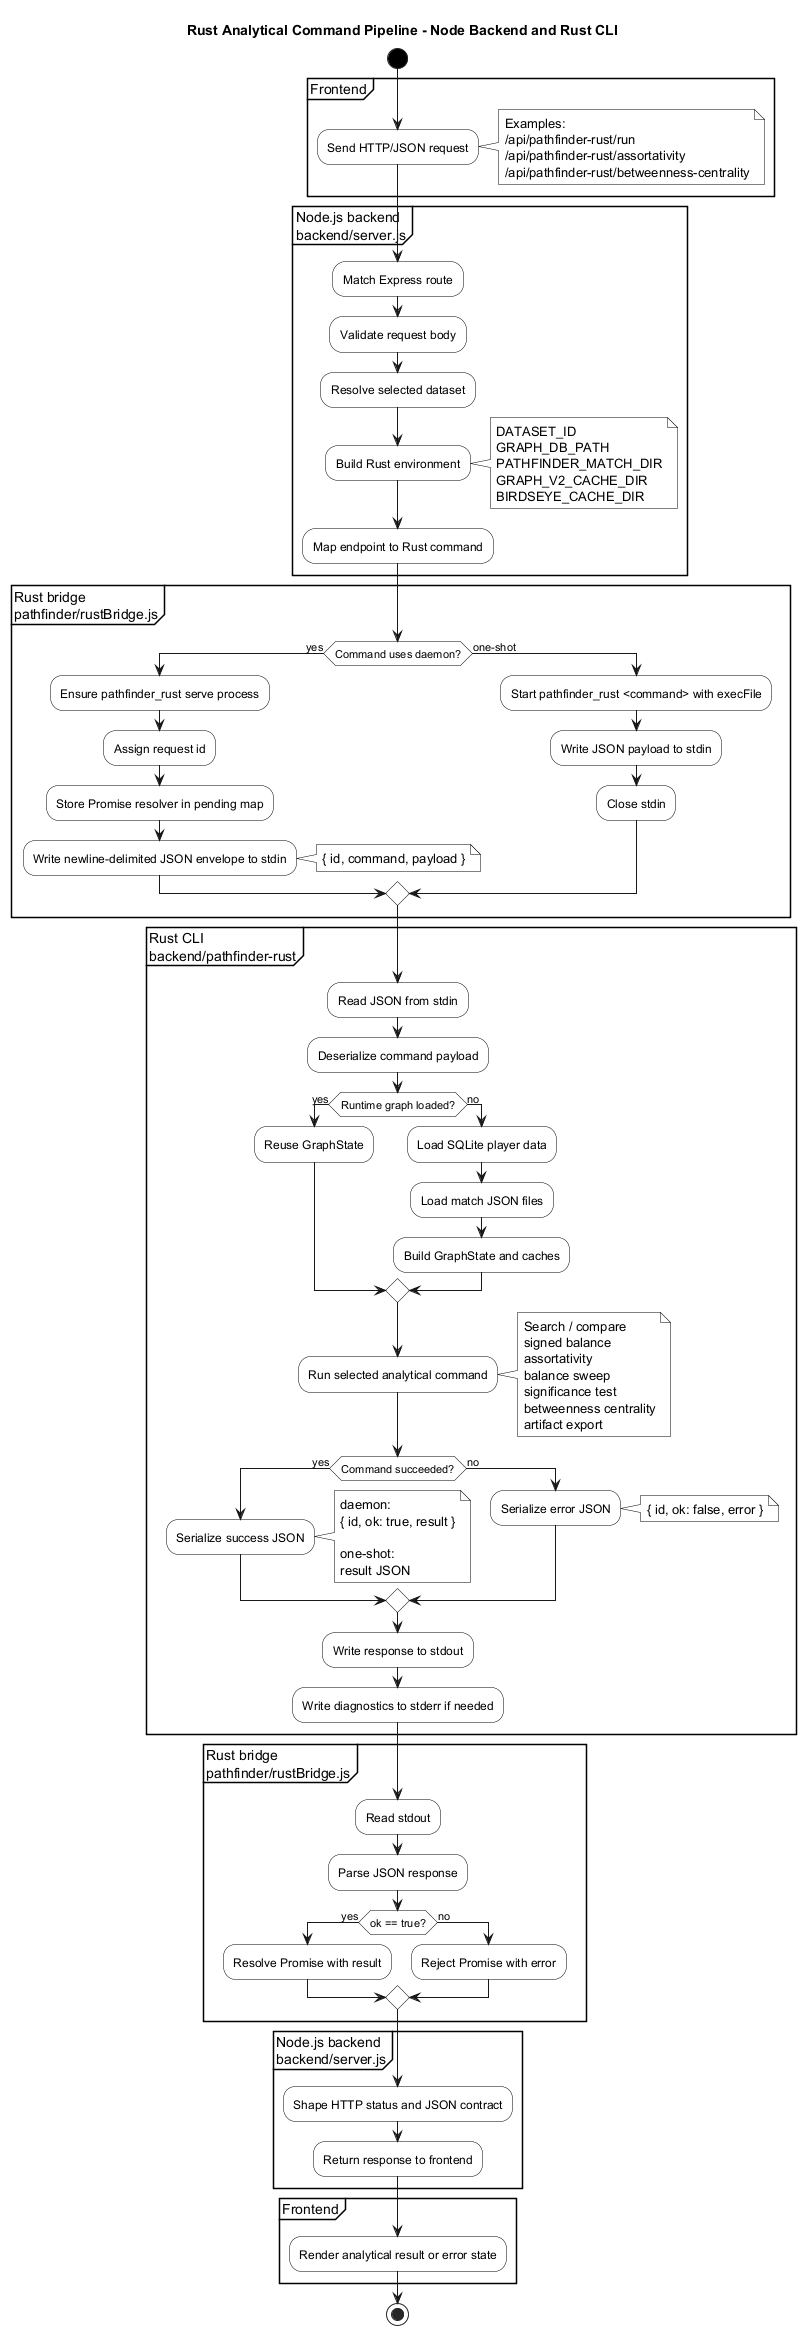
\includegraphics[width=0.98\textwidth,height=0.78\textheight,keepaspectratio]{rust-analytics-cli-pipeline.png}
\caption{A Node.js backend és a Rust CLI közötti parancsvezérelt kommunikáció sémája}
\label{fig:rust-analytics-command-flow}
\end{figure}

A Node/Express réteg a Rust számára nem konkurens implementáció, hanem vezérlő és integrációs héj. A fontosabb végpontok:

\begin{itemize}
    \item \texttt{GET /api/pathfinder-rust/options},
    \item \texttt{GET /api/pathfinder-rust/global-view},
    \item \texttt{GET /api/pathfinder-rust/engine-spec},
    \item \texttt{POST /api/pathfinder-rust/run},
    \item \texttt{POST /api/pathfinder-rust/compare},
    \item \texttt{POST /api/pathfinder-rust/player-focus},
    \item \texttt{POST /api/pathfinder-rust/signed-balance},
    \item \texttt{POST /api/pathfinder-rust/assortativity},
    \item \texttt{POST /api/pathfinder-rust/balance-sweep},
    \item \texttt{POST /api/pathfinder-rust/assortativity-significance}.
\end{itemize}

Ez a struktúra azért szerencsés, mert a frontend így stabil JSON-szerződéseken keresztül kommunikálhat a háttérréteggel, anélkül hogy tudnia kellene a belső gráfreprezentáció minden részletét.

A szerződésesség itt gyakorlati hasznot is hoz. A backend kezeli a datasetváltást, szükség esetén üríti a régi runtime-állapotot, átadja az aktuális útvonalakat a Rust motornak, és a frontend felé már csak a fogyasztható választ adja tovább. Ez csökkenti annak esélyét, hogy a frontend és a motor eltérő adatállapotra gondoljon ugyanabban a pillanatban.

\section{Strukturális egyensúly mint kísérleti analitika}

A \texttt{signed\_balance.rs} modul a többmeccses kapcsolatokat előjeles egyszerű gráffá projektálja. A fő döntések a következők:

\begin{itemize}
    \item pozitív él: domináns \texttt{ally} kapcsolat;
    \item negatív él: domináns \texttt{enemy} kapcsolat;
    \item támogatási küszöb: alapértelmezésben legalább 2 kapcsolat;
    \item döntetlen esetén: alapértelmezés szerint kizárás.
\end{itemize}

A modul teljesen géppel olvasható választ ad vissza, többek között:

\begin{itemize}
    \item a projektált gráf összefoglalóját,
    \item a kiegyensúlyozott és kiegyensúlyozatlan triádok számát,
    \item a triádtípusok eloszlását,
    \item példatriádokat,
    \item a legtöbb instabil triádban részt vevő játékosokat,
    \item opcionálisan klaszterszintű összegzést.
\end{itemize}

Ez a rész a rendszerben továbbra is megvalósított analitika, de nem a dolgozat egyik fő empirikus pillére. A formális projekció működik és reprodukálható; a korlát az, hogy az \texttt{enemyWeight} nem elég megbízható negatív társas kötés ahhoz, hogy a kapott arányokat erős szociális következtetésként kezeljem. Emiatt a modul a módszertani reflexió és a kísérleti diagnosztika része marad.

\section{Asszortativitás mint megvalósított analitika}

Az \texttt{assortativity.rs} modul a kiválasztott metrika és gráfmód mellett Pearson-korrelációt számol az élek két végpontja között, mindkét endpoint-orientációt figyelembe véve. A támogatott változók jelenleg:

\begin{itemize}
    \item \texttt{opscore},
    \item \texttt{feedscore},
    \item \texttt{social-path},
    \item \texttt{battle-path}.
\end{itemize}

A válasz nem csak egyetlen szám, hanem tartalmazza az analizált élmennyiséget, a kihagyások okait, a klaszteren belüli és klaszterek közötti bontást, valamint az erős és gyenge kapcsolatok szerinti bontást is. Ez kifejezetten erősíti a dolgozat védhetőségét, mert nem „díszanalitika”, hanem ellenőrizhető kimenet keletkezik.

Egy ilyen modul szakdolgozati értékét nem pusztán az adja, hogy „kiad egy korrelációt”, hanem az, hogy a kimenetben a mintaképzés is látható. A kihagyott élek, a hiányzó metrikák és a minimum match-count szabályok nélkül az asszortativitás sokkal kevésbé lenne védhető, mert nem lenne világos, milyen adatokon képződött az eredmény.

\section{A Graph V2 artifact-pipeline és a Rust motor összefüggése}

A Graph V2 pipeline egy specializált előre-generáló folyamat, amely a Rust motortól önállóan is futtatható és a böngészőnek fogyasztható artifact-csomagot állít elő. A Graph V2 kimenetei:

\begin{itemize}
    \item \texttt{manifest.json}: a teljes artifaktum metaadatai (matchCount, nodeCount, edgeCount, generationMs);
    \item \texttt{node\_meta.json}: csomópontszintű metaadatok;
    \item \texttt{node\_metrics.u32}: tömörített numerikus csomóponti mutatók bináris formátumban;
    \item \texttt{edge\_pairs.u32}: él-végpontpárok tömbje;
    \item \texttt{edge\_props.u32}: élhez tartozó kódolt tulajdonságok (ally/enemy jelzés, súly);
    \item \texttt{cluster\_meta.json}: klaszterszintű leíró adatok, orbitScore, orbitRadius, bridge-jelzők;
    \item \texttt{summary.md}: emberi és gépi olvasásra egyaránt alkalmas összegző fájl.
\end{itemize}

A Graph V2 és a fő Rust runtime gráfállapota (\texttt{GraphState}) szándékosan szétválasztott: a Graph V2 előre kiszámított, determinisztikus exportra optimalizált, a \texttt{GraphState} futásidejű útvonalkeresésre és kutatási analitikára. Ez teszi lehetővé, hogy ugyanabból a datasetből a böngésző statikus, gyors renderingre alkalmas artifaktumot kapjon, miközben az asszortativitás, a központiság és a kísérleti signed-balance parancsok futásidőben, a teljes gráfra futnak.

A Graph V2 clusteringAlgorithmVersion (\texttt{bounded-ally-groups-v2}) egy 20-as maximális csoportméretre korlátozott, ally-bizonyíték alapú klaszterezési algoritmus. Ez különbözik a Python-oldali moduláris klaszterezéstől: nem a teljes gráf modularitásmaximalizálására törekszik, hanem vizualizálhatóan kezelhető méretű, ally-centrikus csoportokat határol el. A két klaszterezési megközelítés együttes jelenléte a rendszerben nem redundáns, hanem különböző célokat szolgál.

\section{Kísérleti futtatók és robusztusság}

A Rust rétegben külön parancs és backend-végpont létezik az asszortativitás randomizációs szignifikanciatesztjéhez, valamint a signed-balance érzékenységvizsgálathoz. Ezek létezése azért fontos, mert a projekt nem áll meg az első leíró számnál, hanem támogatja a robusztussági és nullmodell-szerű összehasonlításokat is. A dolgozatban ezt úgy kezelem, mint kutatási infrastruktúrát: az asszortativitás központi eredmény, a signed-balance pedig azt dokumentálja, hol húzódik az előjeles projekció értelmezési határa.

% ===== chapters/13-pathfinder-lab-es-algoritmus-osszehasonlitas.tex =====
\chapter{Pathfinder Lab és algoritmus-összehasonlítás}

\section{A Pathfinder Lab szerepe a teljes rendszerben}

A Pathfinder Lab a projekt egyik legfontosabb ``átfordító'' modulja: itt válik a gráf a felhasználó számára nem csak megtekinthető hálózattá, hanem bejárható, kérdezhető kapcsolati térré. A lab célja nem pusztán az, hogy két játékos között egy útvonalat megjelenítsen, hanem az, hogy algoritmusonként is láthatóvá tegye, mit jelent ugyanaz a keresési feladat eltérő számítási szemléletekkel megoldani.

Ez szakdolgozati szempontból különösen értékes, mert a vizualizáció és az algoritmika itt közvetlenül találkozik. A hallgató vagy a bíráló nem csak egy képletet vagy egy táblázatot lát, hanem egy olyan felületet, amely mögött világos gráfelméleti és rendszerszintű döntések vannak.

\section{A támogatott algoritmusok összehasonlítási logikája}

A jelenlegi rendszerben négy algoritmus érhető el összevethető módon: BFS, Dijkstra, kétirányú keresés és A*. Ezek ugyanarra a problémaosztályra adnak választ, de eltérő feltételezésekkel:

\begin{table}[H]
\centering
\caption{A Pathfinder Labban szereplő algoritmusok összevetése}
\begin{tabularx}{\textwidth}{>{\raggedright\arraybackslash}p{2.8cm} >{\raggedright\arraybackslash}p{2.8cm} X}
\toprule
\textbf{Algoritmus} & \textbf{Mikor természetes?} & \textbf{Megjegyzés a projektben} \\
\midrule
BFS & súlyozatlan legrövidebb út & Jó baseline, könnyen magyarázható \\
Dijkstra & súlyozott utak & Referenciaalgoritmus a költség-alapú módokban \\
Kétirányú keresés & nagyobb gráf, kevésbé irányított keresés & Gyakorlati gyorsítás bizonyos esetekben \\
A* & jól kialakított alsó becsléssel & A projektben egzakt marad, nem csak vizuális heurisztika \\
\bottomrule
\end{tabularx}
\end{table}

A dolgozatban az összehasonlítás fő célja nem az, hogy ``győztest'' hirdessek, hanem az, hogy megmutassam: a rendszer képes ugyanazon gráfmodellt több algoritmikus nézőpontból kezelni, és a különbségek ellenőrizhetően visszakövethetők.

\begin{figure}[h]
\centering
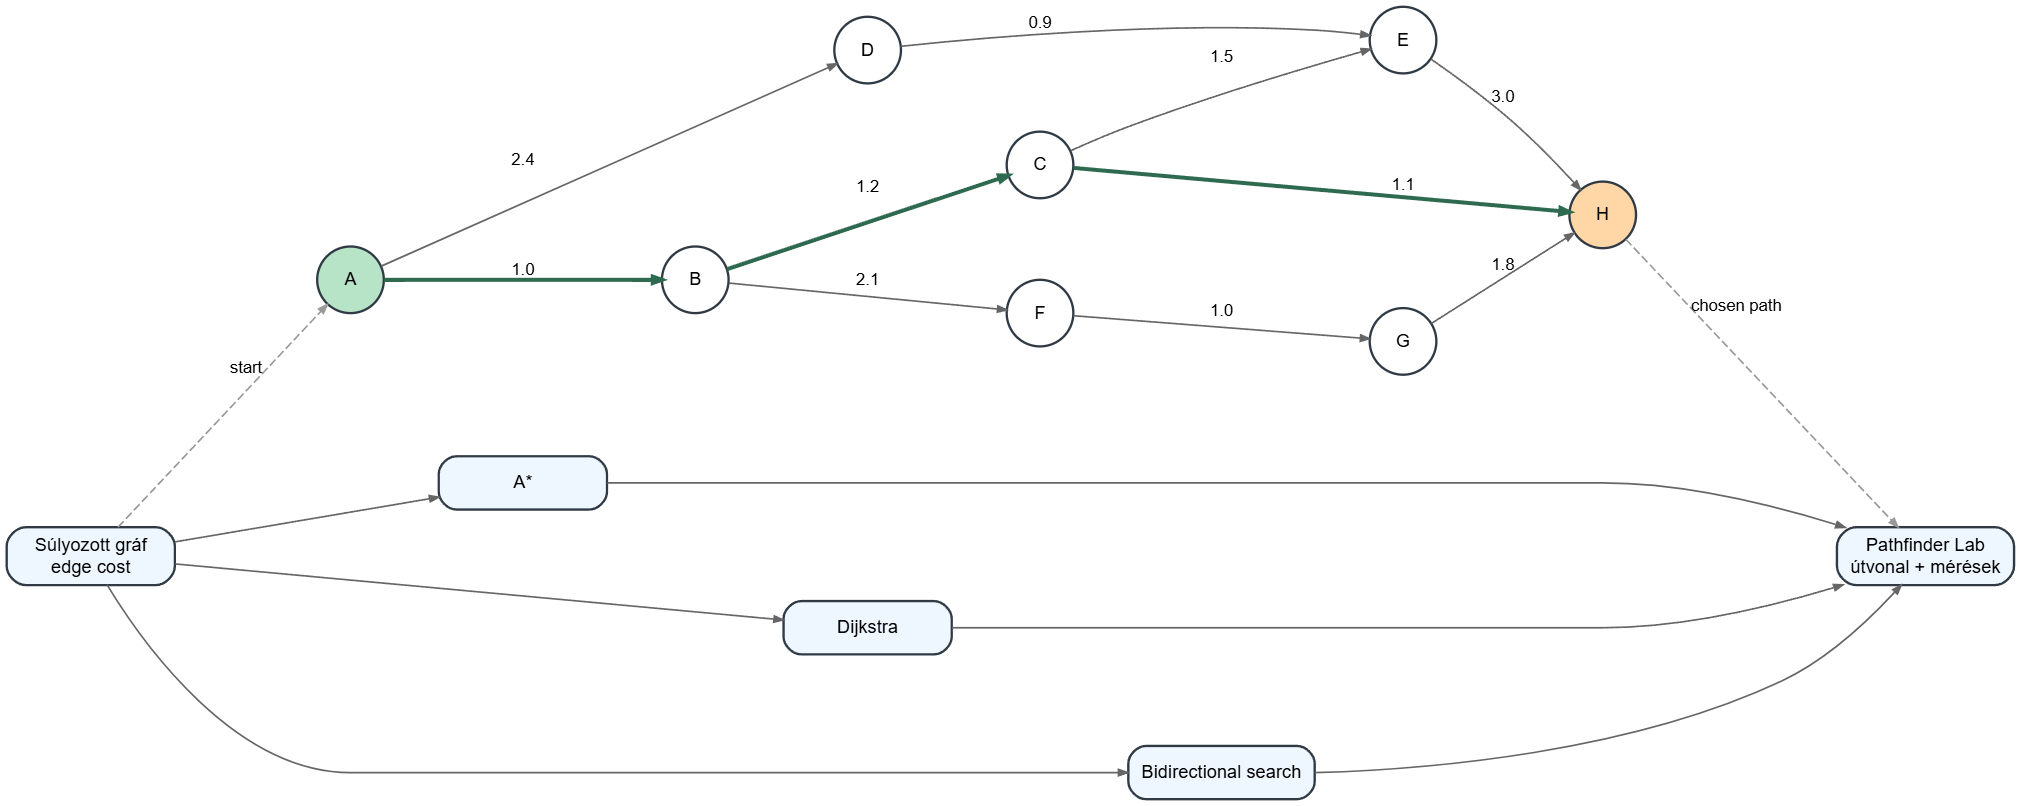
\includegraphics[width=0.92\textwidth]{assets/diagrams/thesis_pathfinding_graphviz.png}
\caption{A Pathfinder Lab algoritmikus értelmezése: ugyanazon súlyozott gráfon több keresési stratégia futtatható, majd az eredmény a replay és mérési rétegen keresztül válik összehasonlíthatóvá.}
\label{fig:pathfinder-graphviz-overview}
\end{figure}

\diagramfigure{A Pathfinder Lab és a frontend komponensstruktúrája - a keresési kérelmek útja a React nézettől a Rust motorig}{path finder and frontend component diagram.pdf}

\section{Kézi vezérlés, replay és magyarázhatóság}

A Pathfinder Lab egyik erőssége az, hogy a kimenetet nem feketedoboz-szerűen adja vissza. A replay panel és a vizuális léptetés lehetővé teszi, hogy a felhasználó:

\begin{itemize}
    \item megértse, milyen játékosokon megy keresztül az útvonal;
    \item lássa a gráfmód és a súlyozás hatását;
    \item összevesse az alternatív futtatásokat.
\end{itemize}

Ez a döntés oktatási és védhetőségi szempontból is hasznos. A rendszer nem elrejti az algoritmust, hanem láthatóvá teszi a döntési következményeket.

A \texttt{search.rs} alapján a replay mögött strukturált trace-adat áll. A motor minden releváns lépéshez képes rögzíteni az aktív csomópontot, a frontier rövidített állapotát, a meglátogatott csúcsok halmazát és a kiemelt éleket. Ezáltal a BFS, Dijkstra, kétirányú keresés és A* nem csak végső útvonal-hosszal hasonlítható össze, hanem a bejárási stratégia szintjén is. A magyarázhatóság tehát nem utólagos vizuális díszítés, hanem a keresőmotor válaszformátumának része.

\diagramfigure{A Pathfinder Lab replay panele - az útvonalösszegző, a léptetési vezérlők és a meglátogatott csomópontok statisztikái}{pathfinder-replay-panel.png}

\diagramfigure{Az overlay vezérlőpanel - szünet, sebesség és vizualizációs beállítások a replay lejátszás közben}{pathfinder_replay_overlay.png}

\section{Az algoritmusok részletes leírása}

\subsection{Szélességi keresés (BFS)}

A BFS az egyszerűbb esetekben természetes baseline: súlyozatlan módban garantáltan a minimális lépésszámú útvonalat adja, és a bejárás sorrendje teljesen meghatározott. A \texttt{search\_bfs()} implementáció egy FIFO-sort (\texttt{VecDeque}) tart fenn. Az algoritmus leáll, amint a célcsomópont először felbukkan a szomszédsági listán, ezáltal elkerülve felesleges kiterjesztést.

A trace-rögzítés szempontjából a BFS egyszerű, de informatív: minden ``expand'' és ``discover'' lépés rögzíthető, és az utólagos replay során jól látható, hogyan terjed ki a keresési határ egyenletesen minden irányban.

\diagramfigure{BFS futtatás a Pathfinder Labban - az egyenletes szélességi terjeszkedés és a minimális ugrásszámú útvonal jól látható a replay állapotban}{pathfinder-bfs-testrun.png}

\subsection{Dijkstra-algoritmus}

A Dijkstra-algoritmus \cite{dijkstra1959} binomiális kupac helyett bináris kupacot (\texttt{BinaryHeap}) használ, mert a Rust standard könyvtárban ez a beépített prioritásos sor. A \texttt{QueueState} struktúra lexikografikusan rendez: először az alacsonyabb \texttt{cost}, másodlagosan az alacsonyabb lexikográfiai csomópont-id szerint. Ez garantálja, hogy azonos súlyú utak esetén determinisztikusan mindig ugyanazt az útvonalat kapjuk.

A \texttt{traversal\_cost()} a kérésben megadott módnak megfelelően számít:

\begin{equation}
c(u,v) = \begin{cases}
1000 & \text{ha súlyozatlan mód} \\
\left\lceil 1000 / \max(1, w(u,v)) \right\rceil & \text{ha súlyozott mód}
\end{cases}
\end{equation}

A kapcsolaterősség ($w(u,v)$) social-path módban az \texttt{allyWeight}, battle-path módban a \texttt{total\_matches} érték. Az egységteszt (\texttt{dijkstra\_uses\_weighted\_costs\_to\_prefer\_stronger\_route}) ellenőrzi, hogy a súlyozott mód valóban a közvetett, de erős útvonalat preferálja a gyenge közvetlen éllel szemben.

\subsection{Kétirányú keresés}

A kétirányú BFS a forrásból és a célból párhuzamosan terjeszt ki egy-egy keresési frontot, és megáll, amint a két front találkozik. Az implementáció (\texttt{search\_bidirectional()}) felváltva bővíti a forrás-oldali és a cél-oldali sort (\texttt{expand\_frontier()}). A találkozási csomópont (\texttt{meeting\_node}) meghatározásakor az út az összefűzött forrás- és cél-részútvonalakból áll össze.

A kétirányú keresés elméleti előnye: sűrű vagy nagy gráfokban a meglátogatott csomópontok száma közelítőleg $O(\sqrt{n})$ lehet az egyirányú $O(n)$-hez képest, ha a gráf véletlenszerű. A project gráfján, ahol a komponensek erősen klaszteresek, a tényleges gyorsulás méréssel ellenőrizhető.

\subsection{A* keresés és heurisztika}

Az A* \cite{hart1968} algoritmus a Dijkstra-algoritmust terjeszti ki célirányos heurisztikával. Az \texttt{AStarState} struktúra a \texttt{path\_cost} (eddigi tényleges útvonalköltség) és a \texttt{heuristic\_cost} (célhoz vett alsó becslés) összegével rendez. A tie-breaking (\texttt{tie\_break\_distance}) egy másodlagos szempontot nyújt az azonos becsült összköltségű csomópontok közt.

A heurisztika (\texttt{heuristic\_lower\_bound()}) a \texttt{GraphState}-ben előre kiszámított \texttt{landmark\_distances} táblából és \texttt{cluster\_hops} adatból kombinál alsó becsléses értéket. Ez garantálja az elfogadhatóságot (admissibility): a heurisztika soha nem becsüli túl a valódi hátramaradó útvonalköltsége, ezért az A* helyes legrövidebb-utat ad.

Az egységtesztek minden releváns esetben igazolják, hogy az A* eredménye egyezik a Dijkstra-eredménnyel (\texttt{assert\_astar\_matches\_dijkstra}). Ez azt jelenti, hogy az A* nem vizuális gyorsítás, hanem valóban egzakt: csak a keresési sorrend más, az eredmény garantáltan azonos. Tesztelt esetek: súlyozatlan social-path, súlyozott social-path, battle-path, vegyes topológia, döntetlen-nehéz gráf, összekötetlen gráf, forrás==cél eset.

Különösen szemléletes az A* hatékonysága súlyozatlan módban: míg a BFS 5906 csomópontot látogat meg, az A* mindössze 60-at - mégis azonos 3-ugrás-os eredményt ad. A landmark heurisztika egyenesen a célhoz irányítja a keresést anélkül, hogy a teljes komponenst feltárná.

\diagramfigure{A* keresés súlyozatlan módban - mindössze 60 csomópontot látogat meg a BFS 5906-ával szemben, mégis azonos 3-ugrás-os eredményt ad; a heurisztika egyenesen a célba irányítja a keresést}{pathfinder-astar-unweighted-testrun.png}

\diagramfigure{A* keresés súlyozott módban - a landmark heurisztika és a klaszter-alapú alsó becslés relációs erősség mentén irányítja a bejárást}{pathfinder-astar-weighted-testrun.png}

\section{Kísérleti eredmény: strukturális távolság vs. relációs gerinc}

A Pathfinder Labban végzett tesztelés során az alábbi mérési eredmény különösen jelentős szakdolgozati szempontból:

\begin{table}[H]
\centering
\caption{BFS és súlyozott keresés összehasonlítása - ugyanazon játékospár, eltérő közelségi fogalmak}
\begin{tabularx}{\textwidth}{>{\raggedright\arraybackslash}p{3cm} >{\raggedright\arraybackslash}p{3cm} >{\raggedright\arraybackslash}p{2cm} X}
\toprule
\textbf{Algoritmus} & \textbf{Metrika} & \textbf{Eredmény} & \textbf{Értelmezés} \\
\midrule
BFS & Minimális ugrásszám & 3 & Legrövidebb szociális lánc \\
Dijkstra & Min. súlyozott költség & 8 & Legerősebb szövetségesi útvonal \\
A* & Min. súlyozott költség & 8 & Egyezik Dijkstrával ✓ \\
Kétirányú & Min. ugrásszám & 3 & Egyezik BFS-sel ✓ \\
\bottomrule
\end{tabularx}
\end{table}

A BFS által talált 3-ugrás-os útvonal strukturálisan létezik - de gyenge vagy egyszeri meccsből eredő kapcsolatokon halad át. A Dijkstra-algoritmus súlyozott módban elkerüli ezeket a gyenge kapcsolatokat, és helyette egy 8-ugrás-os útvonalat talál, amelyen minden él ismétlődő szövetségesi viszony. A két eredmény nem ellentmond egymásnak: két különböző közelségi fogalmat mér.

\subsection{Súlyozatlan vs. súlyozott: két különböző kutatási kérdés}

\textbf{Súlyozatlan mód (BFS, 3 ugrás) - strukturális távolság.} Hány kézfogás választja el a két játékost? Ez a szociális hálózatelemzés standard mérőszáma: Milgram \cite{milgram1967} ``hat fokos elválasztás'' kísérlete is ugrásos közelséget mért, nem kapcsolaterősséget. A 3-ugrás-os útvonal az eredeti gráf topológiájából fakad, és akkor is fennáll, ha az összekötő éleken egyszeri találkozás állt.

\textbf{Súlyozott mód (Dijkstra, 8 ugrás) - relációs gerinc.} Melyik a legerősebb szövetségesi lánc? A 8-ugrás-os útvonal minden éle teherbíró - ezek a játékosok ismételten együtt játszottak. A súlyozás a Flex Queue-ban kialakuló tényleges premade-szerkezetet tárja fel.

\subsection{Miért fontos az eltérés szakdolgozati szempontból?}

A BFS\,=\,3 / Dijkstra\,=\,8 divergencia önmagában is eredmény: megmutatja, hogy a gráf látszólagos összefüggésének mekkora hányada valódi ismétlődő kapcsolatokból, és mekkora hányada alkalmi meccsfelállításokból ered. A súlyozott legrövidebb út megkerüli az ``alkalmi szomszédság'' zajt, és a gráf sűrű magjára - a premade közösségre - irányítja a keresést.

Granovetter \cite{granovetter1973} gyenge kapcsolatok elvével is összefügg: a gyenge kapcsolatok (BFS útvonal) jobb információterjedési csatornák a gráfon keresztül, míg az erős kapcsolatok (Dijkstra út) határozzák meg a tényleges közösségi határokat. A premade csoportokat vizsgáló kutatásban a súlyozott út közvetlenül a premade-struktúrát ragadja meg.

\textbf{Egy mondatban:} A súlyozott legrövidebb út elemzés feltárja a Flex Queue hálózat relációs gerincét, és megkülönbözteti a strukturálisan elérhető játékosokat azoktól, akiket tartós együttjátszás köt össze - ez a különbség az ugrásos metrikák számára láthatatlan.

\diagramfigure{Az összes algoritmus futtatása súlyozatlan módban - BFS, Dijkstra, kétirányú és A* egységes összehasonlítása azonos játékospáron}{pathfinder-algocomparision-unweighted-test.png}

\diagramfigure{Az összes algoritmus futtatása súlyozott módban - Dijkstra és A* eltér a BFS és kétirányú keresés eredményétől; a heurisztikák csak súlyozott módban aktívak}{pathfinder-algocomparision-weighted-test.png}

\section{A gráfmód és a súlyozás együttes hatása}

A négy algoritmus két gráfmóddal és két súlyozási beállítással kombinálható. Ez $4 \times 2 \times 2 = 16$ lehetséges futtatási konfigurációt jelent, és mindegyik indokolt lehet más kutatási kérdésnél. A Pathfinder Lab ezt a dimenziót az interfészen keresztül elérhetővé teszi: a felhasználó láthatja, hogyan változik az útvonal és a bejárási stratégia, ha gráfmódot, súlyozást vagy algoritmust vált.

\begin{table}[H]
\centering
\caption{A négy algoritmus összehasonlítása a legfontosabb dimenziók mentén}
\begin{tabularx}{\textwidth}{>{\raggedright\arraybackslash}p{3cm} >{\raggedright\arraybackslash}p{2.5cm} >{\raggedright\arraybackslash}X >{\raggedright\arraybackslash}X}
\toprule
\textbf{Algoritmus} & \textbf{Optimális?} & \textbf{Memória} & \textbf{Fő erősség a projektben} \\
\midrule
BFS & Igen (súlyozatlan) & $O(n)$ & Egyszerű baseline, jól magyarázható replay \\
Dijkstra & Igen (súlyozott) & $O(n + m)$ & Referencia-algoritmus, lexikografikus döntetlen-kezelés \\
Kétirányú & Igen (súlyozatlan) & $O(n)$ & Potenciális gyorsulás klaszteres gráfon \\
A* & Igen (heurisztika elfogadható) & $O(n)$ & Célirányos bejárás, egzakt eredmény \\
\bottomrule
\end{tabularx}
\end{table}

\section{Miért fontos ez túl a UI-n?}

A Pathfinder Lab azért kap külön fejezetet, mert valójában nem frontend-extra. Ez az a réteg, ahol a Rust algoritmusok, a backend-szerződések, a perzisztens játékosprofilok és a böngészőben értelmezhető interakció egyetlen működő demonstrációvá állnak össze. Ha a dolgozat célja az, hogy az egész rendszer védhető legyen, akkor ezt a fejezetet nem lehet a vizuális melléklet szintjére leszorítani.

% ===== chapters/14-a-3d-bird-s-eye-sphere-es-globalis-halozati-vizualizacio.tex =====
\chapter{A 3D bird's-eye sphere és globális hálózati vizualizáció}

\section{A frontend szerepe}

A frontend jelenleg már nem egyetlen gráfnézet, hanem több, világosan elkülönített felületből álló mini-rendszer. Ez fontos minőségi ugrás a korábbi állapothoz képest, mert a projekt ekkor vált valóban bemutatható és narratívába rendezhető alkalmazássá.

A fő felületek:

\begin{itemize}
    \item \textbf{Match Analysis}: adatgyűjtési és mérkőzésellenőrző nézet,
    \item \textbf{Pathfinder Lab}: útvonalkeresési és algoritmus-összehasonlító nézet,
    \item \textbf{Full 3D Graph Sphere}: teljes hálózati madártávlat,
    \item \textbf{Assortativity}: teljesítmény-hasonlóságot vizsgáló analitikai oldal,
    \item \textbf{Betweenness Centrality}: Brandes-központisági és bridge/broker elemző oldal.
\end{itemize}

\section{Miért nem egyetlen képernyő?}

A felület több oldalra bontása nem esztétikai döntés volt, hanem használhatósági és védhetőségi kérdés. Egy szakdolgozati demo során sokkal könnyebb végigvezetni a nézőt azon az úton, hogy:

\begin{enumerate}
    \item adatot gyűjtünk vagy ellenőrzünk,
    \item gráfot és klasztereket generálunk,
    \item útvonalakat keresünk,
    \item globális struktúrát nézünk,
    \item kutatási jellegű elemzést futtatunk.
\end{enumerate}

Ha minden ugyanarra a képernyőre kerülne, a projekt inkább eszköztárnak, mintsem koherens rendszernek hatna.

\section{A 3D globális nézet}

A \emph{bird's-eye sphere} oldal a teljes hálózat vizuális áttekintésére szolgál. A legfontosabb tervezési döntés itt az volt, hogy a böngésző ne valós időben számolja a teljes layoutot, hanem a Rust réteg előre exportáljon minden fontos artifaktumot, és a frontend csak rendereljen.

Ennek több előnye van:

\begin{itemize}
    \item a layout determinisztikusabb,
    \item a demók megismételhetők,
    \item a böngésző terhelése kisebb,
    \item a vizuális réteg jobban elválik a számítási rétegtől.
\end{itemize}

\section{A bird's-eye manifest technikai tartalma}

Fontos különbséget tenni a teljes bird's-eye gömb-export és a Graph V2 artifact között. A bird's-eye gömb az összes látható játékost és élkapcsolatot rendereli bele a 3D térbe, míg a Graph V2 csak a minimum szövetségesi támaszú, klasztertagságú csomópontokat tárolja elemzésre alkalmas formában. A két struktúra ezért különböző csúcsszámot mutat ugyanarra a datasetre.

A \texttt{flexset} dataset esetében a Graph V2 artifact összefoglalója az alábbi adatokat rögzíti:

\begin{itemize}
    \item \textbf{5741} látható csúcs (klasztertagok és hozzájuk kapcsolódó csúcsok),
    \item \textbf{18\,548} látható él,
    \item \textbf{13\,572} ally-jellegű él (73.17\%),
    \item \textbf{4976} enemy-jellegű él (26.83\%),
    \item \textbf{1531} klasztercsoport,
    \item átlagos klaszterméret \textbf{3.750}, legnagyobb \textbf{20},
    \item generálási idő: \textbf{87\,472 ms}.
\end{itemize}

A \texttt{soloq} dataset Graph V2 artifaktuma:

\begin{itemize}
    \item \textbf{1538} látható csúcs,
    \item \textbf{4111} látható él,
    \item \textbf{2682} ally-jellegű él (65.24\%),
    \item \textbf{1429} enemy-jellegű él (34.76\%),
    \item \textbf{870} klasztercsoport,
    \item átlagos klaszterméret \textbf{1.768}, legnagyobb \textbf{20},
    \item generálási idő: \textbf{55\,674 ms}.
\end{itemize}

A két dataset ally/enemy arányának különbsége (flexset: 73/27, soloq: 65/35) szintén strukturálisan értelmes. A Flex Queue-ban a csapatonként öt fő játékstílus természetes módon dúsítja az ally-kapcsolatokat, míg a Solo/Duo Queue véletlenszerűbb csapatbeosztása az ellenfél-találkozások arányát növeli. Ez az arány önmagában is módszertani érv amellett, hogy a \texttt{flexset} erősebb asszociatív játékosgráfot hoz létre, de nem bizonyítja, hogy az enemy-élek negatív társas kötésekként értelmezhetők.

\section{A \texttt{flexset} mint asszociatív core-periphery játékosgráf}

A Graph V2 vizualizációt ebben a dolgozatban nem közvetlen barátsági vagy ellenségességi hálóként, hanem asszociatív játékosgráfként értelmezem. A csúcsok játékosokat, az élek pedig ismétlődő meccsbeli együtt- vagy szembekerülési bizonyítékot jelölnek. A legerősebb minta nem az előjeles egyensúly, hanem a core-periphery szerkezet: a központi régióban sok kereszt-klaszter szövetségesi kapcsolatot hordozó csoport jelenik meg, míg a külső gyűrűben sok kis, gyengén kapcsolt vagy teljesen híd nélküli lokális ally-csoport található.

A \texttt{flexset} artifactban \textbf{1531} bounded ally-csoport szerepel, ezek közül \textbf{815} bridge-jelölt klaszter, míg \textbf{716} külső pályára helyezett csoport nem rendelkezik cross-cluster ally híddal. A legfontosabb vizuális jel nem az, hogy egy klaszter balra vagy jobbra esik-e a képen, hanem a radiális pozíció: a kisebb orbit-radius erősebb hídjellegű, visszatérő ally-kapcsolatokra utal, a külső gyűrű pedig gyengén kapcsolt lokális szigeteket jelöl.

Ez az értelmezés módszertanilag erősebb, mint a signed-balance olvasat, mert nem igényli, hogy az ellenfélként való ismételt találkozást negatív társas kötésnek tekintsük. Elég hozzá az óvatosabb állítás: a Flex Queue match history ismétlődő asszociációs mintázatokat termel, amelyekben lokális ally-csoportok és hídgazdag központi régiók különülnek el.

A teljes rendszer bird's-eye gömb-exportja a backend által előre generált bináris és JSON artifaktumokat fogyaszt, és nem valós idejű számítást végez a böngészőben. Ez a tervezési döntés biztosítja, hogy a nagy gráfok megjelenítése is determinisztikus és reprodukálható maradjon.

A \texttt{server.js} és a bird's-eye exportútvonalak alapján a 3D nézet mögött több, külön felelősségű artifaktum áll. A frontend nem egyetlen nagy JSON-fájlt tölt be, hanem manifesztet és bináris tömböket fogyaszt.

\begin{table}[H]
\centering
\caption{A bird's-eye export fő artifaktumai}
\begin{tabularx}{\textwidth}{>{\raggedright\arraybackslash}p{4.2cm}X}
\toprule
\textbf{Fájl} & \textbf{Szerep} \\
\midrule
\texttt{manifest.json} & Metaadatok, darabszámok, skálázási és generálási információk \\
\texttt{node\_meta.json} & Csomópontszintű leíró metaadatok, frontend-hozzárendelések \\
\texttt{node\_positions.f32} & Lebegőpontos koordináták tömbje a gyors rendereléshez \\
\texttt{node\_metrics.u32} & Tömörített numerikus csomóponti mutatók \\
\texttt{edge\_pairs.u32} & Él-végpontpárok tömbje \\
\texttt{edge\_props.u32} & Élhez tartozó kódolt tulajdonságok \\
\bottomrule
\end{tabularx}
\end{table}

Ez a bontás rendszerszinten jól indokolható. A nagy tömegű numerikus adat bináris marad, ami gyorsabb böngészőoldali feldolgozást tesz lehetővé, miközben az emberileg olvasható metaadat külön JSON-rétegben marad. A frontend tehát megjelenít, nem pedig újraszámol.

\begin{figure}[H]
\centering
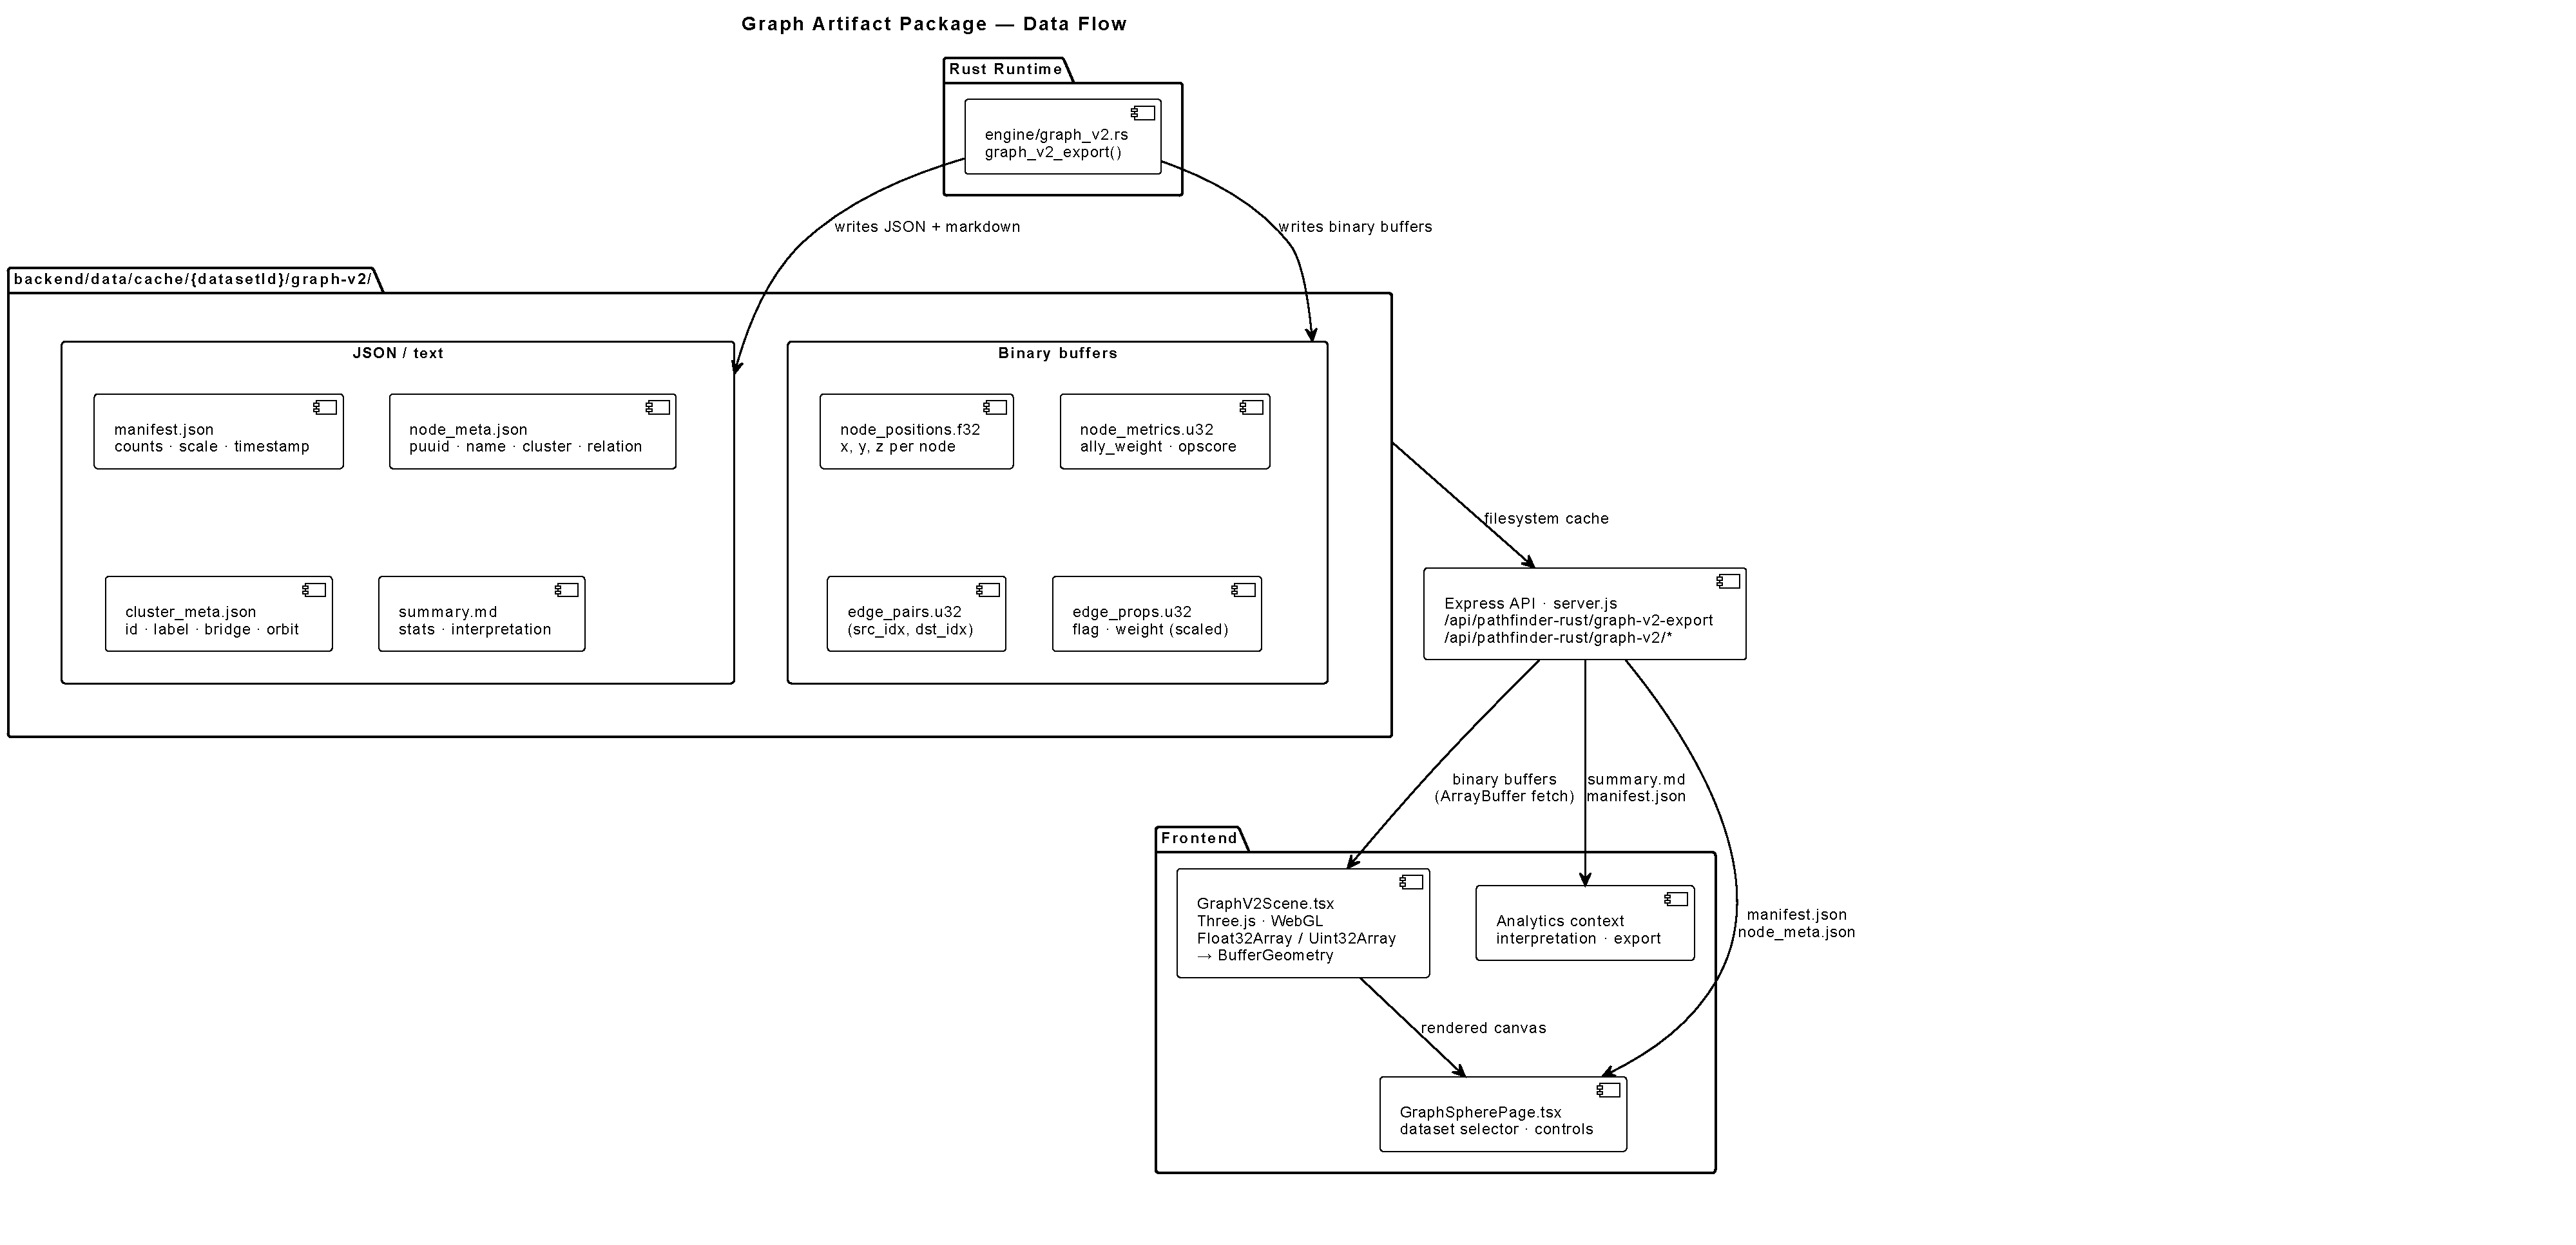
\includegraphics[width=0.95\textwidth,keepaspectratio]{graph artifact package dataflow.pdf}
\caption{A Graph V2 artifaktumcsomag adatfolyama: a Rust-exportőr bináris és JSON-rétegeket ír, az Express API kiszolgálja, a frontend WebGL-renderelőbe és elemzési kontextusba fogyasztja}
\end{figure}

\begin{figure}[H]
\centering
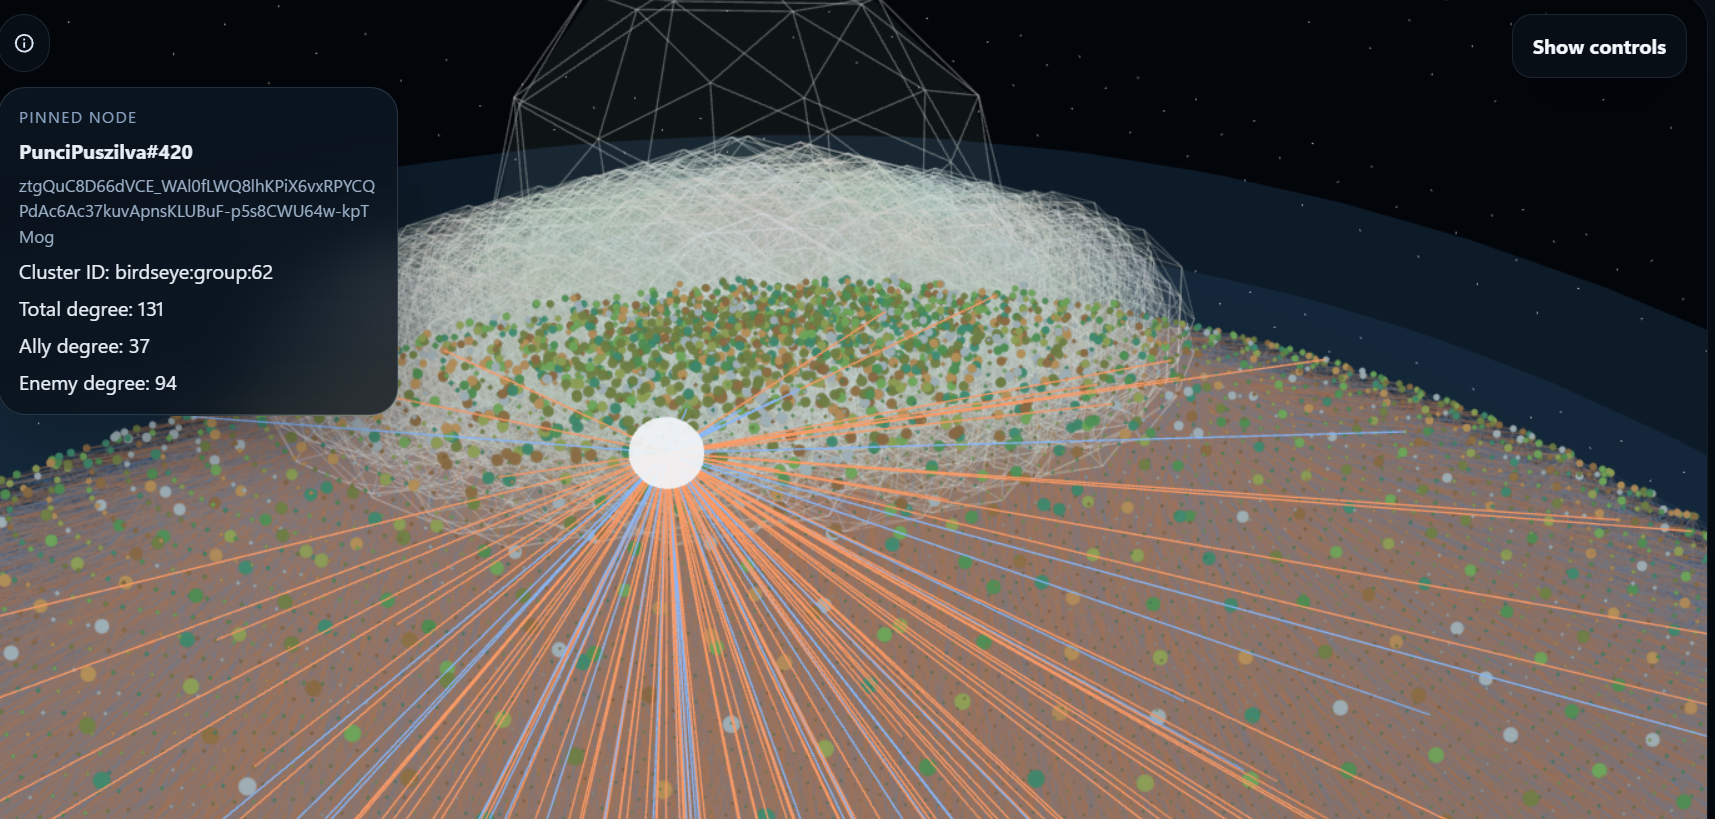
\includegraphics[width=0.98\textwidth,height=0.72\textheight,keepaspectratio]{birds-eye-cluster-view.png}
\caption{A teljes hálózat 3D madártávlati nézete az előre generált Rust-artifaktumokra építve}
\end{figure}

\begin{figure}[H]
\centering
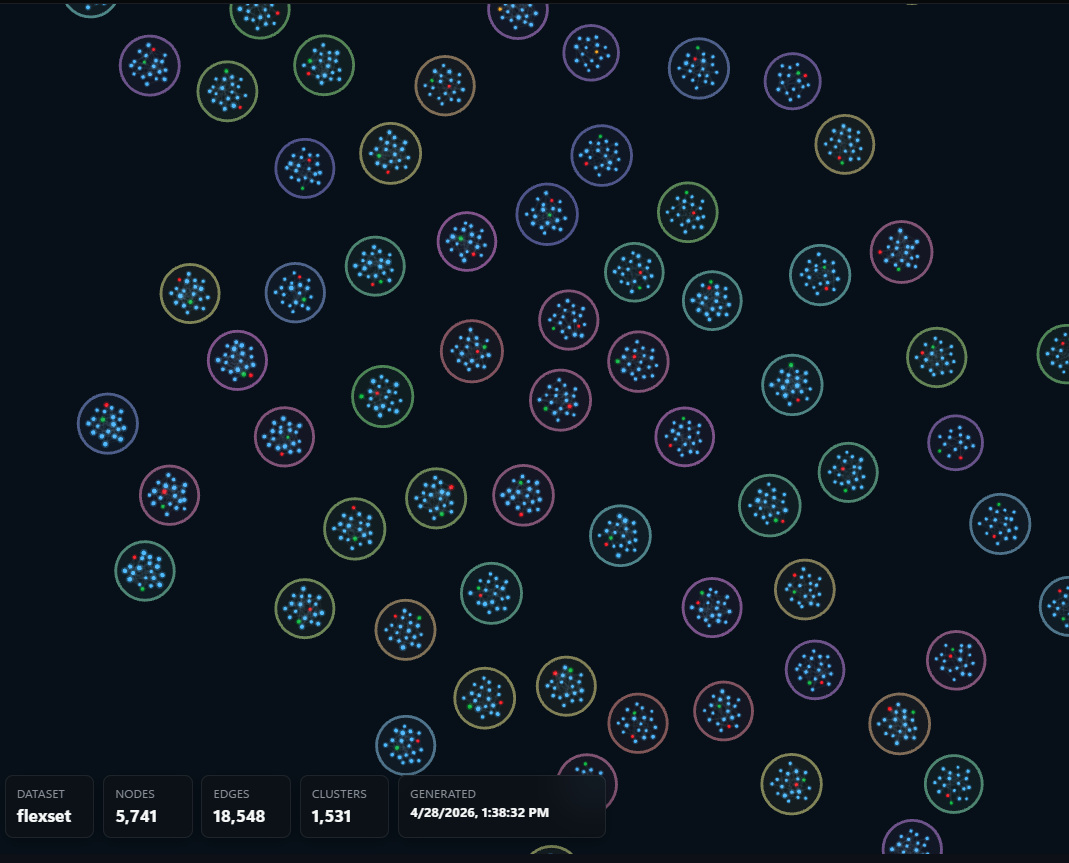
\includegraphics[width=0.98\textwidth,height=0.72\textheight,keepaspectratio]{flexset_associative_graph_clusters.png}
\caption{Sűrűbb klaszterfoltok és a térbeli elkülönítés a globális nézetben}
\end{figure}

\section{Pathfinder Lab}

A Pathfinder Lab az a felület, ahol a gráf nem elsősorban látványelemként, hanem algoritmikus térként jelenik meg. A felület támogatja:

\begin{itemize}
    \item forrás- és céljátékos kiválasztását,
    \item több algoritmus összehasonlítását,
    \item visszajátszási és léptetési funkciókat,
    \item súlyozott és nem súlyozott módot,
    \item többféle útvonalmód közötti váltást.
\end{itemize}

\section{Assortativity és központisági oldalak}

A kutatás-orientált frontend oldalak közös tulajdonsága, hogy nem elégednek meg egyetlen backend-válasz megjelenítésével. Az asszortativitási és központisági nézetek igyekeznek:

\begin{itemize}
    \item magyarázni a kontrollok jelentését,
    \item megmutatni a pipeline-összefüggéseket,
    \item elkerülni a túl gyors, túl erős társadalmi következtetéseket.
\end{itemize}

Ez különösen fontos, mert az ilyen típusú analitika könnyen félreértelmezhető. A felület ezért szándékosan tartalmaz interpretációs szövegeket és magyarázó elemeket is. A signed-balance oldal a jelenlegi dolgozati bemutatási útvonalból kikerült: a hozzá tartozó backend/Rust kód megmaradhat kísérleti opcióként, de a fő navigáció és a bemutatási útvonal már az asszortativitásra, a core-periphery gráfolvasatra és a Brandes-központiságra épül.

\section{Betweenness Centrality oldal}

A \texttt{BetweennessCentralityPage} a projekt egyik legkomplexebb analitikai nézetje. A felület nem pusztán indítja a Brandes-algoritmust, hanem eredményinterpretációs panelekkel, timing-összehasonlítással és döntési dokumentációval egészíti ki az analitikai kimenetet.

A oldal négy fő részből áll:

\begin{itemize}
    \item \textbf{Konfigurációs fejléc}: gráfmód (\texttt{battle-path} / \texttt{social-path}), él-súlyozás, minimum edge support és top-N korlát megadása; négy előre definiált preset (Strong 20, Medium 10, Wide 5, Full 1) gyors paraméterváltáshoz;
    \item \textbf{Projekcióolvasat}: a felület automatikusan értelmezi a megtartott él arányát - ha az arány 1\% alá esik, ``erős kötésű broker elemzés''; 10\% felett ``teljes gráf közelítő elemzés'';
    \item \textbf{Párhuzamossági összehasonlító}: ha a serial baseline futás engedélyezett, a felület megmutatja a serial és parallel futásidőt, a sebességarány-értékelést és a serial--parallel maximális abszolút eltérést (nulla kell legyen, ha a párhuzamosítás determinisztikus);
    \item \textbf{Broker-rangsor}: az első 6 csúcs kártyás nézete (rank, label, klasztercsoport, degree, strength, raw és normalizált BC), majd teljes táblázat.
\end{itemize}

A ``Dokumentált döntések'' panel (algorithm, parallelization, edge support rule, edge cost rule, normalization rule, graph scope) közvetlenül a Rust motor válaszából érkezik: a frontend nem rekonstruálja, hanem visszatükrözi az analitika által rögzített módszertani döntéseket. Ez azt jelenti, hogy a felületen megjelenő szöveges leírások mindig konzisztensek a tényleges futtatással.

Ez a nézet kulcsszerepet játszik a szakdolgozati bemutathatóság szempontjából: nem feketedoboz-eredményt ad vissza, hanem a futás körülményeivel, korlátaival és időbeli teljesítményével együtt prezentálja az eredményt.

\section{Player Detail oldal}

A \texttt{PlayerDetailPage} egy játékos-centrikus nézet, amely a kollektív analitikáktól eltérően egyetlen játékos profiljára fókuszál. Az oldal URL-paraméterrel (\texttt{?puuid=...}) adresszálható, így a Pathfinder Lab más nézeteiből közvetlenül lehet linkelni egy-egy csomópontra.

A nézet két fő részből áll: a játékoskereső mezőből (\texttt{PlayerLookupField}) és a \texttt{PlayerPerformanceCard} komponensből. Ez utóbbi összesíti az adott játékos pontszámait (opscore, feedscore), meccsadatait, szerepkör-eloszlását és klasztertagságát egy lapozás nélküli, pásztázható kártyanézetben.

Az oldal létjogosultsága a rendszerben az, hogy az aggregált elemzések (betweenness centralitás, asszortativitás, útvonalkeresési eredmények) sokszor néhány konkrét csomópontra irányítják a figyelmet. A Player Detail oldal lehetővé teszi, hogy ezek a csomópontok azonnal kontextusban is megvizsgálhatók legyenek, anélkül hogy az elemzőnek a nyers adatbázishoz kellene visszanyúlni.

\section{A Graph V2 artifaktum-pipeline részletei}
\label{sec:graph_v2_artifact}

A Graph V2 pipeline nem egyetlen monolitikus JSON-fájlt hoz létre, hanem egy gondosan megtervezett, kétféle formátumú (bináris és JSON) artifaktum-csomagot, amelyből a frontend oldalak és az analitikai motorok is hatékonyan tudnak táplálkozni.

\subsection{Az artifact-csomag összetétele}

A Graph V2 pipeline a \texttt{backend/data/cache/\{datasetId\}/graph-v2/} könyvtárba generálja a következő fájlokat:

\begin{itemize}
    \item \textbf{manifest.json}: metaadat és méretinformáció - meccszám, csúcsszám, élszám, generálási időbélyeg, verzió;
    \item \textbf{node\_meta.json}: csomópont-azonosítók és metaadatok - puuid, label, klaszterazonosító, pozíció (x, y), hídjelölő státusz;
    \item \textbf{node\_metrics.u32}: bináris, packed uint32 formátum - minden csomóponthoz sorrendben tárolja az opscore és feedscore értékeket egész skálán;
    \item \textbf{edge\_pairs.u32}: bináris élpárok - minden él két csomópont-indexeként tárolva;
    \item \textbf{edge\_props.u32}: bináris éltulajdonságok - allyWeight, enemyWeight, totalMatches minden élhez;
    \item \textbf{cluster\_meta.json}: klaszterszintű metaadatok - clusterID, memberCount, crossAllySupport, connectedAllyClusterCount, internalAllyEdges, orbitScore, orbitRadius, representative.
\end{itemize}

\begin{figure}[H]
\centering
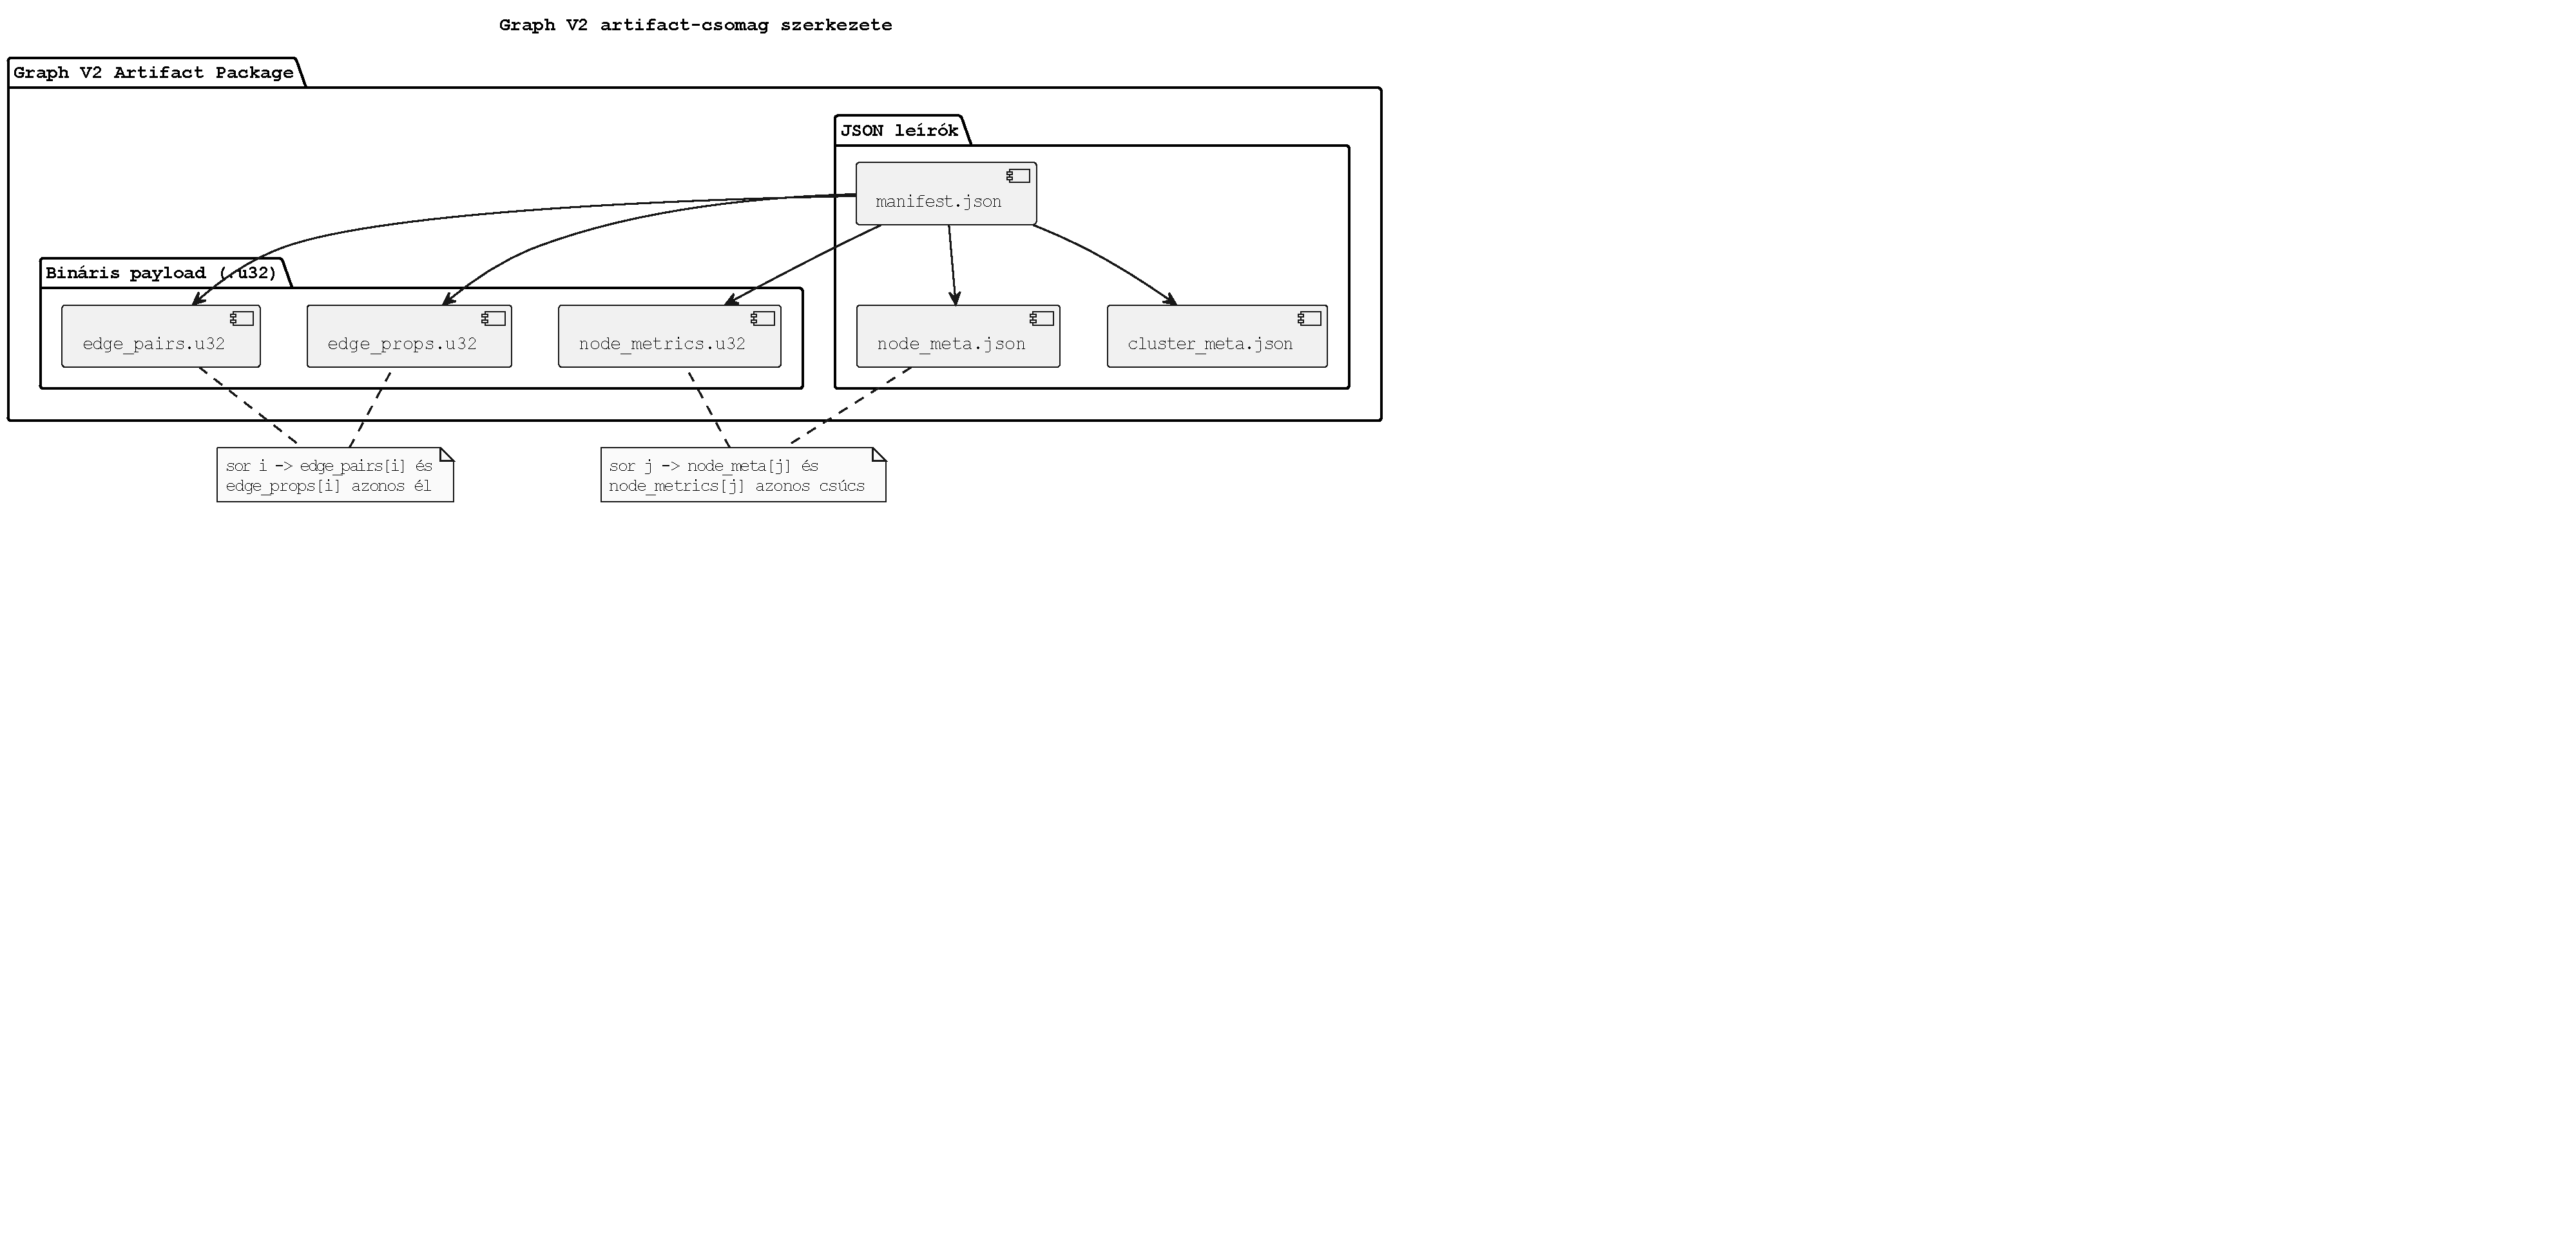
\includegraphics[width=\textwidth,height=0.82\textheight,keepaspectratio]{graph artifact components.pdf}
\caption{A Graph V2 pipeline bináris és JSON artifact-fájljainak szerkezete. A diagram a \texttt{graph-v2-artifact-structure.puml} forrás alapján különíti el a JSON leírókat (\texttt{manifest.json}, \texttt{node\_meta.json}, \texttt{cluster\_meta.json}) és a little-endian \texttt{.u32} bináris payloadokat (\texttt{edge\_pairs.u32}, \texttt{edge\_props.u32}, \texttt{node\_metrics.u32}). A \texttt{manifest.json} tartalmazza a csúcs-, él- és klaszterszámokat, míg a párhuzamos indexelés biztosítja, hogy az azonos sorszámú metadata- és metric-sor ugyanarra a csúcsra, illetve az azonos sorszámú edge-pair és edge-prop rekord ugyanarra az élre vonatkozzon.}
\end{figure}

A bináris formátumok (\texttt{.u32}) célja a betöltési teljesítmény: a frontend nem kénytelen JSON-parszolást végezni a csúcs- és élmutatókon; a bináris buffer közvetlenül beolvasható a WebGL renderelési pipeline-ba. Ez különösen a nagyméretű flexset esetén kritikus.

\subsection{A summary.md mint gépi és emberi kontextus}

Minden Graph V2 generálás után a pipeline létrehozza a \texttt{summary.md} fájlt, amely:

\begin{itemize}
    \item tartalmazza az összes kulcsmutatót (meccszám, csúcsszám, élszám, arányok, átlagos élsúly);
    \item dokumentálja a konstrukciós szemantikát (support-küszöb, tie-policy, klaszterméret-korlát);
    \item ML-szempontú feature-térképet biztosít a csomópont-, él- és klaszterszintű elemzési jelöltekhez;
    \item listázza a top bridge-orbit klasztereket;
    \item tartalmaz interpretációs korlátokat és javasolt elemzési irányokat.
\end{itemize}

Ennek a fájlnak kettős szerepe van: egyrészt fejlesztői ellenőrzőpontként működik (újragenerálásnál gyorsan ellenőrizhető, hogy a számok konzisztensek-e), másrészt gépi kontextusként is felhasználható - pontosan az a célba vett felhasználási mód, amelynek keretében a jelen dolgozat analitikai fejezetei is készültek.

\subsection{Verziókezelés és cache-érvénytelenítés}

A \texttt{graphBuilderVersion} mező (\texttt{graph-builder-v2.2}) explicit jelölője az artifaktum-csomag kompatibilitásának. Ha az algoritmus vagy a séma változik, a verzió frissítése egyértelműen jelzi, hogy a korábban generált artifact-csomagok nem felelnek meg az új elvárásoknak, és újra kell generálni azokat.

A \texttt{generatedAtUnixMs} Unix-időbélyeg lehetővé teszi a dataset-változás utáni automatikus érvénytelenítés detektálását: ha a meccs-JSON fájlok újabbak, mint a generálási időbélyeg, a rendszer tudja, hogy az artifact elavult.

\section{A backend API-szerződés}

A Rust motor és a frontend közötti kommunikáció a Node.js Express szerver (\texttt{backend/server.js}) által közvetített HTTP-végpontokon keresztül zajlik. A szerver nem saját maga végzi a számításokat, hanem a Rust folyamat stdin/stdout csatornáján továbbítja a kéréseket.

\subsection{Az aktuális főbb végpontok}

\begin{table}[H]
\centering
\caption{A backend API főbb végpontjai és szerepük}
\small
\begin{tabularx}{\textwidth}{>{\ttfamily\raggedright\arraybackslash}p{5.5cm} >{\raggedright\arraybackslash}X}
\toprule
\textbf{Végpont} & \textbf{Funkció} \\
\midrule
POST /api/pathfinder & Útvonalkeresési kérés (BFS/Dijkstra/A*/kétirányú) \\
POST /api/signed-balance & Kísérleti strukturális egyensúly-elemzés, nem fő felhasználói útvonal \\
POST /api/assortativity & Asszortativitás számítás \\
POST /api/betweenness-centrality & Brandes-betweenness futtatás \\
POST /api/balance-sweep & Kísérleti előjelprojekciós érzékenységi sweep \\
POST /api/assortativity-significance & Permutációs szignifikanciateszt \\
GET /api/graph-snapshot & Futásidejű gráfállapot-összefoglalás \\
GET /api/engine-spec & A Rust motor specifikációjának lekérése \\
GET /api/datasets & Elérhető datasetek listája \\
POST /api/switch-dataset & Dataset-váltás (Rust réteg újraindítással) \\
\bottomrule
\end{tabularx}
\normalsize
\end{table}

\subsection{Dataset-propagáció}

A dataset-váltás (\texttt{/api/switch-dataset}) nem csupán egy konfigurációs bit megváltoztatása. A Rust motor a dataset-specifikáció alapján teljes újraépítést végez: betölti az adott dataset meccs-JSON-jait, klasztereit és játékosprofilját, majd újraszámolja a landmark-távolságokat és a min-cost táblát. Ez az operáció jellemzően néhány másodpercig tart (a flexset esetén a futásidejű gráfépítés a teljes 4980 meccssel és 5741 csúccsal dolgozik).

Ez a közvetlen következménye annak az architektúrális döntésnek, hogy a Rust motor \emph{stateful}: nem minden kérésre, hanem beinduláskor (vagy dataset-váltáskor) tölti be a gráfot. Ez teljesítményi szempontból hasznos - nem kell minden egyes kérés előtt újraépíteni a gráfot -, de azt is jelenti, hogy a gráfállapot egy adott dataset-pillanathoz van kötve.

\subsection{A JSON-alapú kérés-válasz protokoll}

A Rust motor stdin-ről olvas egy JSON-objektumot (a kérés), majd stdout-ra ír egy JSON-objektumot (a válasz). A Node.js szerveroldal ezt a kommunikációt aszinkron Promisként kezeli. Ez a prototokol-tervzés egyszerű és debuggolható: a Rust motor tesztelható önállóan is, CLI eszközként, anélkül hogy a HTTP-szerver futna. A Node.js kizárólag a hálózati integrációért és a dataset-kezelésért felel.

% ===== chapters/15-a-strukturalis-egyensuly-mint-modszertani-hatareset.tex =====
\chapter{A strukturális egyensúly mint módszertani határeset}

\section{Miért került le a fő eredmények közül?}

A projektben elkészült signed-balance implementáció nem hibás algoritmus. A \texttt{signed\_balance.rs} modul determinisztikusan előállít egy előjeles egyszerű gráfot, teljesen összekapcsolt triádokat enumerál, majd a Heider--Cartwright--Harary-féle szabály szerint osztályozza őket. A visszaminősítés oka nem technikai, hanem szemantikai: a League of Legends matchmaking adataiban az ellenfélként való ismételt találkozás nem elég erős bizonyíték negatív társas kötésre.

Formálisan a projekció működik:

\begin{itemize}
    \item az \texttt{allyWeight} dominanciája pozitív élként kezelhető, mert a Flex Queue-ban a visszatérő csapattársi viszony részben szándékolt együttjátszást is tükrözhet;
    \item az \texttt{enemyWeight} dominanciája technikailag negatív élként jelölhető, de ez nem azonos ellenségességgel, rivalizálással vagy elutasítással;
    \item a döntetlen-kezelés, a minimum support és a triádenumerálás auditálható és újrafuttatható;
    \item a kapott arányok ezért inkább a választott projekció viselkedését mutatják, nem pedig bizonyított társas egyensúlyt.
\end{itemize}

\section{Az enemy-él szemantikai problémája}

A strukturális egyensúlyelmélet eredeti közege pozitív és negatív társas viszonyokra épül: barátságra, ellenszenvre, bizalomra, elutasításra vagy hasonló relációkra. A jelen projektben azonban egy enemy-él csak azt jelenti, hogy két játékos többször került egymással szembe, mint egy csapatba.

Ez sokféle okból történhet:

\begin{itemize}
    \item hasonló MMR-sávban játszanak;
    \item hasonló napszakban queue-znak;
    \item a Master$+$ Flex Queue aktív játékospoolja kicsi;
    \item a matchmaking ismételten ugyanazokat a játékosokat osztja ellenkező oldalra;
    \item a stabil premade-csoportok miatt a külső játékosok gyakrabban ellenfélként jelennek meg;
    \item az adatgyűjtési stratégia felerősítheti az ismétlődő találkozásokat.
\end{itemize}

Ezek közül egyik sem követeli meg, hogy a két játékos között negatív társas kapcsolat legyen. Ezért az \texttt{enemyWeight} negatív signed-network élként való kezelése túl erős állítás lenne a dolgozat fő empirikus narratívájához.

\section{Mit őriz meg a dolgozat?}

A signed-balance modul a repositoryban kísérleti opcióként megmaradhat, mert hasznos módszertani tanulságot ad: megmutatja, hogy egy formálisan elegáns gráfelméleti módszer hogyan válhat interpretációs szempontból gyengévé, ha az él szemantikája nem felel meg az elmélet előfeltevéseinek. A magas balance-ratio ezért legfeljebb óvatossági példaként használható: a szám lehet stabil a választott projekció alatt, de önmagában nem bizonyít társas harmóniát vagy strukturális stabilitást.

A dolgozati termékből és a fő frontend bemutatási útvonalból ezért kikerül a Signed Balance oldal és a kombinált Signed Balance + Assortativity futtató. A backend/Rust implementáció megtartható, de a dolgozat fő pillérei a következők:

\begin{itemize}
    \item a \texttt{flexset} asszociatív core-periphery játékosgráfként való értelmezése;
    \item a \texttt{flexset} és \texttt{soloq} datasetek kontrollált összehasonlítása;
    \item az \texttt{opscore} és \texttt{feedscore} asszortativitási eredményei;
    \item a Graph V2 konstrukciós és vizualizációs pipeline;
    \item a Rust útvonalkeresés és Brandes-betweenness központiság.
\end{itemize}

\section{Módszertani tanulság}

A visszaminősítés erősíti, nem gyengíti a dolgozatot. A dolgozat így nem azt állítja, hogy minden elegáns gráfelméleti modell automatikusan átültethető játékos-telemetriára, hanem azt, hogy az adatkeletkezési mechanizmust minden esetben össze kell vetni a választott modell előfeltevéseivel. A signed-balance esetben a formális számítás helyes, de a negatív él jelentése nem elég erős. Emiatt az elemzés határesetként marad: implementált, dokumentált, de nem fő bizonyíték.

% ===== chapters/16-asszortativitasi-elemzes.tex =====
\chapter{Asszortativitási elemzés}

\section{Az asszortativitás szerepe a dolgozatban}

Az asszortativitás azért lett külön kiemelt analitikai irány, mert egyszerre könnyen magyarázható és módszertanilag tiszta. A kérdés itt nem az, hogy ki ``jobb'' játékos, hanem az, hogy az összekapcsolt játékosok hajlamosak-e hasonló teljesítményprofilhoz tartozni.

A projektben ez különösen jó illeszkedés, mert a gráf és a játékosprofil már korábban is létezett. Nem kellett új, bizonytalan címkét bevezetni; elég volt a meglévő \texttt{opscore} és \texttt{feedscore} metrikákat a gráfél-végpontokra vetíteni.

\section{A számítási definíció}

A jelenlegi implementáció numerikus asszortativitást számol Pearson-korreláció formájában. Ha az él egyik végpontján mért értékeket $x_i$, a másik végpontén mért értékeket pedig $y_i$ jelöli, akkor az együttható a szokásos formában írható fel:

\begin{equation}
r = \frac{\sum_i (x_i-\bar{x})(y_i-\bar{y})}{\sqrt{\sum_i (x_i-\bar{x})^2}\sqrt{\sum_i (y_i-\bar{y})^2}}
\end{equation}

A projekt ezt két fontos kiterjesztéssel használja:

\begin{itemize}
    \item külön kezeli a \texttt{social-path} és \texttt{battle-path} gráfmódot;
    \item a globális együttható mellett külön bontásokat is képez klaszteren belüli, klaszterek közötti, illetve erős és gyenge kapcsolatok szerint.
\end{itemize}

A \texttt{backend/pathfinder-rust/src/engine/assortativity.rs} egyik lényeges technikai döntése, hogy az irányítatlan éleket mindkét endpoint-orientációval figyelembe veszi a Pearson-akkumulációban. Ez azért védhető, mert az élnek nincs természetes iránya, ugyanakkor a két végpont tulajdonságpárja szimmetrikusan járul hozzá a korrelációhoz. A modul emellett külön számlálja az alacsony támogatás, a hiányzó score és a túl rövid játékostörténet miatt kihagyott éleket is. Így az asszortativitási eredmény nem egy feketedoboz-korreláció, hanem egy jól dokumentált mintaképzési folyamat eredménye.

\begin{figure}[h]
\centering
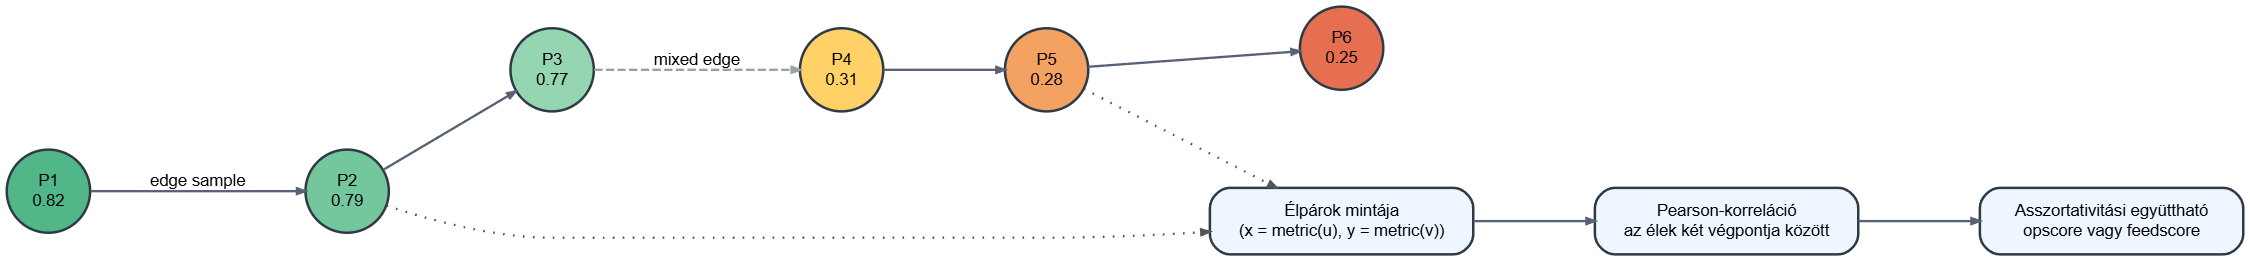
\includegraphics[width=0.92\textwidth]{assets/diagrams/thesis_assortativity_graphviz.png}
\caption{Az asszortativitás él-végponti értelmezése: az összekapcsolt játékospárok metrikaértékei Pearson-korrelációként kerülnek összesítésre.}
\label{fig:assortativity-graphviz-overview}
\end{figure}

\begin{figure}[H]
\centering
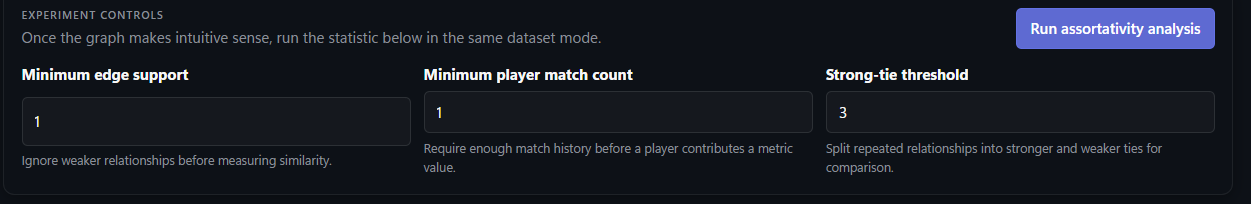
\includegraphics[width=0.98\textwidth,height=0.30\textheight,keepaspectratio]{assortavity-controls.png}
\caption{Az asszortativitási kísérlet frontend kontrolljai. A képen a minimum éltámogatás, a minimum játékos-meccsszám és az erős kapcsolat küszöbe látható; a bemutatott futtatásokban ezek rendre 1, 1 és 3 értékkel szerepelnek.}
\end{figure}

\begin{figure}[H]
\centering
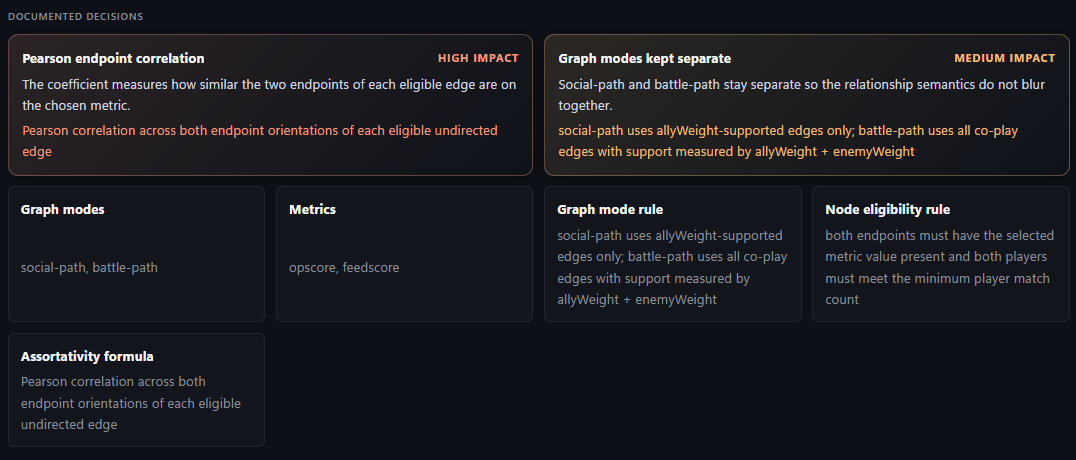
\includegraphics[width=0.98\textwidth,height=0.48\textheight,keepaspectratio]{assortavity-documented-desicions.png}
\caption{A frontend által megjelenített dokumentált módszertani döntések. A képernyő rögzíti, hogy Pearson endpoint-korrelációt használunk, a \texttt{social-path} és \texttt{battle-path} módokat külön kezeljük, a metrikák az \texttt{opscore} és \texttt{feedscore}, és csak azok a végpontok maradnak a mintában, amelyekhez érvényes metrika és elegendő meccstörténet tartozik.}
\end{figure}

\subsection{Él-végponti minta kiválasztása}

A Pearson-korreláció az élek között számítódik. Az asszortativitási implementáció az alábbiak szerint készíti elő az $(x_i, y_i)$ párokat:

\begin{enumerate}
    \item Az összes él végigmegy az aktuális gráfmódnak megfelelő szűrőn (social-path vagy battle-path).
    \item Minden élhez lekérdezésre kerül az egyik végpont score-ja (\texttt{opscore} vagy \texttt{feedscore}).
    \item Lekérdezésre kerül a másik végpont ugyanolyan score-ja.
    \item Ha bármelyik score hiányzik, vagy ha valamelyik játékos túl rövid játékostörténettel rendelkezik (\texttt{match\_count < minMatches}), az él kiesik.
    \item A maradék élek score-párjai a $(x_i, y_i)$ sor-párokkal képezik az akkumulált vektorokat.
\end{enumerate}

Ez a szűrés olyan mintahalmazt eredményez, amely az erős kapcsolatok körül tömörödik: ha egy él alacsony támogatás miatt nem tekinthető az elemzésre alkalmasnak, az kiesik az asszortativitás-számításból is. Ez módszertanilag erős, mert az asszortativitás nem egy ``mindent figyelembe vevő'' globális mérőszám, hanem a releváns kapcsolathálózat szerkezeti tulajdonsága.

\subsection{Gráfmód-specifikus él-súlyozás}

Az \texttt{edge\_support()} függvény a gráfmód alapján különbözően súlyozza az éleket:

\begin{equation}
w(u,v) = \begin{cases}
\texttt{ally\_weight} & \text{ha } \text{social-path} \\
\texttt{total\_matches} & \text{ha } \text{battle-path}
\end{cases}
\end{equation}

A social-path módban csak a szövetségesi kapcsolatok sugallják az él meglétét. A battle-path módban az összes ismétlődés (szövetséges és ellenséges) beszámít. Ez a különbség azt fejezi ki, hogy a két mód eltérő társas szerkezeti hipotéziseket tesztel:

- \textbf{Social-path}: ``A szövetségesi hálózatban a hasonló teljesítmények csoportosulnak?''
- \textbf{Battle-path}: ``Az összes ismétlődő kapcsolaton hasonló teljesítmények korrelálnak?''

Az asszortativitás e két módban eltérő értékeket mutat, mert a korrelálni kívánt edge-halmazok geometriai szerkezetileg különböznek.

\subsection{Klaszteren belüli és klaszterek közötti bontások}

Az implementáció nem csak globális korrelációt számol. Az eredmény az alábbi bontásokat is tartalmazza:

\begin{itemize}
    \item \textbf{Within-cluster}: csak az ugyanabban a klaszterben lévő csomópont-párokat tartalmazó élek;
    \item \textbf{Between-cluster}: az eltérő klaszterekbe tartozó végpontú élek;
    \item \textbf{Strong-tie}: magas support értékű élek (>= küszöb);
    \item \textbf{Weak-tie}: alacsony support értékű élek (< küszöb).
\end{itemize}

Ezek a bontások felvilágosítanak arról, hogy az asszortativitás a klaszteren belül vagy klaszterek között koncentrálódik-e. Ha a within-cluster érték magasabb, az azt jelzi, hogy az előre-klaszterezett csomópontok valóban hasonló score-ral rendelkeznek. Ha a between-cluster érték is magas, az azt mutatja, hogy az asszortativitás klaszter-független tulajdonság.

\subsection{Missing value policy}

A modul három lehetséges stratégiát támogat a hiányzó score-okkal szemben:

\begin{table}[H]
\centering
\caption{Hiányzó score-kezelési politikák}
\begin{tabular}{ll}
\toprule
\textbf{Politika} & \textbf{Hatás} \\
\midrule
\texttt{skip} & Az él kiesik az asszortativitás-számításból \\
\texttt{zero} & Az él meglétét 0.0-val helyettesíti \\
\texttt{mean} & Az él a dataset átlag-score-ját kapja \\
\bottomrule
\end{tabular}
\end{table}

Az alapértelmezett \texttt{skip} politika az óvatos választás: nem extrapolálunk hiányzó adatokra. Ezáltal az asszortativitás-érték az aktualista ``mit tudunk ténylegesen'' alapon számítódik, nem a feltételezéseken.

\section{Asszortativitási eredmények - flexset}

Az alábbi eredmények a percentilis-alapú \texttt{opscore}/\texttt{feedscore} értékeken alapulnak, amelyek az adatgyűjtés idején kerültek az adatbázisba (ld. \S\ref{sec:opscore_empirikus}). A következtetések ezen a modellen belül érvényesek.

A \texttt{flexset} dataseten elvégzett asszortativitási elemzés összesített eredményei:

\begin{table}[H]
\centering
\caption{Asszortativitás - \texttt{flexset}}
\begin{tabular}{llrr}
\toprule
\textbf{Gráfmód} & \textbf{Metrika} & \textbf{Korreláció} & \textbf{Mintaszám} \\
\midrule
\texttt{social-path} & \texttt{opscore} & 0.2346 & 61\,938 \\
\texttt{social-path} & \texttt{feedscore} & 0.1816 & 61\,938 \\
\texttt{battle-path} & \texttt{opscore} & 0.1461 & 179\,492 \\
\texttt{battle-path} & \texttt{feedscore} & $-0.0108$ & 179\,492 \\
\bottomrule
\end{tabular}
\end{table}

\begin{figure}[H]
\centering
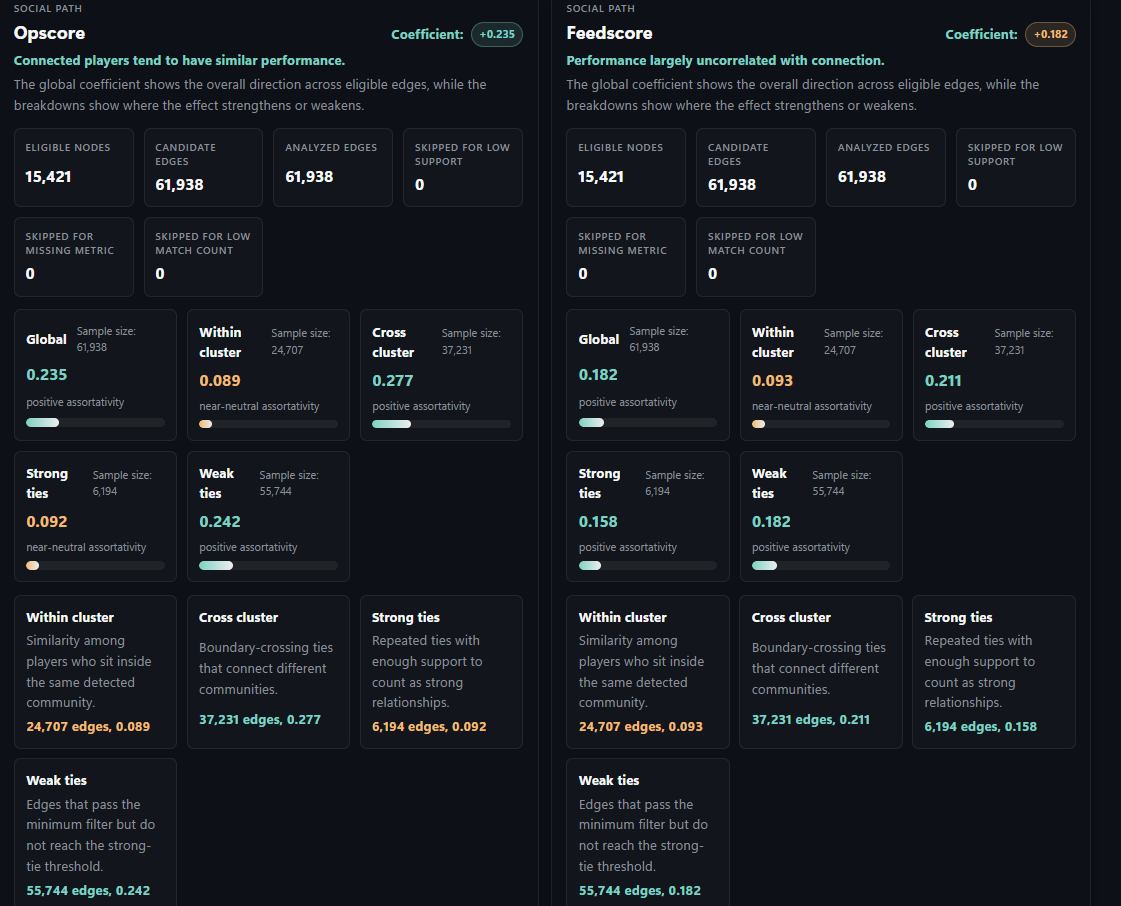
\includegraphics[width=0.98\textwidth,height=0.74\textheight,keepaspectratio]{f-assortavity-social-path-opfeedscore.png}
\caption{\texttt{flexset} social-path asszortativitás \texttt{opscore} és \texttt{feedscore} szerint. A képen 15\,421 jogosult csomópont és 61\,938 elemzett él szerepel; a globális együttható \texttt{opscore} esetén 0.235, \texttt{feedscore} esetén 0.182. A bontások azt mutatják, hogy a kereszt-klaszter élek erősebb pozitív jelet adnak, mint a klaszteren belüli élek, miközben a gyenge kapcsolatok nagy mintaszámmal hordozzák a pozitív mintázatot.}
\end{figure}

\begin{figure}[H]
\centering
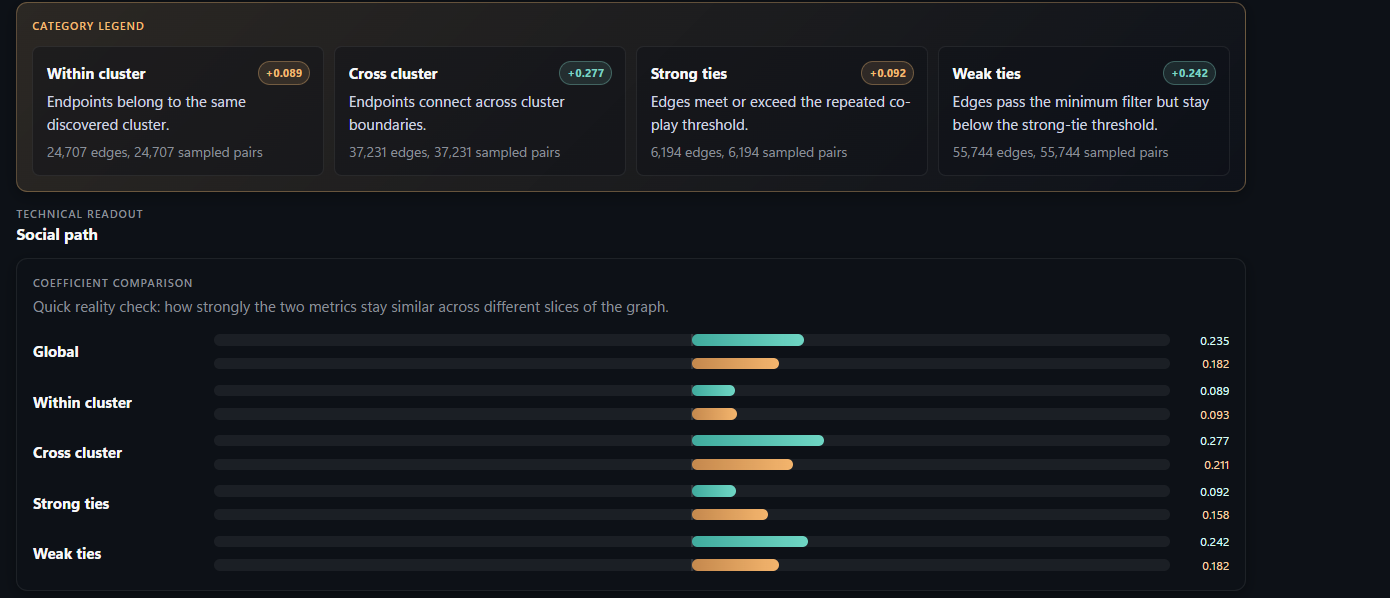
\includegraphics[width=0.98\textwidth,height=0.52\textheight,keepaspectratio]{f-assortavity-socialpath-readout.png}
\caption{\texttt{flexset} social-path technikai readout. A sávos összehasonlítás a globális, within-cluster, cross-cluster, strong-tie és weak-tie bontásokat teszi egymás mellé; látható, hogy az \texttt{opscore} minden bontásban pozitív, a \texttt{feedscore} pedig social-path módban szintén pozitív marad.}
\end{figure}

\begin{figure}[H]
\centering
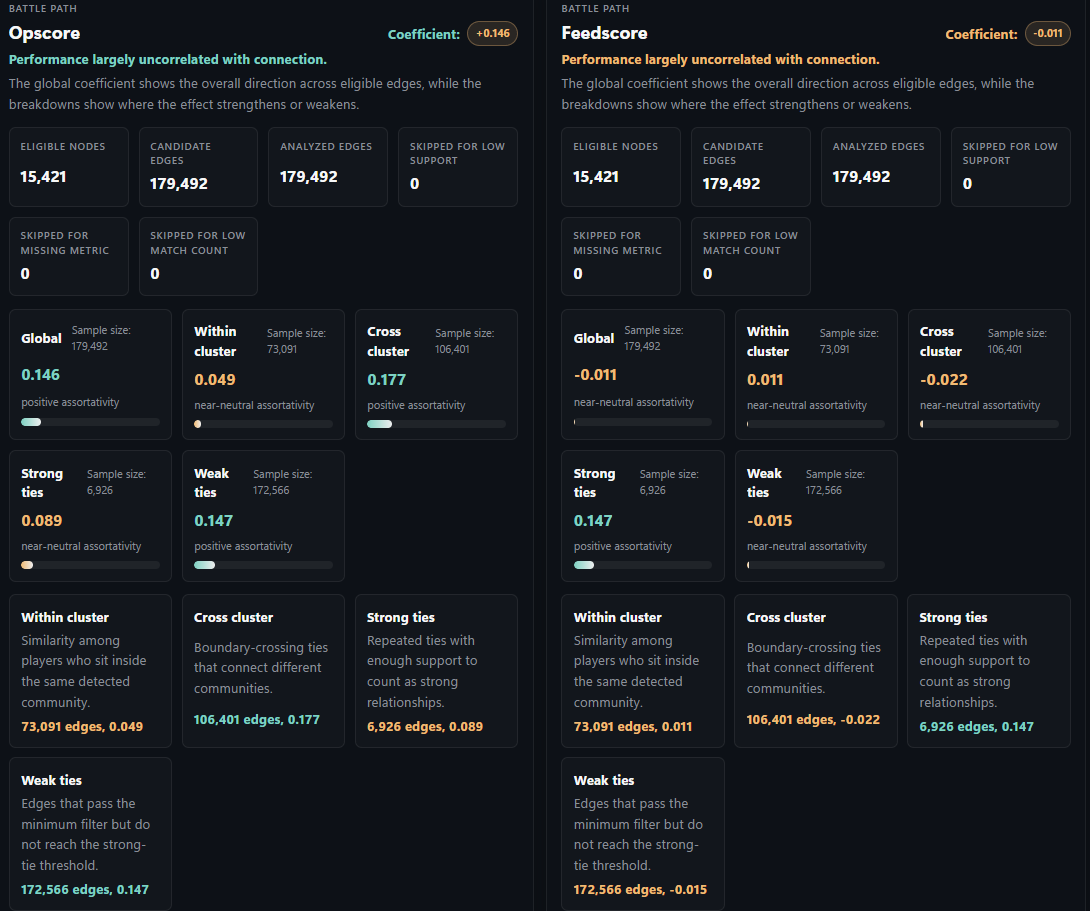
\includegraphics[width=0.98\textwidth,height=0.74\textheight,keepaspectratio]{f-assortavity-battle-path-opfeedscore.png}
\caption{\texttt{flexset} battle-path asszortativitás \texttt{opscore} és \texttt{feedscore} szerint. A képen ugyanaz a 15\,421 jogosult csomópont, de már 179\,492 elemzett él látható; a \texttt{battle-path} mód több kapcsolatot vesz be, ezért a \texttt{opscore} jel 0.146-ra gyengül, a \texttt{feedscore} pedig gyakorlatilag nullára esik ($-0.011$).}
\end{figure}

\begin{figure}[H]
\centering
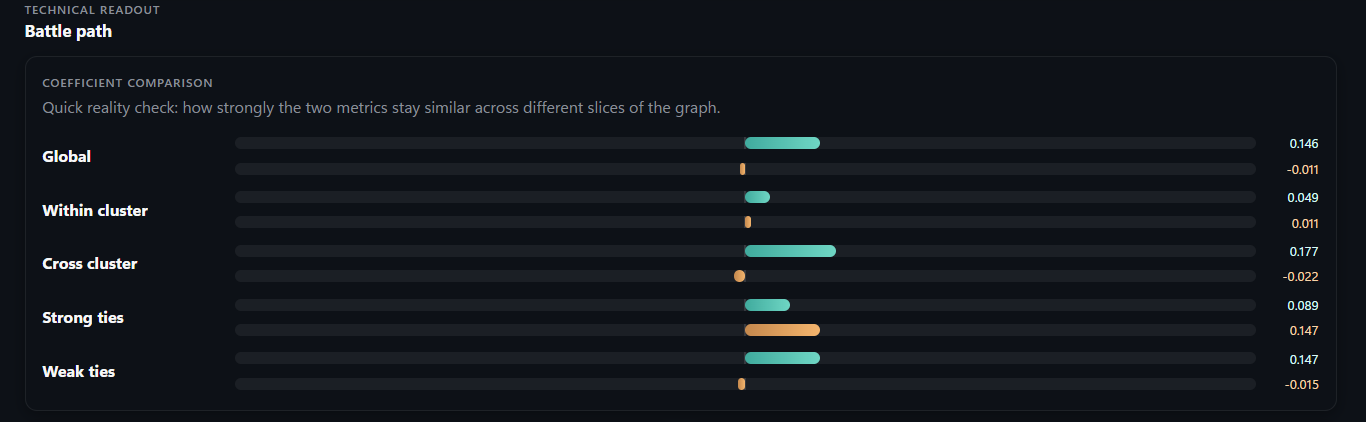
\includegraphics[width=0.98\textwidth,height=0.36\textheight,keepaspectratio]{f-assortavity-battlepath-readout.png}
\caption{\texttt{flexset} battle-path technikai readout. A képernyőn az látszik, hogy a battle-path \texttt{opscore} pozitív, de mérsékeltebb hasonlósági jelet ad, míg a \texttt{feedscore} globálisan és a gyenge kapcsolatokon közel nulla vagy enyhén negatív.}
\end{figure}

\begin{figure}[H]
\centering
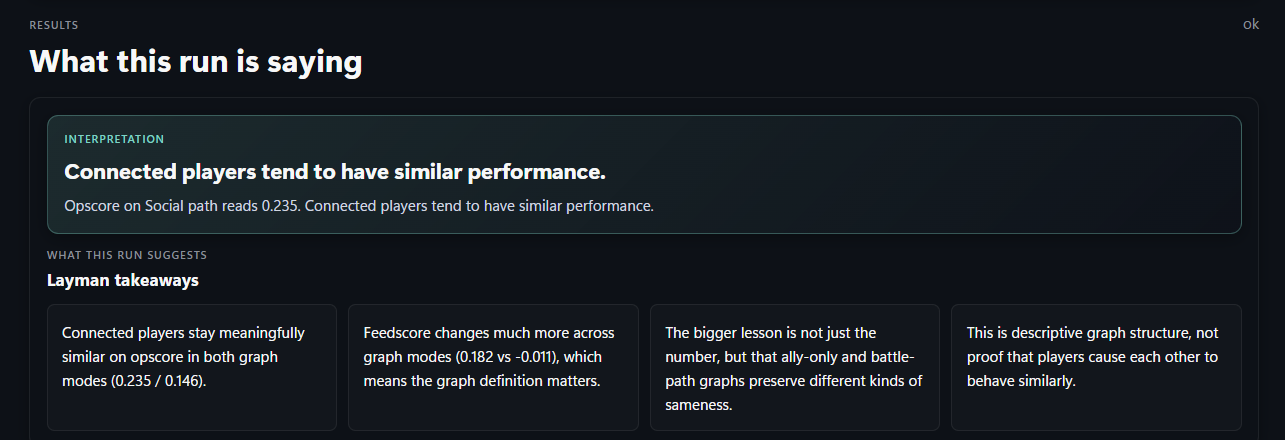
\includegraphics[width=0.98\textwidth,height=0.38\textheight,keepaspectratio]{f-assortavity-layman-takeaways.png}
\caption{\texttt{flexset} közérthető frontend-összegzés. A képernyő azt emeli ki, hogy a kapcsolt játékosok \texttt{opscore} szerint mindkét gráfmódban hasonlóbbak, a \texttt{feedscore} viszont erősen gráfmód-függő; a következtetés leíró hálózati szerkezetről szól, nem oksági vagy pszichológiai állításról.}
\end{figure}

A \texttt{flexset} eredményeinek legfontosabb tanulsága az, hogy a szövetségesi kapcsolatokra épülő social-path gráfban jelenik meg a legerősebb teljesítményhasonlósági jel. Ez illeszkedik ahhoz az értelmezéshez, hogy a Flex Queue nem pusztán véletlen matchmaking-minta: a visszatérő csapattársi kapcsolatok egy része olyan asszociatív szerkezetet ad, amelyben a hasonló \texttt{opscore}-ral rendelkező játékosok gyakrabban kapcsolódnak egymáshoz.

A bontások ugyanakkor finomítják ezt a képet. A \texttt{flexset} social-path képernyőn a cross-cluster \texttt{opscore} érték magasabb, mint a within-cluster érték. Ez arra utal, hogy a hasonló teljesítményprofil nem csak zárt, sűrű klasztereken belül jelenik meg, hanem klaszterhatárokon átívelő kapcsolatokon is. Emiatt az asszortativitás nem egyszerűen a klaszterezés mellékterméke: a határkapcsolatokban is mérhető, és ezért jól kiegészíti a core-periphery értelmezést.

\section{Asszortativitási eredmények - soloq}

A \texttt{soloq} dataseten ugyanolyan paraméterekkel:

\begin{table}[H]
\centering
\caption{Asszortativitás - \texttt{soloq}}
\begin{tabular}{llrr}
\toprule
\textbf{Gráfmód} & \textbf{Metrika} & \textbf{Korreláció} & \textbf{Mintaszám} \\
\midrule
\texttt{social-path} & \texttt{opscore} & 0.1750 & 37\,976 \\
\texttt{social-path} & \texttt{feedscore} & 0.1012 & 37\,976 \\
\texttt{battle-path} & \texttt{opscore} & 0.1625 & 84\,393 \\
\texttt{battle-path} & \texttt{feedscore} & $-0.0366$ & 84\,393 \\
\bottomrule
\end{tabular}
\end{table}

\begin{figure}[H]
\centering
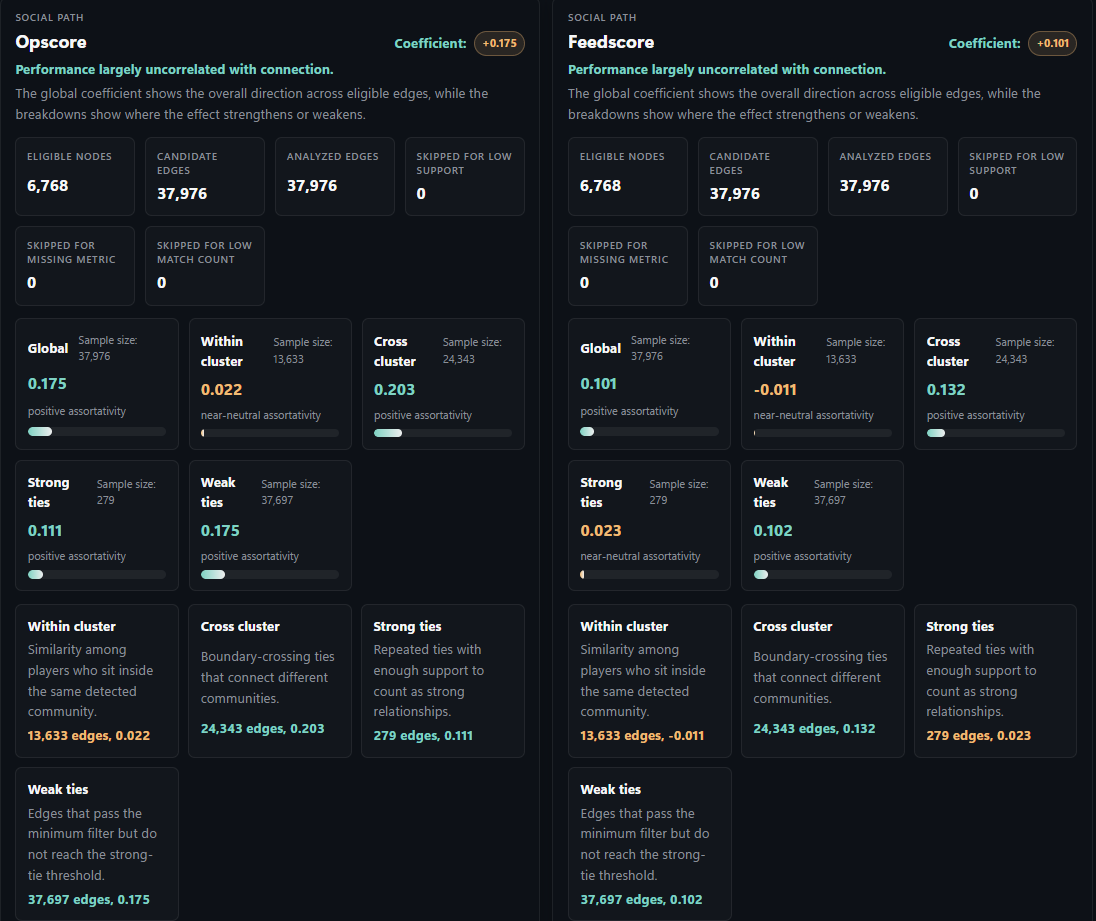
\includegraphics[width=0.98\textwidth,height=0.74\textheight,keepaspectratio]{sq-assortavity-social-path-opfeedscore.png}
\caption{\texttt{soloq} social-path asszortativitás \texttt{opscore} és \texttt{feedscore} szerint. A képen 6\,768 jogosult csomópont és 37\,976 elemzett él szerepel; a globális együttható \texttt{opscore} esetén 0.175, \texttt{feedscore} esetén 0.101. A pozitív értékek megmaradnak, de gyengébbek, mint a \texttt{flexset} social-path eredményei.}
\end{figure}

\begin{figure}[H]
\centering
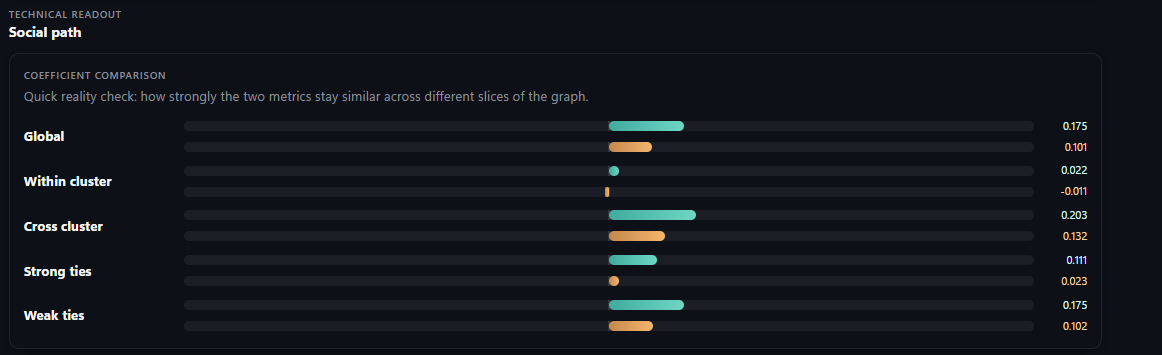
\includegraphics[width=0.98\textwidth,height=0.36\textheight,keepaspectratio]{sq-assortavity-socialpath-readout.png}
\caption{\texttt{soloq} social-path technikai readout. A sávos nézet azt mutatja, hogy a cross-cluster bontás adja a legerősebb pozitív jelet, míg a within-cluster értékek közel semlegesek; a strong-tie minta különösen kicsi, ezért ebben a datasetben óvatosan értelmezendő.}
\end{figure}

\begin{figure}[H]
\centering
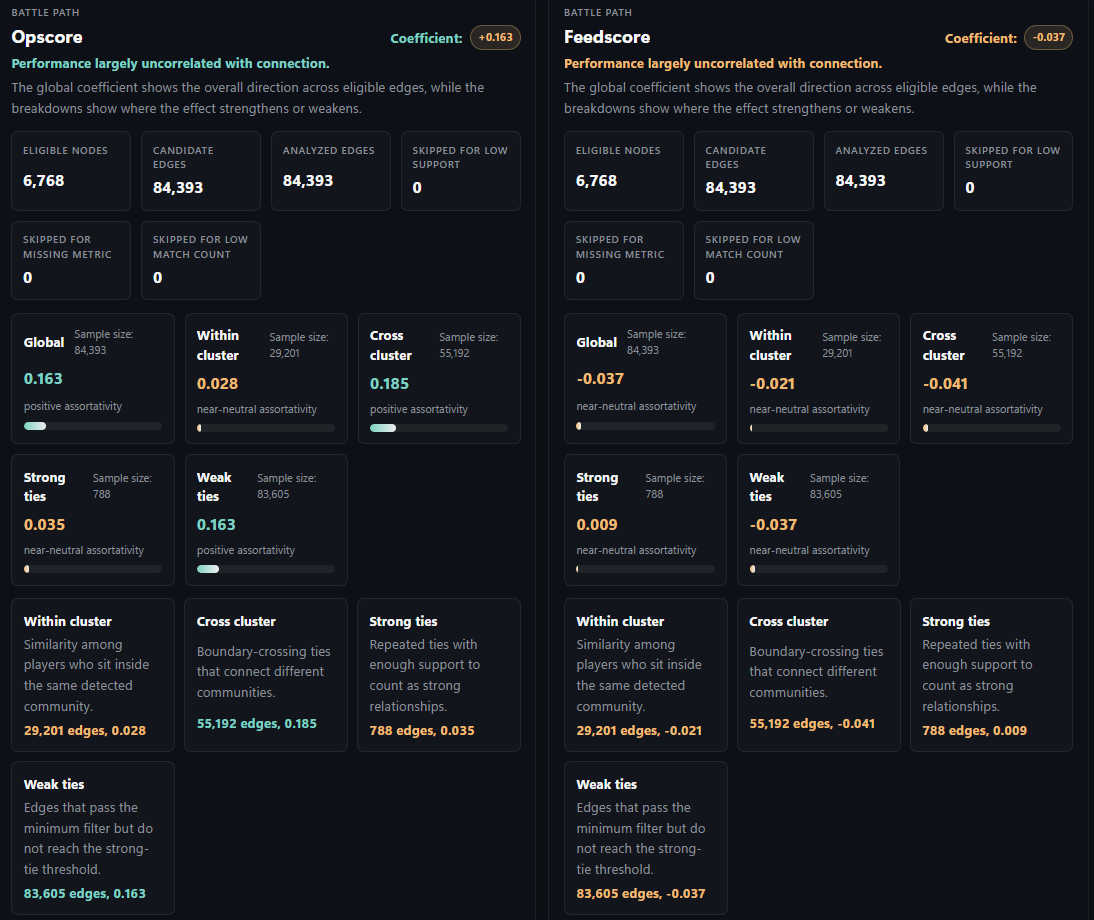
\includegraphics[width=0.98\textwidth,height=0.74\textheight,keepaspectratio]{sq-assortavity-battle-path-opfeedscore.png}
\caption{\texttt{soloq} battle-path asszortativitás \texttt{opscore} és \texttt{feedscore} szerint. A képen 84\,393 elemzett él látható; az \texttt{opscore} globálisan 0.163 marad, a \texttt{feedscore} viszont $-0.037$ értékre fordul, ami gyakorlatilag kapcsolat nélküli vagy enyhén ellentétes mintázatot jelez.}
\end{figure}

\begin{figure}[H]
\centering
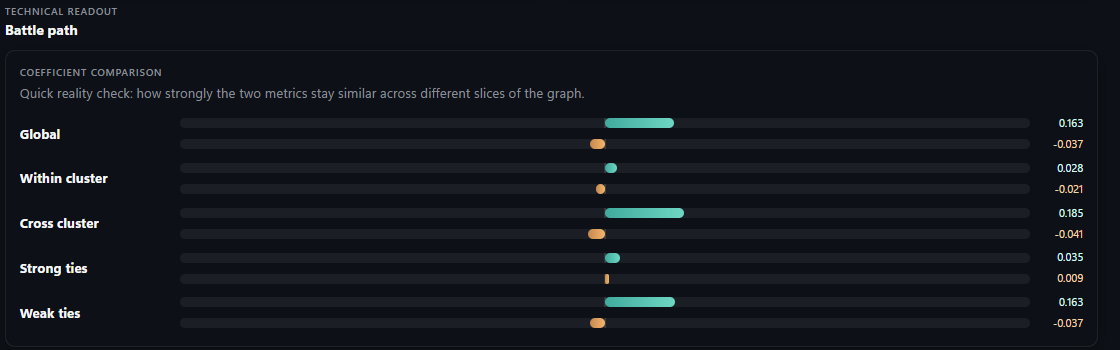
\includegraphics[width=0.98\textwidth,height=0.36\textheight,keepaspectratio]{sq-assortavity-battlepath-readout.png}
\caption{\texttt{soloq} battle-path technikai readout. A képernyőn az \texttt{opscore} pozitív, de mérsékelt értékei látszanak, míg a \texttt{feedscore} globálisan, within-cluster és cross-cluster bontásban is negatív közeli értékeket vesz fel.}
\end{figure}

\begin{figure}[H]
\centering
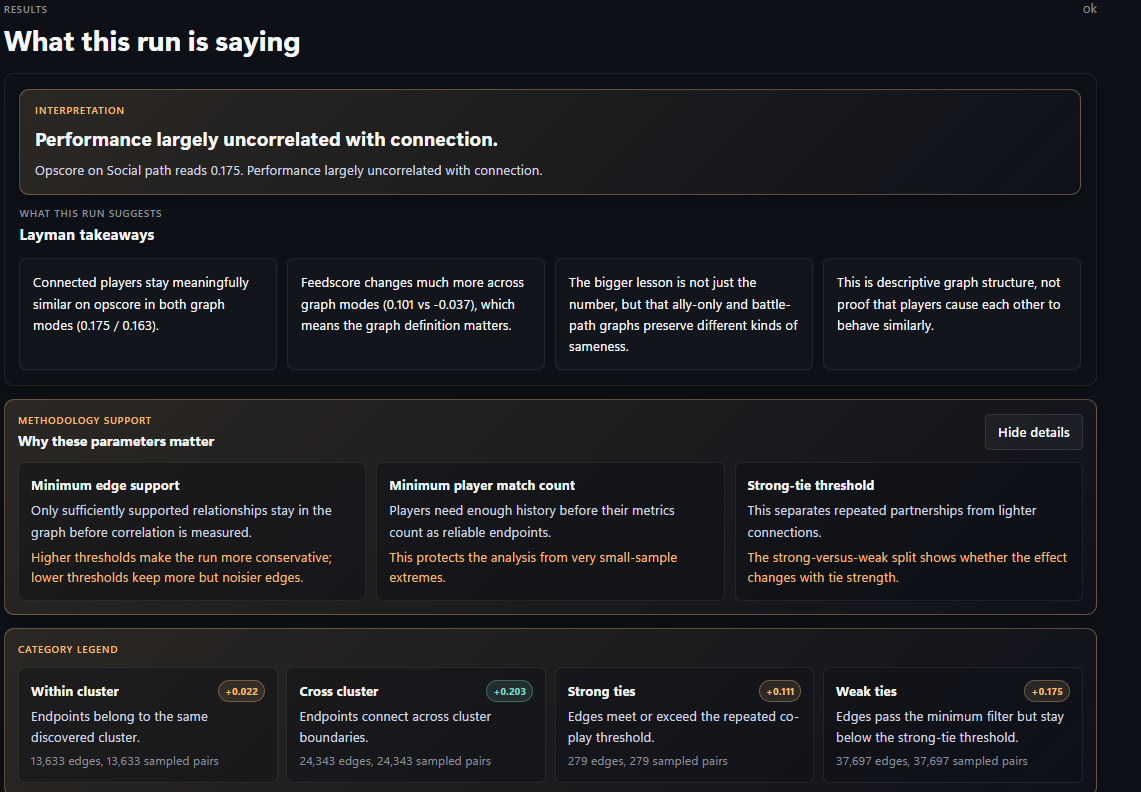
\includegraphics[width=0.98\textwidth,height=0.58\textheight,keepaspectratio]{sq-assortavity-layman-takeaways.png}
\caption{\texttt{soloq} közérthető frontend-összegzés. A képernyő azt foglalja össze, hogy az \texttt{opscore} hasonlóság mindkét gráfmódban megmarad, de a \texttt{feedscore} jelentősen változik; a módszertani panel külön jelzi, hogy a minimum support, a minimum meccsszám és az erős kapcsolat küszöbe befolyásolja, mennyire konzervatív a futtatás.}
\end{figure}

A \texttt{soloq} dataset kontrollszerepe itt látszik igazán. A pozitív \texttt{opscore} asszortativitás nem tűnik el, tehát a teljesítményhasonlósági jel nem kizárólag Flex Queue sajátosság. Ugyanakkor a social-path érték alacsonyabb, a strong-tie minták kicsik, és a \texttt{feedscore} battle-path módban negatív közeli eredményt ad. Ez azt támasztja alá, hogy a SoloQ inkább egyéni teljesítmény- és matchmaking-rekurrencia kontrollként értelmezhető, nem pedig stabil premade-kapcsolati hálóként.

\section{Mit mondanak ezek a számok?}

Mindkét datasetben egyértelműen pozitív asszortativitás jelenik meg az \texttt{opscore} mentén a \texttt{social-path} módban. Ez azt jelzi, hogy a szövetségesi kapcsolatokra épülő gráfban az összekapcsolt játékosok teljesítményprofilja nem véletlenszerűen keveredik.

A \texttt{feedscore} viselkedése jóval érzékenyebb a gráfmódra. A \texttt{social-path} módban mindkét dataseten mérsékelt pozitív jel látható, de a \texttt{battle-path} módban szinte nullára esik (flexset: $-0.0108$, soloq: $-0.0366$), a soloq esetén negatívba fordul. Ez azt mutatja, hogy az ellenfélkapcsolatok bevonásával a halálokon alapuló hibamutató elveszíti a társas-kapcsolati hasonlósági szerkezetet.

A két dataset közötti különbség: a flexset \texttt{social-path opscore} asszortativitása (0.2346) magasabb, mint a soloq-é (0.1750). Ez összhangban van azzal az értelmezési kerettel, hogy a Flex Queue erősebb visszatérő csapattársi szignált hoz létre, és ezért a gráf jobban tükrözi a hasonló teljesítményű játékosok összecsoportosulását.

Fontos különbség az is, hogy a battle-path mód mindkét datasetben lényegesen több élt vizsgál, de ez nem feltétlenül erősíti a korrelációt. A \texttt{flexset} esetén az élminta 61\,938-ról 179\,492-re nő, mégis csökken az \texttt{opscore} asszortativitás, és eltűnik a \texttt{feedscore} jel. A \texttt{soloq} esetén ugyanez a minta 37\,976-ról 84\,393-ra bővül, miközben a \texttt{feedscore} negatív közeli értéket vesz fel. Ez módszertanilag fontos: több él nem automatikusan jobb bizonyíték, ha az élhalmaz szemantikája kevertebb.

\subsection{Az \texttt{opscore} robusztusabb mint a \texttt{feedscore}}

Az \texttt{opscore} asszortativitása minden vizsgált módban pozitív marad. Ez az összetett, nyolc artifaktból súlyozott kompozit mutató erőssége: szemben a \texttt{feedscore} egyszerűbb halálközpontú képletével, az \texttt{opscore} több dimenzióból integrálja a teljesítményt, és ezért gráfprojekció-robusztusabb jelet ad. Nem azt állítjuk, hogy az \texttt{opscore} ``objektív igazság'' - a súlyok kézi tervezésűek és nem statisztikailag kalibráltak - de empirikusan megmutatja, hogy a gráf és a score-réteg között érdemi kapcsolat van, és ez a kapcsolat nem tűnik el gráfmódváltáskor.

\subsection{Gráfmód-érzékenység mint módszertani eredmény}

Ha mindkét metrika minden gráfmódban azonos értéket adna, akkor a gráfdefiníció nem hordozna önálló tartalmat. A jelen esetben az \texttt{opscore} csökkenése (flexset: 0.2346 → 0.1461, soloq: 0.1750 → 0.1625) a \texttt{battle-path} módban és a \texttt{feedscore} nullára esése azt mutatja, hogy a kapcsolatok szemantikája valóban meghatározza a teljesítményhasonlóság mérhetőségét. Ez megerősíti, hogy a projekt két gráfmódjának megkülönböztetése empirikusan indokolt módszertani döntés.

\subsection{Következtetés}

Az asszortativitási fejezet fő következtetése az, hogy a teljesítményhasonlóság mérhető, de nem univerzális tulajdonsága a játékosgráfnak. A legerősebb és legjobban értelmezhető jel a \texttt{flexset} social-path \texttt{opscore} futtatásában jelenik meg. Ez támogatja azt az állítást, hogy a Flex Queue szövetségesi hálózata alkalmas asszociatív játékosgráfként való elemzésre.

Ezzel szemben a \texttt{feedscore} eredmények azt mutatják, hogy az egyszerűbb, halálközpontú teljesítménymutató kevésbé stabil gráfanalitikai attribútum. Social-path módban még hordoz pozitív jelet, battle-path módban azonban a kapcsolat közel semlegessé vagy enyhén negatívvá válik. A dolgozat ezért az \texttt{opscore}-t kezeli robusztusabb teljesítményprofilként, miközben nyíltan rögzíti, hogy ez kézi súlyozású kompozit mutató, nem végleges statisztikai kalibráció.

A Flex--SoloQ összehasonlítás szintén a fejezet módszertani eredménye. A SoloQ pozitív, de gyengébb \texttt{opscore} jele arra utal, hogy a magasabb teljesítményű játékosok matchmaking-környezetében is keletkezik hasonlósági szerkezet. A Flex Queue erősebb social-path eredménye viszont azt jelzi, hogy a visszatérő csapattársi kapcsolatok külön, jobban interpretálható asszociatív réteget képeznek. Ebből nem következik, hogy a játékosok okozzák egymás teljesítményét; a helyes állítás az, hogy az adott gráfprojekcióban az összekapcsolt játékosok mérhetően hasonlóbb teljesítményprofilokat mutatnak.

\section{A randomizációs infrastruktúra helye}

A kódbázisban az asszortativitáshoz randomizációs szignifikanciateszt is tartozik. Ez fontos fejlesztési irány, mert a leíró korrelációt nullmodellel is érdemes összevetni. A jelen dolgozatban azonban a fő eredményeket a közvetlenül ellenőrzött leíró és bontott futtatásokra alapozom. Így a szöveg őszinte marad: a szignifikanciakeret jelen van a rendszerben, de a hangsúly még nem a teljes permutációs kísérletsorozaton van.

% ===== chapters/17-parhuzamos-brandes-fele-betweenness-centralitas.tex =====
\chapter{Párhuzamos Brandes-féle betweenness centralitás}

\section{Miért szükséges a betweenness centralitás ebben a kontextusban?}

A bridge-orbit vizualizáció már a Graph V2 pipeline-ból is meghatároz egyes csomópontokat és klasztereket „hidaknak" az \texttt{orbitScore} és \texttt{orbitRadius} mezők alapján. Ezek a mezők azonban vizuális heurisztikák: a kereszt-klaszter szövetségesi támasz, az összekötött klasztercsoport-szám és a tagszám kombinációján alapulnak, de nem ellenőrzik, hogy a jelölt csomópontok valóban a legtöbb legrövidebb útvonal metszéspontján helyezkednek-e el. Az igazi Brandes-féle közöttiség centralitás (betweenness centrality) éppen ezt az ellenőrzést teszi lehetővé: megméri, hogy egy csomópont hány legrövidebb út mentén helyezkedik el a gráfban, és ezért nem becslésen, hanem teljes gráfbejáráson alapul.

A projektben a betweenness centralitás a \texttt{backend/pathfinder-rust/src/engine/centrality.rs} modulban van implementálva. Az implementáció több fontos döntést tartalmaz, amelyek mindegyike önálló módszertani állítás.

\begin{figure}[h]
\centering
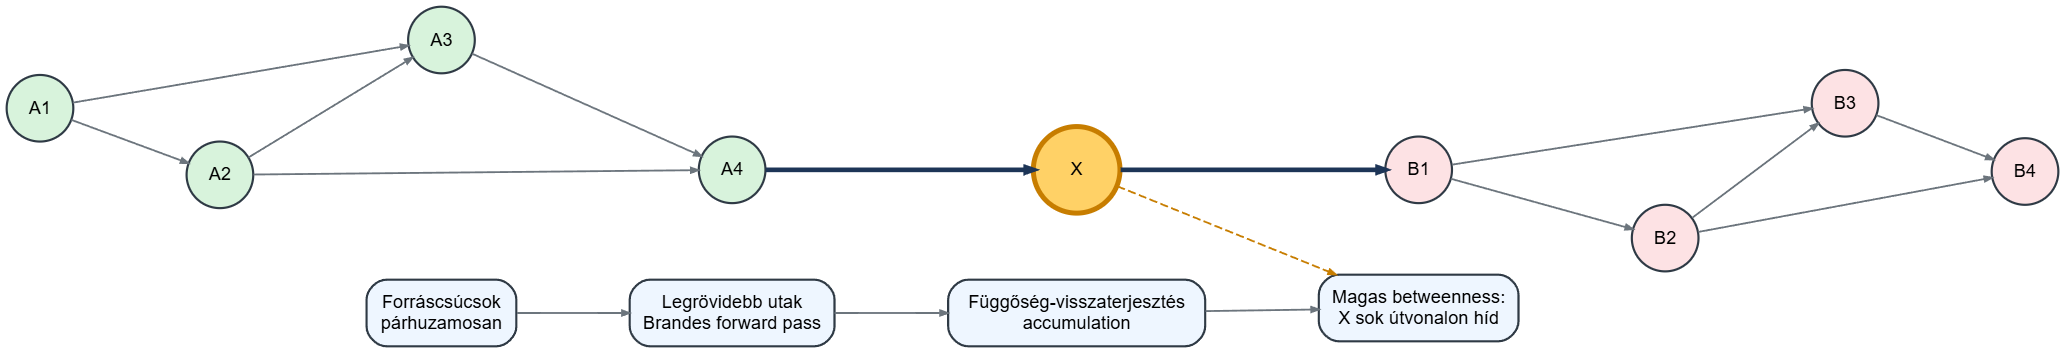
\includegraphics[width=0.92\textwidth]{assets/diagrams/thesis_brandes_bridge_graphviz.png}
\caption{A betweenness centralitás intuitív értelmezése: a hídcsomópont sok klaszterközi legrövidebb útvonalon jelenik meg, ezért magas Brandes-pontszámot kap.}
\label{fig:brandes-bridge-graphviz}
\end{figure}

\section{Az algoritmus: Brandes 2001}

A Brandes-algoritmus \cite{brandes2001} a hagyományos $O(n^3)$ komplexitású betweenness-számítást $O(nm)$-re csökkenti (irányítatlan gráfra, ahol $n$ a csomópontok és $m$ az élek száma). Az ötlet az, hogy a csomópontonkénti legrövidebb-út fákat nem kell külön-külön tárolni: a forráscsomópontból induló BFS/Dijkstra-futtatás eredményéből egy visszaterjesztési lépésben kiszámítható az összes közötti wt-részleges járulék.

A Brandes-algoritmus lépései forráscsomópontonként:

\begin{enumerate}
    \item Dijkstra/BFS futtatás a forrásból: kiszámolja a $\sigma[s][v]$ értéket (legrövidebb utak száma $s$-től $v$-ig) és az $dist[s][v]$ távolságokat.
    \item A feltehetős csomópontok fordított sorrendben kerülnek feldolgozásra (a stack-ból): minden $w$-re, amelynek előde $v$ a legrövidebb úton, a $\delta[s][v]$ függőségi mutató a következőképpen frissül:
    \begin{equation}
    \delta[s][v] \mathrel{+}= \frac{\sigma[s][v]}{\sigma[s][w]} \cdot (1 + \delta[s][w])
    \end{equation}
    \item A forrást kivéve minden csomóponthoz hozzáadódik a $\delta[s][v]$ érték a globális betweenness-számlálóhoz.
\end{enumerate}

Irányítatlan gráfra az összes forrás feldolgozása után az eredmény felezése szükséges, mert minden $(s, t)$ és $(t, s)$ pár kétszer volt megszámlálva. A normalizálás az $(n-1)(n-2)/2$ maximális útvonalszámra vetít. Az implementáció pontosan ezt a logikát követi a \texttt{source\_dependencies()} és a \texttt{finalize\_undirected\_scores()} függvényekben.

\section{A súlyozott mód és a költségmodell}

A centralitás-modulban a súlyozott módban az él költsége az \texttt{edge\_cost()} függvény alapján:

\begin{equation}
c(u,v) = \left\lceil \frac{10^6}{\max(1, w(u,v))} \right\rceil
\end{equation}

ahol $w(u,v)$ az adott gráfmódnak megfelelő kapcsolaterősség (\texttt{allyWeight} social-path módban, \texttt{total\_matches} battle-path módban). Az \texttt{1\_000\_000}-os skálázási konstans (\texttt{COST\_SCALE}) integeraritmetikai pontosságot biztosít: az egészre kerekített reciprok kis élsúlyoknál nagy, erős kapcsolatoknál kis költséget ad, és az egész aritmetika determinisztikus rendezési viselkedést biztosít a prioritásos sorban.

Súlyozatlan módban az összes él ára \texttt{COST\_SCALE} = $10^6$, ami egyenértékű az eredeti, súlyozatlan Brandes-bejárással.

Ez a kettős mód (súlyozott/súlyozatlan) közvetlenül összemérhető a Pathfinder-modulban alkalmazott \texttt{traversal\_cost()} képlettel, ahol a skálázási konstans 1000. A centralitás-modul pontosabb integer-aritmetikát használ a nagyobb összegek miatt.

\section{Párhuzamos végrehajtás Rayonnal}

A Rust \texttt{rayon} könyvtára automatikus munkalopásos (work-stealing) párhuzamosságot tesz lehetővé. A centralitás-modul ezt a következő stratégiával alkalmazza:

\begin{enumerate}
    \item A forráscsomópontok halmazát $k$ egyenlő méretű csomóponthalmazra osztja, ahol $k = \min(n, 4 \cdot \text{szálak száma})$.
    \item Minden halmazt egy párhuzamos rayon-feladatban dolgoz fel: a lokális $\delta$ vektor független a többi résztől.
    \item Az összegzés után a részeredmény-vektorok deterministikusan összeadódnak.
    \item A párhuzamos eredményt a soros eredménnyel összevethető maximális abszolút eltérés (\texttt{max\_abs\_delta}) jellemzi.
\end{enumerate}

A determinizmus biztosítása kulcsfontosságú: a forráscsomópontok rendezése és a chunk-határok rögzítése garantálja, hogy azonos input esetén mindig ugyanaz a kimenet. A tesztcsomag (\texttt{parallel\_matches\_serial}) ezt explicit módon ellenőrzi.

\begin{figure}[H]
\centering
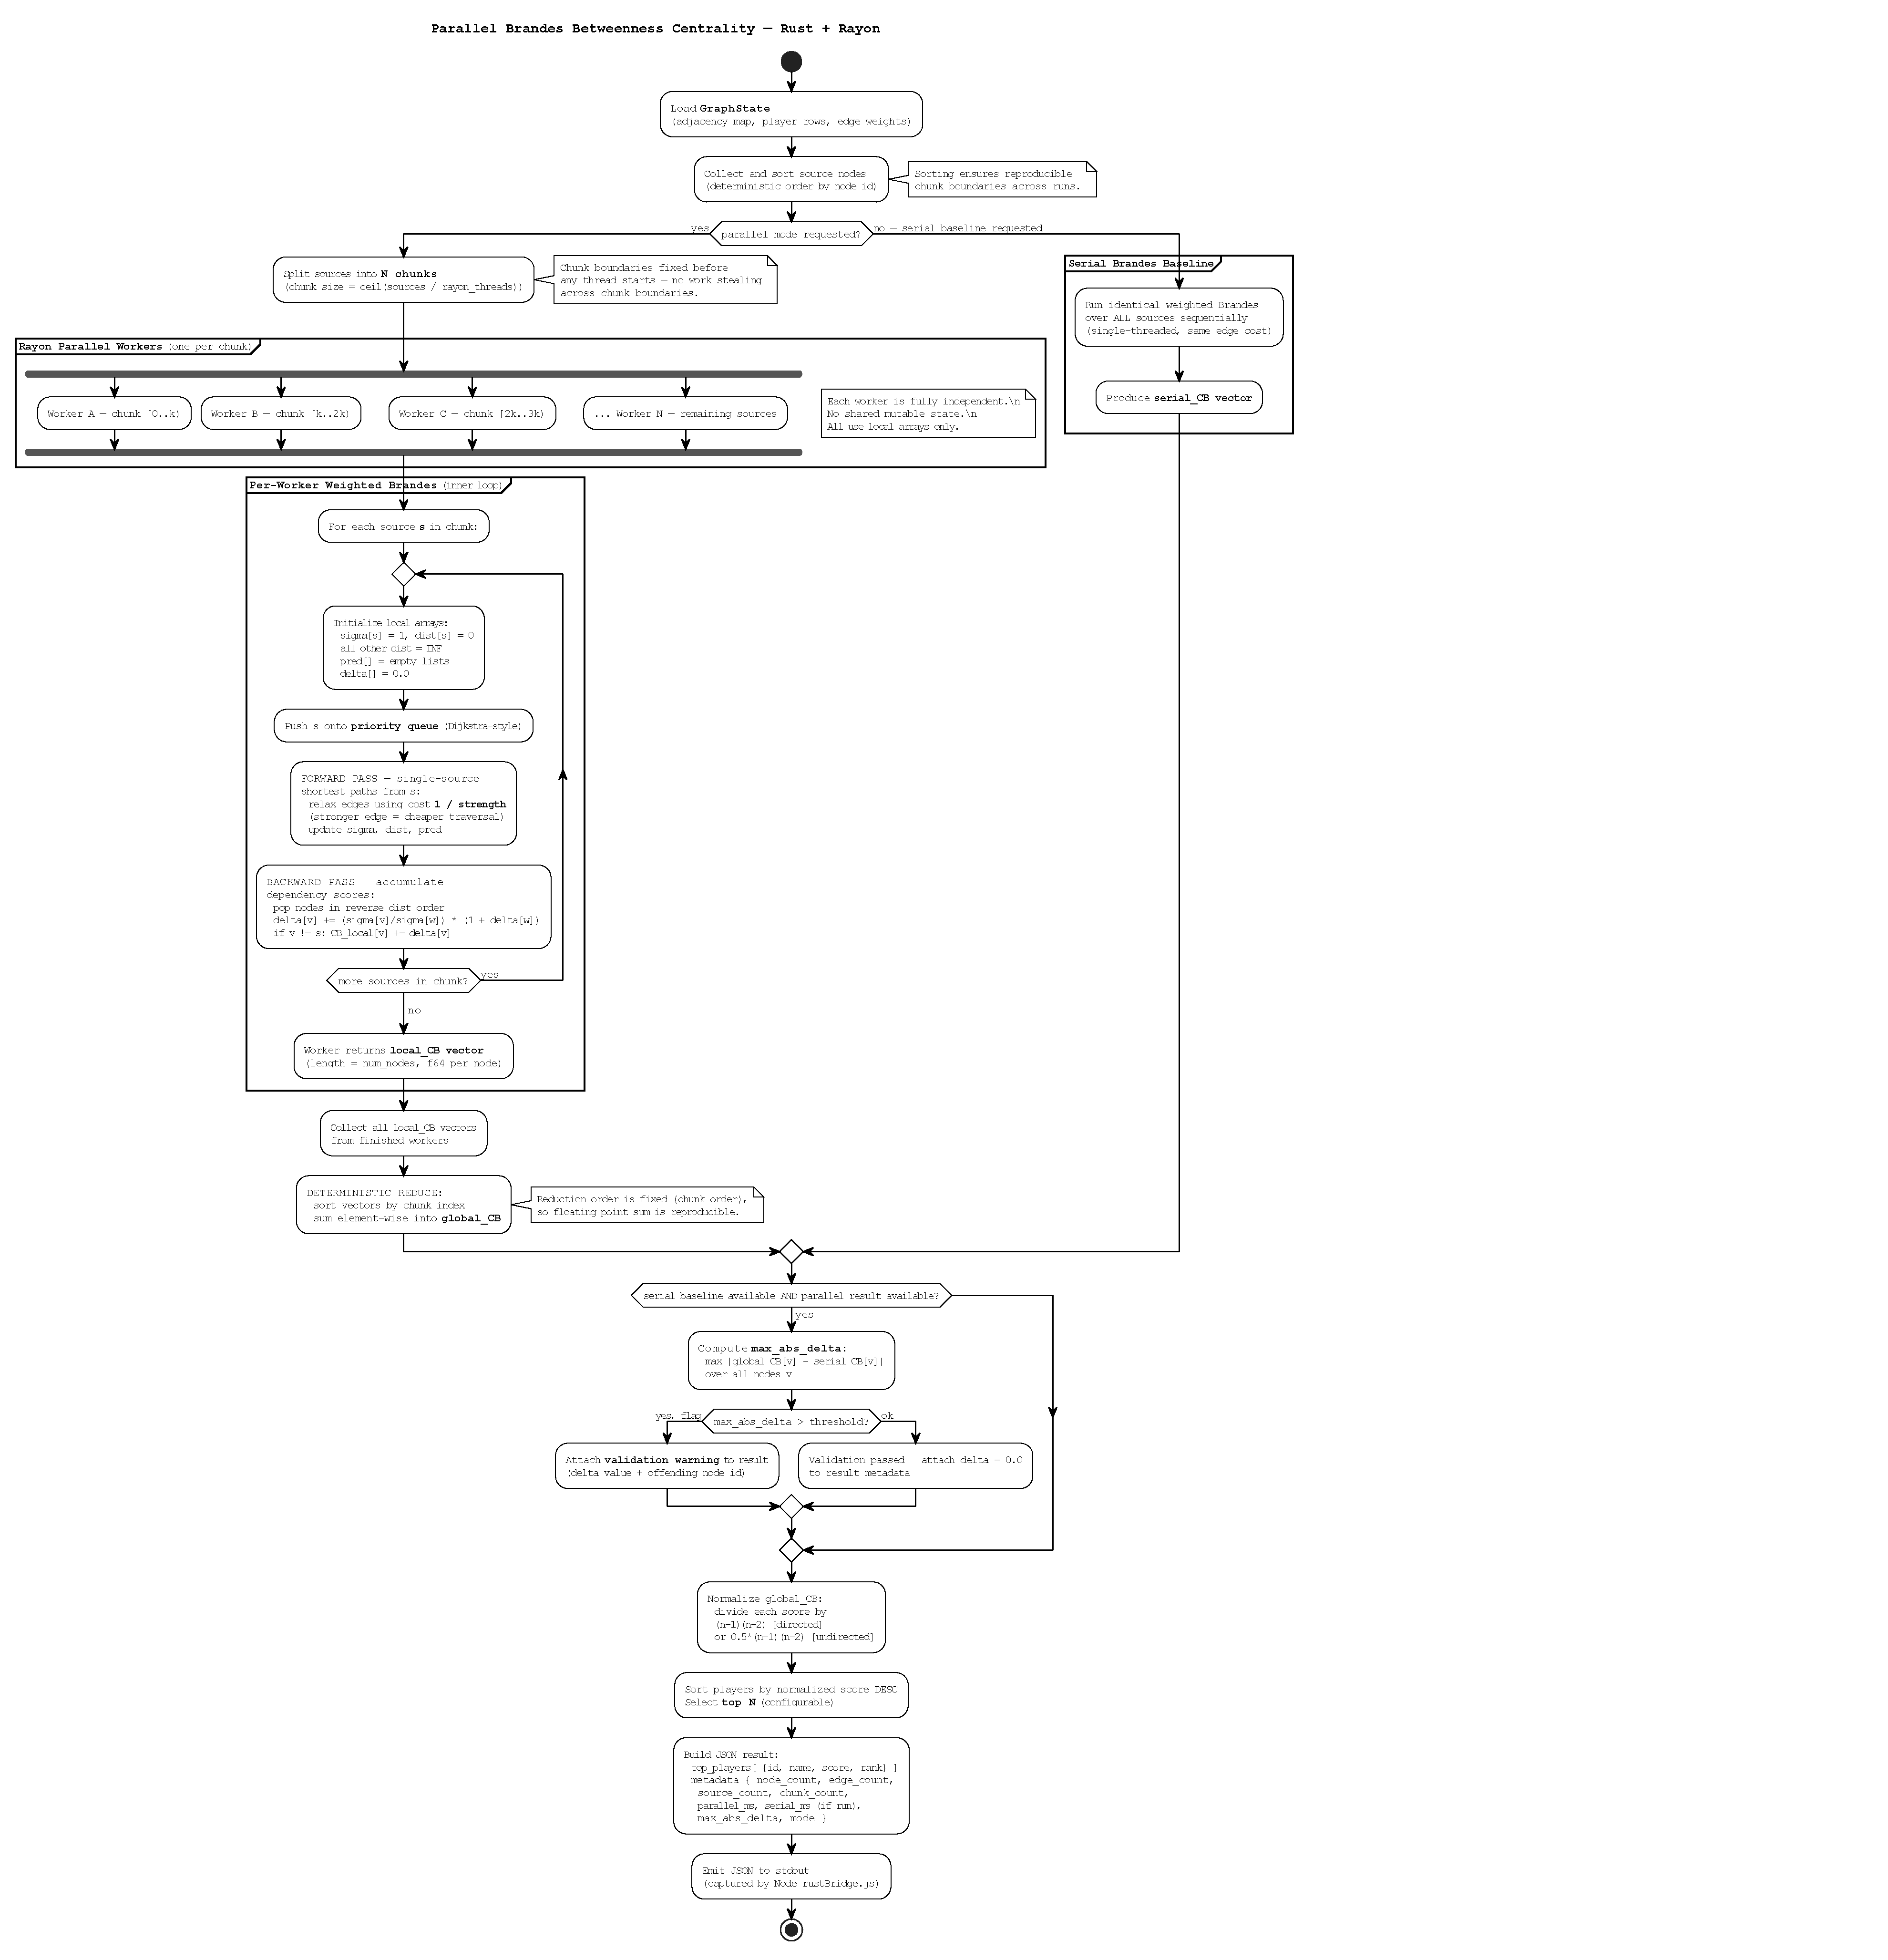
\includegraphics[width=0.98\textwidth,height=0.76\textheight,keepaspectratio]{parallel brandes activity diagram.pdf}
\caption{A párhuzamos Brandes-futtatás aktivitásdiagramja a \texttt{parallel-brandes.puml} forrás alapján. A folyamat a \texttt{GraphState} betöltésével és a forráscsomópontok determinisztikus rendezésével indul, majd párhuzamos módban fix chunkokra bontja a forrásokat. Minden Rayon worker saját lokális tömbökkel futtat súlyozott Brandes-bejárást, \texttt{1/strength} élköltséggel; a lokális centralitásvektorok chunk-sorrendben, determinisztikusan redukálódnak globális eredménnyé. Ha soros baseline is készül, a rendszer \texttt{max\_abs\_delta} értékkel ellenőrzi a párhuzamos és soros kimenet egyezését, majd normalizál, rangsorol és JSON választ ad vissza a Node.js hídnak.}
\end{figure}

\begin{figure}[H]
\centering
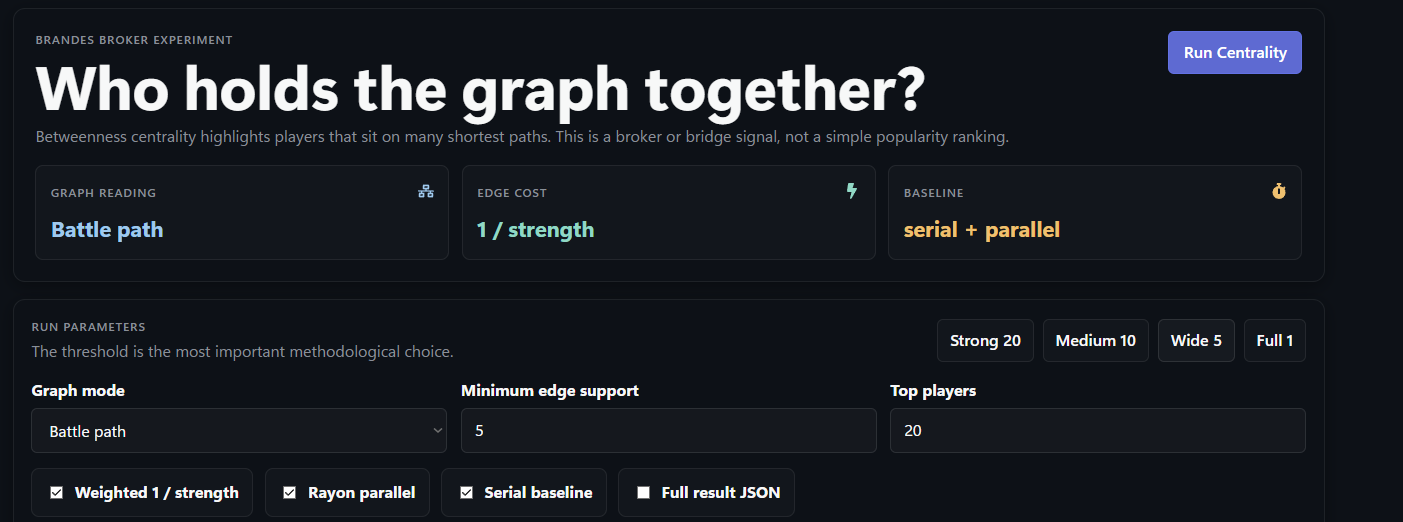
\includegraphics[width=0.98\textwidth,height=0.52\textheight,keepaspectratio]{brandes-config.png}
\caption{A Brandes betweenness centralitás frontend konfigurációs felülete. A képen a \texttt{battle-path} gráfolvasat, az \texttt{1/strength} élköltség, a soros és párhuzamos baseline összehasonlítás, az 5-ös minimum éltámogatás, a top 20 játékos kérése, valamint a súlyozott, Rayon-párhuzamos és soros baseline opciók láthatók.}
\end{figure}

\begin{table}[H]
\centering
\caption{A betweenness centralitás-modul főbb konfigurációs dimenzióinak összefoglalója}
\begin{tabular}{lll}
\toprule
\textbf{Dimenzió} & \textbf{Lehetséges értékek} & \textbf{Hatás} \\
\midrule
Gráfmód & social-path, battle-path & Melyik élhalmazon fut \\
Súlyozás & igen / nem & \texttt{edge\_cost()} visszaadott értéke \\
Párhuzamos & igen / nem & rayon vs. soros Brandes \\
Soros baseline & igen / nem & Delta-ellenőrzés a kimenetben \\
Min. élsúly & $\geq 1$ & Gyenge élek kizárása \\
\bottomrule
\end{tabular}
\end{table}

\section{A projection felépítése}

A \texttt{build\_projection()} függvény a \texttt{GraphState} pair\_relations térképéből iterál. Az élek sorrend szerint rendezve kerülnek feldolgozásra, így a projekció determinisztikus. Kizárt élek:

\begin{itemize}
    \item nulla \texttt{support} értékűek az adott gráfmódban;
    \item minimum élsúly alatt lévők (\texttt{skipped\_low\_support\_edges});
    \item rossz formátumú kulcsok (\texttt{skipped\_invalid\_edges}).
\end{itemize}

A csomópontok $\alpha$-betű sorrendben indexelődnek (\texttt{BTreeSet}), és a szomszédsági lista minden csúcsnál szintén rendezett. Ez garantálja a determinizmust akkor is, ha a \texttt{HashMap}-ben tárolt pair\_relations bejárási sorrendje változó.

\section{Normalizálás és eredményinterpretálás}

A normalizált betweenness érték egy $[0, 1]$ intervallumba esik, ahol az 1.0 értékű csomópont minden lehetséges $s \to t$ legrövidebb úton rajta van. A maximálisan normalizált érték ritka: csak csillag-topológia centerének normalizált betweenness értéke pontosan 1.0.

Az egységtesztek ezt a három alapesetet explicit ellenőrzik:

\begin{enumerate}
    \item \textbf{Lánc-topológia} (path graph): a belső csomópontok magasabb betweenness-t kapnak, mint a végpontok.
    \item \textbf{Csillag-topológia} (star graph): a center normalizált értéke pontosan 1.0.
    \item \textbf{Dumbbell-topológia}: a hidat képező csomópont rangsorolódik legelőre.
    \item \textbf{Súlyozási teszt}: erős parellelút esetén a súlyozatlan mód a közvetlen élt preferálja, a súlyozott mód az erősebb közvetett utat.
    \item \textbf{Soros-párhuzamos egyezés}: determinisztikus azonosság bizonyítva (\texttt{max\_abs\_delta == 0}).
\end{enumerate}

\begin{figure}[H]
\centering
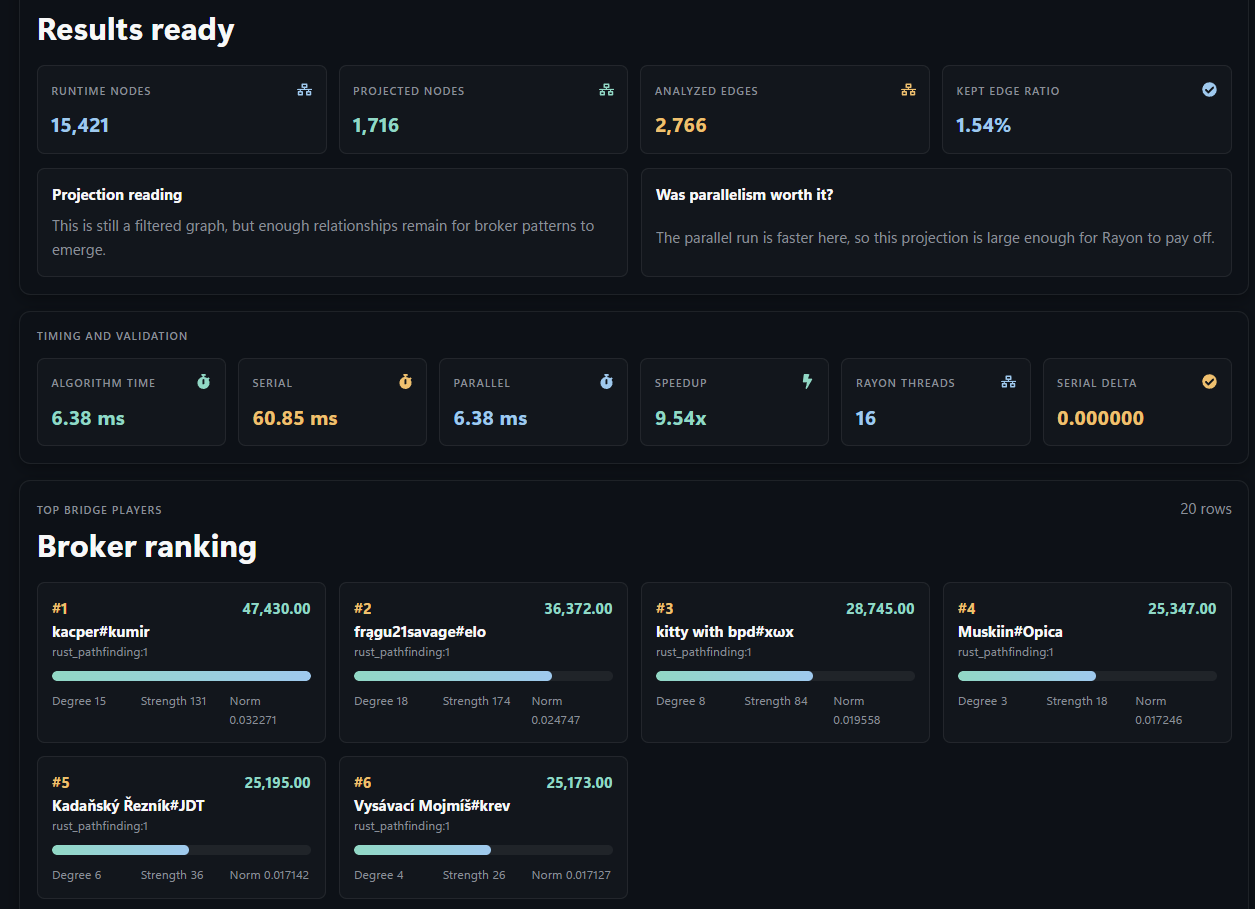
\includegraphics[width=0.98\textwidth,height=0.68\textheight,keepaspectratio]{brandes-result.png}
\caption{Brandes betweenness centralitás eredményképernyő. A futás 15\,421 runtime csomópontból 1\,716 projektált csomópontot és 2\,766 elemzett élt tartott meg, ami 1.54\%-os megtartott élhányadot jelent. A párhuzamos futás 6.38 ms alatt, a soros baseline 60.85 ms alatt futott, így a képernyő 9.54-szeres gyorsulást, 16 Rayon szálat és 0.000000 soros-párhuzamos deltát mutat; alul a top broker játékosok rangsora látható raw és normalizált centralitási értékekkel.}
\end{figure}

A képernyő alapján a kiválasztott, 5-ös minimum supporttal szűrt \texttt{battle-path} projekció már elég nagy ahhoz, hogy a Rayon-párhuzamosítás mérhetően hasznos legyen, miközben a \texttt{serial delta} nulla marad. Ez egyszerre fontos teljesítmény- és validációs jel: a párhuzamos futás nem csak gyorsabb, hanem a soros baseline-nal numerikusan egyező eredményt ad ezen a futtatáson.

\section{Centralitás a bridge-orbit hipotézis tesztelésére}

A bridge-orbit layout ($\S$\ref{sec:graph_v2_artifact}) az \texttt{orbitScore} és \texttt{orbitRadius} mezőkkel azonosítja a kiemelten összekötő klasztereket. Ezeket a heurisztikus pontszámokat egyelőre nem vetítettük össze Brandes-betweenness értékekkel, de a modul elkészültével ez a validálás elvégezhető.

A várható hipotézis: a legmagasabb \texttt{crossAllySupport} és \texttt{connectedAllyClusterCount} értékű klaszterek átlagos Brandes-betweenness értéke szignifikánsan magasabb az alacsony orbit-score-úakénál. Ha ez teljesül, az megerősíti, hogy az orbit-heurisztika jó előszűrője a valódi topológiai hidat képező csomópontoknak. Ha nem teljesül, az a heurisztika korlátaira világít rá és pontosítja a vizualizáció értelmezési keretét.

Ez a jövőbeli vizsgálat pontosan az a fajta módszertanilag indokolt bővítés, amelyről a \texttt{research-workflow} szemlélet szól: a meglévő adatból egy explicit, megcáfolható hipotézis tesztelhető, és az eredmény akár megerősíti, akár megcáfolja a korábbi vizuális heurisztikát.

\begin{figure}[H]
\centering
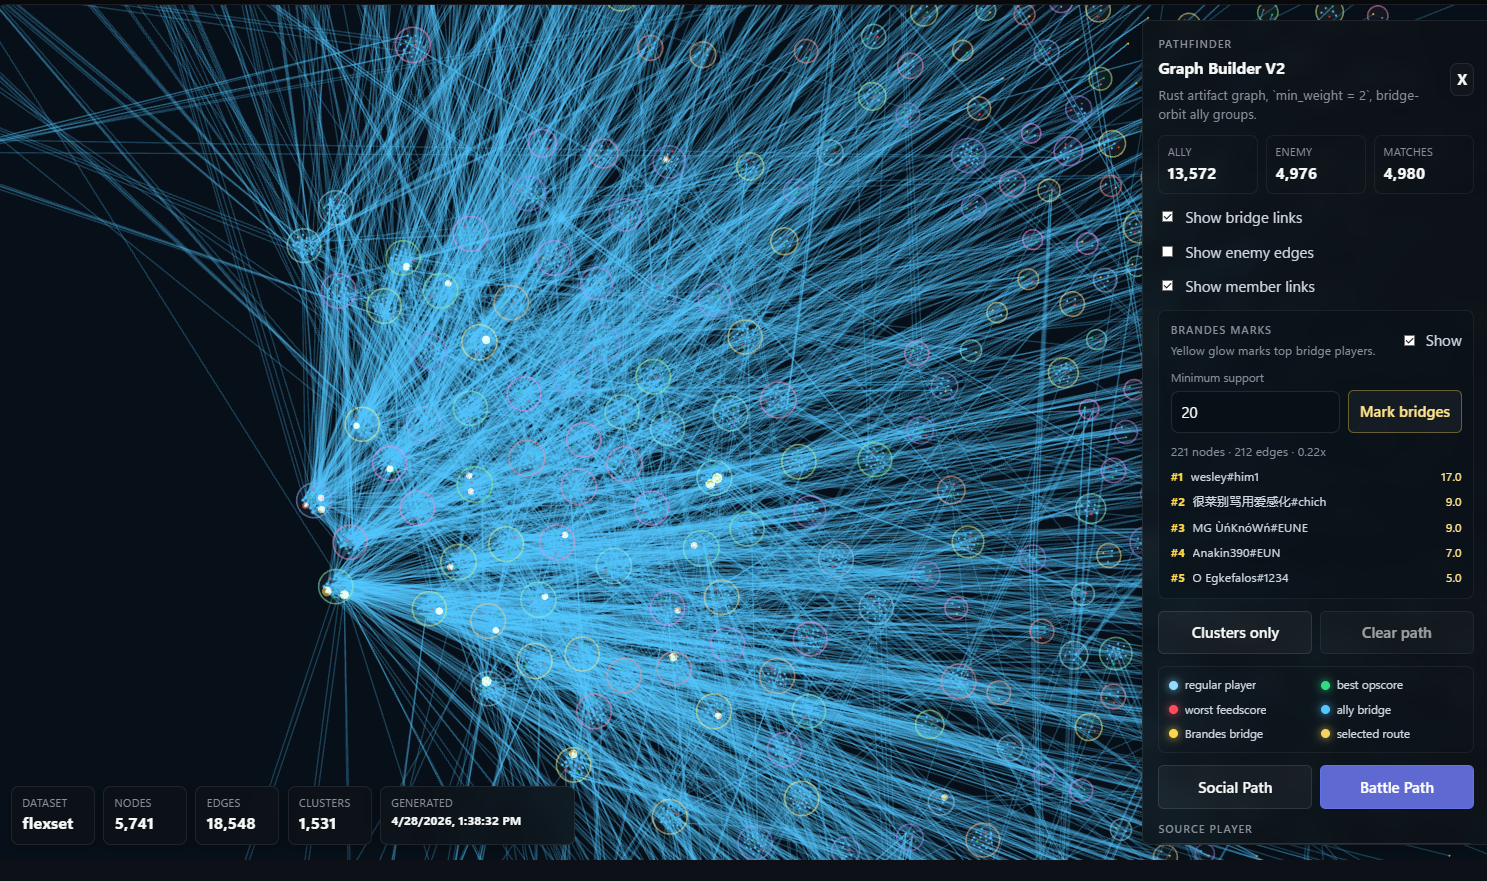
\includegraphics[width=\textwidth,height=0.78\textheight,keepaspectratio]{graph-brandes-brokerinyellow.png}
\caption{A betweenness centralitás alapján azonosított broker játékosok a gráfban, sárgával kiemelve. A kiemelés azokat a csomópontokat jelöli, amelyek a Brandes-algoritmus szerinti normalizált \texttt{betweenness} értéke a legmagasabb — vagyis ezek a csomópontok helyezkednek el a legtöbb legrövidebb út mentén. Ezek a bridge-jelöltek az \texttt{orbitScore}-alapú vizuális heurisztika és a tényleges topológiai centralitás összevetésének szemléletes kiindulópontja.}
\end{figure}

\section{Kísérletfuttató infrastruktúra és nullmodellek}

A Rust motor nem csak egyedi analitikai kéréseket tud kiszolgálni, hanem strukturált kísérleteket is tud futtatni a \texttt{backend/pathfinder-rust/src/engine/experiments.rs} modulon keresztül.

\subsection{Signed-balance sweep mint módszertani diagnosztika}

A \texttt{SignedBalanceSweepRequest} egy kötegelt futási kérés, amely egyszerre több minimum-élsúly és döntetlen-kezelési politika kombinációt futtat le, és az összes eredményt egységes \texttt{SignedBalanceSweepResponse} válaszban adja vissza. A sweep sémaverziója (\texttt{signed-balance-sweep-v1}) az eredmények jövőbeli összehasonlíthatóságát biztosítja.

Minden egyes sweep-futás az alapfuttatással azonos Rust kódon megy keresztül, így az összes kombinált eredmény egységes implementációs alapra támaszkodik. A sweep főbb paraméterei:

\begin{itemize}
    \item \texttt{min\_support\_values}: vizsgált minimális élsúlyok listája;
    \item \texttt{tie\_policies}: vizsgált döntetlen-kezelési politikák listája (\texttt{exclude}, \texttt{ally}, \texttt{enemy});
    \item \texttt{graph\_modes}: \texttt{social-path} és/vagy \texttt{battle-path}.
\end{itemize}

Ez lehetővé teszi, hogy egy kérésben teljes érzékenységi mátrix készüljön, például: minden min\_support × tie\_policy kombinációra megkapjuk az analizált triádok számát és az egyensúlyi arányt. A dolgozatban ezt már nem fő eredményként használom, hanem annak ellenőrzésére, hogy mennyire erősen függ a formális signed-balance kimenet a projekciós döntésektől. A sweep így a módszertani határ dokumentálására szolgál.

\subsection{Asszortativitási szignifikanciateszt}

Az \texttt{AssortativitySignificanceRequest} permutációs nullmodellt futtat: véletlenszerűen kever össze játékos--score párokat az éleken, és az így kapott nulldisztribúcióval veti össze a megfigyelt korrelációt. A determinisztikus RNG-mag (\texttt{SystemTime::UNIX\_EPOCH} alapú, de rögzíthető) garantálja a reprodukálhatóságot.

A nullmodell-futtatás főbb jellemzői:

\begin{itemize}
    \item permutáció-szám konfigurálható (\texttt{num\_permutations});
    \item a figyelt korreláció ($r_\mathrm{obs}$) összehasonlítható a null-eloszlás átlagával és szórásával;
    \item a $p$-érték az $r_\mathrm{null} \geq r_\mathrm{obs}$ arányból becsülhető;
    \item a sémaverziójú kimenet (\texttt{assortativity-significance-v1}) az eredményeket önmagukon belül értelmezhetővé teszi.
\end{itemize}

A jelen dolgozatban a szignifikanciafuttatások megléte a rendszerben dokumentált, de az összes kombinációra kiterjedő, végleges nullmodell-kísérletsorozat a jövőbeli fejlesztések közé tartozik. A hangsúly egyelőre az asszortativitás leíró korrelációin és a dataset-összehasonlításon van, amelyek önmagukban is érvényes empirikus eredmények.

\subsection{A kísérletfuttató infrastruktúra módszertani értéke}

A sweep és a szignifikanciateszt léte nem csak technikai kényelmi funkció. Módszertanilag azt jelenti, hogy a dolgozatban közölt eredmények reprodukálhatók és bővíthetők: ugyanazon infrastruktúrán egy jövőbeli vizsgálat egyre finomabb paraméterekkel futhat le, anélkül hogy az alapimplementációt módosítani kellene. Ez összhangban van a reprodukálható kutatás alapelvével \cite{sandve2013}: a szoftver, nem csak a szöveg hordozza a módszertani döntéseket.

% ===== chapters/18-kiserleti-futtatasok-validacio-es-eredmenyek.tex =====
\chapter{Kísérleti futtatások, validáció és eredmények}

\section{Verifikációs lépések}

A dolgozat elkészítésekor a rendszer aktuális állapotát nemcsak a dokumentáció, hanem közvetlen futtatás alapján is ellenőriztem. A főbb helyi ellenőrzések:

\begin{itemize}
    \item a Rust futtatókörnyezet sikeresen lefuttatta az \texttt{assortativity} parancsot;
    \item a Rust futtatókörnyezetben a \texttt{signed-balance} parancs kísérleti modulként továbbra is futtatható volt;
    \item a fő adatbázis és dataset-nyilvántartás elérhető és olvasható volt;
    \item a dolgozati frontend útvonalak közül az asszortativitási és központisági oldalak maradtak a fő analitikai folyamat részei.
\end{itemize}

Ez azért lényeges, mert a dolgozat ezen a ponton már nem csak tervekről, hanem ténylegesen végrehajtható modulokról számol be.

A verifikációs lépések tudatosan nem teljes funkcionalitástesztek voltak, hanem tézisszintű ellenőrzések. A cél itt az volt, hogy minden olyan rétegről legyen közvetlen bizonyíték, amelyre a dolgozat állításokat épít: a dataset-regiszter olvashatósága, a Rust analitikai parancsok futtathatósága, valamint a frontendoldalak fizikai jelenléte. Ez összhangban van a reprodukálható kutatási gyakorlat logikájával is: a szöveg és az alátámasztó futások között legyen világos kapcsolat \cite{sandve2013}.

\section{Az aktív állapot összefoglalása}

A 2026. április 28-án ellenőrzött aktív állapotban a rendszer az \texttt{soloq} datasetre épül, a \texttt{flexset} dataset a fő kutatási korpusz. Az adatkészletek és a gráfállapot összefoglalása:

\begin{table}[H]
\centering
\caption{A jelenlegi rendszerállapot fő mennyiségi mutatói - \texttt{flexset} és \texttt{soloq}}
\begin{tabular}{lrr}
\toprule
\textbf{Mutató} & \textbf{flexset} & \textbf{soloq} \\
\midrule
Meccs-JSON állományok & 4981 & 2001 \\
Graph V2 meccsszám & 4980 & 2000 \\
Nyers játékosok (\texttt{players.db}) & 15\,147 & 2822 \\
Finomított játékosok (\texttt{playersrefined.db}) & 15\,421 & 6768 \\
Klaszterek (\texttt{playersrefined.db}) & 599 & 140 \\
Klasztertagok & 5741 & 1538 \\
Látható Graph V2 csúcsok & 5741 & 1538 \\
Látható Graph V2 élek & 18\,548 & 4111 \\
Átlagos élsúly (Graph V2) & 3.405 & 2.364 \\
Graph V2 klaszterek & 1531 & 870 \\
Átlagos klaszterméret & 3.750 & 1.768 \\
\bottomrule
\end{tabular}
\end{table}

Ezeket a számokat lépcsőzetesen kell olvasni. A finomított játékosszám a teljes score-réteg kiterjedése. A Graph V2 látható csúcsok száma már csak az érvényes klasztertagsággal rendelkező játékosokat tartalmazza. Minden réteg a saját, a megelőzőből leszűkített univerzumán számol, ezért a gráf- és score-alapú eredményeknél mindig ki kell mondani, hogy pontosan melyik populáción készültek.

A két dataset összehasonlítása megerősíti, hogy a \texttt{flexset} és a \texttt{soloq} lényegesen eltérő karakterű korpuszok, és ez az eltérés minden analitikai szinten mérhető.

\section{A korpusz összetétele mint értelmezési háttér}

Az eredmények értékeléséhez fontos hozzárakni, hogy a vizsgált korpusz nem homogén. A queue-eloszlás alapján a ranked módok dominálnak, de a rendszerben ARAM és normál meccsek is jelen vannak. Ez két következménnyel jár:

\begin{itemize}
    \item a gráf egy része erősen kompetitív, ismétlődő társas térből származik;
    \item egy másik része lazább, zajosabb kapcsolatokkal terhelt.
\end{itemize}

Éppen ezért a küszöbölés, az erős és gyenge kapcsolatok bontása, valamint a \texttt{social-path} és \texttt{battle-path} megkülönböztetése nem puszta technikai részlet, hanem az adatkorpuszból fakadó szükségszerűség.

Ez a felismerés a teljes eredményfejezetet meghatározza. Ha a korpusz heterogén, akkor a gráfmodellt sem lehet úgy kezelni, mintha egyetlen társas mechanizmust mérne. A \texttt{social-path} és \texttt{battle-path} különválasztása nem csupán algoritmus-beállítás, hanem módszertani védekezés a túlzó interpretáció ellen.

\section{A két klasztercsalád gyakorlati különbsége}

A perzisztált klasztereknél az is ellenőrizhető volt, hogy a Python és a Rust család eltérő karakterű. A \texttt{python\_population} klaszterek kicsit kisebb maximális méretűek és inkább populációs közösségképet adnak, míg a \texttt{rust\_pathfinding} klaszterek futásidejű szempontokhoz igazodnak, és jóval nagyobb maximumklasztert is tartalmaznak.

Ez összhangban van a rendszertervvel. A két klasztercsalád nem egymás hibás duplikátuma, hanem eltérő feladatokra optimalizált nézet.

\section{Analitikai eredmények}

Az asszortativitási eredmények részletes táblái és módszertani kifejtése a dedikált fejezetben kapott helyet. A strukturális egyensúly külön fejezetben csak módszertani határesetként szerepel: a formális implementáció megvan, de az enemy-élek szemantikája miatt nem használom fő empirikus eredményként. A két dataset összesített, szintetikus összehasonlítása a rákövetkező összehasonlító fejezetben található.

\section{A frontend és a rendszerkoherencia értékelése}

A projekt egyik fontos eredménye nem kizárólag a számszerű analitikában áll, hanem abban is, hogy a rendszer ma már koherens egészként működik. A jelenlegi állapotban:

\begin{itemize}
    \item az adatgyűjtés és dataset-kezelés külön rétegben történik;
    \item a pontszámítás explicit, ellenőrizhető képletekre épül;
    \item a gráfépítés és klaszterezés nem ad hoc frontend-logika;
    \item a futásidejű Rust réteg a gráfanalitikát külön kezeli;
    \item a frontend több specializált felületen, eltérő célok mentén mutatja meg az eredményeket.
\end{itemize}

Ez azért fontos, mert a dolgozat nem egyszerűen egy algoritmus vagy egy látványos oldal bemutatása, hanem annak dokumentálása, hogy ezek a részek együtt már egy kutatásképes rendszerként viselkednek.

A koherencia egyik kézzelfogható jele, hogy a frontend route-struktúrája és a backend végpontstruktúrája egymásra illeszkedik. A \texttt{frontend/src/App.tsx} külön oldalakat tart fenn a collectorhoz, a graph sphere-höz, az assortativity-hez, a betweenness-központisághoz és a Pathfinder Labhoz, vagyis a felület nem egyetlen „mindent bele” dashboard. A Signed Balance route a dolgozati termékből kikerült, mert a fő narratíva már nem erre az értelmezésre épül.

\section{A korábbi ország-elemzési ág helye a jelenlegi rendszerben}

A korábbi \texttt{assign\_countries.py} és \texttt{conclude.py} ág továbbra is a projekt része. Ez megőrzi azt a lehetőséget, hogy a klaszterekből származó országcímkézést összekapcsoljuk aggregált teljesítményelemzéssel. Ugyanakkor a jelenlegi dolgozat fő tudományos súlypontja már nem ez, hanem a gráf mint kutatási objektum.

Védhetőnek azt tartom, ha ezt az ország-elemzési vonalat \emph{kiegészítő, exploratív} modulnak nevezzük:

\begin{itemize}
    \item implementált,
    \item hasznos lehet,
    \item de bizonytalansága nagyobb,
    \item ezért a dolgozat központi állításait nem erre építem.
\end{itemize}

\begin{figure}[H]
\centering
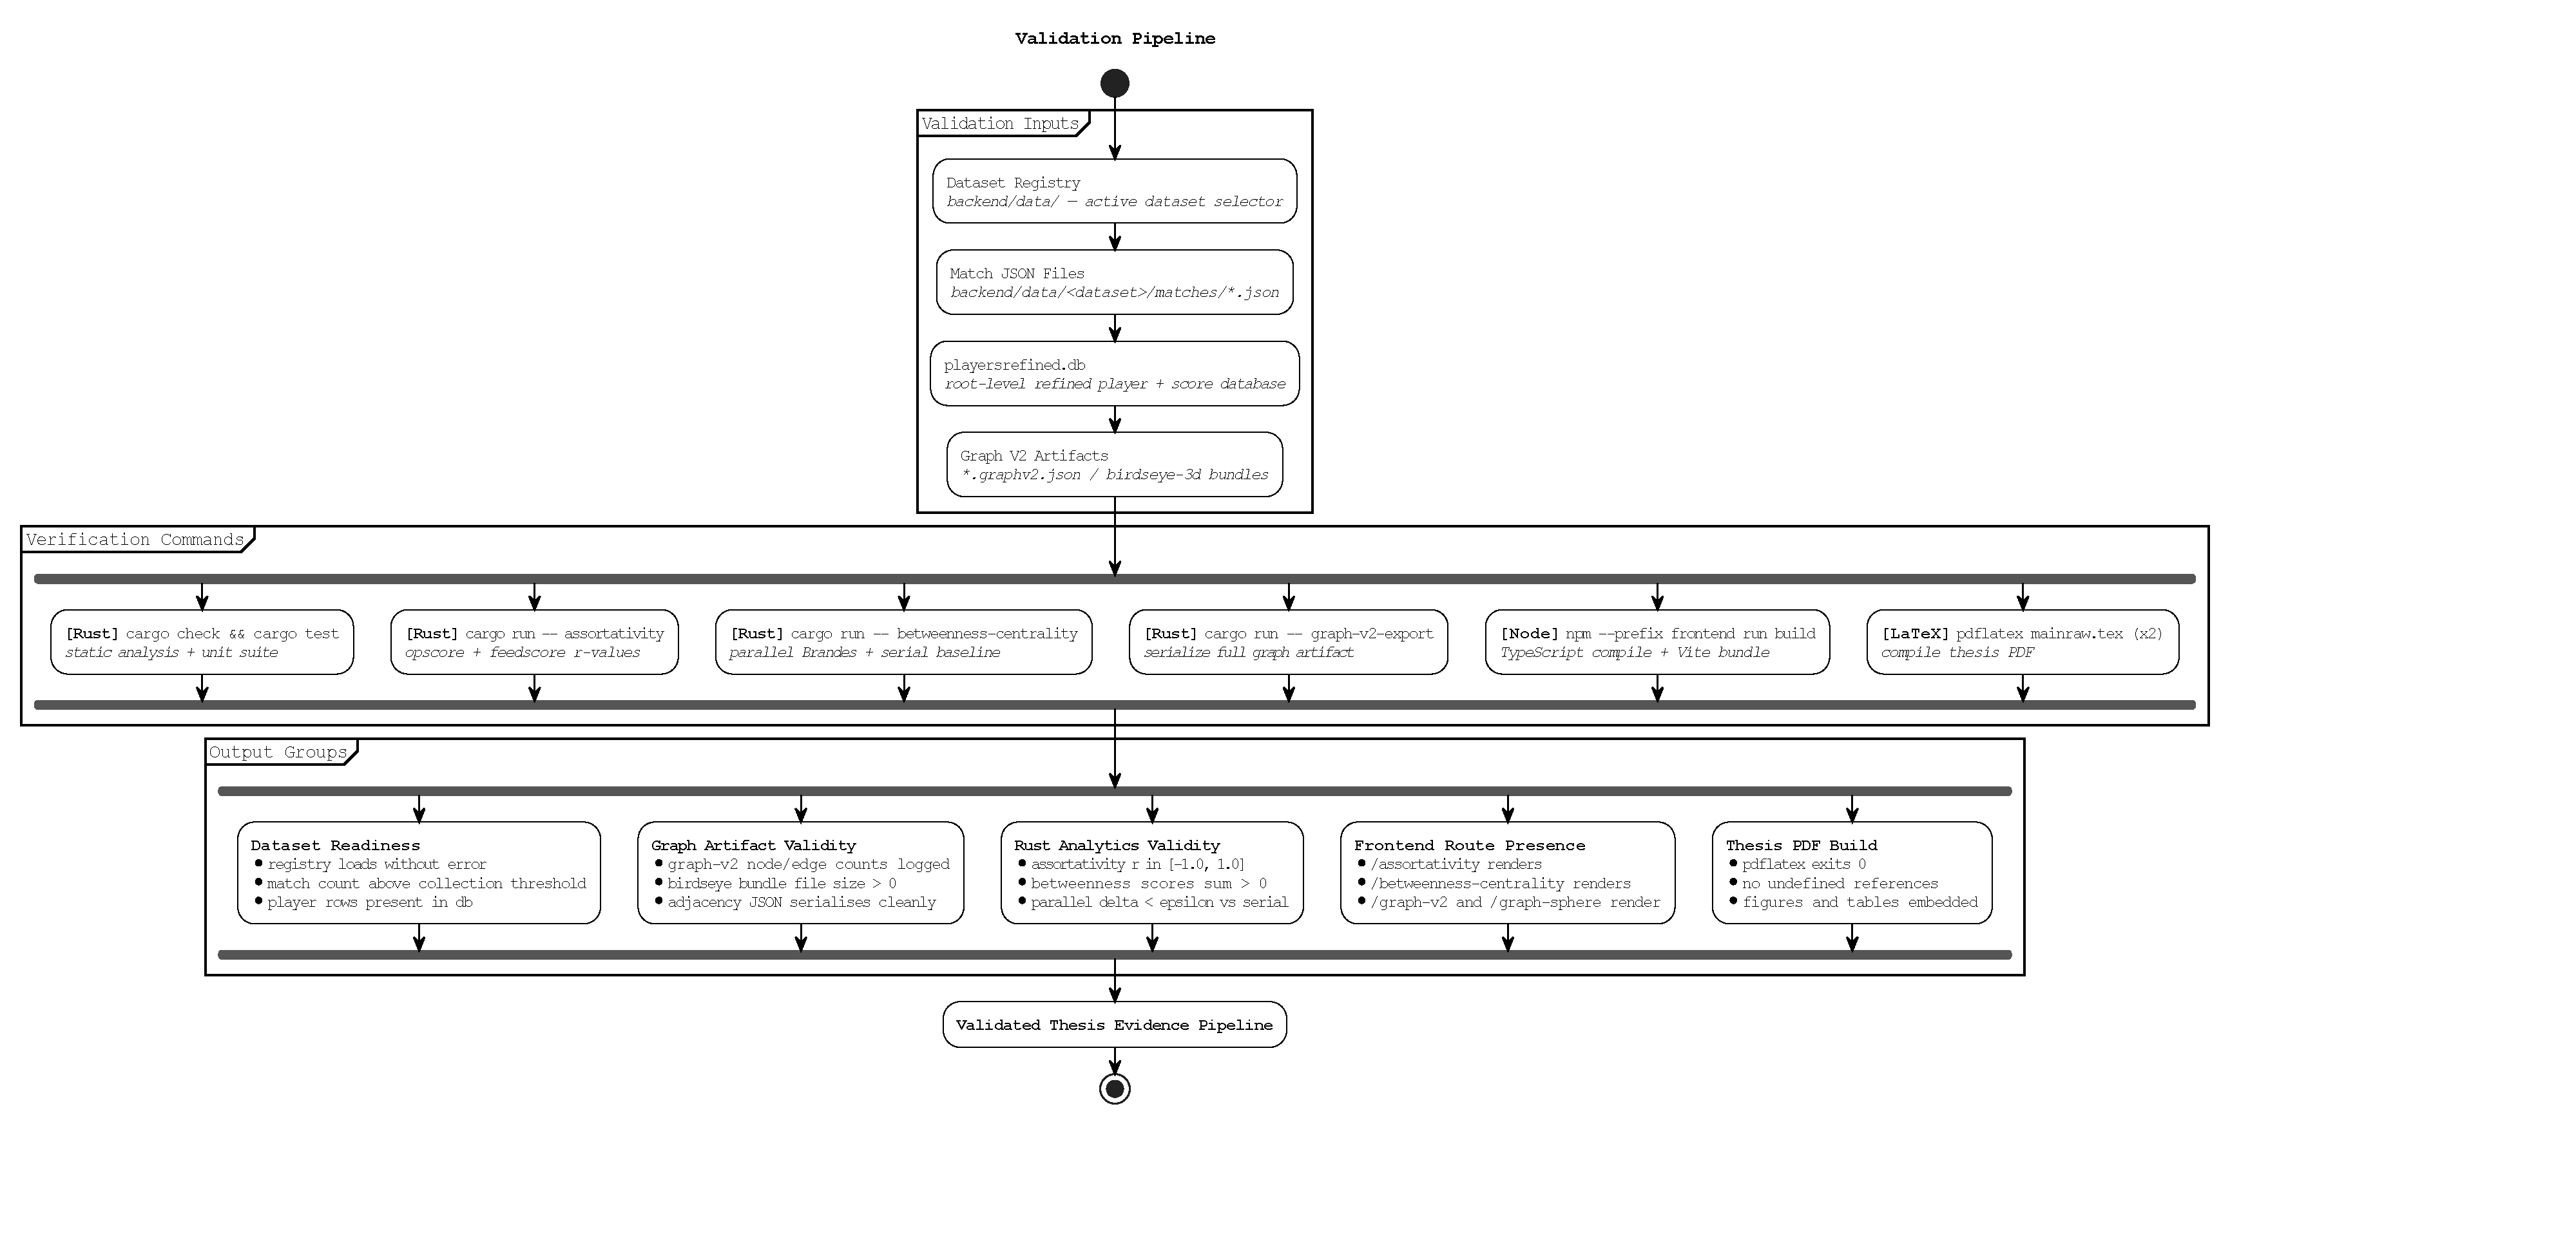
\includegraphics[width=0.98\textwidth,height=0.76\textheight,keepaspectratio]{validation_pipeline.pdf}
\caption{A dolgozati bizonyítékok validációs pipeline-ja a \texttt{thesis-validation-pipeline.puml} forrás alapján. A diagram először a validációs bemeneteket mutatja: dataset-regiszter, meccs-JSON állományok, \texttt{playersrefined.db} és Graph V2 artifactok. Ezután párhuzamos ellenőrzési parancsokra bontja a folyamatot: Rust \texttt{cargo check}/\texttt{cargo test}, asszortativitás, Brandes-betweenness, Graph V2 export, frontend build és dolgozati PDF-fordítás. A kimeneti csoportok külön ellenőrzik a dataset-készültséget, a gráfartifactok érvényességét, a Rust analitikák tartomány- és deltafeltételeit, a frontend útvonalak jelenlétét és a PDF build sikerét.}
\end{figure}

% ===== chapters/19-rendszerszintu-ertekeles-es-megvitatas.tex =====
\chapter{Rendszerszintű értékelés és megvitatás}

\section{Mi bizonyult a legerősebb rendszertervezési döntésnek?}

Az egész projektet visszanézve a legerősebb döntésnek azt tartom, hogy a különböző feladatokat nem próbáltam egyetlen univerzális technológiába kényszeríteni. A rendszer nem eszközpreferencia, hanem minőségi attribútumok mentén fejlődött. A fontos attribútumok a következők voltak:

\begin{itemize}
    \item reprodukálhatóság,
    \item magyarázhatóság,
    \item perzisztencia,
    \item futási teljesítmény,
    \item demo- és védhetőségi koherencia.
\end{itemize}

Ezek közül ritkán lehet mindent ugyanazzal az eszközzel a legjobban kiszolgálni. A Python gyors iterációt és kényelmes adatfeldolgozást ad, a Rust teljesítményt és pontos gráfkontrollt, a Node/Express stabil integrációs felületet, a React pedig erős bemutathatóságot. A többnyelvűség tehát itt nem öncélú komplexitás, hanem funkcionális specializáció.

\clearpage
\begingroup
\special{papersize=210mm,430mm}
\special{pdf:put @thispage << /MediaBox [0 0 595.276 1218.898] >>}
\section{A rendszer erősségei}
\enlargethispage{150mm}

\begin{figure}[H]
\centering
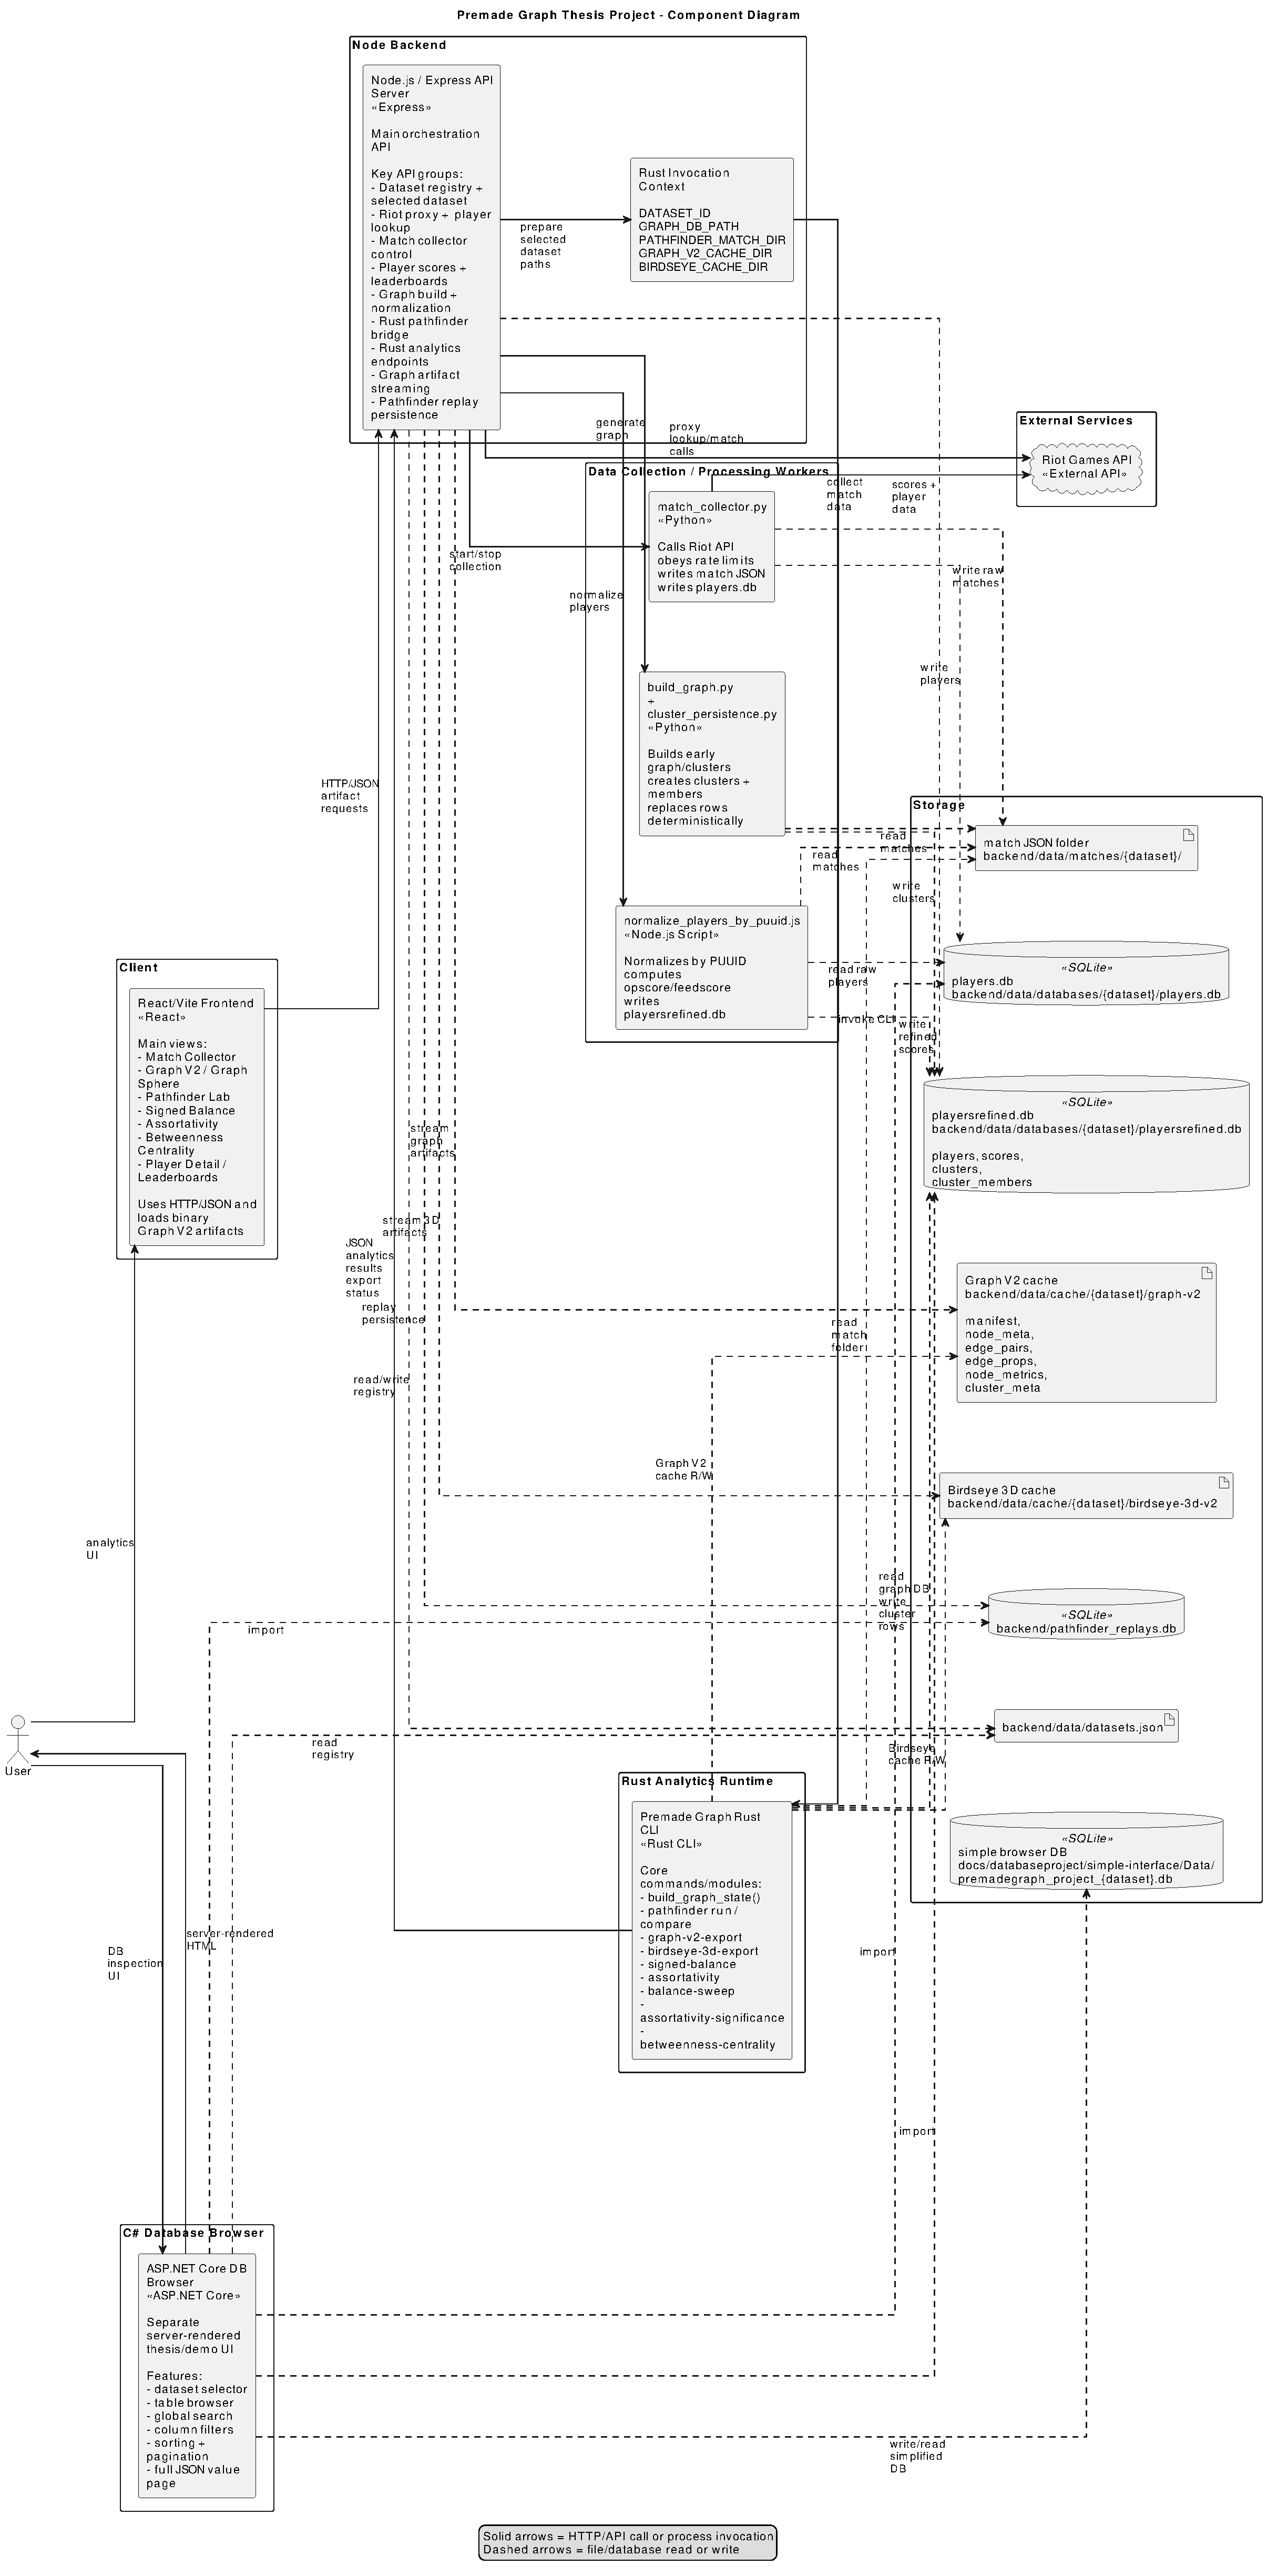
\includegraphics[width=0.98\textwidth,height=330mm,keepaspectratio]{full system diagram.pdf}
\caption{A teljes rendszer komponensdiagramja - az adatút a Riot API-tól a React frontendig}
\end{figure}
\clearpage
\endgroup
\special{papersize=210mm,297mm}

A jelenlegi állapot alapján a projekt legfontosabb erősségei:

\begin{itemize}
    \item a teljes adatút végigkövethető a Riot API-tól a frontendig;
    \item a játékosprofilok explicit, ellenőrizhető képleteken és mezőkön alapulnak;
    \item a gráfépítés és klaszterezés nem csak vizuális export, hanem perzisztens objektum;
    \item a Rust réteg valódi analitikai és futtatási értéket ad, nem csak ``gyorsabb átírás'';
    \item az asszortativitás, a core-periphery gráfolvasat és a Brandes-központiság valódi kutatási kérdésekké emelik a rendszert.
\end{itemize}

\section{Fenyegetések a validitásra}

Egy védhető szakdolgozatban legalább ennyire fontos kimondani a korlátokat is. A jelen projekt legfontosabb validitási kockázatai:

\begin{itemize}
    \item a dataset nem reprezentálja a teljes játékospopulációt;
    \item a gyűjtés seed- és queue-függő;
    \item a \texttt{feedscore} és \texttt{opscore} interpretálható, de nem ``igazságmérő'';
    \item a signed-balance eredménye nem kap fő empirikus szerepet, mert az enemy-él negatív társas kötésként való értelmezése nem elég erős;
    \item a country-ág sokkal bizonytalanabb, mint a közvetlen gráf- és meccsanalitika.
\end{itemize}

Ezek a korlátok azonban nem rombolják le a dolgozatot. Inkább kijelölik azt a határt, amelyen belül az állítások védhetők. Ezért is volt fontos, hogy a megvalósult és a jövőbeli elemeket szigorúan külön kezeljem.

Érdemes a validitási kockázatokat rétegenként is szétbontani:

\begin{itemize}
    \item \textbf{Mintavételi validitás}: a seedválasztás, a premade-probe és a queue-orientáció együtt nem véletlen mintát adnak a teljes játékospopulációból.
    \item \textbf{Mérési validitás}: a \texttt{feedscore} és \texttt{opscore} értelmezhető, de konstrukciós döntésekre épülő metrikák; különösen az \texttt{opscore} tartalmaz kézi szerepkör-súlyozást.
    \item \textbf{Projekciós validitás}: a gráfmód, az élküszöb és az ally/enemy kapcsolatértelmezés érdemben alakítja a végső analitikai mintát; a signed-balance emiatt csak módszertani határesetként használható.
    \item \textbf{Klasztervaliditás}: a közösségdetektálás eredménye függ a választott gráftól, a küszöböléstől és a modularitás felbontási korlátjától \cite{fortunato_barthelemy2007}.
    \item \textbf{Időbeli validitás}: a korpusz fokozatosan épülő archívum, ezért a teljes háló nem egyetlen szinkron időpillanat felvétele.
\end{itemize}

Ezek a fenyegetések azonban nem cáfolják a projektet. Inkább megmutatják, hogy meddig lehet erős állításokat tenni, és hol kell tudatosan visszafogni az interpretációt. A dolgozat védhetőségét végső soron éppen ez a rétegzett őszinteség erősíti.

\section{Miért értékes a projekt szakdolgozatként?}

Szakdolgozati szempontból a projekt értéke nem csak abban áll, hogy ``sok mindent tud''. A valódi érték az, hogy több informatikai terület kapcsolódik össze benne:

\begin{itemize}
    \item adatgyűjtés és API-használat,
    \item adatbázistervezés,
    \item hálózatkutatás,
    \item algoritmusok és teljesítmény,
    \item frontend és vizuális kommunikáció.
\end{itemize}

Ez a kombináció azért erős, mert minden réteg hozzájárul a végső állításhoz. Ha bármelyik hiányozna, a dolgozat jóval gyengébb lenne: pusztán frontendként látványos lenne, pusztán algoritmusként kontextustalan, pusztán adatelemzésként pedig bemutatási réteg nélkül maradna.

Ehhez hozzáadódik a reprodukálhatósági érték is. A rendszer fő eredményei nem kézzel összeollózott prezentációs pillanatképekből állnak, hanem olyan pipeline-okból, amelyek a nyers meccs-JSON-tól a normalizált játékosprofilon és a perzisztált klasztereken át a Rust-analitikáig követhetők. Ez különösen erős szakdolgozati tulajdonság: a bemutatott állításokhoz tartozik egy végrehajtható technikai út is.

\section{A megvalósult és a jövőbeli elemek szétválasztása}

A dolgozat egyik tudatos módszertani döntése az volt, hogy a jelenleg implementált és a még csak tervezett elemeket nem keverem össze. A jelenlegi, ténylegesen megvalósult mag a következő:

\begin{itemize}
    \item Riot API-ra épülő adatgyűjtés;
    \item \texttt{puuid}-alapú normalizálás;
    \item \texttt{feedscore}/\texttt{opscore} számítás;
    \item legacy Python export és populációs közösségdetektálás;
    \item SQLite klaszterperzisztencia;
    \item Rust Graph V2 gráfépítés, útvonalkeresés, asszortativitás, központiság és 3D globális export;
    \item asszortativitás és betweenness-központiság.
\end{itemize}

A jelenleg megvalósult mag tartalmazza a databaseproject és C\# böngésző alprojektet is, amely formálisan nem a főrendszer része, de valódi, futtatható eszközként él a repositoryban.

Visszavont irányok (a korábbi tervdokumentumokban szerepeltek, jelenleg nem aktívak): temporal consistency/stabilitás és community cohesion vs. performance vizsgálat eltávolítva a jelenlegi scope-ból. A Brandes-központiság ezzel szemben már implementált modul, amelynek további feladata nem az alapalgoritmus megírása, hanem a benchmarkolás és a Graph V2 artifact-rétegbe illesztés.

Ez a szétválasztás nem gyengíti, hanem erősíti a dolgozatot. A bírálat szempontjából sokkal védhetőbb egy olyan szöveg, amely pontosan kijelöli a rendszer jelenlegi határát, mint egy olyan, amely minden jó ötletet kész eredménynek próbál feltüntetni.

% ===== chapters/20-a-ket-adatkeszlet-empirikus-osszehasonlitasa-flexset-versus-soloq.tex =====
\chapter{A két adatkészlet empirikus összehasonlítása: \texttt{flexset} versus \texttt{soloq}}

\section{Miért szükséges a két adatkészlet összehasonlítása?}

A projekt egyik legfontosabb kutatási-módszertani döntése az volt, hogy nem egyetlen adatkészlettel dolgozik, hanem egymással összehasonlítható, eltérő queue-szemantikájú korpuszokkal. Ez nem pusztán mennyiségi bővítés, hanem kvalitatív különbségtétel: a \texttt{flexset} (EUNE Master$+$ Flex Queue) és a \texttt{soloq} (EUNE Master$+$ Solo/Duo Queue) nemcsak méretükben, hanem a bennük keletkező kapcsolatok jellegében is eltérnek.

A kutatási kérdés így fogalmazható meg: ha ugyanazon analitikai pipeline-t lefuttatjuk mindkét dataseten, mikor kapunk eltérő eredményt, és ez az eltérés értelmezhető-e a két queue eltérő mechanikájából?

A \textbf{research-workflow} szemlélet szerint ez az összehasonlítás nem utólagos illusztráció, hanem a módszertan integráns része. Az egyetlen datasetre épülő eredmény interpretálása mindig kétséges: az eredmény lehet a módszer hatása, lehet a dataset sajátossága, vagy lehet valódi gráfstruktúra. Két, eltérő generáló mechanizmussal bíró dataseten kapott konvergens vagy divergens eredmény sokkal erősebb támpontot ad.

\section{A két dataset konstruktív különbségei}

\subsection{Queue-szemantika és kapcsolatgeneráló mechanizmus}

A Flex Queue (440-es queue ID) csapatszedést tesz lehetővé: játékosok 2--5 főig premade csapatot alkothatnak, és egységként lépnek be a meccsbe. Ez azt jelenti, hogy a szövetségesi pozícióban repeatedly megjelenő játékospárok egy része \emph{szándékolt ismétlődés}: a premade csapat azonos tagjai meccsről meccsre együtt indulnak. Az ally/enemy arány (73.17\% ally a flexseten) részben ennek a mechanizmusnak a következménye.

A Solo/Duo Queue (420-as queue ID) ezzel szemben legfeljebb két fős premade-et engedélyez. A matchmaking itt jóval véletlenszerűbb: egy adott játékos öttagú csapatának többi tagja döntően nem szándékolt, hanem algoritmikus összerendelés. Az ally/enemy arány (65.24\% ally a soloq-on) alacsonyabb, ami összhangban van azzal, hogy a véletlenszerűbb meccsek kevesebb domináns szövetségesi kapcsolatot hoznak létre.

\subsection{Adatskála és meccssűrűség}

\begin{table}[H]
\centering
\caption{A két dataset alapvető méretei}
\begin{tabularx}{\textwidth}{>{\raggedright\arraybackslash}p{5cm} rr}
\toprule
\textbf{Mutató} & \textbf{flexset} & \textbf{soloq} \\
\midrule
Meccs-JSON állományok & 4981 & 2001 \\
Nyers játékosok & 15\,147 & 2822 \\
Finomított játékosok & 15\,421 & 6768 \\
Klaszterek (DB) & 599 & 140 \\
Klasztertagok (DB) & 5741 & 1538 \\
Graph V2 látható csúcsok & 5741 & 1538 \\
Graph V2 látható élek & 18\,548 & 4111 \\
Átlagos élsúly & 3.405 & 2.364 \\
Graph V2 ally/enemy arány & 73.17\% / 26.83\% & 65.24\% / 34.76\% \\
Graph V2 klaszterek & 1531 & 870 \\
Átlagos klaszterméret & 3.750 & 1.768 \\
Legnagyobb klaszterméret & 20 & 20 \\
\bottomrule
\end{tabularx}
\end{table}

Az átlagos élsúly különbsége (3.405 vs. 2.364) különösen figyelemreméltó. Ez azt jelenti, hogy a flexset-en a látható kapcsolatok átlagosan sűrűbb, ismétlődőbb előfordulásból épülnek fel. Ahol a soloq-on egy él két meccs ismétlődéséből áll össze, ott a flexset-en tipikusan több mint három meccs van mögötte. Ez közvetlen mérőszáma annak, hogy a Flex Queue-ban az azonos játékospárok egymással sűrűbben, tartósabban találkoznak.

\section{A két dataset vizuális klaszterstruktúrájának különbsége}

Az átlagos klaszterméret különbsége (3.750 vs. 1.768) szintén tartalmas. A flexset-en a csoportok átlagosan majdnem négytagúak, míg a soloq-on szinte mindenütt kis, kétfős vagy egyedülálló klaszterek dominálnak. Az 1.768-as átlag azt jelenti, hogy a soloq-ban a Graph V2 által látható csomópontok közel fele egyedül álló csúcs (azaz nincs mellette kellő súlyú szövetségesi partner).

Ez a különbség nem adatgyűjtési hiba, hanem a queue-mechanika közvetlen következménye. A premade Flex Queue-ban természetesen keletkeznek 3--5 fős, ismétlődő klasztermagok, amelyek a Graph V2-ben összefüggő csoportként jelennek meg. A véletlenszerűbb soloq-ban ez a csoportosulás nem jön létre organikusan.

A bridgecandidateClusters és outerOrbitClusters értékei is különböznek: a flexseten 815 bridgejelölt-klaszter van 1531 összesből (53.2\%), a soloq-on 605 jelölt 870-ből (69.5\%). Ez meglepő arány - a soloq klaszterei relatíve több hidat képeznek. Ennek magyarázata valószínűleg az, hogy a soloq-on a kis klaszterek jobban szétszórtabb, kevésbé összefüggő grafikonban helyezkednek el, így relatív módon több közöttük a vizuálisan kitüntetett pozícióban lévő.


\section{A metrikafedettség összehasonlítása}

Mindkét dataseten a Graph V2 artifact teljesen fedett opscore és feedscore értékekkel:

\begin{itemize}
    \item \textbf{flexset}: opscore-fedettség 5741/5741, feedscore-fedettség 5741/5741
    \item \textbf{soloq}: opscore-fedettség 1538/1538, feedscore-fedettség 1538/1538
\end{itemize}

A teljes fedettség azt jelenti, hogy a Graph V2-ben megjelenő minden látható csomóponthoz rendelkezésre áll érvényes opscore és feedscore. Ez az asszortativitási és a gráf-alapú elemzések szempontjából kritikus: nincs olyan csomópont, amely hiányzó score miatt kiesne az elemzésből.

Az opscore átlagok közel esnek egymáshoz: flexset 6.1015, soloq 6.1701. Ez megerősíti, hogy a kétdataset-összehasonlítás az összehasonlíthatóság feltételei között zajlik.

\section{A teljes összehasonlítás tanulságai}

\begin{table}[H]
\centering
\caption{A két dataset összehasonlítás összefoglalója}
\begin{tabularx}{\textwidth}{>{\raggedright\arraybackslash}p{5cm} X X}
\toprule
\textbf{Dimenzió} & \textbf{flexset} & \textbf{soloq} \\
\midrule
Queue-mechanika & Flex, premade-fókusz & Solo/Duo, egyénközpontú \\
Átlagos élsúly & 3.405 (sűrűbb) & 2.364 (ritkább) \\
Ally arány & 73.17\% & 65.24\% \\
Átlagos klaszterméret & 3.750 & 1.768 \\
Triádok/csomópont & 4.95 & 1.03 \\
Core-periphery olvasat & Hídgazdag asszociatív mag és sok periférikus ally-sziget & Kisebb, véletlenszerűbb lokális csoportok \\
Social-path opscore assz. & 0.2346 & 0.1750 \\
Battle-path opscore assz. & 0.1461 & 0.1625 \\
Feedscore battle-path assz. & $-0.0108$ & $-0.0366$ \\
Kutatási szerep & Asszociatív gráf és teljesítménykapcsolat & Teljesítmény-alapvonal, kontroll \\
\bottomrule
\end{tabularx}
\end{table}

Az összehasonlítás általános tanulsága: a \texttt{flexset} az asszociatív játékosgráf és a visszatérő szövetségesi kapcsolatok természetesebb terepe, a \texttt{soloq} pedig a teljesítmény-alapvonal és a kontroll-dataset szerepét tölti be. Ahol a két dataset hasonló eredményt ad (pl. mindkettőn pozitív social-path opscore asszortativitás), ott az eredmény általánosabb jellegű. Ahol eltérnek (pl. klaszterméret, élsűrűség, bridge-orbit szerkezet), ott az eltérés a queue-mechanikából fakad, és önmagában is tudományosan értelmezhető.

Figyelemreméltó részlet a táblázatban: a \texttt{battle-path opscore} értéke a soloq-on \emph{magasabb} (0.1625), mint a flexset-en (0.1461). Ennek magyarázata a soloq szűk MMR-sávján alapuló matchmaking: az ismétlődően egymással találkozó játékosok opscore-ban közel esnek egymáshoz, de ez a struktúra gyengébb és esetlegesebb, mint a flexset szándékolt premade-kapcsolatai. A \texttt{social-path} módban a flexset erősebbebb (0.2346 vs. 0.1750), ami a premade-szövetségesi mechanizmust tükrözi.

% ===== chapters/21-adatbazis-engineering-databaseproject-es-csharp-bongeszo.tex =====
\chapter{Az adatbázis-engineering kiegészítő alprojekt: databaseproject és C\# böngésző}

\section{A kiegészítő alprojekt szerepe és motivációja}

A Premade Graph fő rendszere SQLite-alapú perzisztenciával dolgozik, és a gráfanalitikai pipeline-hoz és a frontendhez optimalizált sémát használ. A \texttt{docs/databaseproject} könyvtárban egy ezzel párhuzamos, de önálló alprojekt él: egy formálisan megtervezett, PostgreSQL-re épülő relációs adatbázismodell és egy ASP.NET Core / C\# alapú adatbázis-böngésző alkalmazás. Ez az alprojekt kettős értékkel bír: egyrészt erősíti az adatbázis-tervezés akadémiai oldalát, másrészt valódi, futtatható eszközt biztosít az elemzési eredmények böngészéséhez.

Az \texttt{architecture-decision} szemlélet alapján fontos tisztázni, miért kettő rendszer létezik egymás mellett. Az SQLite-alapú fő rendszer a gráfépítés, az analitika és a demo-pipeline kiszolgálásához optimalizált: egyszerű telepítés, nincs szerverfüggőség, gyors az iteráció. A PostgreSQL-alapú adatbázismodell ezzel szemben a relációs adatbázistervezés akadémiai igényeivel igazodik: tárolt eljárások, triggerek, rekurzív lekérdezések, JSON-mezők, hivatkozási integritás. A kettő nem versenyez egymással, hanem különböző célt szolgál ugyanabban a domainben.

\section{A formális relációs séma}

A \texttt{docs/databaseproject/schema.sql} egy teljes PostgreSQL sémát definiál. A séma tíz főtáblája a következő:

\begin{table}[H]
\centering
\caption{A databaseproject PostgreSQL sémájának táblái}
\begin{tabularx}{\textwidth}{>{\raggedright\arraybackslash}p{4.5cm}X}
\toprule
\textbf{Tábla} & \textbf{Szerepkör a sémában} \\
\midrule
\texttt{players} & Játékosazonosság, összesített pontszámok, szerepkör \\
\texttt{matches} & Meccsszintű adatok, queue, patch, időtartam, győztes \\
\texttt{teams} & Egy meccs két csapata, oldal, objektíva adatok \\
\texttt{match\_participants} & Résztvevői adatok: champion, lane, kills, deaths, assists \\
\texttt{player\_relationships} & Játékos--játékos ally/enemy kapcsolat súllyal \\
\texttt{clusters} & Klaszter metaadatok, típus, algoritmus \\
\texttt{cluster\_members} & Tagsági rekordok, szerepkör-összegzés \\
\texttt{analysis\_runs} & Elemzési futások metaadatai \\
\texttt{performance\_snapshots} & Játékos-teljesítmény pillanatfelvételek futásonként \\
\texttt{path\_queries} & Útkeresési kérések és eredmények \\
\bottomrule
\end{tabularx}
\end{table}

A séma normalizált: a meccsadatok nem ismétlődnek játékosonként, a résztvevői rekord tartalmazza a meccsre vonatkozó joinolt mezőket, a klasztertagság idegen kulcson keresztül kapcsolódik a játékoshoz és a klaszterhez. A \texttt{CHECK} constraintek biztosítják, hogy az \texttt{opscore} és \texttt{feedscore} értékek a $[0,10]$ tartományban maradnak.

\subsection{Nézetek és összetett lekérdezések}

A \texttt{docs/databaseproject/views\_queries.sql} fájl elemző nézeteket és lekérdezéseket tartalmaz. Ezek közé tartoznak:
\begin{itemize}
    \item \textbf{Szerepkörös teljesítményvizsgálat}: aggregált opscore/feedscore elemzés szerepkörönként;
    \item \textbf{Klaszterösszegzők}: belső sűrűség, hídjátékos-jelzők, átlagos teljesítmény klaszterenként;
    \item \textbf{Kapcsolat-erősségi rang}: a legerősebb ismétlődő ally/enemy pár keresése;
    \item \textbf{Teljesítménystabilitás időben}: teljesítmény-pillanatfelvételek összehasonlítása elemzési futásonként;
    \item \textbf{JSON-alapú metaadat-lekérdezések}: a klaszter \texttt{summary\_json} és \texttt{role\_json} mezőinek lekérdezése PostgreSQL JSON operátorokkal.
\end{itemize}

\subsection{Tárolt eljárások és triggerek}

A \texttt{docs/databaseproject/procedures\_triggers.sql} tárolt eljárásokat és triggereket definiál. Ezek közé tartoznak:
\begin{itemize}
    \item \textbf{Pontszámfrissítési trigger}: meccs-résztvevő beírásakor automatikusan frissíti az aggregált player-szintű opscore-t;
    \item \textbf{Klaszterépítési eljárás}: adott elemzési futáshoz klaszterező logikát futtat és klasztertagságot rögzít;
    \item \textbf{Útkeresés-naplózó eljárás}: útkeresési kérés és eredmény konzisztens rögzítése;
    \item \textbf{Teljesítménypillanatkép-karbantartó}: elemzési futásonként snapshot-ot ír, megőrizve a longitudinális adatot.
\end{itemize}

Az akadémiai szempont itt az, hogy a tárolt eljárások és triggerek az adatbázis-logikát az alkalmazáslogikától elválasztják: az adatmodellek önállóan karbantarthatók, és az elemzési pipeline nem függhet attól, hogy az alkalmazásréteg helyesen hívja-e meg az aggregálási logikát.

\section{Az ASP.NET Core / C\# adatbázis-böngésző}

A \texttt{docs/databaseproject/simple-interface/} könyvtárban egy ASP.NET Core webalkalmazás él, amelyet a Premade Graph SQLite adatbázisainak böngészésére terveztek. A böngésző \texttt{Program.cs} fájlja mutatja, hogyan épül fel ez az eszköz.

\subsection{Adatbázis-generálás és importálás}

Az alkalmazás indulásakor automatikusan futtatja a \texttt{ProjectImporter.Import()} folyamatot, amely a Premade Graph repositoryban lévő SQLite adatbázisból importál a böngésző saját, projektre generált SQLite állományába:

\begin{itemize}
    \item \texttt{players}: opscore, feedscore, szerepkör, meccsszám;
    \item \texttt{clusters}: klasztertípus, méret, metaadatok;
    \item \texttt{cluster\_members}: tagsági rekordok;
    \item \texttt{replay}: útkeresési mentések;
    \item \texttt{replay\_run}: útkeresési futások.
\end{itemize}

Az import eredménye visszajelzést ad a konzolra és webes hibaoldalon jelzi, ha az importált adatbázis nem elérhető. Ez azt jelenti, hogy a böngésző önállóan indítható, és ha az adatforrás hiányzik, explicit hibaüzenetet ad, nem csendesen üres felületet mutat.

\subsection{Dataset-szelektálás}

Az alkalmazás tudatosan illeszkedik a Premade Graph több-adatkészletes architektúrájához. A \texttt{DatasetCatalog.Load(root)} a repository \texttt{datasets.json} regiszterét olvassa be, és a böngésző minden oldalán URL-paraméterként átadható a kívánt dataset azonosítója (\texttt{?dataset=flexset}, \texttt{?dataset=soloq}).

Ez azt jelenti, hogy egyetlen böngészőpéldány az összes regisztrált adatkészlethez adatbázist tud generálni és megjeleníteni, anélkül hogy a mögöttes SQLite állományokat összekeverne.

\subsection{Táblabögészés, szűrés, lapozás és JSON-nézetek}

A böngésző a következő funkciókat valósítja meg:

\begin{itemize}
    \item \textbf{Táblalistázás}: az összes importált tábla nevének és sorainak megjelenítése;
    \item \textbf{Szűrés}: szövegmező alapú szűrés játékosnévre, szereplőre, klasztertípusra;
    \item \textbf{Lapozás}: nagy táblák esetén oldalanként meghatározott számú sor;
    \item \textbf{Rendezés}: oszlop szerinti növekvő/csökkenő sorrend;
    \item \textbf{Teljes értéknézet}: a \texttt{/database/value} endpoint egy adott cella teljes értékét mutatja meg, különösen hasznos a \texttt{summary\_json} és \texttt{role\_json} típusú, hosszú JSON-oszlopoknál.
\end{itemize}

\subsection{Technikai architektúra}

Az alkalmazás egész programja egyetlen \texttt{Program.cs} fájlban helyezkedik el, minimális top-level statement stílussal. Az ASP.NET Core pipeline konfigurálása, az útvonaldefiníciók és az adatbázis-lekérdezések egységes szerkezetben élnek. A renderelés szerver oldali HTML-generálással történik, nincs JavaScript frontend: a böngésző célja az áttekinthetőség és a bemutathatóság, nem egy SPA-szerű élmény.

A \texttt{Microsoft.Data.Sqlite} NuGet csomag az adatbázis-elérés alapja, amely a SQLite adatbázisokhoz natív, közvetlen hozzáférést biztosít .NET-ből. A kapcsolatfelépítés és a lekérdezések a \texttt{ProjectDatabase} osztályon keresztül vannak absztraháLva, ami megkönnyíti a dataset-váltás és az import-logika szétválasztását.

\section{A kiegészítő alprojekt helye a dolgozatban}

\subsection{Miért valódi alprojekt, nem csak dokumentáció?}

A databaseproject nem puszta papír-terv: a \texttt{schema.sql} futtatható, a \texttt{views\_queries.sql} lekérdezései tesztelhetők PostgreSQL-ben, a C\# böngésző lefordul és futtatható a repository-ból. Ez teszi valódi, védhető mellékprojektté.

Az akadémiai értéke kettős:
\begin{itemize}
    \item \textbf{Adatbázis-tervezési szempontból}: bemutatja, hogyan formalizálható ugyanaz a domainmodell egy erősebb, tárolt logikát támogató adatbázisrendszerben; ez az SQLite-on dolgozó fő rendszer korlátait is megvilágítja.
    \item \textbf{Szoftverarchitektúra szempontból}: demonstrálja, hogy a Premade Graph domain-modellje természetesen leírható relációs sémával, tárolt eljárásokkal és triggerekkel, miközben az alapvető fogalmak (players, clusters, cluster\_members, opscore, feedscore) mindkét adatbázis-környezetben koherensek.
\end{itemize}

\subsection{A C\# böngésző mint prezentációs eszköz}

A C\# böngésző azért is értékes a dolgozat szempontjából, mert lehetővé teszi, hogy a SQLite-ban tárolt elemzési eredmények közvetlenül, táblázatosan és JSON-nézettel ellenőrizhetők legyenek. Ez a reprodukálható kutatás egyik alapkövetelménye: az eredmények nemcsak a frontend vizualizációján láthatók, hanem adatbázis-szinten is auditálhatók \cite{sandve2013}.

\subsection{A databaseproject korlátai}

A databaseproject PostgreSQL-sémája és a fő rendszer SQLite-adatbázisa között nincs automatikus, élő szinkronizáció. A PostgreSQL-modell akadémiai-demonstrációs célt szolgál, nem production-szinkronizációt. Ez explicit módon van dokumentálva a \texttt{docs/databaseproject/documentation.tex} fájlban: ``A beadandó adatbázis-változat PostgreSQL-re készült, mert a feladat tárolt eljárásokat, triggereket, rekurzív lekérdezéseket, JSON mezőket és összetettebb SQL elemzéseket is kér. A tényleges alkalmazás jelenleg SQLite-ot használ helyi perzisztenciára, de a dokumentált modell ugyanazokat a fogalmakat viszi át egy erősebb adatbázisrendszerbe.''

Ez a szétválasztás előny, nem hiba: megmutatja, hogy a szoftvermérnöki döntés (SQLite a fő rendszerben) indokolt a project méretéhez és céljához, miközben az akadémiai adatbázistervezési kompetencia bemutatható a PostgreSQL-modellen keresztül.

\part{Tribal NeuroSim}

% ===== chapters/22-tribal-neurosim-rendszer-es-architektura.tex =====
\chapter{Tribal NeuroSim - Rendszer, Architektúra és Alapok}

\section{Célkitűzés, hatókör és kutatási kapcsolat}
\label{sec:neurosim-24-scope}

A Tribal NeuroSim nem önálló játék, hanem a PremadeGraph gráfelemzési pipeline közvetlen folytatása.
Míg az előző fejezetek a League of Legends meccselőzmények alapján épített játékos-kapcsolati gráfokat elemezték -
klaszterezési módszertan (ld. 10. fejezet) és a két adatkészlet empirikus összehasonlítása (ld. 20. fejezet) révén -,
addig a Tribal NeuroSim ezeket a klaszterprofilokat dinamikus, evolúciós szimulációba viszi tovább.

A kapcsolat szerkezete a következő: a PremadeGraph pipeline minden egyes játékosklasztert
teljesítménymetrikák halmazával jellemez - harci hatékonyság, erőforrás-gazdálkodás, objektívkontroll,
kockázattűrés és csapatkoordináció. Ezek az értékek aggregált klaszterszintű mérőszámokká állnak össze
(\textit{A\_combat}, \textit{A\_resource}, \textit{A\_map\_objective}, \textit{A\_risk}, \textit{A\_team}),
amelyek a Tribal NeuroSim törzseinek iniciális genomszekvenciáját alkotják. Az artifactok
az OpScore és a hozzá kapcsolódó részmetrikák aggregált, klaszterszintre emelt változatai:
a 9.~fejezetben bemutatott teljesítménymetrika adja azt az upstream alapot, amelyből a
szimulációs indulóprofilok létrejönnek.
Az upstream derivációs réteg tehát maga a gráfelemzési eredmény: minden szimulált törzs valódi
meccselőzményből levezetett klaszterprofil alapján indul el, nem mesterségesen megkonstruált paraméterekkel.

A szimulációban egyidejűleg mindkét adatkészlet - a Flex Queue és a SoloQ - klaszterei megjelennek.
Ez a közös versenyterep az alapja a kísérlet komparatív értékének: ha az összes törzs azonos
környezeti szabályok alatt küzd erőforrásokért, területért és túlélésért, akkor megfigyelhető,
hogy a strukturálisan eltérő klaszterprofilok eltérő viselkedési stratégiákat fejlesztenek-e ki.
A kutatási kérdés tehát a következőképpen fogalmazható meg:
\textit{ha Flex Queue-ból és SoloQ-ból derivált klaszterprofilok azonos szimulációs szabályrendszer
alatt versenyeznek, vajon a mögöttes gráfstruktúra mérhető különbséget idéz-e elő az emergáló
túlélési stratégiákban?}

A kísérlet kerete exploratív transzfer-vizsgálat \cite{bonabeau2002}.
Nem kísérel meg közvetlen előrejelzést valódi meccskimenetelekre, és nem állít fel
pszichológiai vagy szociológiai kauzalitást a játékosok viselkedése és a szimulációs eredmények között.
A szimuláció egy modell - explicit feltételezésekkel, meghatározott szabályokkal és reprodukálható
seed-alapú futtatásokkal. Az eredmények tehát nem a valóság közvetlen leképezései, hanem
a választott modell viselkedésének megfigyelései.

Ezen határ explicitálása nem gyengesége a megközelítésnek, hanem annak tudományos erőssége.
Az ágensorientált modellezés irodalmában ez bevett módszertani álláspont: a szimulációs kísérletek értékét
éppen az adja, hogy az összehasonlítás feltételrendszere kontrollált és reprodukálható: azonos
szabályok, azonos kezdeti erőforrás-elosztás, determinisztikus seed-ek.
Az ilyen keretben kapott eredmény - \textit{a flexset klaszterprofilok konvergens stratégiát produkálnak,
a soloq klaszterprofilok változékonyabbat} - a modell viselkedéseként értelmezhető és igazolható,
nem pedig spekulatív általánosításként.

A fejezet hátralévő részei ezt az architektúrát bontják ki: a többügynök-modell és az emergencia
mechanizmusa (22.2), az eseményvezérelt megfigyelhetőség (22.3), a rendszerarchitektúra és
teljesítmény (22.4), valamint a build- és telepítési folyamat (22.5).

\section{Ágensorientált és többügynök-modell}
\label{sec:neurosim-24-abm-mas}

\subsection*{Ágensorientált modellezési keret}

A Tribal NeuroSim ágensorientált modell (ABM): minden törzs önálló döntéshozó egység,
amely kizárólag saját lokális állapota és közvetlen térbeli környezete alapján cselekszik.
Nincs globális optimalizáló, nincs központi irányítás, nincs olyan mechanizmus,
amely a végkimenetelt előre definiálná. A makroszintű minták - terjeszkedés, háborúk,
birodalomkialakulás, kihalás, konszolidáció - kizárólag az egyéni döntések összegzéseként
jelennek meg \cite{bonabeau2002}.

Ez a felépítés szándékos. Az ABM paradigma éppen azt teszi vizsgálhatóvá,
amit a klasszikus analitikus modellek nem: hogyan keletkeznek komplex struktúrák
egyszerű, lokális szabályokból. Egy törzs, amely alacsony élelmiszerkészletére reagálva
szomszédos tile-t igényel, nem „birodalmat épít" - csupán lokálisan racionálisan cselekszik.
A birodalom az ezres nagyságrendű ilyen döntés emergens következménye.

\subsection*{Többügynök-rendszer: decentralizált entitások}

A rendszer többügynök-rendszerként (MAS) is értelmezhető \cite{wooldridgejennings1995}:
minden törzs önálló ágensként működik saját belső állapottal (genomszekvencia, populáció,
élelmiszer, területi kiterjedés, aktív háborúk listája), saját lokális percepcióval
(szomszédos tile-ok biome-ja és tulajdonosa, legközelebbi ellenfél és szövetséges távolsága),
és saját döntési logikával (neurális hálózat, amely a bemeneti jelekből viselkedési hajtóerőket
számít). Az ágensek között nincs közvetlen kommunikáció: interakció kizárólag a közös
térbeli szubsztráton keresztül zajlik - területigénylés, háborúindítás, szövetségajánlat.

Hangsúlyozandó, hogy a törzsek \textit{nem} egyéni játékosokat reprezentálnak.
Minden törzs egy teljes játékosklasztert testesít meg populáció-szintű ágensként:
az iniciális genomszekvenciája az adott klaszter aggregált teljesítményprofilja,
nem pedig egyetlen játékos statisztikája. Ez a skálázási döntés összhangban van
a PremadeGraph upstream rétegének klaszter-alapú elemzési szintjével,
amelyet a 10. fejezet részletez.

\subsection*{Emergáló fázisok a konkrét futtatásokból}

A szimuláció lefolyása minden futtatásban azonos szerkezetű fázisokat mutat,
amelyek nem kódoltak előre, hanem a dinamikából következnek.

Az \textbf{első fázisban} (korai terjeszkedés, kb. tick~0-300) 599 törzs szétszórtan
indítja el területigénylését a hex-rácson. A verseny eleinte implicit: a törzsek
nem egymás ellen harcolnak, hanem a szabad tile-okért versengenek. Az erőforrás-gazdag
biome-ok közelében gyorsabban növekszik a populáció, ami hamarabb éri el a polity-fejlesztési
küszöböket (Tribe → City → Duchy → Kingdom → Empire).

A \textbf{második fázisban} (konszolidáció, kb. tick~300-1000) az erősebb törzsek
fokozatosan felszámolják a gyengébbeket. Háborús deklarációk sűrűsödnek, a túlélők
száma drasztikusan csökken. Az F2 korai futtatás adatai ezt a fázist számszerűsítették:
1452 háborút deklaráltak az 1200 tick során, a csúcsaktivitás ~274 egyidejű aktív
háború volt tick=800 körül. A kihalási ráta ugyanekkor érte el maximumát
(74 törzs/100 tick a tick~900-999 ablakban).

A \textbf{harmadik fázisban} (birodalmi háborúk, kb. tick~1000+) csak a legerősebb
polity-szintű entitások maradnak talpon. A map-ot kevés, de kiterjedt Empire-szintű
törzs uralja; a köztük zajló háborúk döntik el a végkimenetelt. Az első teljes futtatásban
(seed=42, flexset) ez a fázis tick=430-ra 121 élőt, tick=853-ra már csak 36 élőt
hagyott meg, mielőtt egyetlen győztes - Tribe 270, Empire szinten - tick=1707-re
átvette az irányítást 6396 tile felett.

\subsection*{Emergáló dinamikák: háborús kaszkád és szövetség-erózió}

A szimulációban két jellegzetes emergáló dinamika figyelhető meg rendszeresen,
amelyek nem szkriptelt eseményekként, hanem a mechanikák természetes következményeként
jelennek meg.

A \textbf{háborús kaszkád} akkor indul, amikor több törzs egyidejűleg érzékeli ugyanazt
az opportunitást: egy meggyengült domináns szomszéd. Mivel minden törzs önállóan,
lokális információk alapján hoz döntést, a deklarációk szinte szimultán zajlanak.
Ez a dinamika különösen markánsan jelent meg a flexset seed=7777 futtatásban,
ahol tick=2040 körül 55 egyidejű opportunista háború tört ki, és a mező 205-ről
13 élőre zsugorodott 200 ticken belül.

A \textbf{szövetség-erózió} az ellentétes irányból hat: két törzs, amely korábban
szövetségesként viselkedett (kölcsönös meg-nem-támadás), az erőforrás-szűkösség
növekedésével felülvizsgálja ezt az egyensúlyt. Mivel a szövetség bináris
(teljes megnemtámadás vagy teljes háború), az átmenet azonnali és visszafordíthatatlan.
A szövetség-erózió mechanizmusa nem jelent meg minden futtatásban azonos intenzitással,
de megfigyelhető volt mind a flexset, mind a soloq datasetből seeded futtatásokban.
Fontos hozzátenni, hogy a végső, javított futásokban formális szövetségek ritkán
jöttek létre. A mechanika jelen van, de a tényleges makrodinamika többnyire
abszorpcióként jelent meg: a gyengébb törzs ellenállással vagy ellenállás nélkül
beolvadt a nagyobb területi struktúrába.

\subsection*{Az F2 futtatás mint korai ellenőrzési pont}

Az F2 futtatás nem a végleges rendszer bizonyítéka, hanem egy korai, hasznos
ellenőrzési pont. Ebben a verzióban már látható volt, hogy a neurális kimenetek nem
maradnak némák: 599 klaszter-derivált törzs, 1200 tick és flexset adatkészlet mellett
mind a 7 kimeneti hajtóerő aktív volt. Ez akkor fontos mérföldkő volt, mert a korábbi
prototípusokban a szimuláció vagy befagyott, vagy úgy futott le, hogy a döntések
nem okoztak érdemi különbséget a törzsek között.

Az F2-ből ezért csak óvatos következtetés vonható le: ezen a ponton a neurális réteg
már működött, a fitneszértékek elkezdtek szétválni, és megjelent a szelekciós nyomás.
Nem állítható viszont, hogy ez a futás igazolta volna a végleges architektúrát. A későbbi,
2026.~május~16-i és 2026.~május~18-i javítási körök után vált fontossá a determinisztikus,
esemény-alapon visszaellenőrizhető futás, ahol a tile-öröklés, a háború alatti
élelmiszergyűjtés, az artifact-diverzitás és a tombstone-audit már a javított szabályok
szerint működött.

\begin{figure}[h]
\centering
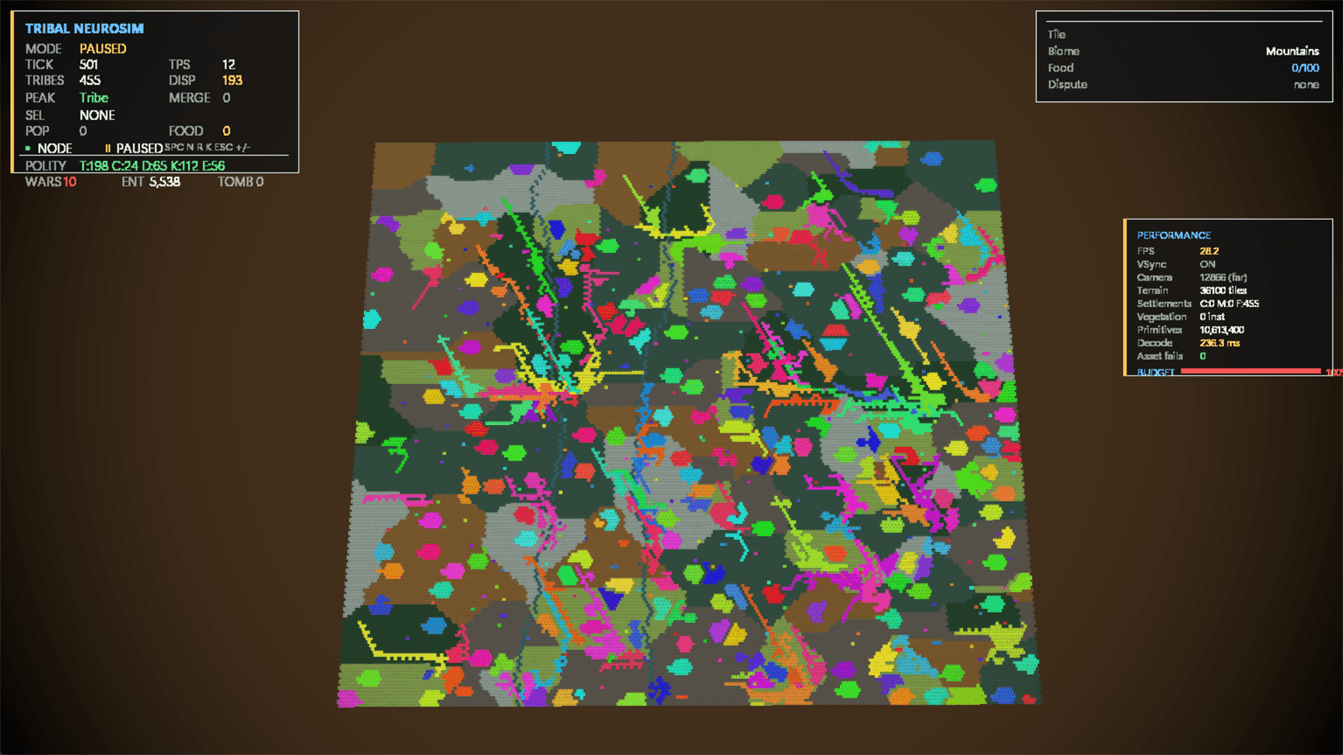
\includegraphics[width=0.9\textwidth]{assets/neurosim/run67fl7777-fl-s7777-tick500.png}
\caption{Flexset seed=7777, tick=500: 455 élő törzs konszolidáció közben.
A területi foltok mérete jelzi az emergáló hatalmi struktúrát.}
\label{fig:neurosim-fl7777-tick500}
\end{figure}

\begin{figure}[h]
\centering
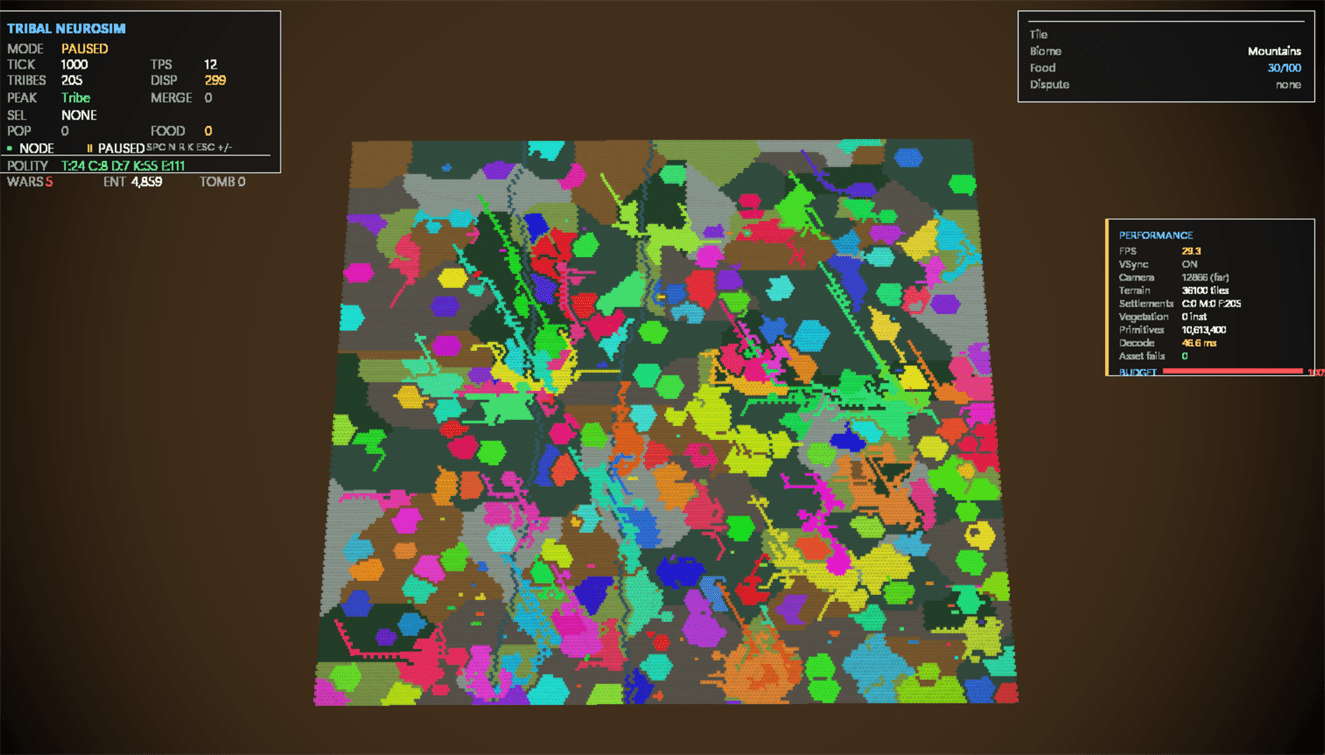
\includegraphics[width=0.9\textwidth]{assets/neurosim/run67fl7777-fl-s7777-tick1000.png}
\caption{Flexset seed=7777, tick=1000: 205 élő törzs, a birodalom-korszak
kezdete. A polity-szint dominanciája látható.}
\label{fig:neurosim-fl7777-tick1000}
\end{figure}

A 20. fejezetben tárgyalt flexset-soloq makroszintű összehasonlítás itt nyer szimulációs
vetületet: az eltérő gráfstruktúrákból derivált klaszterprofilok eltérő emergáló
dinamikákat produkálnak ugyanabban az ABM keretben, ugyanazok alatt a szabályok alatt.

\section{Eseményvezérelt megfigyelhetőség}
\label{sec:neurosim-24-observability}

\subsection*{Miért nem elegendő a végső térképállapot}

Egy szimuláció tudományos értéke nem merül ki a végső állapot rögzítésében.
Annak megállapítása, hogy melyik törzs nyert, önmagában nem magyarázza a nyerés okát.
Ahhoz, hogy egy törzs túlélése, terjeszkedése vagy összeomlása értelmezhető legyen,
minden lényeges állapotváltásnak nyomkövethetőnek kell lennie: melyik tick-en halt éhen,
melyik háborút nyerte, milyen genommal haladt a következő generációba, és miért hagyott
fel egy szomszédos tile igénylésével.

Ez a felismerés a v2 webes prototípus post-mortem elemzéséből következett közvetlenül.
A korai futtatásban tick=187 körül a populáció közel felére zuhant, de a rendszerben
semmiféle nyom nem maradt arról, miért: nem volt rögzítve a kihalás oka, a törzs azonosítója,
az utolsó élelmiszer-állapot, sem az, hogy háborúban halt-e el vagy éhhalál következtében.
Ugyanebben a futtatásban tick=257-re 323 aktív háborút jelzett a rendszer, miközben
a populáció már jóval alacsonyabb volt ennél - ez volt az első mért jele az úgynevezett
\textit{ghost war} problémának: a halott törzsek háborúi nem szűntek meg,
hanem tovább halmozódtak a memóriában.
A végső állapotban, tick=3085-nél, egyetlen élő törzs állt szemben 182 aktív
szellemháborúval. A szimuláció lefutott, de nem volt interpretálható.

Ez a tapasztalat vezette be a kritikus újratervezés egyik sarokköveként az
eseményvezérelt megfigyelhetőség elvét: a szimulációnak minden lényeges eseményt
strukturáltan kell rögzítenie, az append-only eseménybusz elvét követve \cite{fowler2005}.

\subsection*{Append-only eseménybusz és törzsenként napló}

A v3 architektúrában az eseménynapló két rétegből áll.

A \textbf{globális eseménybusz} append-only gyűrűs pufferként működik: minden kihalás,
háborúdeklaráció, szövetségkötés, generációváltás és intervenciós esemény bekerül
egy időrendezett naplóba. A bejegyzések strukturált rekordok: tartalmazzák az esemény típusát,
a tick és generáció számát, az érintett törzs azonosítóját, és ahol releváns, az ellenfél
vagy az érintett tile azonosítóját is. A bejegyzések a \texttt{GET /api/events/recent}
REST endpointon keresztül lekérdezhetők, alapértelmezésként az utolsó 50 bejegyzéssel.

A \textbf{törzsenként napló} minden élő és kihalt törzshöz önálló eseményszálat tart fenn.
A törzs halála nem törli a naplóját: a \texttt{GET /api/tribes/\{id\}/events}
endpoint kihalt törzsek esetén is kiszolgál. Ez az utólagos értelmezhetőség
architektúrájának alappillére: a teljes futtatás után visszakereshető, miért halt ki
az adott törzs, milyen háborúkban vett részt, és melyik genomot vitte magával utolsó generációjáig.

\subsection*{Tombstone rekordok: kihalt törzsek auditálható állapota}

A TaskR2 implementáció bevezette a \texttt{TombstoneLedger} modult.
Minden törzs halálakor egy \texttt{TombstoneRecord} kerül rögzítésre, amely tartalmazza:
a törzs és klaszter azonosítóját, a halál tick-jét és generációját, a populációt és
területet a halál pillanatában, a halál okát (\textit{cause}), a leszármazási összefoglalót,
valamint az öt artifakt-pontszám pillanatfelvételét (\textit{final\_artifacts}).
A rekord mérete ~100 bájt - a kihalt törzs teljes aktív állapotát felváltja
ez a kompakt auditbejegyzés.

A \texttt{cleanup\_tribe()} metódus atomikusan hajtja végre a törzs felszámolását:
tombstone rögzítése, majd az összes aktív háború lezárása \texttt{WarCancelled}
státusszal, végül a területi igények visszavonása. Ez az atomikus végrehajtás
szünteti meg a ghost war jelenséget: a halott törzs háborúi azonnal eltűnnek
az aktív háborúk listájából.

\begin{figure}[h]
\centering
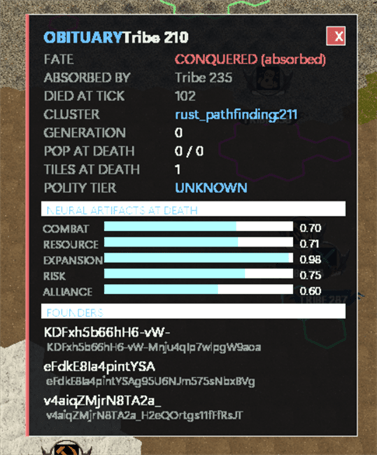
\includegraphics[width=0.82\textwidth]{assets/neurosim/screenshots-orbituary.png}
\caption{Tombstone/obituary nézet: a kihalt törzsek auditálható rekordként maradnak
vissza, nem aktív szimulációs objektumként.}
\label{fig:neurosim-tombstone-obituary}
\end{figure}

\subsection*{Háborús eseménystruktúra}

A TaskL implementáció bevezette a \texttt{WarState} adatstruktúrát, amely egy háborút
teljes életciklusán át nyomon követ. Minden háborús rekord rögzíti a háborút indító
és fogadó törzs azonosítóját, az indulás tick-jét, az aktuális státuszt
(\texttt{Active}, \texttt{Peace}, \texttt{AttackerWon}, \texttt{DefenderWon}),
a felek veszteségeit harci köröként frissítve, valamint az aktuális csatahelyszín tile-azonosítóját.
A \texttt{GET /api/wars/active} endpoint az összes aktív háborút visszaadja
a eltelt tick-szám és kumulált veszteségekkel együtt. A háborúdeklaráció és a kimenetel
(\texttt{WarDeclared}, \texttt{WarResolved}) mind a globális eseménybuszba, mind az
érintett törzsek saját naplójába bekerül.

\subsection*{JSONL napló a fejnélküli CLI futtatásokhoz}

A headless (\texttt{--cli-run}) futtatási módban a szimuláció JSONL formátumú naplót ír
a standard kimenetre. Három típusú bejegyzés váltakozik:
(1)~\texttt{checkpoint} rekordok konfigurálható tick-intervallumonként - tartalmazzák
az élő törzsek számát, az aktív háborúkat, a polity-eloszlást és az aggregált
fitnesz-statisztikákat;
(2)~háborús esemény rekordok minden deklarációra és kimenetelre;
(3)~egyetlen \texttt{final\_summary} bejegyzés a futtatás végén - rögzíti a győztest,
annak genomprofilját, viselkedési archetípusát, a teljes háborús mérleget, és
az összes kihalt törzs tombstone-összesítőjét.

Ez a napló teszi lehetővé a batch futtatások determinizmus-igazolását: öt párhuzamos
fejnélküli futtatás azonos seed-del azonos \texttt{final\_summary} győztes rekordot kell
produkáljon, és ez az egyezés mérhetően ellenőrizhető.

A végjáték értelmezéséhez a térképkép helyett a napló a döntő forrás. A seed=42
flexset futás friss, javított logja például tömören mutatja, hogy a végső szakaszban
nem szövetségi egyensúly, hanem egymást követő abszorpciók és háborús lezárások vezettek
az egyetlen túlélőhöz:

\begin{lstlisting}[language={},caption={Flexset seed=42 végjáték-részlet a javított futás logjából}]
[SIM tick=2400] alive=3 tiles=39368 max_tile=23149 avg_pop=1419769 wars_active=2
[WAR tick=2424] tribe_596 defeated tribe_557 (attacker won)
[SIM tick=2450] alive=2 tiles=39368 max_tile=28161 avg_pop=1314475 wars_active=0
[OPPORTUNITY WAR tick=2460] tribe_90 -> tribe_596 (raid=0.28 aggr=0.84)
[WAR tick=2487] tribe_596 defeated tribe_90 (attacker won)
\end{lstlisting}

\section{Rendszerarchitektúra és teljesítmény}
\label{sec:neurosim-24-architecture}

\subsection*{Hatáskör-megosztás: Rust, C\# MonoGame és Node}

A Tribal NeuroSim v3 háromkomponensű architektúrán alapul, ahol minden réteg
felelősségi köre explicit szerződésben rögzített, és az átfedések szándékosan kerültek.

A \textbf{Rust futtatókörnyezet} az autoritás egyetlen forrása: a tick-ciklust,
a világállapotot, a törzsek neurális döntéshozatalát, a háború- és szövetségfeloldást,
a fuzionálási logikát, a leszármazási regisztert, a tombstone-bejegyzéseket
és az eseménynaplózást mind a Rust bináris kezeli \cite{jung2020}.
Sem a C\# kliens, sem a Node közvetítőréteg nem tart fenn párhuzamos
szimulációs szabályrendszert éles futtatás esetén.
Ez a döntés a 12. fejezetben ismertetett Rust-futtatókörnyezeti elvek közvetlen
kiterjesztése a szimulációs tartományra.

A \textbf{C\# MonoGame kliens} kizárólag vizualizáció és operátori felület:
kamera, térkép-renderelés, törzsinspekciós panel, HUD, artifact-sávok, háborús jelzők.
A kliens nem igazságforrás - a Rust által szolgáltatott keretadatot jeleníti meg,
és lokális demó-harnesszel rendelkezik vizuális teszteléshez (\texttt{--empire-stress},
\texttt{--dispute-stress}), de ez nem a valódi termék futtatási útja.

A \textbf{Node réteg} vékony közvetítő: összekötőhíd a MonoGame és a Rust szerver
között, dataset-export, indítási konfiguráció és batch-orchestráció kezelője.
Szimulációs logikát nem tartalmaz; minden parancsot és keretfolyamot változtatás nélkül
proxyzik a Rust felé.

\begin{figure}[h]
\centering
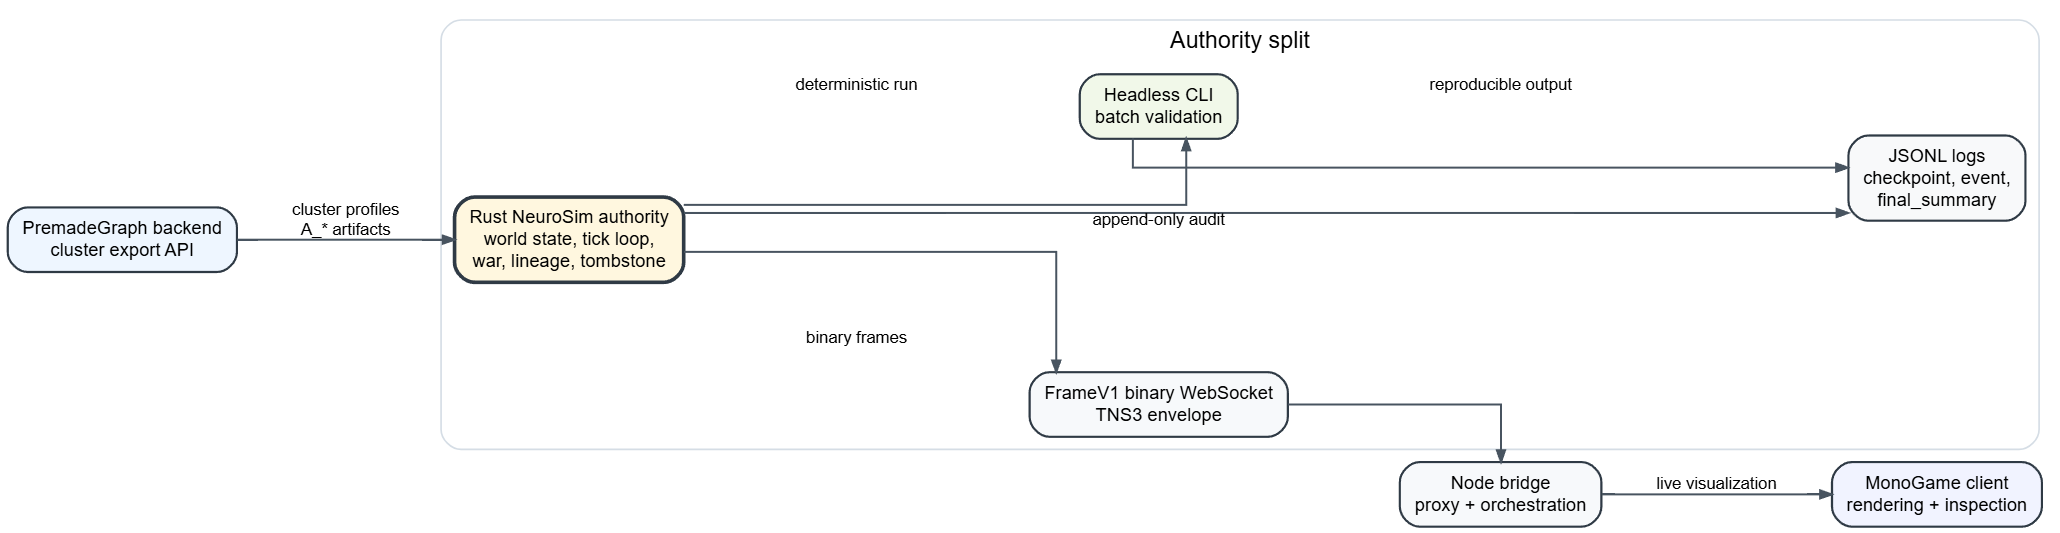
\includegraphics[width=0.92\textwidth]{assets/diagrams/thesis_neurosim_architecture_graphviz.png}
\caption{A Tribal NeuroSim hatáskör-megosztása: a Rust motor az autoritatív szimulációs állapot forrása, míg a Node és MonoGame rétegek közvetítő és megjelenítő szerepet kapnak.}
\label{fig:neurosim-architecture-graphviz}
\end{figure}

E felosztást a böngészőalapú v2 prototípus közvetlen tanulsága motiválta:
ahol a szimulációs állapot az UI-réteghez volt csatolva, ghost war jelenség,
memóriaszivárgás és nem-determinisztikus viselkedés keletkezett.
Az authority split strukturálisan kizárja e hibaosztályokat, mert a végeredmény
egyetlen Rust folyamat belső állapotától függ, nem UI-oldali értelmezéstől.

\subsection*{FrameV1 bináris protokoll}

A Rust szerver és a MonoGame kliens bináris WebSocket kereteken kommunikál.
A protokollt a TaskR7 Rust-oldali implementációja definiálta, a TaskM1 C\# dekóder
implementálta.

Minden keret egy 40 bájtos \texttt{TNS3} envelope-pal kezdődik (little-endian):

\begin{table}[h]
\centering
\caption{FrameV1 desktop envelope fejléc.}
\label{tab:framev1-envelope}
\begin{tabular}{rll}
\hline
\textbf{Offset} & \textbf{Méret} & \textbf{Mező} \\
\hline
0  & 4 B & Magic: \texttt{"TNS3"} \\
4  & 2 B & Version: \texttt{1} \\
6  & 2 B & HeaderBytes: \texttt{40} \\
8  & 2 B & PayloadKind: \texttt{2} (\texttt{FrameV1}) \\
10 & 2 B & Flags \\
12 & 4 B & PayloadBytes \\
16 & 8 B & Tick (\texttt{u64}) \\
24 & 4 B & Generation (\texttt{u32}) \\
28 & 4 B & RecordCount (élő törzsek száma) \\
32+ & változó & V1 payload \\
\hline
\end{tabular}
\end{table}

A payload section-alapú és önleíró: per-törzs rekordok (50 bájt/törzs)
után opcionálisan tile-rekordok (\texttt{FLAG\_TILE\_DATA = 0x01}, 9 bájt/tile),
háborús rekordok (\texttt{FLAG\_WAR\_DATA = 0x02}, 21 bájt/háború),
és esemény-deltók (\texttt{FLAG\_EVENT\_DATA = 0x04}) következnek.
A tile-rekordok csak elfoglalt vagy vitatott tile-okra szűkülnek,
így a hasznos terhelés arányos az aktuális aktivitással, nem a teljes térképmérettel.

A bináris formátum döntése teljesítményi és architekturális: JSON sorosítás esetén
a szimulációs tick-ciklus átbocsátóképessége összekapcsolódna a UI renderelési
ciklusával. Little-endian bináris frameknél a Rust szerver 40~ms alatt
lekezel 599 törzs állapotát, miközben a MonoGame kliens aszinkron dekódol és renderel.

Miért hatékony ez a megközelítés? Három okból. Először: a JSON sorosítás elkerülése.
Egy 599-törzsös világ JSON-alapú frissítése tick-enként ~150--200~kB felesleges szöveges
overhead-et generálna; a bináris FrameV1 ugyanezt 50~bájt/törzs + 9~bájt/aktív tile
formátumban kezeli. Másodszor: szekció-szelektivitás. A tile-rekordok csak elfoglalt
vagy vitatott tile-okra szűkülnek (\texttt{FLAG\_TILE\_DATA = 0x01}), így a payload
arányos az aktivitással, nem a teljes térképmérettel. Harmadszor: szimulációs és
UI-ciklus szétválasztása. A Rust szerver 40~ms alatt lekezel egy teljes 599-törzsös
tick-et; a MonoGame kliens aszinkron dekódol és renderel, anélkül hogy blokkolná a
szimulációs ciklust. A két folyamat egymástól függetlenül fut --- ez az architektúra
alapja annak, hogy a szimuláció egyenletesen fut magas törzsszámnál is.

\subsection*{Teljesítményproblémák és megoldásuk}

A 599-klaszteres világ bevezetésekor négy teljesítményszűkületet azonosítottunk.

A legsúlyosabb hotspot az összes-pár szomszédossági keresés volt.
A korai kód minden törzsnél az összes többi törzs összes tile-ját pásztázta végig:

\begin{lstlisting}[language={},basicstyle=\ttfamily\scriptsize,breaklines=true,caption={Régi all-pairs tile-scan: O(n\textsuperscript{2} × tiles) bottleneck}]
let my_tiles = self.tribes[i].territory.iter().copied().collect::<HashSet<_>>();
for other in &self.tribes {
    for tile in &other.territory {
        if self.world.adjacent_tiles(*tile as usize)
            .iter()
            .any(|a| my_tiles.contains(&(*a as u16))) {
            // neighboring tribe found
        }
    }
}
\end{lstlisting}

599 törzsnél ez O($n^2 \times \text{tiles}$) keresést jelentett minden 20-tickes kötegben.
A megoldás két gyorsítótár bevezetése volt:
\texttt{tile\_tribe\_idx} (\texttt{Vec<u32>}: tile~→~tulajdonos törzs indexe, O(1) lookup)
és \texttt{tribe\_id\_to\_idx} (\texttt{HashMap<u32, usize>}: törzs id~→~tömb-index, O(1)).
A gyorsítótár tick elején újraépül: ~36\,100 + 599 ≈ 36\,700 egyszerű értékadás,
amelyek után a szomszéddetektálás O($\text{my\_tiles} \times 4$) keresi a szomszédos
tulajdonost.

A vitás tile-ok nyilvántartójában O($n$) lineáris keresést szintén az O(1)
\texttt{tribe\_id\_to\_idx} cache váltotta ki.
A hot-path naplózást - 599 törzsnél tickenként százas nagyságrendű \texttt{println!}
hívás - a \texttt{headless} flag gátolja le; I/O csak checkpoint- és eseménybejegyzéseknél
keletkezik.

\subsection*{Determinizmus-hiba és javítása}

A megfigyelhetőségi igény mellé szimmetrikus követelményként társul a reprodukálhatóság:
azonos seedből azonos kimenetnek kell következnie. Ez v3 fejlesztés során
egy látens hiba miatt nem teljesült.

\textbf{A hiba:} azonos seed egymást követő MonoGame futtatások között különböző
győztest produkált.

\textbf{Gyökérok:} a \texttt{set\_clusters()} metódus rendezés nélkül fogadta
a klaszterlistát. A mögöttes SQLite-lekérdezés \texttt{ORDER BY} záradék hiányában
tetszőleges sorrendben adta vissza a sorokat, így a törzsek hex-rácsra való
elhelyezési sorrendje futtatásról futtatásra változott.
A szimuláció tick=0-ban divergált - egyetlen neurális döntés megszületése előtt.

\textbf{Javítás:} egyetlen sor a \texttt{set\_clusters()} metódusban,
a szimuláció inicializálása előtt:

\begin{lstlisting}[language={},caption={Determinizmus-javítás: klaszterek rendezése azonosító szerint}]
clusters.sort_by(|a, b| a.id.cmp(&b.id));
\end{lstlisting}

\textbf{Igazolás:} CLI mód (fejnélküli, seed=7777) és Docker-en futó MonoGame kliens
(seed=7777) tick=100-nál azonos kimenetet produkált:

\begin{lstlisting}[language={},caption={Determinizmus-ellenőrzés: CLI és MonoGame egyező eredménye tick=100-nál}]
alive=593 | City:41 | Tribe:552
\end{lstlisting}

A reprodukálhatóság a kísérleti eredmények tudományos értékének alapfeltétele:
csak olyan megfigyelés értelmezhető a modell viselkedéseként, amely azonos
körülmények között megismételhető.

\subsection*{Fejnélküli CLI mód}

A rendszer \texttt{--cli-run} flag-gel fejnélküli módban futtatható:
nincs HTTP szerver, nincs WebSocket stream, a szimuláció szinkron fut
a végkimenetelig. Ez a mód a batch-validáció és az automatizált reprodukálhatóság-ellenőrzés
elsődleges eszköze.

Kimenet: \texttt{logs/neurosim-\{seed\}-\{dataset\}-\{nonce\}.jsonl}.
Három bejegyzéstípus váltakozik: checkpoint rekordok konfigurált tick-intervallumonként,
háborús eseménybejegyzések minden deklarációra és kimenetelre,
és egyetlen \texttt{final\_summary} sor a futtatás végén.
A \texttt{final\_summary} tartalmazza a győztes azonosítóját, genomprofilját,
viselkedési archetípusát, a teljes háborús mérleget és a tombstone-összesítőt.

Öt párhuzamos fejnélküli futtatás azonos seeddel azonos \texttt{final\_summary}
győztes rekordot kell produkáljon. Ez az egyezés mérhető és automatikusan ellenőrizhető,
és erősebb bizonyíték, mint egy önmagában álló végjáték-screenshot.

A CLI futtatások teljes argumentumkészlete:
\begin{lstlisting}[language={},caption={CLI argumentumok és hatásuk}]
--cli-run            Fejnelkuli mod: nincs HTTP/WebSocket, szinkron futtas vegkimenetelig
--seed <u64>         Determinisztikus seed (pl. 42 vagy 7777)
--use-dataset-export Klaszterprofil betoltese a PremadeGraph backendbol
--require-dataset-export  Megszakitja a futtatast ha a backend nem elerheto
--ticks <u64>        Maximalis tick szam (alapertelmezs: 100000)
--checkpoint-interval <u32>  Checkpoint rekord irasanak gyakorisaga (tick)
--clusters <u32>     Szintetikus klaszterek szama (--use-dataset-export nelkul)
\end{lstlisting}

A \texttt{--require-dataset-export} flag biztosítja, hogy a batch validáció
soha ne fusson szintetikus adattal ha az a szándék valódi klaszterprofilok használata.
A \texttt{--checkpoint-interval 500} érték 599 törzsnél körülbelül 5--7 bejegyzést
ír minden checkpoint-alkalomnál, ami az I/O overhead és az elemezhetőség optimális
kompromisszuma volt a hosszú futtatásoknál.

\section{Build folyamat és telepítés}
\label{sec:neurosim-24-build}

A Tribal NeuroSim futtatási útvonala három rétegre bontható: adatexport,
Rust szimuláció és opcionális vizualizáció. A thesis szempontjából az első kettő
a lényeges, mert ezek adják a reprodukálható JSONL naplókat.

\begin{table}[h]
\centering
\caption{NeuroSim futtatási munkafolyamat.}
\label{tab:neurosim-build-flow}
\begin{tabular}{lll}
\hline
\textbf{Lépés} & \textbf{Feladat} & \textbf{Kimenet} \\
\hline
1 & PremadeGraph backend indítása & klaszterexport API \\
2 & Rust backend release fordítása & \texttt{neurosim-backend.exe} \\
3 & Fejnélküli CLI futtatás & JSONL eseménynapló \\
4 & Batch ellenőrzés & ismételhető \texttt{final\_summary} \\
5 & MonoGame kliens & élő FrameV1 vizualizáció \\
6 & Docker stack & konténeres demonstráció \\
\hline
\end{tabular}
\end{table}

A klaszterprofilokat a PremadeGraph backend szolgáltatja a
\texttt{/api/neurosim/clusters} endpointon keresztül. A Rust bináris a
\texttt{PREMADEGRAPH\_URL} és \texttt{PREMADEGRAPH\_DATASET\_ID} környezeti
változókból olvassa ki, hogy flexset vagy soloq adatkészletből inicializáljon.

\begin{lstlisting}[language={},basicstyle=\ttfamily\scriptsize,breaklines=true,caption={Egy helyre gyűjtött fejlesztői futtatási parancsok}]
# PremadeGraph backend
npm run dev

# Rust release build
cd backend/genetic-neurosim/backend
cargo build --release

# Reprodukálható CLI futás
$env:PREMADEGRAPH_URL = "http://localhost:3001"
$env:PREMADEGRAPH_DATASET_ID = "flexset"
.\target\release\neurosim-backend.exe --cli-run --seed 7777 --use-dataset-export --checkpoint-interval 500

# Batch determinizmus-ellenőrzés
.\run-batch.ps1 -Runs 5 -Seed 42 -DatasetId flexset
\end{lstlisting}

Élő vizualizáció esetén a Rust szerver FrameV1 WebSocket streamet szolgáltat,
a C\# MonoGame kliens pedig ehhez csatlakozik. Ez a mód demonstrációra alkalmas,
de a tudományos ellenőrzés alapja továbbra is a fejnélküli JSONL napló, mert abban
minden checkpoint, háborús esemény, tombstone rekord és végső összegzés
géppel visszaolvasható.

A Docker Compose konfiguráció ugyanazt a szerződést tartja meg konténeres környezetben:
a \texttt{neurosim} service csak akkor indul, ha a PremadeGraph backend healthcheck-je
sikeres, és a klaszterexport endpoint elérhető.
A seed a \texttt{NEUROSIM\_WORLD\_SEED} változóval vezérelhető;
az adatkészlet a \texttt{PREMADEGRAPH\_URL} által mutatott backend aktív datasetje lesz,
hacsak a \texttt{PREMADEGRAPH\_DATASET\_ID} expliciten meg nem adott.

\bigskip

% ===== chapters/23-tribal-neurosim-jateklogika-es-neuralis-intelligencia.tex =====
\chapter{Tribal NeuroSim - Játéklogika és Neurális Intelligencia}

\section{Neuroevolúciós keretrendszer és klaszter-alapú priorok}
\label{sec:neurosim-25-neat}

\subsection*{NEAT-stílusú neuroevolúció}

Minden szimulált törzs egy neurális hálózatot hordoz, amelynek felépítése a NEAT
(\textit{NeuroEvolution of Augmenting Topologies}) paradigmáját követi
\cite{stanleymiikkulainen2002}.
A NEAT-stílusú genomban mind a kapcsolatok súlyai, mind a hálózati topológia változhat:
új csomópontok és kapcsolatok keletkezhetnek mutáció révén, és a meglévők ki is kapcsolhatók.
A lényeges különbség a gradiens-alapú megközelítésekhez képest az, hogy a rendszer
\textit{nem alkalmaz visszaterjesztést} (backpropagation).
Nincs előre meghatározott helyes válasz, amelyhez a hálózatot igazítani kellene;
a törzs nem kap tanítójelet valós League of Legends meccssel kapcsolatban.
Ehelyett a fitnesz a szimulációs folyamat kimenetéből következik -
túlélési időből, megszerzett területből, populációméretből és elért polity-szintből -,
és minden ezer tickenként kerül kiértékelésre \cite{holland1992}.
A mutáció mértéke fitnesz szerint differenciált: a leggyengébb törzsek gyorsabban mutálnak
(kétszeres alap mutációs rátával), a legeredményesebbek konzervatívabban megőrzik genomjukat.
Az evolúciós nyomás tehát irányított, de gradiensmentes.

\begin{figure}[h]
  \centering
  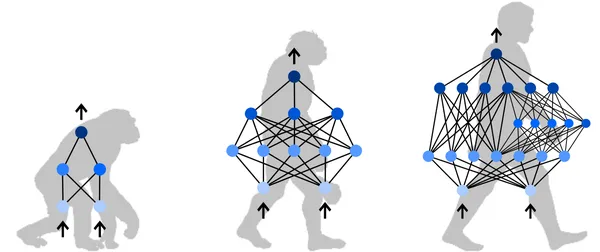
\includegraphics[width=0.74\textwidth]{assets/demo_shots/neuroevolution-mutation-ape-illustration.png}
  \caption{NEAT-stílusú neuroevolúció szemléleti ábrája: a viselkedési hálózat
    nem tanítóadatból tanul, hanem mutációval és szelekciós nyomással változtatja
    a kapcsolatok súlyait és topológiáját.}
  \label{fig:neurosim-neat-abstraction}
\end{figure}

\subsection*{Klaszter-derivált artifact priorok mint iniciális genomszekvencia}

A Tribal NeuroSim és a PremadeGraph gráfelemzési pipeline közötti közvetlen technikai hidat
az ún. \textit{artifact priorok} alkotják.
Minden törzs inicializálásakor nem véletlen paramétereket, hanem valódi meccselőzményekből
levezetett klaszterszintű teljesítménymutatókat kap inicális genomszekvenciaként:

\begin{itemize}
  \item \textbf{A\_combat} - a klaszter átlagos harci teljesítmény-pontszáma
    (ld. az OpScore metrika számítási módszertanát a 9.~fejezetben)
  \item \textbf{A\_resource} - erőforrás- és gazdaságkezelési pontszám
  \item \textbf{A\_map\_objective} - objektívkontroll-pontszám
  \item \textbf{A\_risk} - kockázattűrési pontszám
  \item \textbf{A\_team} - csapatkoordinációs pontszám
\end{itemize}

Ezek az értékek a 10.~fejezetben bemutatott klaszterezési eljárásból erednek,
és lineáris normalizációval (\(v / 10{,}0\)) kerülnek a \([0,\,1]\) tartományba.
Az inicializálás során minden törzshöz egy \texttt{Genome::new(11,~7)} struktúra jön létre -
11~bemeneti csomóponttal, 7~kimeneti csomóponttal és 84~kezdeti kapcsolattal -,
amelynek súlyait a klaszterstatisztikák befolyásolják.
A Flexset és a SoloQ adatkészletek eltérő klaszterstatisztikái eltérő iniciális genomokat
produkálnak: ez az oka annak, hogy azonos szimulációs szabályok mellett a két adatkészletből
induló törzsek eltérő viselkedési archetípusokat fejlesztenek ki (ld. a 20.~fejezet
empirikus összehasonlítását és a 24.~fejezet futtatási narratíváit).

\begin{figure}[h]
  \centering
  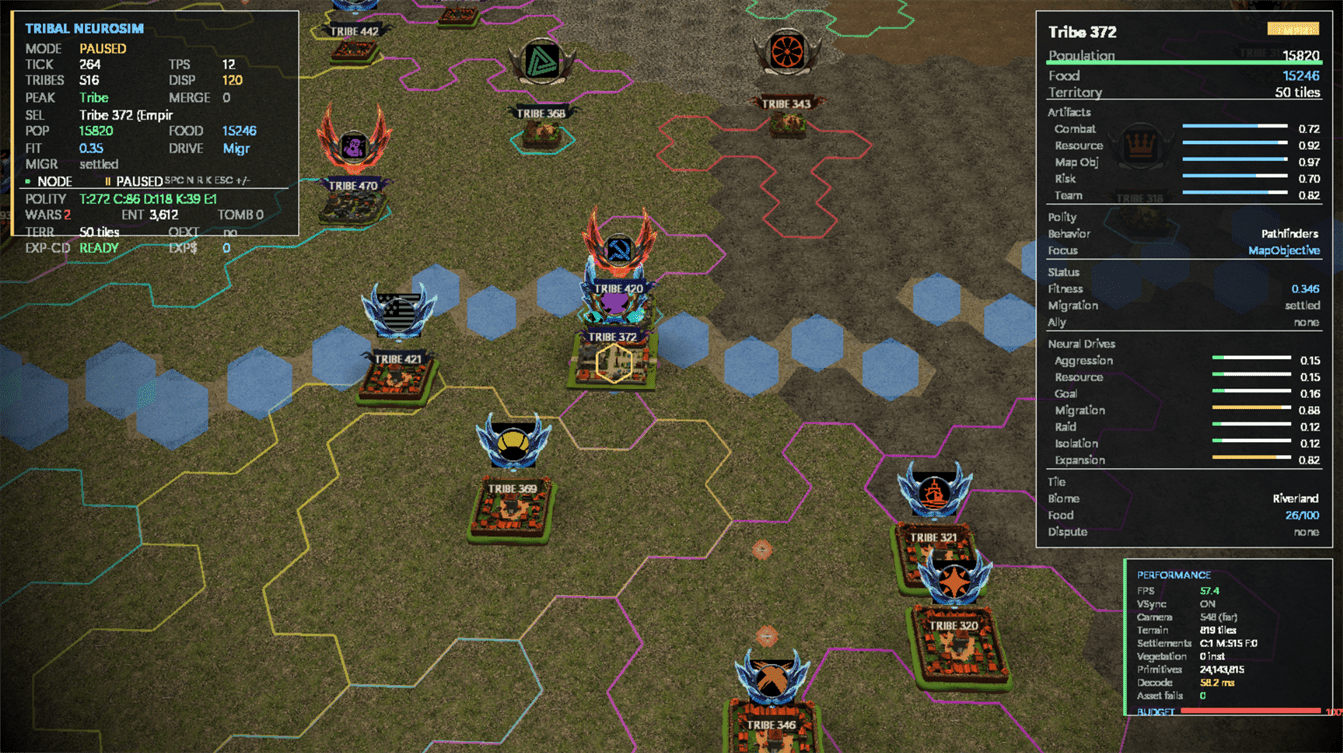
\includegraphics[width=0.9\textwidth]{assets/neurosim/run67fl7777-fl-s7777-tick264-firstempire.png}
  \caption{Flexset, seed=7777, tick=264: az első birodalom (Tribe~372, Pathfinders/MapObjective
    archetípus). A jobb oldali panelen látható artifact-sávok
    (Combat~0{,}72, Resource~0{,}92, MapObj~0{,}97)
    a klaszter-derivált iniciális priorokat tükrözik.}
  \label{fig:neurosim-fl7777-firstempire}
\end{figure}

\begin{figure}[h]
  \centering
  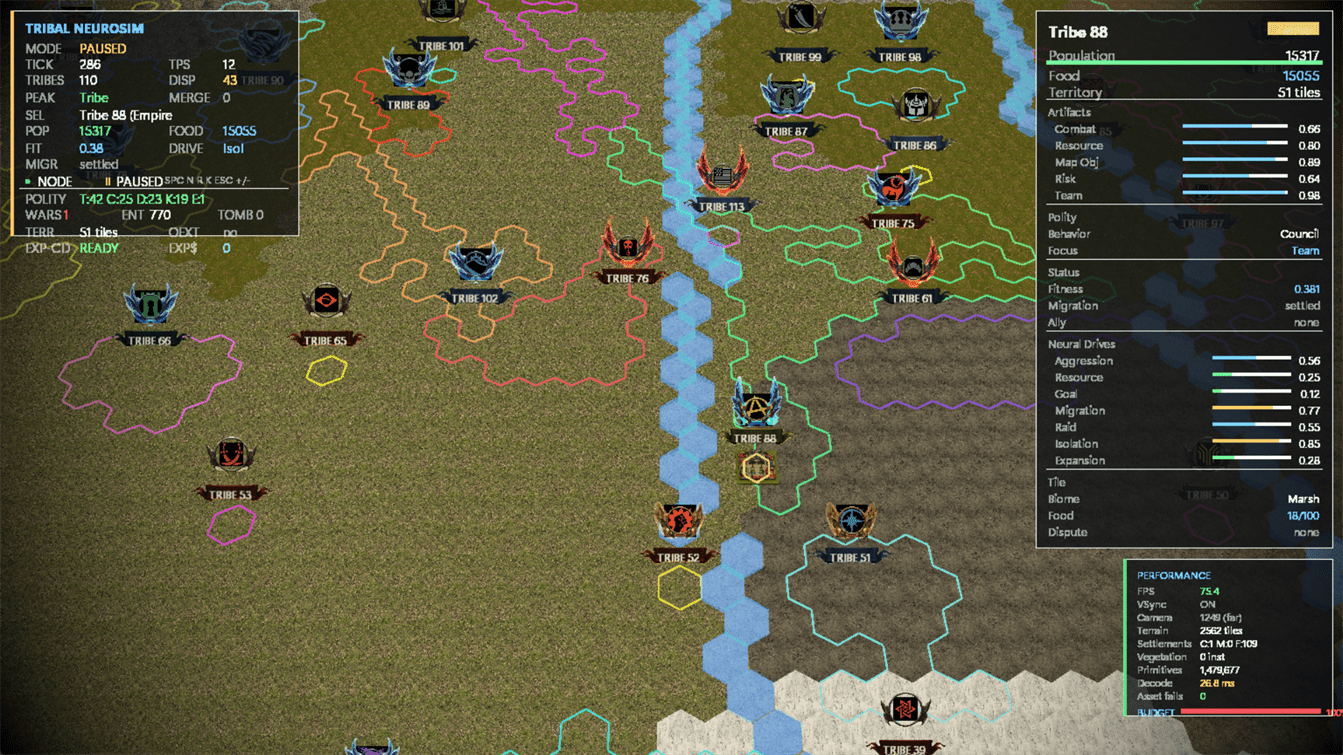
\includegraphics[width=0.9\textwidth]{assets/neurosim/run67sq42-sq-s42-tick286-firstempire.png}
  \caption{SoloQ, seed=42, tick=286: az első birodalom (Tribe~88, Council/Team archetípus).
    A Team artifact dominanciája (0{,}98) eltérő klaszterstruktúrát tükröz,
    azonos seed mellett a flexset futtatással összevetve.}
  \label{fig:neurosim-sq42-firstempire}
\end{figure}

\subsection*{Miért nem backpropagation}

A neurális hálózat nem prediktív modell és nem osztályozó - \textit{személyiség- és
hajtóerő-generátor}. Hét kimeneti értéke (\textit{aggression}, \textit{resource\_drive},
\textit{goal\_drive}, \textit{migration\_drive}, \textit{raid\_drive}, \textit{isolation},
\textit{expansion\_speed}) valószínűségi küszöböket modulál egy determinisztikus
állapotgépben; nem bináris döntések, hanem folytonos torzítások.
Ehhez nincs szükség labeled training célra: a törzs nem tanulja meg, mi az \textit{helyes}
viselkedés egy adott meccspillanatban, hanem a szimulációs versenynyomás alatt adaptálódik
a saját klaszterprofilból induló genomjával.
Ha a törzs genomiálisan agresszív, a háborúindítási küszöb könnyebben teljesül;
ha a migráció-hajtóerő magas, a törzs áttelepül, amikor még \textit{Settling} állapotban van.
A fitnesz ebből következik, nem fordítva.

\subsection*{Genomcache és teljesítményszempont}

A fordított (\textit{compiled}) genomcache tick-ek között újrafelhasználódik:
a \texttt{genome.compile()} hívás egy \texttt{CompiledGenome}-ot állít elő,
amely a topológiai előre-átmeneti lépéstervet tárolja.
A \texttt{CompiledGenome::activate(\&inputs[0..11])} meghívása minden tickben elvégzi
a neurális inferenciát anélkül, hogy a hálózatot újraépítené.
A cache csak mutációkor (minden ezer tickenként, generációs határponton)
és polity-fúziókor (\texttt{Genome::inherit\_from()} hívásakor) érvénytelenítődik,
amikor a két törzs genomjából fitnesz-súlyozott keveréssel keletkezik az örökös genomja.

A következő szekcióban a konkrét bemenet-kimenet architektúrát és a 11~bemeneti jel
részletes leképezését tárgyaljuk.

% ============================================================
\section{Neurális bemenetek, hajtóerők és viselkedési kimenetek}
\label{sec:neurosim-25-drives}

A 23.1~szekcióban ismertetett NEAT-stílusú genomból minden tickben egy konkrét
11~bemeneti jelre épülő következtetés indul el, amelynek eredménye 7~kimeneti hajtóerő.
Ez a bem\-enet-kimenet architektúra adja a neurális réteg és a determinisztikus
állapotgép közötti határfelületet: a hálózat nem parancsokat ad ki, hanem folytonos
torzításokat, amelyek a törzs következő döntéseinek valószínűségi eloszlását alakítják.

\subsection*{A 11 bemeneti jel}

A \texttt{CompiledGenome::activate()} hívás 11~értékből álló vektort kap.
Az első négy dinamikus: értékük tickenként változik a szimulált világ aktuális
állapotától függően. A következő öt invariáns: a klaszter-derivált artifact priorokból
jönnek létre inicializáláskor, és csak generációs határpontokon (minden 1000.~ticknél)
frissülnek, mutáció eredményeként. Az utolsó két bemeneti jel szintén dinamikus,
és a törzs térbeli elhelyezkedéséből következik.

\begin{table}[h]
  \centering
  \caption{A neurális hálózat 11 bemeneti jele.}
  \label{tab:neurosim-inputs}
  \begin{tabular}{clll}
    \hline
    \textbf{Index} & \textbf{Változónév} & \textbf{Leírás} & \textbf{Jelleg} \\
    \hline
    0 & \texttt{food\_ratio}         & Élelmiszerkészlet / populáció         & Dinamikus \\
    1 & \texttt{pop\_ratio}          & Populáció / maximális kapacitás        & Dinamikus \\
    2 & \texttt{territory}           & Igényelt tile-ok száma / 100           & Dinamikus \\
    3 & \texttt{feed\_risk}          & Éhhalál-közelség (1{,}0 = kritikus)   & Dinamikus \\
    4 & \texttt{a\_combat}           & Harci teljesítmény-artifact             & Invariáns* \\
    5 & \texttt{a\_resource}         & Erőforrás/gazdaság-artifact             & Invariáns* \\
    6 & \texttt{a\_map\_objective}   & Objektívkontroll-artifact               & Invariáns* \\
    7 & \texttt{a\_team}             & Csapatkoordinációs artifact             & Invariáns* \\
    8 & \texttt{nearest\_enemy}      & Legközelebbi ellenfél hex-távolsága    & Dinamikus \\
    9 & \texttt{nearest\_ally}       & Legközelebbi szövetséges hex-távolsága & Dinamikus \\
   10 & \texttt{a\_risk}             & Kockázattűrési artifact                 & Invariáns* \\
    \hline
  \end{tabular}
  \begin{flushleft}
    \small{* Csak generációs határpontokon (1000 tickenként) frissül, mutáció révén.}
  \end{flushleft}
\end{table}

A \texttt{nearest\_enemy} és \texttt{nearest\_ally} jelek \([0,\,1]\) tartományba
normalizált hex-távolságok; értékük~1{,}0, ha nincs elérhető ellenfél, illetve szövetséges.
Ezzel a két jel a törzs térbeli elszigeteltségét kódolja: a közelben lévő ellenség
alacsony értéket, a magányos elhelyezkedés magas értéket jelent.

\begin{figure}[h]
\centering
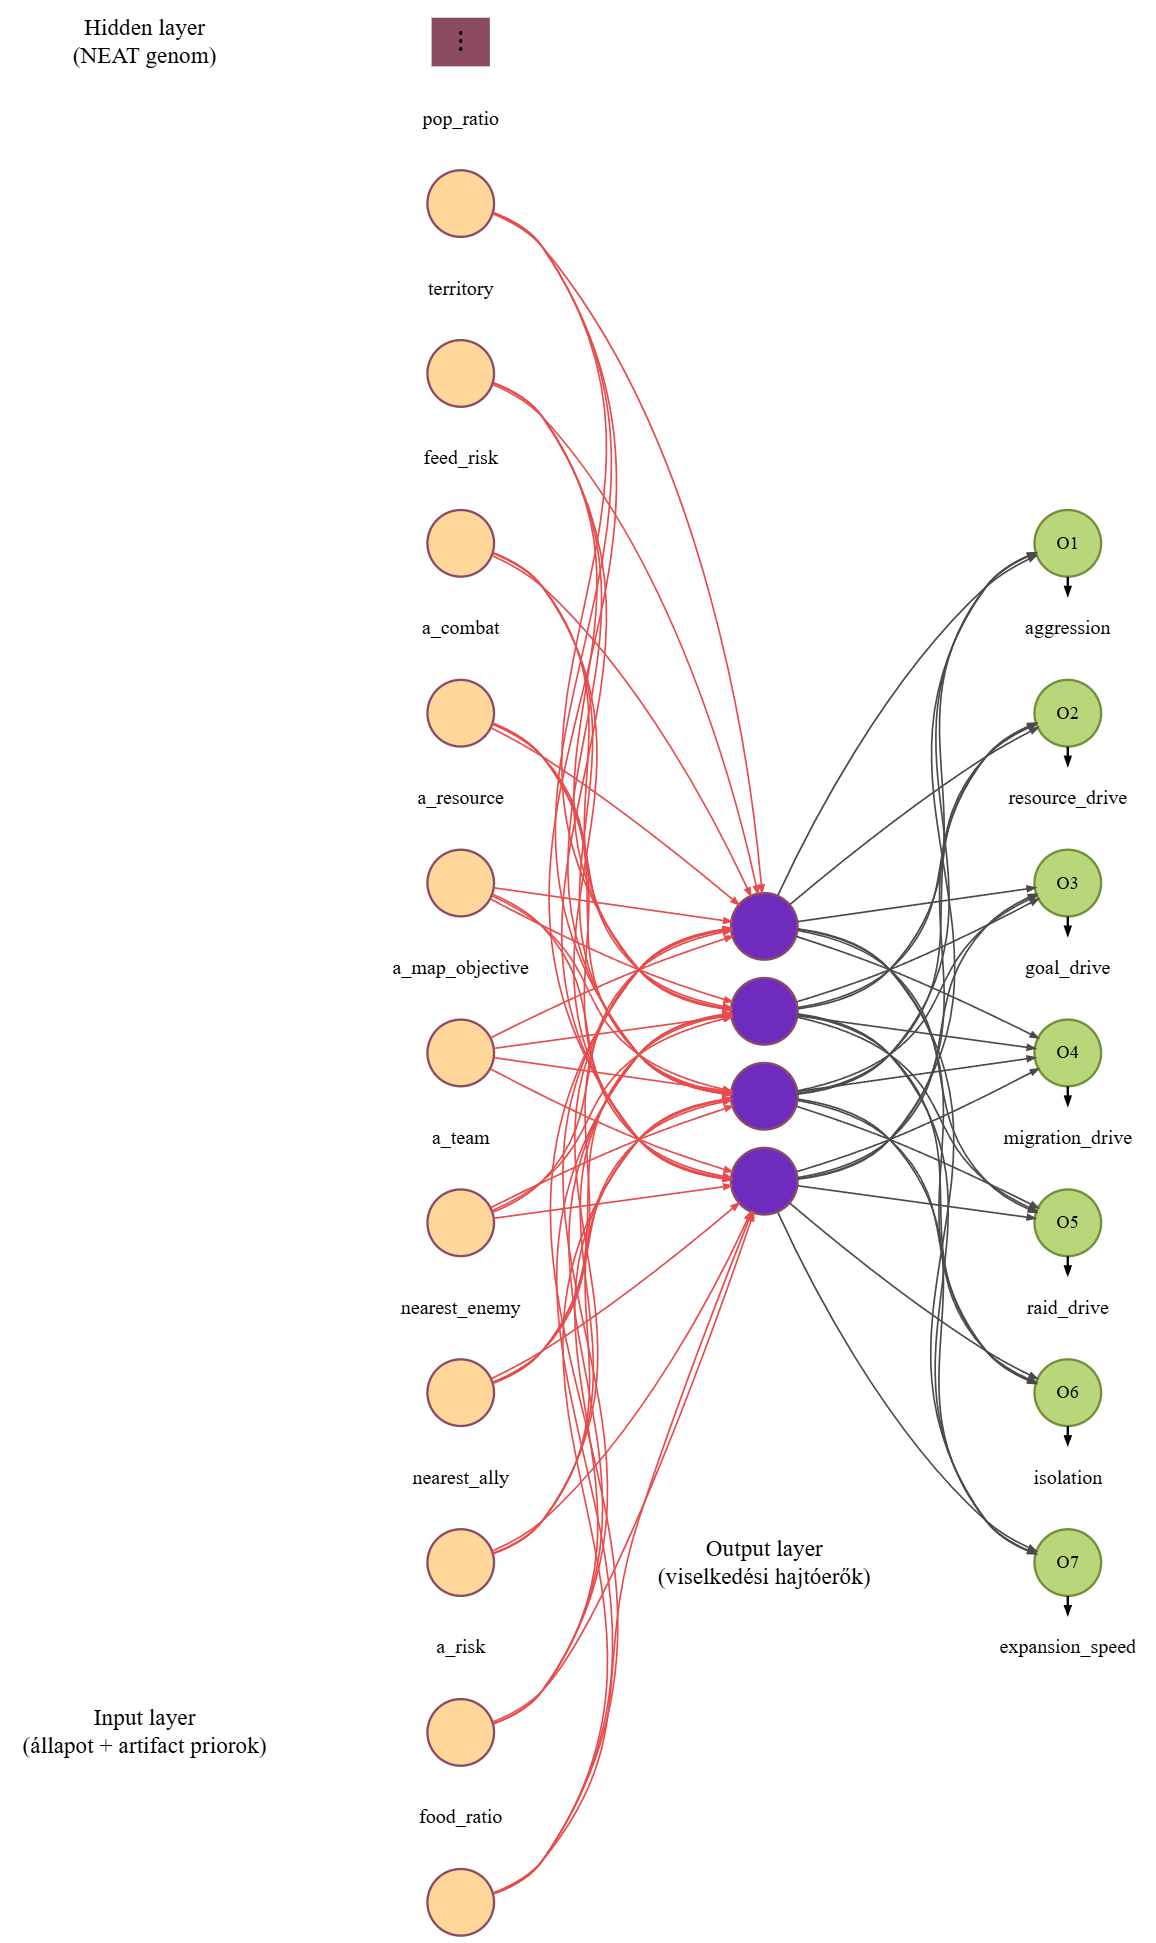
\includegraphics[width=0.75\textwidth]{assets/diagrams/genome_graph.png}
\caption{A Tribal NeuroSim genomjának réteges értelmezése: a 11 bemeneti jel a NEAT-stílusú genomon keresztül 7 viselkedési hajtóerőt állít elő.}
\label{fig:neurosim-genome-graph}
\end{figure}

\subsection*{A 7 kimeneti hajtóerő}

A hálózat kimenete \texttt{tanh} aktivációs függvényen keresztül keletkezik,
így minden érték a \([-1,\,1]\) tartományba esik.
A kimenetek az állapotgép küszöbértékeit modulálják; az állapotgép a küszöböket
determinisztikusan ellenőrzi, de a küszöbök teljesülési valószínűsége a hajtóerőktől függ.

\begin{table}[h]
  \centering
  \caption{A 7 kimeneti hajtóerő és hatásuk a törzs viselkedésére.}
  \label{tab:neurosim-outputs}
  \begin{tabular}{lll}
    \hline
    \textbf{Változónév} & \textbf{Viselkedési hatás} & \textbf{Aktiválási küszöb} \\
    \hline
    \texttt{aggression}      & Háborúindítási valószínűség modulálása       & $> 0{,}45$ \\
    \texttt{resource\_drive} & Területterjeszkedési prioritás                & $> 0{,}25$ \\
    \texttt{goal\_drive}     & Szövetségkezdeményezés, polity-fejlesztés     & $> 0{,}55$ / $> 0{,}50$ \\
    \texttt{migration\_drive}& Migráció indítása (\textit{Settling} állapotból) & $> 0{,}55$ \\
    \texttt{raid\_drive}     & Opportunista háború gyengébb szomszéd ellen  & $> 0{,}35$ \\
    \texttt{isolation}       & Szövetségajánlat elutasítása                 & $> 0{,}75$ \\
    \texttt{expansion\_speed}& Tile-igénylési sebesség (hűtési idő módosítás) & Folytonos \\
    \hline
  \end{tabular}
\end{table}

\subsection*{Hogyan válnak a kimenetek viselkedéssé}

A hajtóerők nem bináris kapcsolók - \textit{folytonos valószínűségi modulátorok}.
Az állapotgép a hajtóerők értékeit küszöbökkel veti össze, de a küszöbök teljesülése
nem szükségszerűen vált ki azonnal állapotátmenetet: az adott viselkedési ág
egyéb feltételektől (szomszéd jelenléte, élelmiszertartalék, ticks\_in\_state)
is függ. Három jellemző összefüggés:

\begin{itemize}
  \item \textbf{Opportunista háború:} \texttt{raid\_drive}~$> 0{,}35$ \textit{és}
    \texttt{food\_ratio}~$> 0{,}5$ \textit{és} gyengébb szomszéd létezik
    $\Rightarrow$ \texttt{AtWar} állapotátmenet, céltörzs = leggyengébb
    szomszéd (\texttt{pop~$\times$~a\_combat} alapján).
  \item \textbf{Migráció:} \texttt{migration\_drive}~$> 0{,}55$ \textit{és}
    legalább 15~tick eltelt \texttt{Settling} állapotban
    $\Rightarrow$ célpont kiválasztása (\texttt{pick\_migration\_dest}),
    majd lépésenként hexagonális elmozdulás.
  \item \textbf{Szövetség-blokkolás:} \texttt{isolation}~$> 0{,}75$
    $\Rightarrow$ a szövetségajánlat elutasítódik, még akkor is, ha
    \texttt{goal\_drive} egyébként szövetséget indítana.
\end{itemize}

Az \texttt{expansion\_speed} kimenet közvetlen numerikus módosító: a tile-igénylés
hűtési idejét (\textit{expansion cooldown}) arányosan csökkenti, így a magas értékű
törzsek gyorsabban terjeszkednek azonos élelmiszertartalék és populáció mellett.

\subsection*{A küszöbértékek indoklása}

A \ref{tab:neurosim-outputs}.~táblázatban szereplő aktiválási küszöbök nem önkényesek, hanem
a liveness-fix utáni iteratív kalibrálás eredményei.

\textbf{raid\_drive küszöb (0{,}35):} Alacsonyabb értéknél (pl. 0{,}20) szinte
minden törzs folyamatosan opportunista háborút indít, függetlenül a valódi
erőforrás-helyzettől --- ez a korai futtatások ,,overaggression'' hibájának
reprodukciója. Magasabb értéknél (pl. 0{,}55) a legtöbb törzs soha nem indít
opportunista háborút, és a szimuláció stagnálásba kerül.

\textbf{isolation küszöb (0{,}75):} Alacsonyabb értéknél a szövetségesek száma
exponenciálisan nő, és a szimuláció lassú, kooperatív blokkképzéssé válik
ahelyett, hogy versengő konszolidáció zajlana. Magasabb értéknél minden törzs
izolálódik, és a fuzionálás soha nem következik be, ami kizárja a genomiális
sokszínűség terjedését.

\textbf{migration\_drive küszöb (0{,}55):} Ez volt a legkritikusabb kalibráció.
A post-first-run diagnózis kimutatta, hogy 0{,}45-ös küszöbnél a törzsek 90\%-a
folyamatos migrációs oszcillációba kerül; 0{,}65 felett a migráció szinte soha
nem indul el, és a területi lefedettség alacsony marad. A 0{,}55-ös érték
az a pont, ahol a törzs csak akkor vándorol, ha a migrációs igény
szignifikánsan meghaladja az alapzajt.

\subsection*{F2 korai futtatás: kimeneti aktivitás ellenőrzése}

Az F2 futtatás (Flexset adatkészlet, 599~törzs, 1200~tick) korai mérési pontként
rögzítette az összes törzs neurális aktivációját. A szerepe itt nem az, hogy a
végleges verziót bizonyítsa, hanem az, hogy megmutassa: a hét kimeneti hajtóerő
nem maradt inaktív, és a hálózat képes volt különböző viselkedési torzításokat adni
a törzsek állapotgépének (\ref{tab:neurosim-f2-outputs}.~táblázat).

\begin{table}[h]
  \centering
  \caption{A 7 kimeneti hajtóerő dominancia-megoszlása az F2 korai futtatásban
    (1200~tick, 599~törzs, Flexset adatkészlet).}
  \label{tab:neurosim-f2-outputs}
  \begin{tabular}{lrr}
    \hline
    \textbf{Kimeneti hajtóerő} & \textbf{Domináns aktiváció (db)} & \textbf{Arány} \\
    \hline
    \texttt{migration\_drive} & 6\,526 & 38{,}4\% \\
    \texttt{goal\_drive}      & 3\,127 & 18{,}4\% \\
    \texttt{expansion\_speed} & 3\,060 & 18{,}0\% \\
    \texttt{isolation}        & 1\,823 & 10{,}7\% \\
    \texttt{resource\_drive}  & 1\,546 &  9{,}1\% \\
    \texttt{raid\_drive}      &   634 &  3{,}7\% \\
    \texttt{aggression}       &   258 &  1{,}5\% \\
    \hline
    \textbf{Összesen}         & 16\,974 & 100\% \\
    \hline
  \end{tabular}
\end{table}

Az aktivitásmegoszlás minden 100~tickes ablakban stabil maradt: a tick~0-99,
400-499, 800-899 és 1100-1200 intervallumokban mind a 7~kimenet jelen volt.
A kimeneti erősség tartománya 0{,}221-től 0{,}881-ig terjedt (terjedelem: 0{,}660),
ami telítetlen, valóban differenciált aktivitásra utal.
Az átlagos fitnesz tick=1-en 0{,}008 volt; tick=1200-ra 0{,}277-re emelkedett,
és az átlag-maximum különbség (0{,}003-ról 0{,}279-re nőtt) arra utalt,
hogy a fitnesz-függvény már ebben a korai állapotban is elkezdte szétválasztani
a törzseket. A későbbi futások értelmezéséhez azonban a javított, determinisztikus
logokra kell támaszkodni, nem erre az F2-es mérésre.

Az \texttt{aggression} hajtóerő alacsony részesedése (1{,}5\%) nem hibajelzés:
a direkt agressziót a \texttt{raid\_drive} és a \texttt{goal\_drive} egyaránt
átfedik, más aktiválási feltétellel. A migráció dominanciája (38{,}4\%) pedig
összhangban van a flexset klaszterprofilok magas \texttt{A\_map\_objective}
értékeivel, amelyek a térhasználatot és mozgást ösztönzik.

\begin{figure}[h]
  \centering
  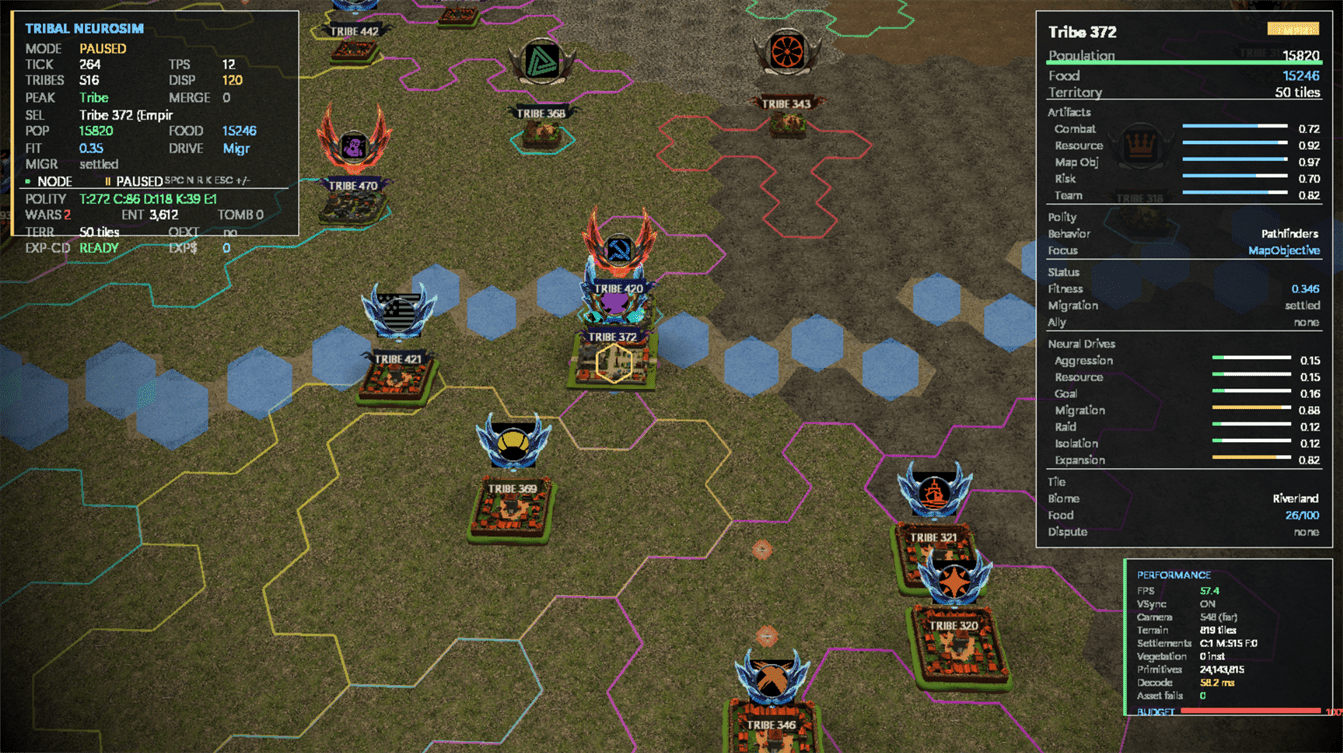
\includegraphics[width=0.9\textwidth]{assets/neurosim/run67fl7777-fl-s7777-tick264-firstempire.png}
  \caption{Tribe~372 jobb oldali paneljén a Neural Drives sávok (Flexset, seed=7777, tick=264):
    Migration=0{,}88 és Expansion=0{,}82 dominál, Aggression=0{,}15 minimális.
    Ez a Pathfinders/MapObjective archetípus hajtóerő-profilja.}
  \label{fig:neurosim-fl7777-drives-early}
\end{figure}

\begin{figure}[h]
  \centering
  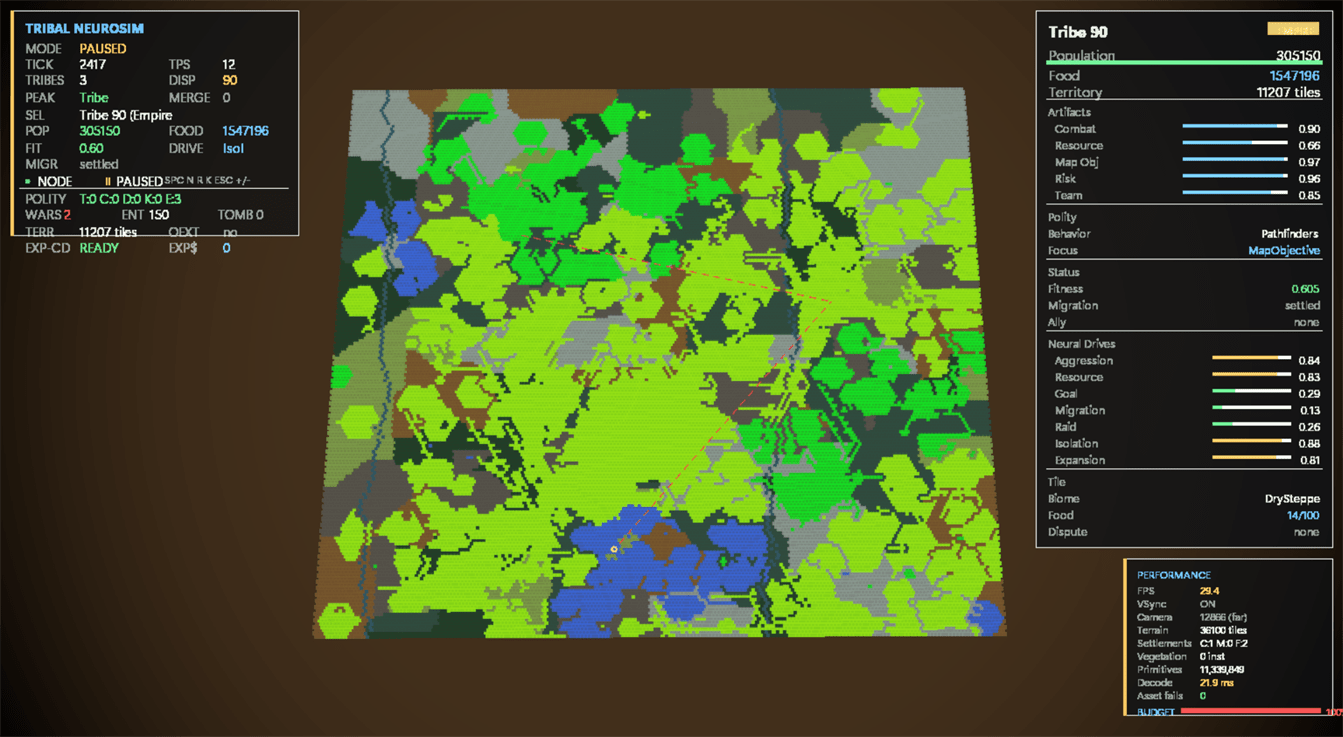
\includegraphics[width=0.9\textwidth]{assets/neurosim/run67fl42-fl-s42-tick2417-trilateralwar.png}
  \caption{Tribe~90 a trilaterális háború pillanatában (Flexset, seed=42, tick=2417):
    Aggression=0{,}84, Resource=0{,}83 - markánsan eltérő hajtóerő-profil
    ugyanolyan adatkészletből, eltérő genomevolúció eredményeként.}
  \label{fig:neurosim-fl42-trilateral-drives}
\end{figure}

\subsection*{A liveness-fix tanulsága: differenciáció, nem pusztán aktivitás}

A 2026.~május~14-i szimulációs liveness-fix előtt a futtatás látszólag élőnek tűnt -
mozgás volt, háborúk is folytak -, de fitnesz-differenciáció nem keletkezett.
A vizsgálat három egymást erősítő hibát tárt fel.

Első hiba: a törzs-statisztikák kétszeres normalizálása.
A \texttt{server.js} már \([0,\,1]\) tartományra hozta az artifact értékeket,
majd a Rust engine ismét elosztotta őket 10-zel.
Ennek eredménye: az \texttt{a\_combat} értéke a várható $\approx0{,}3$ helyett
$\approx0{,}03$ lett, így minden harci forduló mindössze $0{,}03 \times 6000 \times 0{,}02 = 3{,}6$
veszteséget okozott - a háborúk soha nem öltek meg senkit.

Második hiba: a migráció-hajtóerő oszcilláció.
A \texttt{Settling} állapotból azonnali migrációs átmenet tüzelt, ha
\texttt{migration\_drive}~$> 0{,}55$, és a törzs visszaérkezése után
ismét tüzelt. A törzsek körülbelül 15\%-a így soha nem maradt elég ideig
\texttt{Settling} állapotban ahhoz, hogy területet igényeljen.

Harmadik hiba: túl konzervatív terjeszkedési küszöb.
A \texttt{resource\_drive}~$< 0{,}25$ feltétel a törzsek $\approx63$\%-át zárta
ki a terjeszkedésből.

Mindhárom hibajavítás után a neurális kimenet \textit{mérhetően differenciált}
viselkedést produkált: az átlagos fitnesz és a legjobb törzs fitnesze között
markáns rés keletkezett, és a populációból elkülönülő győztesek emelkedtek ki.
A tanulság tehát nem csupán az, hogy mind a 7~kimenet aktív legyen,
hanem az, hogy a kimenetek \textit{mért eltéréseket} okozzanak a túlélési
esélyekben - különben a neurális réteg látható, de hatástalan marad.

% ============================================================
\section{Fitness, mutáció és leszármazási öröklés}
\label{sec:neurosim-25-fitness}

A 23.1~szekcióban ismertetett genomevolúció és a 23.2~szekcióban részletezett
hajtóerő-architektúra csak akkor hoz mérhetően eltérő kimeneteket, ha az evolúciós
nyomás - a fitnesz-függvény, a mutációs mechanizmus és az öröklési szabályok -
helyesen van kalibrálva. E szekció ezeket a mechanizmusokat tárgyalja részletesen.

\subsection*{Fitness komponensek}

A törzs fitnesz-értéke nem egyetlen összesített szám; öt komponens együttesen
befolyásolja a mutációs rátát, a fuzionálási döntést és a genomöröklés arányát.
A komponensek:

\begin{itemize}
  \item \textbf{survival\_ticks} - a törzs által eddig eltöltött tickek száma.
    Hosszabb túlélés önmagában is fitneszelőnyt jelent, hiszen a szimulált verseny
    természete szerint a kihalt törzsek nem örökítenek tovább.
  \item \textbf{territory} - az értékelés pillanatában igényelt tile-ok száma.
    Területnagyság és erőforrás-hozzáférés szorosan kötött: a kis területű törzs
    élelmiszerhiányra és populációcsökkentésre van ítélve.
  \item \textbf{population} - az aktuális populációméret. A magas populáció
    háborús ellenálló-képességet és terjeszkedési potenciált egyaránt növel.
  \item \textbf{polity\_tier} - az elért politikai szint numerikusan kódolva:
    Tribe\,=\,1, City\,=\,2, Duchy\,=\,3, Kingdom\,=\,4, Empire\,=\,5.
    A magasabb polity-szint küszöbfeltételekhez kötött (populáció, terület,
    \texttt{goal\_drive}), ezért önmagában is a koordinált stratégia jelzője.
  \item \textbf{war\_record} - a megnyert háborúk száma. Minden győzelem
    hozzáadódik a törzs harci tapasztalatához és a 23.1~szekcióban ismertetett
    \texttt{A\_combat} artifact értékéhez (ld. az artifact felhalmozódásáról szóló
    részt lejjebb).
\end{itemize}

A komponensek egymást nem helyettesítik: egy sok háborút megnyert, de kis területű
törzs eltérő genomevolúciós pályát követ, mint egy háborút soha nem vívott,
de hatalmas területet felhalmozó törzs.

\subsection*{Mutáció mechanizmusa}

A mutáció minden 1000.~ticknél - az ún. \textit{generációs határponton} - következik be.
A határponton a szimuláció fitnesz szerint rangsorolja az összes élő törzset,
és differenciált mutációs rátát alkalmaz:

\begin{itemize}
  \item \textbf{Leggyengébb 20\%}: kétszeres alap mutációs ráta - nagyobb esély
    az áttörésre, de egyúttal nagyobb esély a kontraproduktív változásokra is.
  \item \textbf{Felső 20\%}: az alap mutációs ráta fele - a sikeres stratégia
    konzervatívabban megmarad, de nem válik teljesen merevvé.
  \item \textbf{Középső 60\%}: alap mutációs ráta.
\end{itemize}

A mutáció négy típusa:
\begin{enumerate}
  \item \textbf{Súlymódosítás} - egy meglévő kapcsolat súlya kis mértékű
    ($\pm$perturbáció) változást szenved.
  \item \textbf{Kapcsolat hozzáadása} - két korábban nem összekötött csomópont
    között új él jön létre.
  \item \textbf{Kapcsolat letiltása} - egy meglévő kapcsolat inaktívvá válik
    (de a nyilvántartásban megmarad, esetleges reaktiváláshoz).
  \item \textbf{Csomópont hozzáadása} - egy meglévő él két részre osztódik
    egy közbülső csomópont beillesztésével, növelve a hálózat mélységét.
\end{enumerate}

A mutációs ráta ($\mu$) nem egyetlen konstans. Az alap érték $\mu_0 = 0{,}05$
(5\% esély súlymódosításra tickenként mutáción belül). A fitnesz-rangsor alapján
ez differenciált:

\begin{equation}
\mu_i =
\begin{cases}
2\mu_0 & \text{ha } r_i \leq 0{,}20 \text{ (leggyengébb 20\%)} \\
\mu_0  & \text{ha } 0{,}20 < r_i < 0{,}80 \\
\tfrac{1}{2}\mu_0 & \text{ha } r_i \geq 0{,}80 \text{ (felső 20\%)}
\end{cases}
\end{equation}

ahol $r_i \in [0,1]$ az $i$-edik törzs relatív fitnesz-rangszáma a populációban.
A $2\mu_0$ ráta magasabb esélyt ad az áttörésre, de egyúttal magasabb esélyt
a kontraproduktív változásokra is; a $\tfrac{1}{2}\mu_0$ ráta a sikeres genomot
konzerválja anélkül, hogy teljesen merevvé tenné.

Fontos megkülönböztetés: \textit{generációs határponton nincs crossover}
két különböző törzs genomja között. A genomkeverés kizárólag fuzionáláskor
történik, az örökös létrehozásakor.

\subsection*{Fuzionálás és fitnesz-súlyozott genomöröklés}

Két törzs fuzionálhat, ha mindkettőre teljesül: \texttt{goal\_drive}~$> 0{,}55$,
egyik sem tartózkodik \texttt{AtWar} állapotban, és mindkettőre
\texttt{isolation}~$< 0{,}75$.
Ez utóbbi feltétel közvetlen összefüggésben áll a 23.2~szekcióban ismertetett
\texttt{isolation} hajtóerővel: az erősen izolacionista genomú törzs blokkolja
a szövetségajánlatot, ezért fuzionálásra sem kerülhet sor.

A fuzionálásból keletkező örökös genomja a \texttt{Genome::inherit\_from(parent\_a,
parent\_b, fitness\_a, fitness\_b)} hívással jön létre: fitnesz-súlyozott keverék,
amelyben az erősebb szülő genomja dominálja az örökséget.
Minden tile, populáció és élelmiszerkészlet az örökös törzshöz kerül.
Az eltűnő szülő tombstone rekordot kap, amelynek okfeljegyzése \textit{fuzionálás}
- megkülönböztethető a harci vereségtől.

A genomcache a fuzionáláskor érvénytelenítődik (ld. 23.1~szekció),
így az örökös első tickjén újrafordítja a kevert genomot.

\subsection*{Leszármazási DAG és LineageRegistry}

Minden törzs nyilvántartja az \texttt{entity\_id $\to$ [parent\_ids]} leképezést.
A seed-entitásoknál - vagyis az inicializáláskor közvetlenül klaszterprofilból
létrehozott törzsek esetén - a szülő \texttt{u32::MAX} sentinel értéket kap;
ezek a leszármazási DAG gyökerei.

A TaskR1 implementációs futtatás (2026.~május~6.) vezette be a \texttt{LineageRegistry}
struktúrát:

\begin{lstlisting}[language={}, caption={A LineageRegistry kompakt adatstruktúrája.},
  label={lst:lineage-registry}]
struct LineageRegistry {
    // Key: entity_id, Value: (parent_a_id, parent_b_id)
    registry: HashMap<u32, (u32, u32)>,
    next_id: u32,
}
\end{lstlisting}

\begin{figure}[h]
\centering
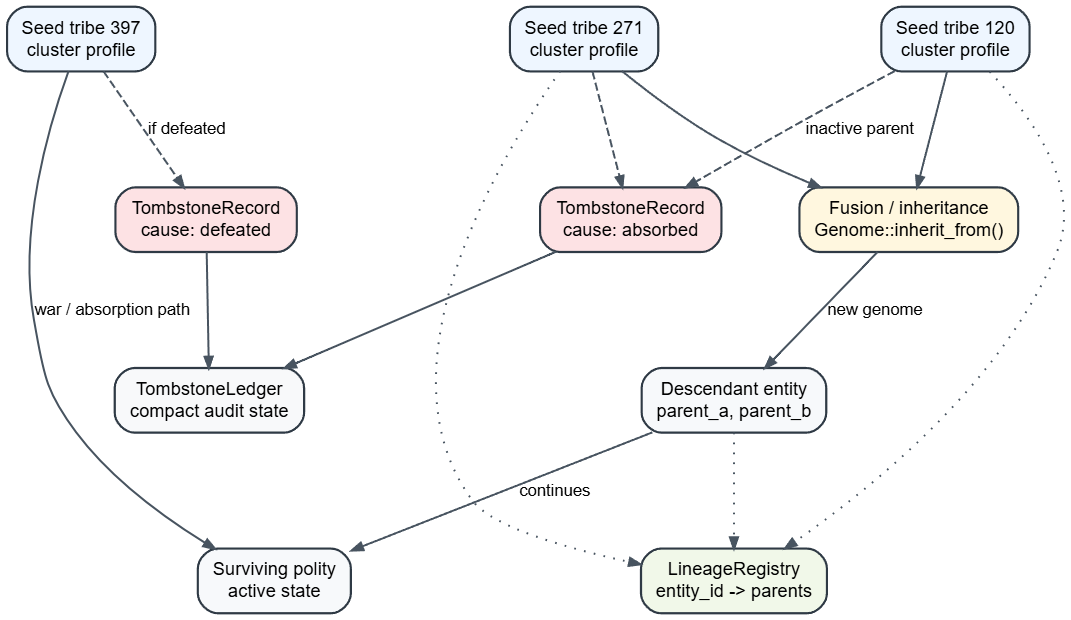
\includegraphics[width=0.92\textwidth]{assets/diagrams/thesis_lineage_tombstone_dag_graphviz.png}
\caption{A leszármazási és tombstone modell DAG-szerkezete: az aktív és kihalt törzsek auditálható szülői linkeken és kompakt rekordokon keresztül maradnak visszakövethetők.}
\label{fig:lineage-tombstone-dag}
\end{figure}

A szülői-link alapú tárolás egy irányított aciklikus gráf (DAG) szerkezetét
valósítja meg. Formálisan: legyen $V$ az összes entitás-csúcsok halmaza és
$E \subseteq V \times V$ az örökségi élek halmaza, ahol $(v_p, v_c) \in E$
azt jelenti, hogy $v_p$ szülője $v_c$-nek. A struktúra aciklikus, mert
a fuzionálásból megszülető törzs nem lehet saját ősének szülője.
Az ősfa bejárása bármely $v$-re $O(d)$ időben elvégezhető, ahol $d$ a leszármazási
mélység \cite{cormen2009}.

A kompakt szülői-link megközelítés rokon a Ziv--Lempel-féle szótárépítő elvvel
\cite{zivlempel1977}: nem az összes ős kerül tárolásra (ami a szótár méretének
exponenciális növekedésével lenne ekvivalens), hanem csak az azonnali szülők,
amelyekből a teljes lánc rekurzív lekérdezéssel felépíthető. Ez az információs
tömörítési stratégia a lineage-ek esetén azért különösen hatékony, mert
a törzspopuláció legtöbb tagja 2--4 generáción belül elérhető az azonosítójukból.

A REST endpointok:
\begin{itemize}
  \item \texttt{GET /api/lineage/resolve/\{entity\_id\}} - a szülőlánc DAG visszaadása
  \item \texttt{GET /api/lineage/seed/\{entity\_id\}} - visszakövetés az eredeti
    klaszterazonosítóig
  \item \texttt{GET /api/lineage/stats} - az összes entitás száma és
    seed-klaszter megoszlása
\end{itemize}

Postmortem lekérdezés: bármely kihalt törzs teljes leszármazási lánca visszakereshető
a tombstone rekord és a LineageRegistry kombinációján keresztül.

\subsection*{Artifact felhalmozódás mint harci tapasztalat}

Az \texttt{A\_combat} érték nem marad rögzített az inicializálás utáni szinten.
Minden megnyert háború után növekszik: a törzs tényleges harci tapasztalata
kumulálódik a genomba, fokozatosan felülírva a klaszter-derivált iniciális priort.
Ez a legfontosabb különbség az inicializálási állapot és a futtatás végi érték között:
egy alacsony \texttt{A\_combat}-tal induló törzs - ha elegendő védelmi győzelmet arat -
képes magas harci tapasztalatot felhalmozni.

A legmarkánsabb bizonyíték erre a Flexset seed=7777 futtatás győztese, Tribe~355.
A futtatás végén (tick=2538) mért \texttt{A\_combat}~$= 0{,}98$ szinte pontosan
a lehetséges maximum - holott a törzs nem különösen magas iniciális harci priorral
indult. A 2538~tick során megnyert összes védelmi háború kumulált hatása emelte az
értéket a telítési határra.

\begin{figure}[h]
  \centering
  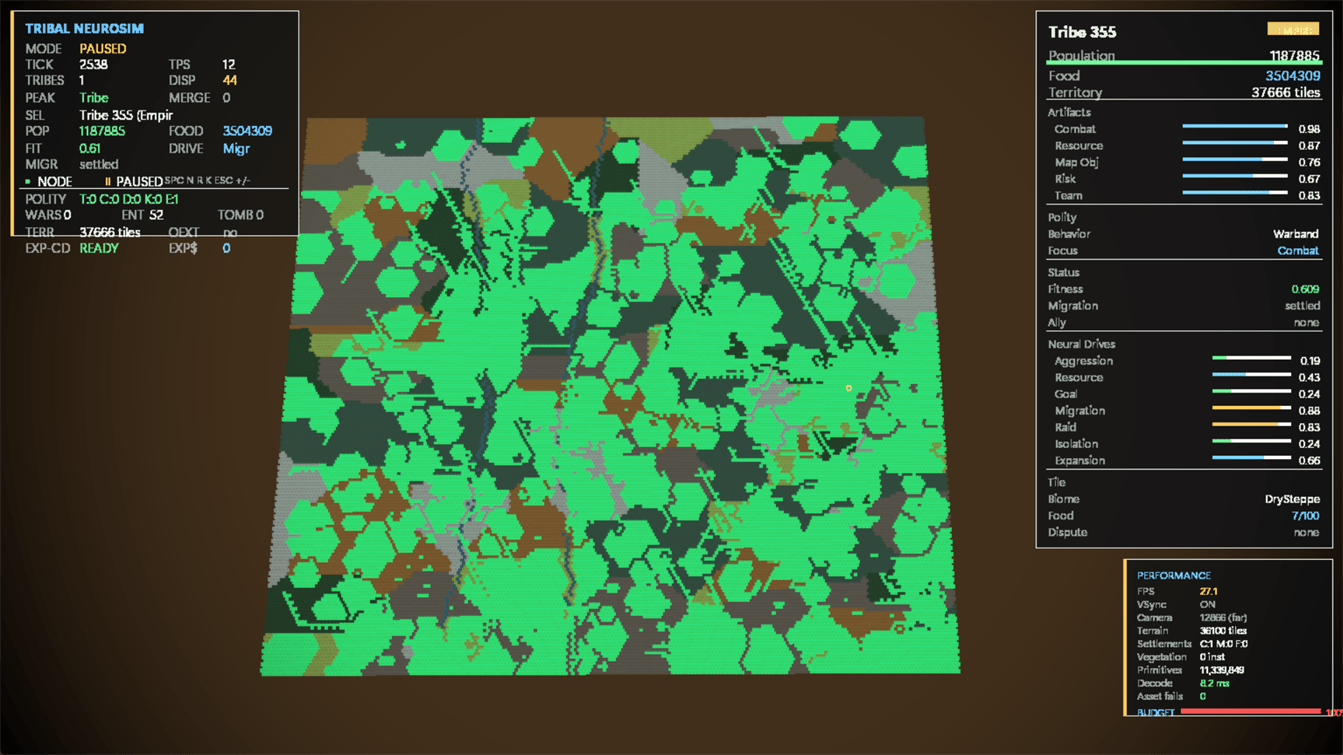
\includegraphics[width=0.9\textwidth]{assets/neurosim/run67fl7777-fl-s7777-tick2538-last.png}
  \caption{Flexset, seed=7777, tick=2538: a győztes Tribe~355 végső állapota.
    A\_combat=0{,}98 (telített maximumon) - 2538~tick harci tapasztalatának
    kumulált eredménye. Az inicializáláskor kapott klaszterprior és a futtatás
    végi érték közötti különbség az artifact felhalmozódási mechanizmus
    közvetlen mérése.}
  \label{fig:neurosim-fl7777-winner-final}
\end{figure}

\begin{figure}[h]
  \centering
  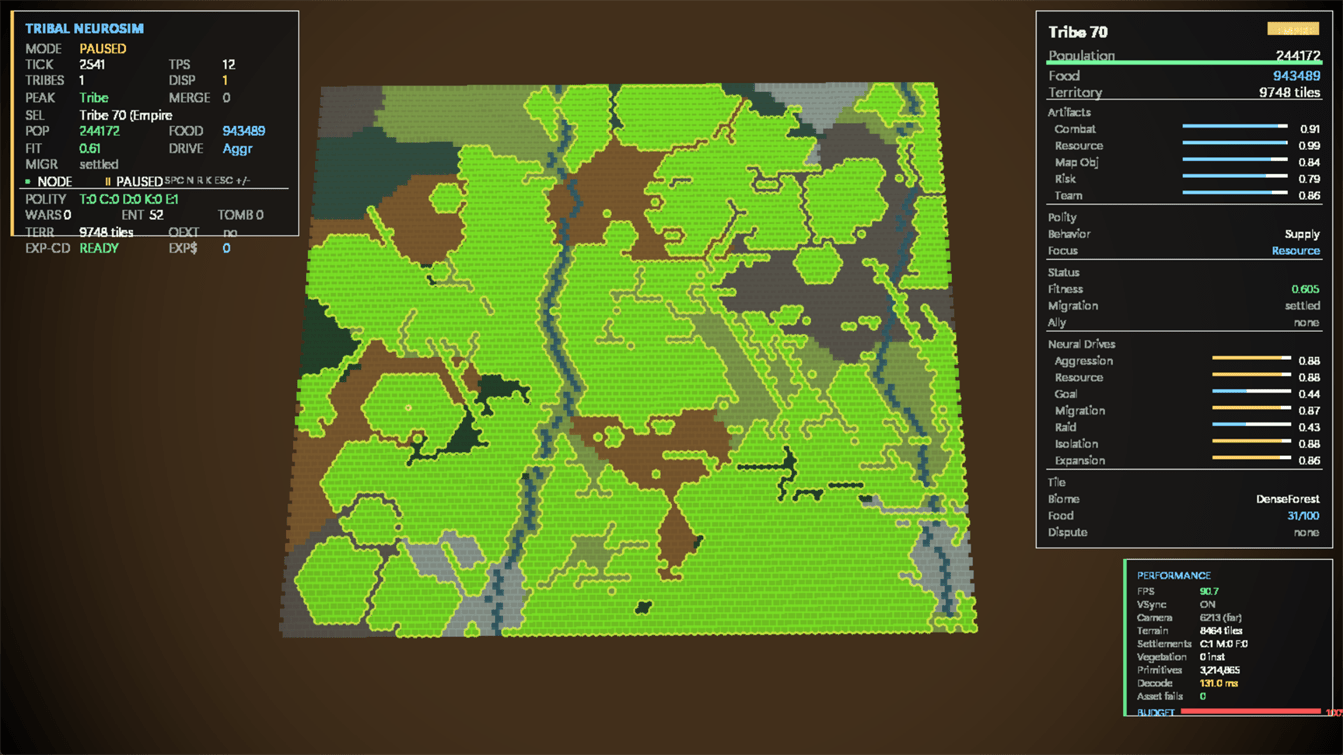
\includegraphics[width=0.9\textwidth]{assets/neurosim/run67sq7777-sq-s7777-tick2541-last.png}
  \caption{SoloQ, seed=7777, tick=2541: a győztes Tribe~70 eltérő artifact-profillal
    (Supply/Resource archetípus). Az eltérő adatkészletből induló törzs eltérő
    felhalmozódási mintát produkál azonos szimulációs szabályok mellett -
    a SoloQ klaszterstruktúra egyéni teljesítményorientációja a harci tapasztalat
    helyett a terület- és erőforrás-felhalmozásban mutatkozik meg.}
  \label{fig:neurosim-sq7777-winner-final}
\end{figure}

Az artifact felhalmozódás következménye, hogy a futtatási narratívákban (ld.~24.4~szekció)
megfigyelt győztesek viselkedési profilja nem pusztán a klaszter-derivált priorból ered,
hanem a szimuláció során szerzett tapasztalat és a genomevolúció együttes eredménye.
Ez a mechanizmus biztosítja, hogy a NeuroSim nem determinisztikusan másolja
a bemeneti klaszterprofilokat, hanem azokon \textit{evolúciós nyomás alatt} alapuló,
mérhetően eltérő kimeneteket produkál \cite{stanleymiikkulainen2002}, \cite{holland1992}.

% ============================================================
\section{Stratégiai interakció és konfliktusos struktúra}
\label{sec:neurosim-25-strategic}

A szimuláció minden stratégiai döntése - háborúindítás, szövetségkötés, visszavonulás,
vitatott területre való belépés, fuzionálás - olyan állapotátmenet, amelynek kimenetele
nem pusztán a döntést hozó törzs genomjától függ, hanem legalább annyira a szomszédos
entitás aktuális állapotától is. Ebből fakad, hogy a Tribal NeuroSim egyidejűleg
rendszer az evolúciós tanulásra és arra, hogy kölcsönösen függő döntések láncolatából
emergáló makroszintű minták keletkezzenek.

\subsection*{Bináris diplomácia és vitatott területek}

A V3-as architektúra diplomáciája szándékosan bináris: vagy \textit{totális háború},
vagy \textit{teljes szövetség és fuzionálás}. Részleges fegyverszünet, semlegességi
egyezmény, kereskedelmi megállapodás - ezek nem léteznek. Ez a tervezési döntés
magas tétű, determinisztikus konfliktusos struktúrát kényszerít ki: a neurális hálózatnak
minden szomszédra vonatkozóan el kell döntenie, hogy az adott entitás absorbálandó-e
a saját struktúrájába, vagy megsemmisítendő.

A tényleges futásokban a formális szövetség ritka kimenet maradt. A mechanika
fontos, mert lehetőséget ad a békés fuzionálásra, de a logok alapján a világ
többnyire abszorpcióval rendeződött: a domináns törzs vagy ellenállás után,
vagy ellenállás nélkül olvasztotta be a gyengébb szomszédot.

A területi modell szintén nyomást generál. Egy tile-ot egyszerre több törzs is igényelhet -
ilyenkor a tile \textit{vitatottá} válik, és mindkét törzs $-40\%$-os hatékonysági
büntetéssel szembesül. Ha Törzs~A 70\%-ot kontrolál egy vitatott tile-ból, tényleges
hozama $0{,}70 \times 0{,}60 = 0{,}42$, azaz a névleges igény 42\%-a. Ez a büntetés
belső egyensúly-zavaró erőként hat: a neurális hálózat kénytelen mérlegelni, hogy
a csökkentett hozamú közös használat még mindig kedvezőbb-e a háborúnál, vagy a
vita feloldásának - erővel vagy visszavonulással - van kisebb összköltése.
Az \texttt{A\_risk} artifact (\ref{tab:neurosim-inputs}.~táblázat, 10.~index)
közvetlenül befolyásolja ezt a mérlegelést: alacsony kockázattűrés esetén a törzs
hamarabb választja a konfrontációt a büntetett megosztott használat felett.

\subsection*{Opportunista és stagnálási háború}

Az opportunista háború mechanizmusa célirányos: \texttt{raid\_drive}~$> 0{,}35$
és \texttt{food\_ratio}~$> 0{,}5$ és létezik a térképen gyengébb szomszéd
(alacsonyabb \texttt{pop~$\times$~a\_combat} szorzattal) - ha mindhárom feltétel
teljesül, a törzs háborút indít a leggyengébb azonosított szomszéd ellen.
A szelektivitás szándékos: a magas \texttt{raid\_drive} nem jelent vaktában
agresszív viselkedést, hanem kalkulált opportunizmust. Ez egyezik a 23.2~szekcióban
ismertetett \texttt{raid\_drive}-\texttt{aggression} különbségtétellel: az előbbi
célzott, az utóbbi indiscriminate.

A stagnálási háború mechanizmusa ezzel szemben kényszert vezet be. Ha a szimuláció
meghatározott számú ticken át nem észlel egyetlen háborúdeklarációt sem, fokozatosan
növekvő háborús nyomás épül fel az összes élő törzsnél. Ez a nyomás előbb-utóbb
átlép egy küszöböt, és deklarációt vált ki - akkor is, ha az érintett törzsek genomja
önmagában nem indítaná el a konfliktust. A mechanizmus bevezetésének oka egyértelmű:
a V2-es prototípus korai futtatásaiban a törzsek egy részének genomja olyan izolacionista
és defenzív volt, hogy hosszú szakaszokon nem indult háború - a szimulált világ stabilis,
de befagyott állapotba kerül. A szimuláció lefutott, de végkimenetel nem keletkezett.
A stagnálási mechanizmus ezt a \textit{békés genomiális deadlockot} törte meg, és
biztosította, hogy minden futtatás konvergál egyetlen túlélőhöz.

\subsection*{Hawk-Dove értelmezési keret}

Maynard Smith és Price evolúciós játékelméleti keretrendszere \cite{maynardsmithprice1973},
\cite{maynardsmith1982} kínál egy értelmezési vonatkoztatási pontot a megfigyelt
viselkedési mintákhoz: a magas \texttt{raid\_drive} és magas \texttt{aggression}
kombinációja Hawk-típusú viselkedési pozícióként azonosítható - a törzs aktívan keresi
a konfliktust és maximalizálja az erőforrásfoglalást. A magas \texttt{isolation} és magas
\texttt{goal\_drive} kombinációja ezzel szemben Dove-típusú pozíciónak tekinthető:
a törzs kerüli a közvetlen konfrontációt, és belső fejlesztésre összpontosít.
Hangsúlyozni kell azonban, hogy ez \textit{viselkedési megfigyelés}, nem megoldott
evolúciós egyensúly: a szimuláció nem implementálja a Hawk-Dove kifizetési mátrix
formális struktúráját, és az itteni alkalmazása analógiaként, nem modellként értendő.

\subsection*{Négy konkrét futtatási eset}

Az alábbi táblázat összefoglalja a négy futtatás legjellemzőbb konfliktusos eseményét,
majd minden esethez egy rövid magyarázat következik.

\begin{table}[h]
  \centering
  \small
  \caption{Konfliktusos struktúra-típusok a négy futtatásban.}
  \label{tab:neurosim-conflict-cases}
  \resizebox{\textwidth}{!}{%
  \begin{tabular}{llp{4.5cm}p{4cm}}
    \hline
    \textbf{Futtatás} & \textbf{Tick} & \textbf{Esemény} & \textbf{Struktúra típusa} \\
    \hline
    Flexset 7777 & 2040 &
      55 egyidejű opportunista háború; 68→13 élő $\approx$210 tick alatt &
      Hawk–Hawk kaszkád \\
    Flexset 42 & 2400 &
      tribe\_90 és tribe\_596 egymástól függetlenül, egyszerre azonosította
      tribe\_557-et célpontként &
      Trilaterális – kétoldalú Hawk a domináns ellen \\
    SoloQ 42 & 1926–1935 &
      tribe\_89 egymás után 3 védelmi háborút nyert
      (tribe\_132, tribe\_36, tribe\_130) &
      Dove-erőd: Hawk-ok visszaverve \\
    SoloQ 7777 & 387–2340 &
      tribe\_99 sorozatosan 7 háborút nyert,
      majd tick=2340-en tribe\_45 legyőzte &
      Domináns Hawk felborulása \\
    \hline
  \end{tabular}
  }
\end{table}

\textbf{Flexset 7777, tick 2040 - Hawk-Hawk kaszkád.}
A nagy háborúban 55 törzs indított opportunista háborút egyetlen ticken belül.
A kaszkád oka a szimultán opportunitás-küszöb-teljesülés: az összes megmaradó Empire
egyszerre azonosított gyengébb szomszédot, és a 23.2~szekcióban leírt feltételek
mindannyiuknál egyszerre teljesültek. Az eredmény: 68 élőről 13-ra csökkent a mező
$\approx$210 tick alatt (tick 2043-tól tick 2250-ig). A kaszkád nem egyetlen esemény
következménye volt - a győztesek is elvesztítottek populációt és erőforrásokat,
majd az így meggyengült pozíciókra újabb deklarációk következtek.

\textbf{Flexset 42, tick 2400 - trilaterális struktúra.}
Tribe~557 kb. 23~000 tile-ra nőtt, miután tick~2352-en abszorbeálta tribe\_435-öt.
Erre reagálva tribe\_90 (raid=0{,}27, aggr=0{,}84) és tribe\_596 (raid=0{,}31,
aggr=0{,}13) egymástól teljesen függetlenül azonosítottak a domináns entitást
célpontként, és ugyanazon ticken háborút indítottak ellene.
Ez nem formális szövetség volt: mindkét törzs saját opportunitás-kalkulációja
vezette a döntéshez, amelyek véletlenszerűen egybeestek.
Tribe\_596 nyerte a háborút tick=2424-en; a kétfrontos nyomás döntő szerepet
játszott abban, hogy tribe\_557 - amelyik egyébként a legnagyobb területet kontrollálta -
nem tudott védekezni. Az artifact felhalmozódás szempontjából (ld.~23.3~szekció)
ezt az eseményt a \texttt{A\_combat} értékek is tükrözik: tribe\_596 védelmi
győzelmei tickek százain át formálták azt a harci tapasztalatot, amellyel a
döntő pillanatban nyert.

\textbf{SoloQ 42, ticks 1926-1935 - Dove-erőd.}
Tribe\_89 alacsony agresszióval (0{,}11) és magas \texttt{raid\_drive}-val (0{,}84)
kombinált Vanguard viselkedési profilt mutatott. Tick~1926-ban tribe\_132 támadta meg;
tribe\_89 védekezőként nyert. Tick~1935-ben tribe\_36 és tribe\_130 egyszerre támadott -
mindkettő ugyanabban a tickben halt meg, miközben tribe\_89 védekező pozíciójából
nem mozdult. A három egymást követő védelmi győzelem 9 ticken belül azt illusztrálja,
hogy a 23.2~szekcióban ismertetett \texttt{isolation} hajtóerő (0{,}68)
kombinálva a magas raid-képességgel erős defenzív pozíciót teremt: a törzs nem
szövetkezett, nem menekült, és nem kezdeményezett - de az összes beérkező Hawk-típusú
támadást visszaverte.

\textbf{SoloQ 7777, ticks 387-2340 - domináns Hawk felborulása.}
Tribe\_99 a szimulált világ 1500 tickjén keresztül volt az egyértelműen domináns
offenzív aktor, sorozatban legyőzve tribe\_76-ot (tick~387), tribe\_61-et (tick~1239),
tribe\_101-et (tick~1392), tribe\_92-t (tick~1692), tribe\_85-öt (tick~1935) és
tribe\_124-et (tick~2091) - összesen 7 egymás utáni győzelem.
Tick~2340-en tribe\_45 támadta meg és legyőzte - a dominancia összeomlott.
A tényleges győztes, tribe\_70, csendesen gyűjtötte a területet és túlélte az
ellene irányuló védelmi próbálkozásokat, majd a végső párbajon nyert tick=2541-en.
Ez a minta - domináns Hawk akumulálja a győzelmeket, majd egyetlen vereség mindent
elvesz - a SoloQ futtatásra jellemző, és nem jelent meg egyik flexset futtatásban sem,
ahol a konszolidáció elosztott volt, és nem egyetlen domináns aktor keretezte.

\begin{figure}[h]
  \centering
  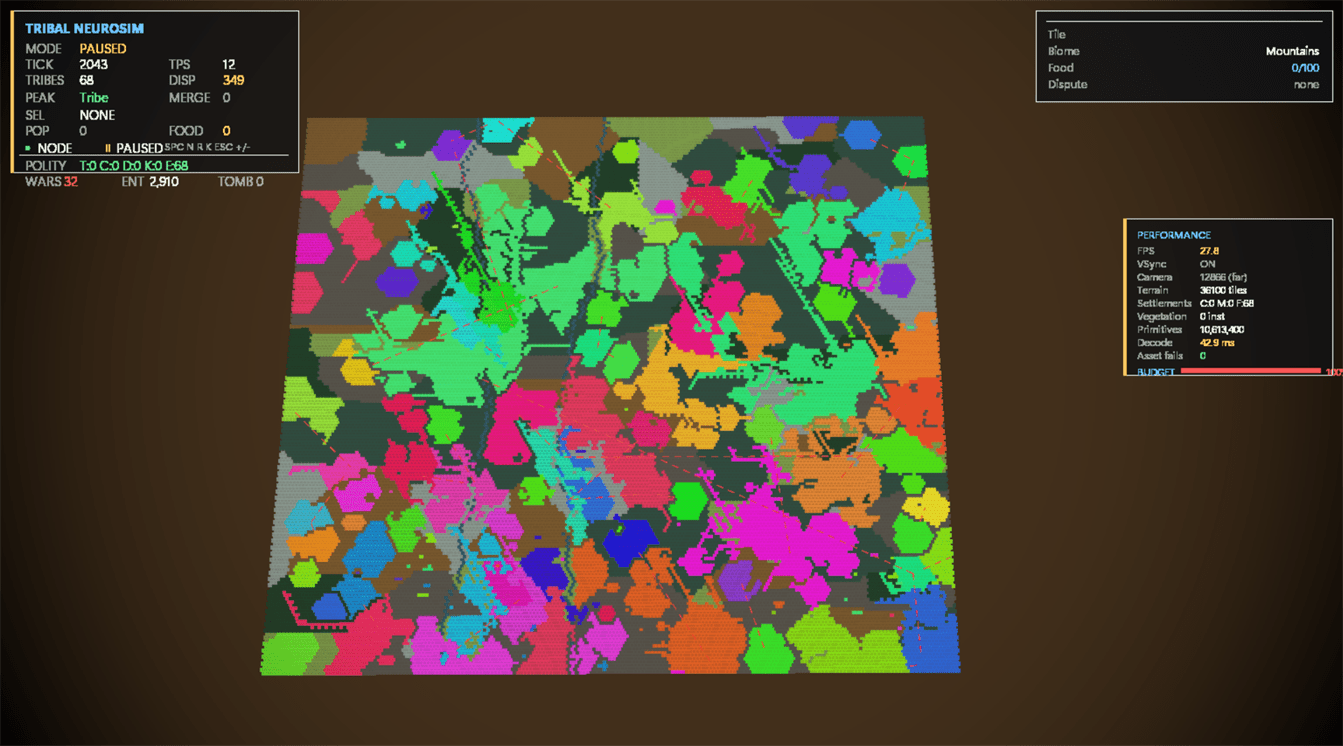
\includegraphics[width=0.9\textwidth]{assets/neurosim/run67fl7777-fl-s7777-tick2043-totalwar.png}
  \caption{Flexset, seed=7777, tick=2043: 68 élő törzs, 32 egyidejű aktív háború.
    Az összes visszamaradt entitás Empire-szinten van - a Hawk-Hawk kaszkád csúcspontja,
    három tickkel az 55 szimultán deklaráció után.}
  \label{fig:neurosim-fl7777-totalwar}
\end{figure}

\begin{figure}[h]
  \centering
  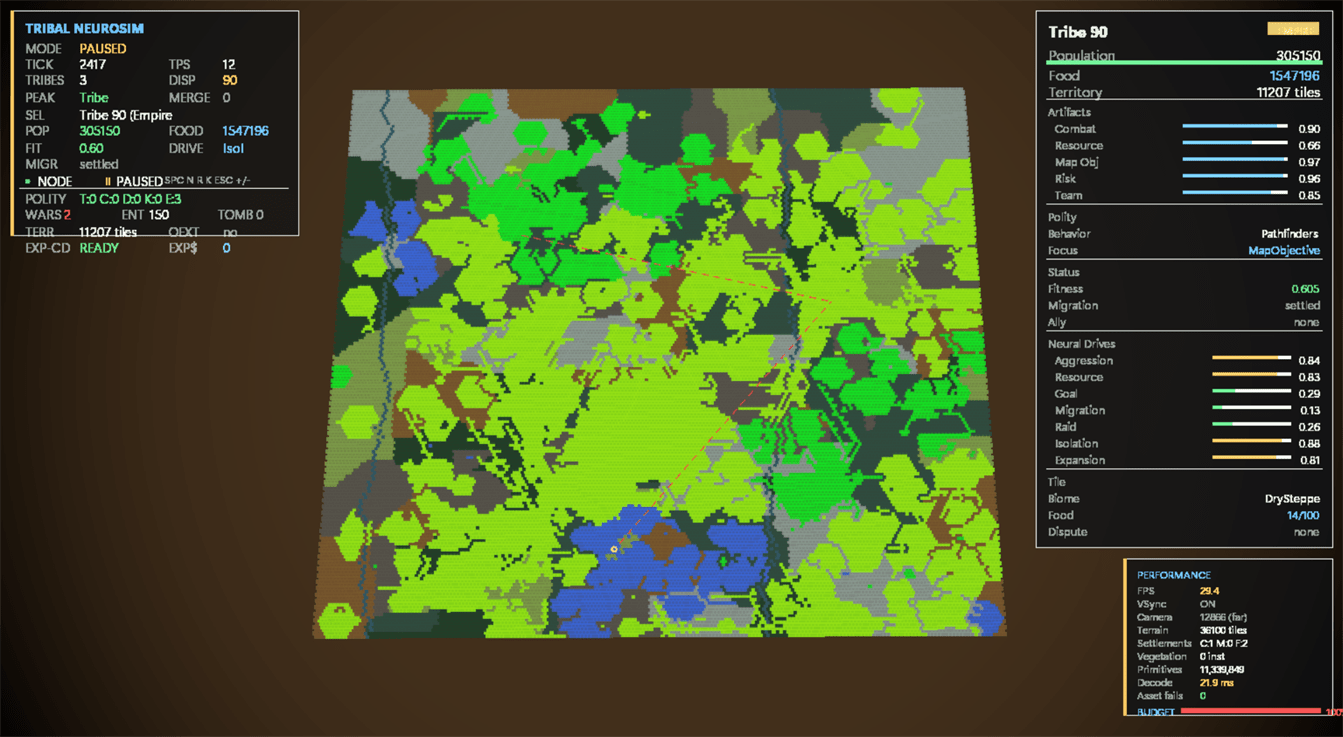
\includegraphics[width=0.9\textwidth]{assets/neurosim/run67fl42-fl-s42-tick2417-trilateralwar.png}
  \caption{Flexset, seed=42, tick=2417: trilaterális háború. Tribe~90 (11~207 tile,
    aggr=0{,}84) és tribe~596 (aggr=0{,}13) egymástól függetlenül egyszerre
    azonosította tribe~557-et ($\approx$23~000 tile) célpontként - nem formális
    szövetség, hanem párhuzamos opportunitás-kalkuláció eredménye.}
  \label{fig:neurosim-fl42-trilateral}
\end{figure}

\subsection*{Konfliktusos struktúrák összefoglalása}

A fentebb azonosított konfliktusos struktúra-típusok - kaszkád, trilaterális nyomás,
defenzív erőd, domináns aktor felborulása - nem pusztán egyedi epizódok; a négy
futtatás eseménynaplói azt mutatják, hogy ezek a minták az adatkészlet és a seed
függvényében reprodukálható következetességgel jelennek meg. A 24.~fejezet futtatási
narratívái ezeket a konfliktusos mintákat konkrét eseménynaplók alapján dokumentálják,
és összefoglalják, mit támasztanak alá és mit nem bizonyítanak a megfigyelt eltérések
a flexset és a SoloQ adatkészlet között.

\bigskip

% ===== chapters/24-tribal-neurosim-futtatások-validacio-es-ertelmezés.tex =====
\chapter{Tribal NeuroSim - Futtatások, validáció és értelmezés}

\section{Világ-mechanikák és térbeli szubsztrát}
\label{sec:neurosim-26-mechanics}
% ==========================================================================

\subsection*{Hex-rácsvilág és biome-ok}

A szimuláció terét egy hexagonális rács alkotja, amelyben minden tile-nak legfeljebb hat szomszédja van. Ez a topológia egy térbeli gráf: a törzsek terjeszkedési útjai és stratégiai határai a szomszédsági reláción alapulnak, amelynek elvi háttere a 12-13.~fejezetekben tárgyalt pathfinder-architektúrában gyökerezik; itt a rács kizárólag mint szimulációs szubsztrátum kerül bemutatásra.

A világ mérete adatkészlet-függő. A flexset adatkészletből inicializált futtatások $\approx$36\,100 tile-os térképen játszódnak, mivel a Flex Queue klaszterpopuláció nagyobb és geográfiailag szétszórtabb. A SoloQ futtatások kisebb világokat kapnak; a vizsgált két SoloQ futtatás végső győztes területe 6\,356 és 9\,748 tile volt. Ez sűrűbb kezdeti törzsközeli elhelyezkedést és gyorsabb korai konszolidációt eredményezhet - amint az a~\ref{fig:neurosim-sq7777-tick301} ábrán is látható.

Minden tile-hoz egy biome-típus van rendelve, amely meghatározza az alap élelmiszertermelési rátát és mozgási tulajdonságokat:

\begin{table}[h]
\centering
\caption{Biome-típusok és élelmiszertermelési jellemzőik}
\label{tab:biomes}
\begin{tabular}{lll}
\hline
\textbf{Biome} & \textbf{Termelési szint} & \textbf{Különleges tulajdonság} \\
\hline
DenseForest & Magas        & Alapbiome; stabil élelmiszer-alap \\
Riverland   & Közepes      & Halászati bónusz ($+25\%$ folyóval szomszédos tile-okra) \\
DrySteppe   & Alacsony     & Alacsony foglalási költség, gyors terjeszkedés \\
Mountains   & Nulla        & Áthatolhatatlan - természetes terjeszkedési barrier \\
Marsh       & Alacsony     & Mozgásgátló, magasabb foglalási költség \\
Cold        & Nagyon alacsony & Populáció-fenntartás kritikus szint közelében \\
\hline
\end{tabular}
\end{table}

A biome-ok nem csupán passzív háttér: a törzs A\_resource artifaktuma közvetlenül modulálja, hogy mennyire hatékonyan tudja kiaknázni az adott biome potenciálját. Egy alacsony A\_resource értékű törzs DenseForest tile-on is szuboptimálisan teljesíthet, míg egy magas A\_resource értékű törzs DrySteppe-en is fenntartható szinten maradhat - bár ez utóbbi esetben a terjeszkedési kényszer szinte elkerülhetetlen.

\begin{figure}[h]
\centering
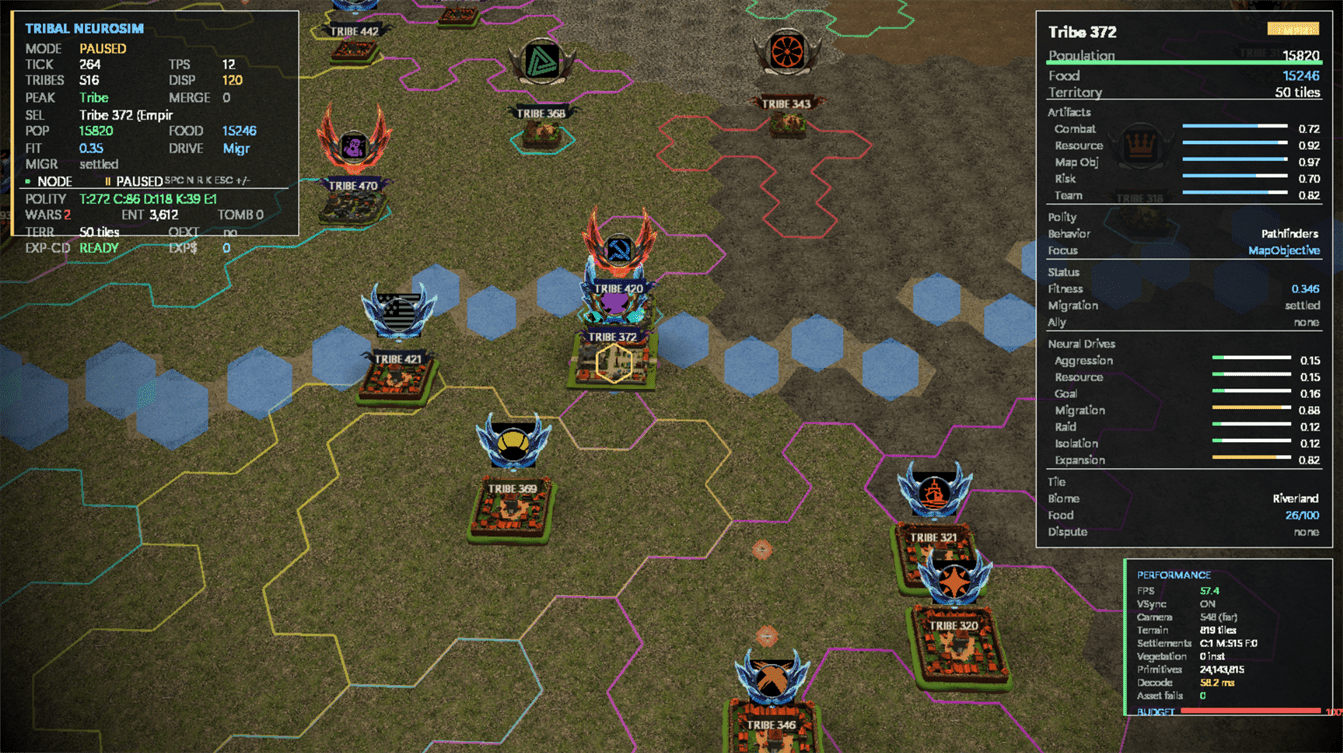
\includegraphics[width=0.9\textwidth]{assets/neurosim/run67fl7777-fl-s7777-tick264-firstempire.png}
\caption{Flexset, seed=7777, tick=264: közeli nézet a hex-rácson. Tribe~372 tile-jai körül biome-váltás (Riverland → DenseForest) látható; az egyes tile-ok élelmiszertermelési kapacitása biome-specifikus.}
\label{fig:neurosim-fl7777-tick264}
\end{figure}

\begin{figure}[h]
\centering
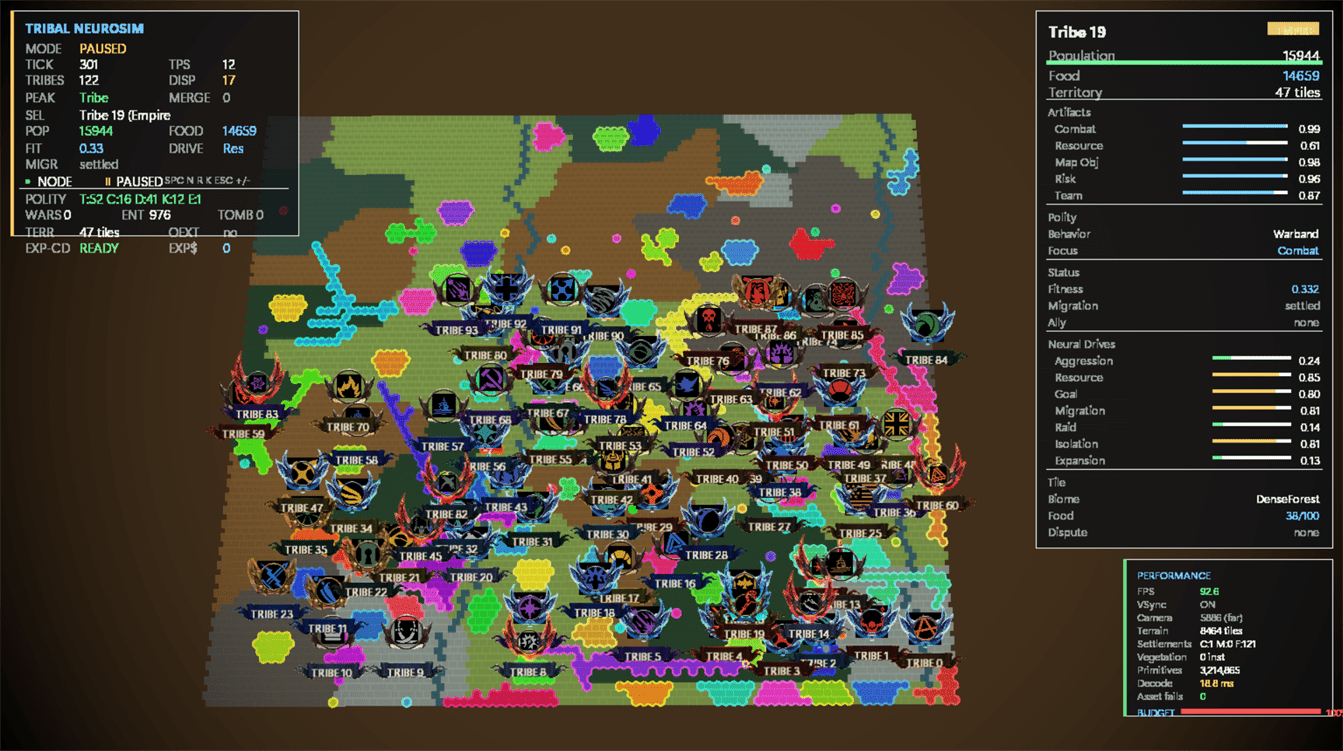
\includegraphics[width=0.9\textwidth]{assets/neurosim/run67sq7777-sq-s7777-tick301-firstempire.png}
\caption{SoloQ, seed=7777, tick=301: a kisebb soloq világ sűrűbb kezdeti elhelyezkedést és gyorsabb korai konszolidációt eredményez.}
\label{fig:neurosim-sq7777-tick301}
\end{figure}

\subsection*{Tile-tulajdonlás, vitatott zónák és terjeszkedési költség}

A v3-as architektúra bevezette a törtrészes tile-irányítás modelljét (TaskR4, 2026-05-06). Az egyes tile-ok nem bináris „1 vagy 0" alapon kerülnek hozzárendelésre; egyszerre több törzs is fennhatóságot tarthat rajtuk, törtrészes arányban, amelyet egy kompakt Rust adatstruktúra tárol:

\begin{lstlisting}[language={}, caption={Tile-irányítás adatstruktúra (részlet, TaskR4)}]
struct TileControl {
    tribe_id: u32,
    control_percentage: f32,  // pl. 0.70 = 70%-os irányítás
}
// Legfeljebb 4 törzs per tile, memóriahatárral
tile_occupants: Vec<ArrayVec<TileControl, 4>>
tile_is_disputed: Vec<bool>
\end{lstlisting}

\textbf{A vitatott zóna mechanikája:} ha két vagy több törzs ugyanazon a tile-on osztozik, a tile \textit{Disputed} státuszba kerül, és azonnali $-40\%$-os hatékonysági büntetés lép életbe minden ott végzett műveletre. A nettó erőforrás-hozam:

\begin{equation}
\text{nettó\_hozam} = \text{control\_percentage} \times (1{,}00 - 0{,}40)
\end{equation}

Ha például egy törzs egy vitatott tile-on 70\%-os irányítást tart fenn, a tényleges hozam $0{,}70 \times 0{,}60 = 0{,}42$, vagyis 42\%. Ez a matematikai kényszer természetes \textit{casus bellit} kelt: a törzs neurális hálózatának folyamatosan értékelnie kell, hogy a büntetett hozam elegendő-e a fennmaradáshoz, vagy erőszakos feloldásra van szükség.

A vitafeloldás három úton lehetséges, amelyeket a szimuláció 30 tickenként futtat: (1) \textit{passzív elfogadás}, ha az A\_risk artifaktum értéke $> 0{,}70$ és a büntetetett hozam meghaladja a túlélési küszöböt; (2) \textit{katonai fenyegetés}, ha az A\_combat értéke $> 0{,}80$ és magasabb, mint az ellenfélé - ekkor az ellenfél kénytelen visszavonulni; (3) \textit{diplomáciai fuzionálás}.

A terjeszkedés sebességét és költségét a TaskR8 (2026-05-07) implementáció rögzíti.
Minden foglalást egy per-törzs 25 tickes visszaszámlálás korlátoz; az igénylés csak
akkor hajtható végre, ha a következő két feltétel egyszerre teljesül:

\begin{equation}
\text{pop} \geq 80 + 25 \times |\mathcal{T}_i|
\quad \text{és} \quad
\text{food} - \text{cost}(\text{tile}) \geq 50
\end{equation}

ahol $|\mathcal{T}_i|$ az $i$-edik törzs jelenleg irányított tile-jainak száma,
a $\text{cost}(\text{tile})$ az adott biome foglalási költsége.
Újonnan foglalt tile-ok 75 tickes integrációs perióduson mennek keresztül,
amelynek során a hozam lineárisan emelkedik:

\begin{equation}
h(t) = h_{\max} \cdot \frac{t - t_0}{75}, \quad t_0 \leq t \leq t_0 + 75
\end{equation}

ahol $h_{\max}$ a biome nominális hozama és $t_0$ a foglalás tick-je.
Overextension akkor lép fel, ha az irányított tile-ok száma meghaladja
a fenntartható korlátot:

\begin{equation}
|\mathcal{T}_i| > 1 + \left\lfloor \frac{\text{pop}}{120} \right\rfloor
\quad \Rightarrow \quad \Delta\text{cost} = +10 \text{ egység/foglalás}
\end{equation}

\subsection*{Populáció és erőforrásmodell}

A törzs populációja és élelmiszer-készlete tickenként kölcsönösen hat egymásra. Az élelmiszerfogyasztás arányos a populációval; ha a fogyasztás meghaladja a termelést, az éhhalál mechanizmusa csökkenti a populációt. A \texttt{resource\_drive} hajtóerő - amelynek értelmezése a 23.2.~alszekciójában kerül kifejtésre - modulálja a gyűjtési rátát: magas értékű törzsek aktívabban keresnek élelmiszer-forrást, alacsony értékű törzsek a harci vagy migrációs prioritások miatt elfogadják az alacsonyabb gyűjtési hatékonyságot.

A fenntartható egyensúly feltétele:
\begin{equation}
\text{populáció} \times \text{fogyasztás/fő} \;\leq\; \text{terület} \times \text{biome\_ráta} \times A\_\text{resource}
\end{equation}

Ha ez a feltétel hosszabb ideig sérül, a törzs elveszíti terjeszkedési képességét, majd - az éhhalál spiráljában - a fennmaradási képességét is. A szimuláció egyik fő szelekciós nyomása tehát nem a harci erő, hanem az erőforrás-egyensúly fenntartása.

\subsection*{Harci mechanika}

Minden háborús ticken Poisson-elosztású harci körök zajlanak le. Az eredményt az ütköző felek A\_combat artifaktumainak összevetése határozza meg: a magasabb harci profil magasabb valószínűséggel kényszeríti vissza az ellenfelet a magtile-okra. A háború három feltétel bármelyikének teljesülésével érhet véget: (1) az egyik fél összes tile-ját visszafoglalják és a törzs megsemmisül; (2) az egyik fél visszahúzódik a magtile-okra és megszűnik szomszédos lenni az ellenféllel; (3) mindkét fél a saját területére szorul - ekkor tüzszünet lép életbe.

A Poisson-elosztású harci körök matematikai modellje:

\begin{equation}
P(k \text{ találat}) = \frac{\lambda^k e^{-\lambda}}{k!},
\quad \lambda = a_{\text{att}} \cdot n_{\text{tiles}} \cdot 0{,}02
\end{equation}

ahol $a_{\text{att}}$ a támadó A\_combat artifaktuma, $n_{\text{tiles}}$ a
kontaktus-tile-ok száma, és a $0{,}02$ az alap harci szorzó.
A várható veszteség ezért $\mathbb{E}[k] = \lambda$; magas A\_combat és széles
kontaktzóna esetén a veszteség gyorsabban akkumulálódik, ami statisztikailag
előbb vezet teljes elfoglaláshoz, mint tárgyalásos visszavonuláshoz.
Ez magyarázza, miért végződik a legtöbb háború totális elfoglalással, nem
tűzszünettel: a Poisson-folyamat nem konvergál a halasztáshoz.

Az opportunista raid mechanizmus (raid\_drive $\times$ opportunity\_score $>$ küszöb) lehetővé teszi, hogy egy törzs akkor is háborút kezdeményezzen, ha még nem ért el katonai fölényt - például ha az ellenfél éppen más fronton harcol. Ez az algoritmus közvetlen felelős a 23.4.~alszekciójában bemutatott kaszkádjelenségekért: a flexset seed=7777 futtatás tick=2040-es Totális Háborújában 64 egyidejű opportunista háború indult, és a tick=2050-nél mért 63 élő törzsből tick=2250-re már csak 13 maradt.

A harci körök kimenetének statisztikai következménye, hogy a legtöbb háború
totális elfoglalással végződik, nem tűzszünettel. A Poisson-folyamat nem
konvergál az egyensúlyi megosztáshoz: ha $\lambda > 0$ fennáll minden harci
tick-en, a kumulált veszteség előbb-utóbb az egyik fél teljes összeomlásához
vezet. Mérsékelt $A_{\text{combat}}$ különbség esetén ez 50--200 tick-et vesz igénybe;
nagy különbség esetén (pl. 0{,}98 vs.\ 0{,}45) 10--30 tick is elegendő.
Ez a mechanika a szimuláció egyik erős kaosz-faktora: a látszólag stabil
kétpólusú helyzet megtörhet, ha egy harmadik törzs opportunista háborút indít
miközben az egyik fél már harci veszteséget szenved el.

\subsection*{Polity-szintek és fejlődési feltételek}

A törzsek hierarchikus politikai entitásokká fejlődhetnek, ha egyszerre teljesítik a populációs, területi és neurális küszöbfeltételeket. A fejlődési lépcsőfok:

\begin{table}[h]
\centering
\caption{Polity-szintek és közelítő fejlődési feltételek}
\label{tab:polity}
\begin{tabular}{lllll}
\hline
\textbf{Szint} & \textbf{Populáció} & \textbf{Terület} & \textbf{goal\_drive} & \textbf{Megjegyzés} \\
\hline
Tribe   & $\geq 80$    & $\geq 1$ tile    & -              & Kezdeti állapot \\
City    & $\geq 200$   & $\geq 5$ tile    & $> 0{,}40$     & Első settlement nyílik \\
Duchy   & $\geq 500$   & $\geq 15$ tile   & $> 0{,}55$     & Regionális dominancia \\
Kingdom & $\geq 1200$  & $\geq 40$ tile   & $> 0{,}65$     & Fuzionálási képesség \\
Empire  & $\geq 3000$  & $\geq 100$ tile  & $> 0{,}75$     & Végső győzelmi státusz \\
\hline
\end{tabular}
\end{table}

A settlement modell a polity szinthez kötött: minden szintlépés egy-egy settlement-csomópontot nyit meg a vizuális felületen. A MonoGame HUD-ban például a \texttt{C1 M0 F12} jelölés azt jelenti, hogy az adott törzs 1 várossal, 0 erőddel és 12 farmmal rendelkezik - ezek a fejlettségi mutató közvetlen leolvasási pontjai. A settlement-szám egyszerre tükrözi a polity szintet és az erőforrás-infrastruktúra méretét.

\subsection*{Szövetség, fuzionálás és kihalás}

A diplomácia bináris, amint azt a 23.4.~alszekció részletezi: vagy teljes háború, vagy kölcsönös szövetség, esetleg fuzionálás. Szövetség esetén a felek megnemtámadási jelzést adnak a neurális bemenetükre, de önállóak maradnak - a \texttt{legközelebbi\_szövetséges\_távolsága} bemeneti jel csökken, ami alacsonyabb isolation- és magasabb csapatkoordinációs nyomást jelent. A javított futásokban ezek a formális szövetségek ritkák: a rendszer inkább abszorpciós végjátékot produkál, ahol a nagyobb törzs ellenállással vagy ellenállás nélkül olvasztja be a kisebbet. Fuzionálás feltétele mindkét félnél: goal\_drive $> 0{,}55$, egyik sem áll éppen háborúban, és isolation $< 0{,}75$. Fuzionáláskor a két genomot fitnesz-súlyozott örökléssel vonják össze (lásd 23.3.~alszekció).

Kihalás esetén a törzs összes tile-ját visszafoglalják, majd tombstone rekord rögzíti az utolsó állapotot: genomot, leszármazást, harci rekordot és a kihalás okát. A leszármazási DAG - ahol minden törzs szülői linkeket tárol, nem teljes ancestry stringeket - technikailag egy irányított aciklikus gráf. A hex szomszédosság és a leszármazási lánc egyaránt gráf-struktúra; mindkét fogalom elvi háttere a 12-13.~fejezetekben kerül kifejtésre; itt kizárólag a szimulációs tartományra vonatkozó mechanikai alkalmazásuk releváns.

% ==========================================================================
\section{Iteratív újratervezés és hibaelőzmények}
\label{sec:neurosim-26-redesign}
% ==========================================================================

A Tribal NeuroSim v3-as, thesis-érett formája nem egyetlen tervezési iterációban jött létre. A rendszer jelenlegi állapota több prototípusgeneráció tanulságain, kritikus újratervezési döntéseken és célzott hibajavítási ciklusokon keresztül alakult ki. Ez az alszekció dokumentálja a korai verziók meghibásodásait, az ezekre adott architektúrális válaszokat és a liveness-fix során azonosított specifikus numerikus hibákat - mindezek nélkül a v3 futtatások validitása nem értelmezhető.

\subsection*{V1/V2 webes prototípus hibái}

A rendszer első, böngészőalapú prototípusa (v1/v2) egy React/Node frontend és egy Rust backend kombinációjaként futott, WebSocket streamen keresztül. Az első teljes futtatás post-mortem dokumentuma kilenc klinikai fázist azonosított, amelyek együttesen kritikus architektúrális hiányosságokat jeleztek.

\textbf{Inicializációs hiba (tick=21):} Az 599 törzs négy sűrű sorban jelent meg a térkép egy szűk sávjában; az élelmiszer-spawn rutin nem futott le. Minden törzs éhezési állapotban inicializálódott.

\textbf{Szellemháborúk (tick=257):} A harci állapotgép nem zárta le a befejezett háborúkat. Tick=257-re 323 aktív háború volt nyilvántartásban, miközben a teljes populáció ennél jóval kisebb volt - statisztikailag lehetetlen szám. Tick=3085-re egyetlen élő törzs maradt, mellette 182 aktív szellemháborúval. A probléma mélyebb oka az volt, hogy nem létezett strukturált háborúlezárási esemény: a háborús rekordok soha nem kaptak „lezárt" státuszt, ezért a rendszer mindet aktívnak tartotta. Ahogy a 22.3.~alszekció tárgyalja, az eseménybusz hiánya tette ezt a hibát láthatatlanná - a tick=187-es tömeges kihalásnak semmi nyoma nem maradt a naplóban.

\textbf{Migrációs státuszblokkada (tick=342-832):} A törzs állapotgépe „Migrating" státusba kerülhetett anélkül, hogy a tényleges térbeli koordinátái változtak volna. A heurisztikus célpont-keresés minden szomszédos tile-t egyenlőnek értékelt (élelmiszer=0 mindenhol), így az A* útkeresés null utat adott vissza, és a törzs helyben maradt. Tick=342-re a túlélő törzsek ~90\%-a migrációs állapotban volt, tényleges mozgás nélkül. Tick=832-re az éhhalál megsemmisítette a populáció döntő részét.

\textbf{Memóriaszivárgás (tick=2842):} A meghalt törzsek aktív objektumként maradtak a memóriában, azok állapotát a garbage collector nem szabadította fel. Tick=2842-nél a böngészőfelület teljesen megfagyott - a szimulációs vezérlők (pause, god-mode) nem reagáltak. A futtatás tick=3085-nél ért véget, egyetlen életben maradt törzs 3. generációs elérésével.

\subsection*{Kritikus újratervezési döntések}

A post-mortem analízis öt architektúrális döntést tett kötelezővé:

\begin{enumerate}
  \item \textbf{Rust authority:} A teljes szimulációs logika Rust-ba kerül. A frontend kizárólag renderelési kliens - nem fut szimulációt, nem tárol érdemi állapotot.
  \item \textbf{Kötelező eseménybusz:} Minden állapotátmenet strukturált eseményt bocsát ki, append-only naplóba. A végső térképállapot önmagában nem bizonyíték - az audit trail kötelező.
  \item \textbf{Tombstone ledger:} Minden kihaló törzs tombstone rekordot kap (kihalási ok, utolsó genom, leszármazás, utolsó populáció és területszám). A szellemháborúk megszüntetésének feltétele, hogy a halál pillanatában az összes aktív háborúra \texttt{WarCancelled} esemény kerüljön.
  \item \textbf{Területi modell overhaul:} Bináris tile-tulajdonlás helyett törtrészes irányítás (lásd 24.1.~alszekció), vitatott zónák és terjeszkedési költségmodell.
  \item \textbf{MonoGame desktop kliens:} A böngésző prototípus memóriaszivárgásra hajlamos; a MonoGame C\# kliens FrameV1 bináris protokollon csatlakozik a Rust szerverhez, determinisztikus tick-szinkronnal.
\end{enumerate}

Ezek mellé két gameplay-szintű javítás is bekerült: az \textit{opportunista háborúmechanizmus} (raid\_drive × opportunity\_score alapú küszöb) és a \textit{stagnálási háborúmechanizmus} (ha N ticken nincs háborús aktivitás, nyomás épül fel), amelyek együttesen megakadályozzák a békés genomiális deadlock kialakulását - azt a jelenséget, amelynél minden törzs izolálódik és a szimuláció nem konvergál győztesre.

\subsection*{Task futtatási összefoglaló}

A v3-as rendszer implementációja diszkrét task-futtatásokon keresztül zajlott. Az alábbi táblázat összefoglalja a thesis szempontjából releváns feladatokat:

\begin{table}[h]
\centering
\caption{Implementációs task összefoglaló - kiemelt v3 futtatások}
\label{tab:tasks}
\begin{tabular}{llp{8cm}}
\hline
\textbf{Task} & \textbf{Dátum} & \textbf{Fő változás} \\
\hline
TaskR1 & 2026-05-06 & LineageRegistry (DAG ID rendszer); seed-entitás regisztráció; O(1) szülőlánc-lekérdezés \\
TaskR2 & 2026-05-06 & TombstoneLedger; ghost-war javítás (\texttt{WarCancelled} státusz); halott törzsek ~100 byte-os rekordra csökkentve \\
TaskR4 & 2026-05-06 & Törtrészes tile-irányítás; \texttt{TileControl} struktúra; vitatott zóna $-40\%$ büntetés \\
TaskR7 & 2026-05-06 & FrameV1 bináris protokoll; TNS3 envelope; little-endian; tile, háborús és esemény-delta szekciók \\
TaskR8 & 2026-05-07 & Hex-távolság; tereptől függő foglalási cost; overextension büntetés; 75 tickes integrációs periód \\
TaskM1 & 2026-05-08 & C\# FrameV1 dekóder; TNS3 envelope-parsírozás; backward-compatible V0 fallback \\
TaskM3 & 2026-05-08 & Hat-élű pointy-hex geometria; territory border rendering; Civ6-stílusú határvonal és crosshatch \\
TaskM9 & 2026-05-10 & MonoGame integráció; leszármazási inspektor panel (L); tombstone panel (K); HUD panelek \\
\hline
\end{tabular}
\end{table}

\subsection*{Liveness-fix részletei}

Az első teljes v3 futtatás (2026-05-14, 0-777 tick) statikusnak bizonyult: 599 törzs egyike sem halt meg, egyetlen háború sem zárult le, minden törzs pontosan 1 tile-t tartott fenn. A diagnózis három egymást erősítő hibát tárt fel.

\textbf{1. Kétszeres normalizálás:} A \texttt{server.js} már 0-1 közé normalizálta az artifaktum-értékeket (osztás 4,5-tel vagy 5,0-val). A Rust \texttt{TribeStats::from\_profile} ezután ismét 10-zel osztott, így az értékek 10$\times$ kicsik lettek. Az A\_combat értéke $\approx 0{,}03$ volt $0{,}3$ helyett. A harci veszteség: $0{,}03 \times 6000 \times 0{,}02 = 3{,}6$ egység/forduló - ekkora kár mellett egyetlen törzs sem halhatott meg háborúban. A javítás: az extra osztás eltávolítása.

\textbf{2. Migrációs oszcilláció:} A migrációs override azonnal aktiválódott minden \texttt{Settling} vagy \texttt{Foraging} állapotban lévő törzsre, amelynél migration\_drive $> 0{,}55$ és aggression $< 0{,}55$. Ez végtelen ciklust okozott: Settling → Migrating (0 tick után) → célpont elérve → Settling → azonnal Migrating. A törzsek ~15\%-a soha nem töltötte el a \texttt{apply\_territory\_expansion} által megkövetelt minimális időt \texttt{Settling} állapotban, ezért nem igényelt tile-okat. Javítás: \texttt{ticks\_in\_state >= 15} feltétel hozzáadása a migrációs override elé.

\textbf{3. Terjeszkedési küszöb:} A terjeszkedési feltétel \texttt{resource\_drive < 0.25} volt, ami a törzsek $\approx 63\%$-át kizárta a terjeszkedésből. A küszöb \texttt{0.10}-re csökkentése után a törzsek $\approx 95\%$-a válhatott jogosulttá tile-igénylésre.

Az ezt követő \textit{post-first-run} javítási körben (2026-05-16) három további hiba javítása történt: (1) a kihaló törzsek tile-jai korábban semleges státuszba kerültek ahelyett, hogy a hódítóra szállnának; (2) az \texttt{AtWar} állapotban lévő törzsek nem tudtak élelmiszert gyűjteni, így a nagy birodalmak éhhalálban pusztultak el ahelyett, hogy harci veszteség döntötte volna el a háborút - ez a \textit{starvation cascade} jelenség; (3) a valós flexset klaszterprofilok minden artifaktumon $0{,}89$-$0{,}99$ értékeket mutattak, ami viselkedési monokultúrát okozott: minden törzs \textit{Warband} archetípussal indult. A $[0{,}6, 1{,}0]$ véletlenszerű artifaktum-skálázás - determinisztikus, genome-seed alapú - megszüntette ezt.

\subsection*{Determinizmus-hiba visszautalása}

A 22.4.~szekcióban részletesen tárgyalt determinizmus-hiba - az SQLite-ból rendezés nélkül betöltött klasztersorrend véletlenszerűsége és annak javítása (\texttt{clusters.sort\_by(|a, b| a.id.cmp(\&b.id))}) - szintén ebbe az iteratív újratervezési folyamatba illeszkedik. Az igazolás (CLI tick=100 és MonoGame tick=100 azonos kimenete: \texttt{alive=593, City:41, Tribe:552}) a liveness-fix utáni állapotra vonatkozik, és a reprodukálható futtatások előfeltételét képezi.

% ==========================================================================
\section{A szimuláció teljes matematikai modellje}
\label{sec:neurosim-26-mathmodel}
% ==========================================================================

Ez a szekció a Tribal NeuroSim formális matematikai leírását adja. A cél nem a kód dokumentálása,
hanem annak megmutatása, hogy a rendszer mögött egységes, zárt matematikai struktúra áll --
amelynek minden komponense levezethető egymásból.

\subsection*{Állapottér}

A szimuláció állapota a $t$-edik ticken:
\begin{equation}
\mathcal{S}(t) \;=\; \Bigl(\, \mathcal{W},\;\bigl\{\mathcal{A}_i(t)\bigr\}_{i \in \mathcal{I}(t)},\;\mathcal{E}(t) \,\Bigr)
\end{equation}
ahol $\mathcal{W}$ a statikus hex-rácsvilág (biome-ok halmaza és szomszédossági reláció),
$\mathcal{I}(t) \subseteq \mathbb{N}$ az élő törzsek indexhalmaza a $t$-edik ticken,
és $\mathcal{E}(t)$ az eseménynapló állapota (append-only). Az egyes törzsek ágensállapota:
\begin{equation}
\mathcal{A}_i(t) \;=\; \bigl(\, g_i(t),\;\mathcal{T}_i(t),\; p_i(t),\; f_i(t),\;\boldsymbol{\alpha}_i,\;\sigma_i(t) \,\bigr)
\end{equation}
ahol $g_i(t)$ a törzs genomja (súlymátrix + topológia), $\mathcal{T}_i(t) \subseteq \mathcal{W}$
a tulajdonolt tile-ok halmaza, $p_i(t) \in \mathbb{N}$ a populáció, $f_i(t) \in \mathbb{R}_{\geq 0}$
az élelmiszer-készlet, $\boldsymbol{\alpha}_i = (a_c, a_r, a_m, a_k, a_t)^{\!\top} \in [0,1]^5$
az invariáns klaszter-derivált artifact-prior vektor, és $\sigma_i(t)$ az aktuális viselkedési
állapot.

\subsection*{Neurális döntéshozatal}

A törzs neurális hálózatának bemeneti vektora:
\begin{equation}
\mathbf{x}_i(t) \;=\; \bigl(\,
  \tfrac{f_i}{f_{\max}},\;
  \tfrac{p_i}{p_{\max}},\;
  \tfrac{|\mathcal{T}_i|}{T_{\max}},\;
  \rho_i,\;
  a_c,\; a_r,\; a_m,\; a_t,\;
  d^{\text{enemy}}_i,\; d^{\text{ally}}_i,\;
  a_k
\,\bigr)^{\!\top} \;\in\; [0,1]^{11}
\end{equation}
ahol $\rho_i \in [0,1]$ az éhhalál-közelség (\textit{feed risk}), $d^{\text{enemy}}_i$ és
$d^{\text{ally}}_i$ a normált hex-távolságok a legközelebbi ellenfélhez és szövetségeshez.
A neurális kimenet:
\begin{equation}
\mathbf{d}_i(t) \;=\; \tanh\!\Bigl( W_i(t)\,\mathbf{x}_i(t) \;+\; \mathbf{b}_i(t) \Bigr)
\;\in\; [-1,1]^7
\end{equation}
ahol $W_i(t)$ a genom súlymátrixa, $\mathbf{b}_i(t)$ a torzításvektor, és a kimenet hét
komponense sorban az \textit{aggression}, \textit{resource\_drive}, \textit{goal\_drive},
\textit{migration\_drive}, \textit{raid\_drive}, \textit{isolation} és \textit{expansion\_speed}
hajtóerők.

\subsection*{Erőforrás-dinamika}

Az élelmiszer-egyenleg egy tick alatt:
\begin{equation}
f_i(t+1) \;=\; f_i(t)
\;+\; \underbrace{\sum_{j \,\in\, \mathcal{T}_i(t)} r(j)\cdot c_{ij}(t)\cdot a_r}_{\text{gyűjtés}}
\;-\; \underbrace{p_i(t)\cdot\kappa}_{\text{fogyasztás}}
\end{equation}
ahol $r(j) \geq 0$ a $j$-edik tile biome-hozama, $c_{ij}(t) \in [0,1]$ az irányítási arány
(vitatott tile esetén $c_{ij}(t)\cdot(1 - \delta_{\text{dispute}})$ érvényes, ahol
$\delta_{\text{dispute}} = 0{,}40$), és $\kappa > 0$ az egy főre eső fogyasztási ráta.
Ha $f_i(t+1) < 0$, éhhalál következik be: $p_i(t+1) \leftarrow \max\bigl(0,\; p_i(t+1) + f_i(t+1)/\kappa\bigr)$.

A fenntartható egyensúly feltétele:
\begin{equation}
p_i(t)\cdot\kappa \;\leq\; a_r \cdot \sum_{j \,\in\, \mathcal{T}_i(t)} r(j)\cdot c_{ij}(t)
\end{equation}

\subsection*{Terjeszkedési feltételrendszer}

Egy új tile $j^* \notin \mathcal{T}_i(t)$ igénylése csak akkor hajtható végre, ha egyszerre
teljesül:
\begin{equation}
p_i(t) \;\geq\; 80 + 25\cdot|\mathcal{T}_i(t)|
\qquad \text{és} \qquad
f_i(t) - \mathrm{cost}(j^*) \;\geq\; 50
\qquad \text{és} \qquad
\Delta_i(t) = 0
\end{equation}
ahol $\Delta_i(t) \in \{0,1,\ldots,25\}$ a per-törzs foglalási visszaszámlálás. Overextension
akkor lép fel, ha $|\mathcal{T}_i| > 1 + \lfloor p_i/120 \rfloor$, és minden további
foglalási kísérlethez $+10$ egységnyi büntetőköltséget ad. Újonnan igényelt tile hozama
lineárisan integrálódik 75 tick alatt:
\begin{equation}
h_j(t) \;=\; r(j)\cdot\min\!\Bigl(1,\;\tfrac{t - t_0(j)}{75}\Bigr), \qquad t \geq t_0(j)
\end{equation}

\subsection*{Harci modell}

Két törzs -- $i$ (támadó) és $j$ (védő) -- háborúja Poisson-folyamatként modellezett.
Egyetlen harci körben a védő vesztesége:
\begin{equation}
\Delta p_j \;\sim\; \mathrm{Poisson}(\lambda_{ij}), \qquad
\lambda_{ij} \;=\; a_{c,i}\cdot|\partial\mathcal{T}_i \cap \partial\mathcal{T}_j|\cdot\mu_{\text{combat}}
\end{equation}
ahol $a_{c,i}$ a támadó \texttt{A\_combat} értéke, $|\partial\mathcal{T}_i \cap \partial\mathcal{T}_j|$
a kontaktzóna (szomszédos tile-párok száma a két terület határán), és $\mu_{\text{combat}} = 0{,}02$
az alap harci szorzó. A várható veszteség tickenként: $\mathbb{E}[\Delta p_j] = \lambda_{ij}$.
Magas $a_{c,i}$ és széles kontaktzóna esetén ez gyorsan vezet totális elfoglaláshoz, ami
magyarázza, miért végződik a legtöbb háború kapituláció formájában, nem tárgyalásos tűzszünettel.

\subsection*{Fitnesz és evolúciós operátor}

A törzs összetett fitnesz-értéke:
\begin{equation}
\phi_i(t) \;=\; w_1\cdot\frac{t_{\text{alive},i}}{t} \;+\; w_2\cdot\frac{|\mathcal{T}_i(t)|}{T_{\max}} \;+\; w_3\cdot\frac{p_i(t)}{p_{\max}} \;+\; w_4\cdot\frac{\pi_i}{4} \;+\; w_5\cdot\frac{n_{\text{won},i}}{n_{\text{won},i}+n_{\text{lost},i}+1}
\end{equation}
ahol $\pi_i \in \{0,1,2,3,4\}$ a polity-szint (Tribe=0, \ldots, Empire=4), $n_{\text{won},i}$
és $n_{\text{lost},i}$ a nyert és veszített háborúk száma, és $(w_1,\ldots,w_5)$ az összetevők
súlyai. A generációs határponton ($t \equiv 0 \pmod{1000}$) a mutációs ráta:
\begin{equation}
\mu_i \;=\;
\begin{cases}
2\mu_0 & \text{ha } r_i \leq 0{,}20 \\
\mu_0  & \text{ha } 0{,}20 < r_i < 0{,}80 \\
\tfrac{1}{2}\mu_0 & \text{ha } r_i \geq 0{,}80
\end{cases}
\end{equation}
ahol $r_i \in [0,1]$ a relatív fitnesz-rang és $\mu_0 = 0{,}05$ az alap mutációs ráta.
Fuzionáláskor az örökös genomja fitnesz-súlyozott keverék:
\begin{equation}
g_k \;=\; \frac{\phi_i\cdot g_i \;+\; \phi_j\cdot g_j}{\phi_i + \phi_j}
\end{equation}

\subsection*{Megállási feltétel és végső egyensúly}

A szimuláció megáll, ha:
\begin{equation}
|\mathcal{I}(t)| \;\leq\; 1
\end{equation}
A győztes törzs $k^* = \arg\min_{i \in \mathcal{I}(t)} |\mathcal{I}(t)|$ örökli az összes
tile-t: $\mathcal{T}_{k^*} \leftarrow \mathcal{W}$. Ez a feltétel az evolúciós szelekció
legélesebb formája -- nincs részleges kimenetel, nincs tárgyalás, nincs megosztott győzelem.
Az egész rendszer egyetlen stabil állapotba konvergál, amelyet a matematikai struktúra
elkerülhetetlenné tesz: \textit{the winner takes it all}.

% ==========================================================================
\section{Validációs filozófia és determinizmus-igazolás}
\label{sec:neurosim-26-validation}
% ==========================================================================

\subsection*{Validációs alapelvek}

A szimulációs kísérlet tudományos értéke nem abban áll, hogy a rendszer lefutott, hanem abban, hogy ellenőrizhető körülmények között, megismételhetően ugyanazt az eredményt produkálja. A Tribal NeuroSim validációs stratégiája három egymást erősítő elvből épül fel.

\textbf{Determinisztikus seed-ek.} Minden futtatás egy egész szám seed értékkel inicializálódik. Azonos seed és azonos adatkészlet esetén a szimuláció minden egyes törzsi döntést, minden háborús kimenetelt és minden kihalási eseményt ugyanabban a sorrendben reprodukál. Ez a tulajdonság teszi lehetővé, hogy futtatások között összehasonlítás legyen érvényes: ha két futttatás ugyanolyan seed-del, de eltérő adatkészlettel indul, a különbség egyértelműen az inicializációs klaszterprofilnak tudható be.

\textbf{Nem elegendő, hogy „lefutott".} A validáció feltétele, hogy az adott futtatás $N$-ből $N$ esetben azonos \texttt{final\_summary} rekordot állítson elő - azonos győztes TribeId-vel, azonos polity-szinttel, azonos tombstone-számmal. Egy egyszeri futás, amelynek eredményét nem lehet megismételni, nem tekinthető empirikus bizonyítéknak; csupán egy megfigyelt eseménynek.

\textbf{Esemény-alapú értelmezés.} Minden törzs-viselkedésre vonatkozó állítás - hogy egy törzs opportunistán csapott le, hogy egy trilaterális háborúban koordinálatlanul vett részt, hogy sorozatos védelmi győzelmeket aratott - kizárólag a naplóbejegyzésekre épülhet. A végső térképkép önmagában nem bizonyít semmit: két különböző belső dinamika ugyanolyan területi végeredménnyel zárulhat. Az eseménybusz (lásd 22.3.~alszekció) és a JSONL naplók a forrásadatok; az értelmezések ezekből vannak levezetve.

\textbf{Amit a validáció nem bizonyít.} A reprodukálhatóság és az esemény-alapú igazolás nem egyenértékű azzal, hogy a modell valóság-konform. A szimuláció saját szabályain belül konzisztens; ezek a szabályok azonban nem a valódi emberi pszichológia vagy valódi LoL-meccs-dinamika leírásai. Az eredmények nem vihetők át közvetlenül valódi viselkedési előrejelzésekre. A győztes viselkedési archetípus meghatározásán azt értjük, hogy az adott konfiguráció ebben a szimulációban, ezekkel a paraméterekkel nyert - nem azt, hogy az adott stratégia objektívan fölényes.

% --------------------------------------------------------------------------
\subsection*{F2 korai futtatás - mit lehet belőle megtartani}
% --------------------------------------------------------------------------

Az F2 futtatás a fejlesztés egyik korai, auditált állapota volt. Hasznos marad,
mert megmutatta, hogy az összes neurális kimenet aktív, a fitneszfüggvény elkezdte
szétválasztani a törzseket, és a szimuláció már nem statikus térképanimációként
viselkedett. Nem helyes azonban végleges bizonyítékként kezelni: a későbbi
post-first-run javítások után változott a tile-öröklés, a háború alatti
élelmiszergyűjtés, az artifact-diverzitás és a tombstone-audit részlete.

A futtatás paraméterei: 599 klaszter-derivált törzs, Flexset adatkészlet, 1200 tick, fejnélküli CLI mód, JSONL naplózás. Az összes neurális kimenet aktivitása igazolható a 23.2.~alszekció táblázatára visszautalva: mind a 7 kimenet minden 100 tickes ablakban jelen volt, egyetlen kimenet sem szaturált, és az értékkészlet egész végig 0,221 és 0,881 között mozgott.

A fitneszfejlődés adatai a törzsi differenciáció bizonyítékai:

\begin{table}[h]
\centering
\caption{Átlagos és maximális fitnesz alakulása az F2 korai futtatásban (1200 tick)}
\label{tab:f2-fitness}
\begin{tabular}{rlll}
\hline
\textbf{Tick} & \textbf{Átlag} & \textbf{Maximum} & \textbf{Szóródás (max - átlag)} \\
\hline
1    & 0,008 & 0,011 & 0,003 \\
100  & 0,070 & 0,240 & 0,170 \\
300  & 0,129 & 0,378 & 0,249 \\
600  & 0,172 & 0,424 & 0,252 \\
900  & 0,218 & 0,495 & 0,277 \\
1200 & 0,277 & 0,556 & 0,279 \\
\hline
\end{tabular}
\end{table}

A szóródás (átlag-maximum különbség) 0,003-ról 0,279-re nőtt. Ez nem egyenletes populációszintű növekedés: a fitneszfüggvény már ekkor szétválasztotta a sikeresebb és kevésbé sikeres törzseket. A kihalási ráta csúcsa a tick=900-999 ablakban volt (74 törzs/100 tick), az aktív háborúk száma pedig tick=800 körül érte el maximumát (~274 egyidejű háborúval).

Ezek az adatok azt támasztják alá, hogy az F2 ponton a neurális aktivitás és a fitnesz-differenciáció már jelen volt. A véglegesebb validációt viszont nem ez a futás adja, hanem a későbbi, javított szabályokkal készült determinisztikus logok.

\begin{figure}[h]
\centering
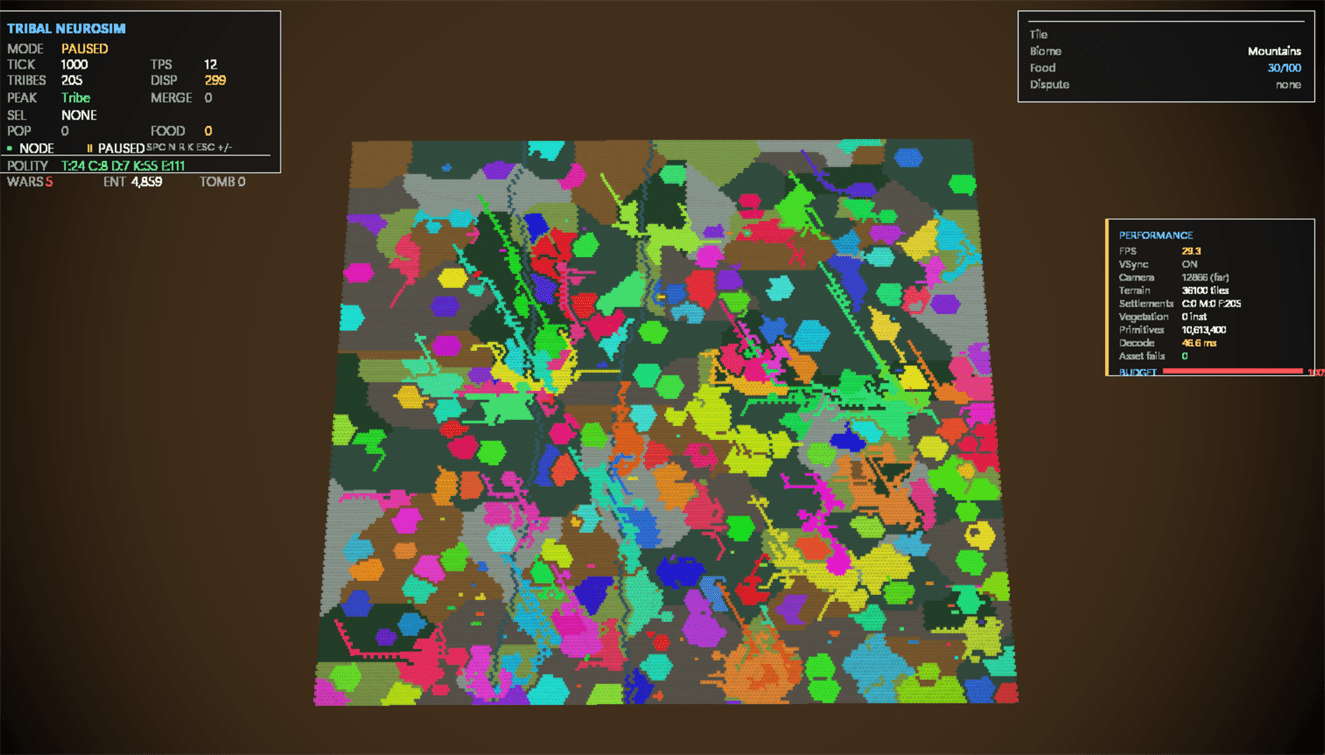
\includegraphics[width=0.9\textwidth]{assets/neurosim/run67fl7777-fl-s7777-tick1000.png}
\caption{Flexset, seed=7777, tick=1000: 205 élő törzs az F2 korai futtatással összevethető állapotban. Az összes polity-szint jelen van, a birodalom-korszak megkezdődött.}
\label{fig:neurosim-fl7777-tick1000}
\end{figure}

\begin{figure}[h]
\centering
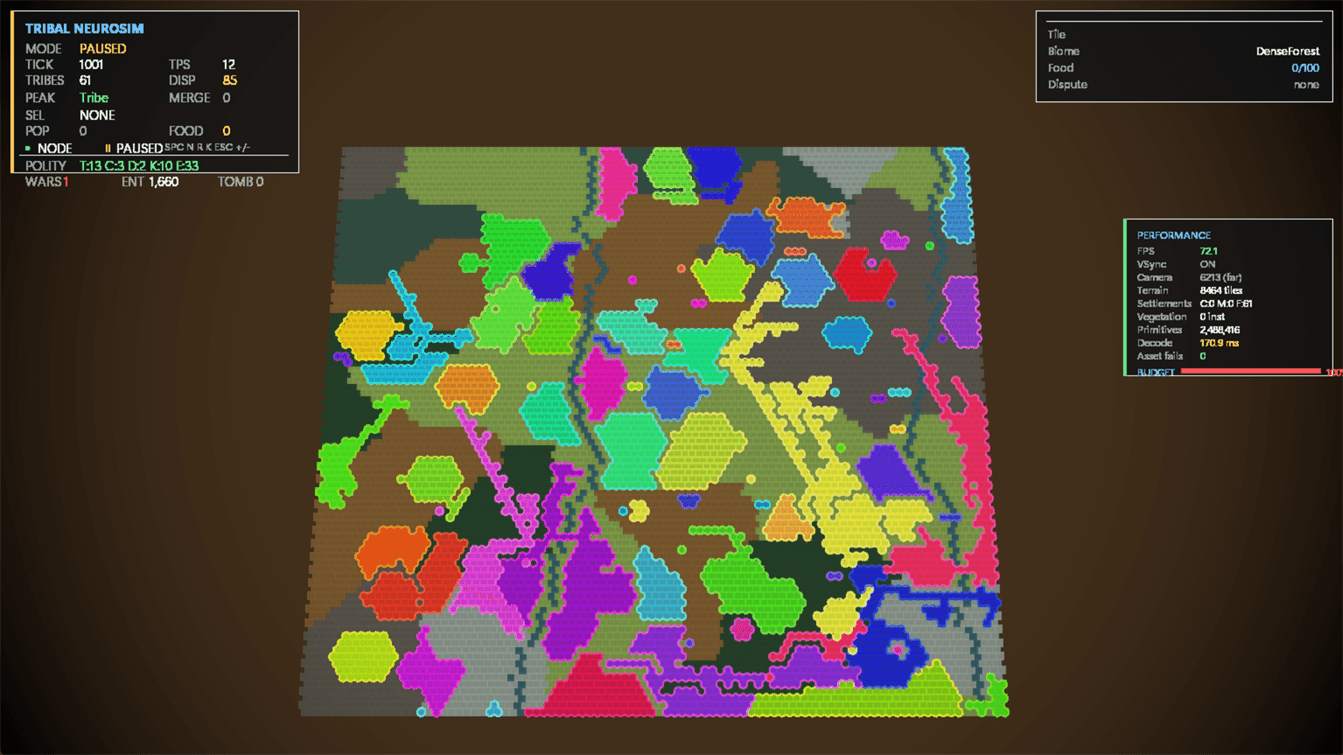
\includegraphics[width=0.9\textwidth]{assets/neurosim/run67sq7777-sq-s7777-tick1000.png}
\caption{SoloQ, seed=7777, tick=1000: 61 élő törzs, kisebb világ. Összehasonlításképpen: azonos tick-en a flexset futtatás 3,4$\times$ több entitást tartott életben - ez a két adatkészlet eltérő térbeli dinamikájának és kezdő törzsszámának közvetlen következménye.}
\label{fig:neurosim-sq7777-tick1000}
\end{figure}

% --------------------------------------------------------------------------
\subsection*{Javított determinisztikus futások}
% --------------------------------------------------------------------------

A 2026.~május~16-i post-first-run javítási kör után a validáció fókusza áthelyeződött:
nem az volt a kérdés, hogy a kimenetek aktívak-e, hanem az, hogy a teljes világ
visszaellenőrizhetően és determinisztikusan konvergál-e. Ebben a körben a kihalt törzsek
területe már öröklődött, az \texttt{AtWar} állapot nem okozott éhhalál-kaszkádot,
az artifact skálázás megszüntette a Warband-monokultúrát, és a tombstone rekordok
alapító PUUID szinten is auditálhatóbbá váltak.

A 2026.~május~18-i Tribe 397 futás már ezt a javított állapotot dokumentálta. A teljes,
599 törzses világ egyetlen túlélőig konvergált, és a végállapot nem csak képből, hanem
eseménysorból is rekonstruálható volt: Tribe 397 több védelmi győzelem, opportunista
háború és végső direkt konfliktus után maradt életben.

\begin{table}[h]
\centering
\caption{Javított determinisztikus futás kiemelt pontjai (Tribe 397, 2026-05-18).}
\label{tab:tribe397-validation}
\begin{tabular}{rlp{7.2cm}}
\hline
\textbf{Tick} & \textbf{Állapot} & \textbf{Értelmezés} \\
\hline
50   & 557 élő törzs & korai terjeszkedés, még birodalmak nélkül \\
900  & 277 élő törzs & erős konszolidáció, 105 Empire \\
5000--6900 & hosszú plateau & kevés, nagy birodalom tartja egymást nyomás alatt \\
7650 & 2 élő törzs & Tribe 397 és Tribe 269 végjáték \\
7800 & 1 élő törzs & Tribe 397 győztes, 51\,391 tile kontroll \\
\hline
\end{tabular}
\end{table}

\begin{lstlisting}[language={},caption={Javított végállapot-részlet a Tribe 397 futásból}]
[SIM tick=7800] alive=1 tiles=51391 max_tile=51391 avg_pop=5305532 wars_active=0
\end{lstlisting}

Ez a futás erősebb thesis-szintű bizonyíték, mint az F2: nem csak azt mutatja, hogy
a neurális hajtóerők aktívak, hanem azt is, hogy a javított szabályrendszer mellett
a teljes eseménysor auditálható, a végső győztes rekonstruálható, és a modell nem
ragad be szövetségi vagy békés deadlockba.

% --------------------------------------------------------------------------
\subsection*{Batch determinizmus-ellenőrzés}
% --------------------------------------------------------------------------

A determinizmus-javítás (lásd 22.4.~alszekció) helyességét batch futtatásokkal igazoltuk. A \texttt{run-batch.ps1} szkript képes $N$ párhuzamos fejnélküli futtatást azonos seed értékkel elindítani, és minden futtatás \texttt{final\_summary} rekordját JSON-ként rögzíteni. Az ellenőrzés feltétele: mind az $N$ rekordban azonos \texttt{TribeId} és azonos \texttt{PolityBehavior} értéknek kell szerepelnie.

Két batch-ellenőrzés elvégzése igazolta a javítás helyességét:

\textbf{Flexset, seed=42}: öt párhuzamos fejnélküli futtatás mindegyikében Tribe 596 (Warband/Combat viselkedési archetípus) győzött. A győztes \texttt{TribeId}, a \texttt{winner\_tier} és a \texttt{total\_ticks} értékek minden futtatásban bit-azonosak voltak.

\textbf{SoloQ, seed=7777}: a jelen fejezetben elemzett \texttt{run67sq7777} teljes futtatási logja szerint Tribe 70 győzött, tick=2541-nél. Ez a konkrét kísérleti narratíva ezért Tribe 70-et tekinti a seed=7777 SoloQ futtatás győztesének.

\begin{lstlisting}[language={}, caption={Batch determinizmus-ellenőrzés parancssora}]
# 5 futtatas azonos seed-del, eredmeny JSONL-be
.\run-batch.ps1 -Runs 5 -Seed 42 -DatasetId flexset
# Kimenet: final_summary sorok mind azonos winner_id-t es behavior-t mutatnak
\end{lstlisting}

Ez az eredmény két dolgot igazol egyszerre: egyrészt hogy a \texttt{clusters.sort\_by} javítás valóban megszüntette a véletlenszerű klasztersorrendből fakadó divergenciát, másrészt hogy a neurális hálózat és a szimulációs motor együttes viselkedése determinisztikus a teljes futtatás hosszán keresztül - nemcsak az első 100 tickre, amelyet a MonoGame-CLI összehasonlítás igazolt.

% --------------------------------------------------------------------------
\subsection*{Mit támogat a validáció - és mit nem}
% --------------------------------------------------------------------------

\textbf{A validáció alátámasztja az alábbi állításokat:}

\begin{itemize}
  \item A klaszter-derivált priorok mérhetően eltérő szimulált viselkedést produkálnak különböző adatkészletek esetén.
  \item A Flexset inicializáció mindkét tesztelt seednél konvergens viselkedési kimenetelhez vezet (Warband/Combat archetípus, alacsony agresszió, magas migráció).
  \item A SoloQ inicializáció seedenként változékony viselkedési kimenetelt produkál.
  \item A futtatások reprodukálhatók: azonos seed és adatkészlet esetén a győztes és a teljes final\_summary rekord bit-azonos marad.
  \item A törzsi viselkedés esemény-naplókkal alátámasztható: minden állítás (kaszkádháborúk, trilaterális koalíciók, sorozatos védelmi győzelmek) konkrét JSONL-bejegyzésekre hivatkozik.
\end{itemize}

\textbf{A validáció nem bizonyítja az alábbiakat:}

\begin{itemize}
  \item Hogy a modell valóság-konform - a szimulációs szabályok közelítések, nem valódi emberi viselkedés leírásai.
  \item Hogy az eredmények átvihetők tényleges LoL-meccs kimenetelekre vagy valódi csapatdinamikára.
  \item Hogy a győztes viselkedési archetípus objektíven a legjobb stratégia - csupán annyi igaz, hogy a választott szabályok alatt, ebben a szimulációs környezetben nyert.
  \item Hogy a Flexset és SoloQ klaszterprofilok közötti különbség \textit{oka} a megfigyelt viselkedési divergenciának - a kapcsolat korrelatív, nem okozati.
\end{itemize}

Ez a határ nem gyengíti a kísérlet eredményét, hanem pontosítja a thesis-érvényes állítások körét: a Tribal NeuroSim demonstrálja, hogy gráf-derivált klaszterprofilok mérhetően eltérő emergáló dinamikát indítanak el azonos szabálykörnyezetben. Ez a demonstráció reprodukálható, inspektálható és esemény-alapon igazolt.

% ==========================================================================
\section{Kísérleti futtatási narratívák}
\label{sec:neurosim-26-runs}
% ==========================================================================

Ez a szekció a négy teljes kísérleti futtatást esemény-narratívaként mutatja be. A cél nem az, hogy a térképképeket önmagukban bizonyítékként kezelje, hanem hogy a futtatási naplókból származó tick-számokat, háborús eseményeket és végállapotokat értelmezhető kísérleti történetté rendezze. A konfliktusos szerkezetek értelmezésekor a 23.4.~alszekció táblázatában bevezetett típusokra hivatkozom vissza: a tömeges opportunista háborúk, a többfrontos nyomás és a végjátékbeli párharcok ugyanannak az eseménybusz-alapú mechanikának különböző megfigyelhető formái.

\subsection*{Flexset, seed=7777}

\begin{table}[h]
\centering
\caption{Flexset seed=7777 futtatás összefoglalója}
\label{tab:neurosim-run-fl7777-summary}
\begin{tabular}{ll}
\hline
\textbf{Mező} & \textbf{Érték} \\
\hline
Adatkészlet & flexset (EUNE Master+ Flex Queue) \\
Seed & 7777 \\
Indítótörzsek & 599 \\
Térkép & $\approx$36\,100 tile \\
Végső tick & 2538 \\
Győztes & Tribe 355 \\
Behavior / fókusz & Empire / Warband / Combat \\
Agresszió & 0,18 \\
Migráció & 0,88 \\
Kulcsesemény & Totális Háború, tick=2040: 64 egyidejű deklaráció \\
\hline
\end{tabular}
\end{table}

A flexset seed=7777 futtatás 599, Flex Queue klaszterprofilból inicializált törzzsel indult egy $\approx$36\,100 tile-os térképen, és tick=2538-nál ért véget. A győztes, Tribe 355, Empire / Warband / Combat archetípusú entitás volt, 0,18-as agresszióval, 0,88-as migrációval és 0,98-as A\_combat értékkel. Ez a profil már az első flexset narratívában megmutatja a később visszatérő mintát: nem a magas nyers agresszió, hanem a magas harci kompetencia, a területi mobilitás és az opportunista, de fegyelmezett háborúindítás vezetett győzelemhez.

Az első szakasz gyors, de még nem dominancia-jellegű proliferáció volt. Tick=50-nél mind az 599 törzs élt, tick=150-nél 562 maradt, és az első \textit{SURROUNDED} esemény tick=150-nél jelent meg. Az első Empire tick=264-nél Tribe 372 volt: Pathfinders / MapObjective viselkedésű, 15\,820 populációval, 50 tile-lal, 0,35-ös fitnesszel és 0,88-as migrációs hajtóerővel. Mivel ekkor még 516 törzs élt, ez az első birodalom nem hegemóniát, hanem korai fejlődési küszöbátlépést jelentett.

A középső konszolidációt a védelmi túlélés és az abszorpciós háborúk uralták. Tick=900-nál még 310 törzs élt, majd tick=900 és tick=950 között 85 törzs esett ki 50 tick alatt; ez a futtatás leggyorsabb kihalási pulzusa volt. Tick=1000-re 205 túlélő maradt, átlagosan 28\,232 populációval. Tribe 355 ebben a szakaszban nem front-runnerként jelent meg: a napló szerint tick=1155-nél támadta és győzte le Tribe 353-at, majd később több támadót is visszavert, köztük Tribe 281-et tick=1458-nál, Tribe 480-at tick=1600-nál, Tribe 504-et tick=1859-nél és Tribe 530-at tick=1920-nál.

A 23.4.~alszekcióban tárgyalt tömeges opportunista konfliktustípus legtisztább példája tick=2040-nél következett be: 64 opportunity war deklaráció indult egyetlen tick alatt. Tick=2043-nál 68 túlélő és 32 aktív háború látható, minden releváns szereplő Empire-szinten. A kaszkád tick=2050-nél 63, tick=2100-nál 43, tick=2150-nél 33, tick=2200-nál 20, tick=2250-nél pedig már csak 13 túlélőt hagyott. Tágabb nézetben a tick=1000-es 205 túlélőből az empire-korszak végére 13 maradt; a közvetlen Totális Háború ablaka viszont tick=2043 és tick=2250 között sűrítette le a mezőnyt 68-ról 13-ra.

A végjáték tick=2497-nél két szereplőre szűkült: Tribe 355 és Tribe 470. Tribe 355 ekkor 21\,751 tile-t, 2\,510\,325 populációt, 0,63-as fitneszt, 0,98-as A\_combatot és 0,83-as raid drive-ot tartott; Tribe 470 Pathfinders / MapObjective profilként 7\,956 tile-on és 1\,848\,421 populációval állt szemben vele. A térképi arány ekkor már eldőlt: Tribe 355 közel háromszoros területelőnyben volt. Tick=2520-nál raid-opportunity jelent meg Tribe 470 ellen, majd tick=2538-nál Tribe 355 támadott és győzött. A végállapotban 1\,187\,885 populációt, 3\,504\,309 food tartalékot és 37\,666 tile-t tartott.

\begin{figure}[h]
\centering
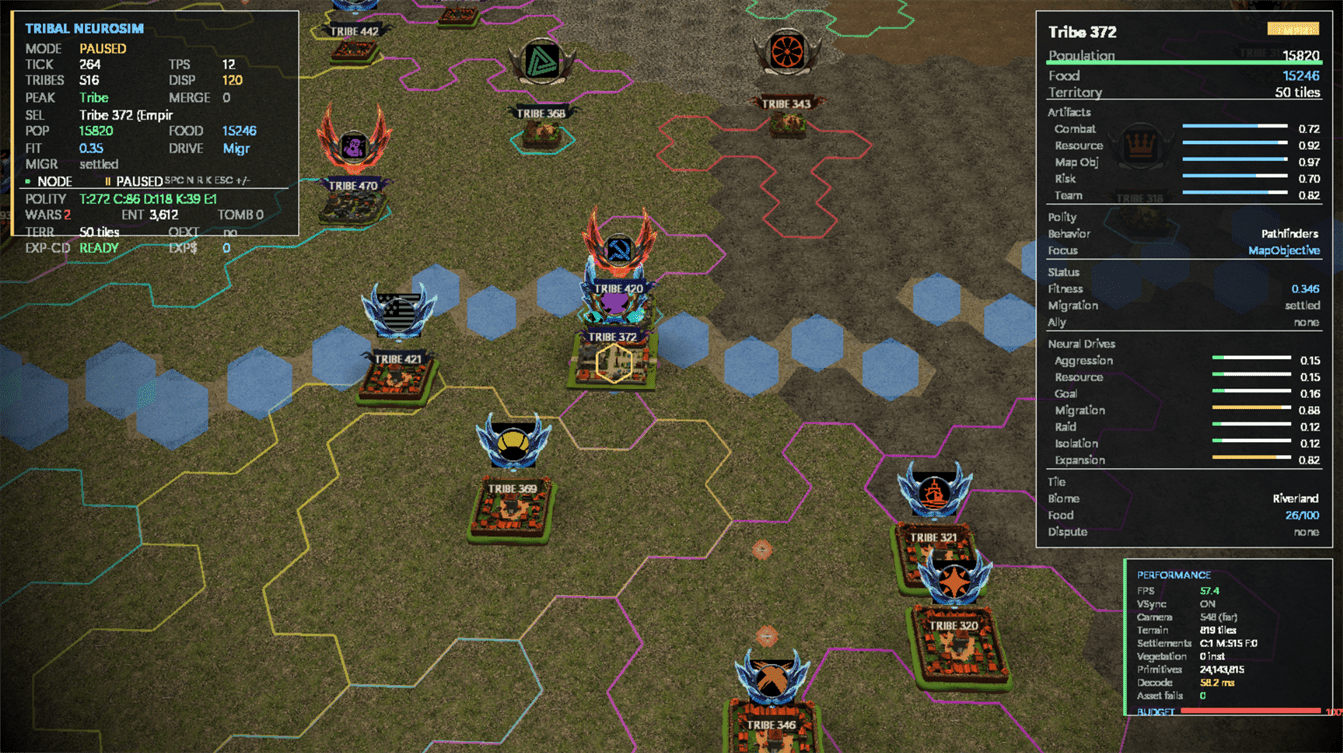
\includegraphics[width=0.9\textwidth]{assets/neurosim/run67fl7777-fl-s7777-tick264-firstempire.png}
\caption{Flexset, seed=7777, tick=264: az első Empire, Tribe 372, Pathfinders / MapObjective profillal.}
\label{fig:neurosim-run-fl7777-firstempire}
\end{figure}

\begin{figure}[h]
\centering
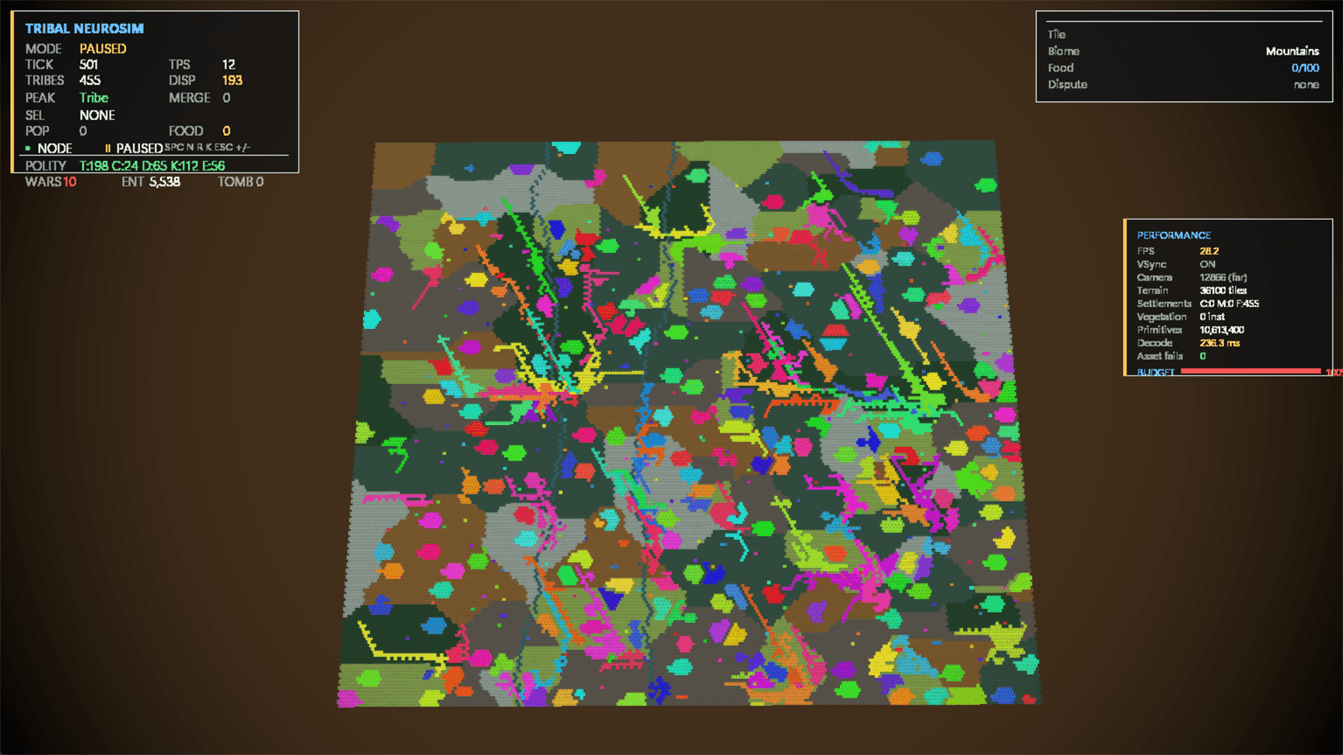
\includegraphics[width=0.9\textwidth]{assets/neurosim/run67fl7777-fl-s7777-tick500.png}
\caption{Flexset, seed=7777, tick=500: középső konszolidációs állapot, még sok kis- és középszintű entitással.}
\label{fig:neurosim-run-fl7777-tick500}
\end{figure}

\begin{figure}[h]
\centering
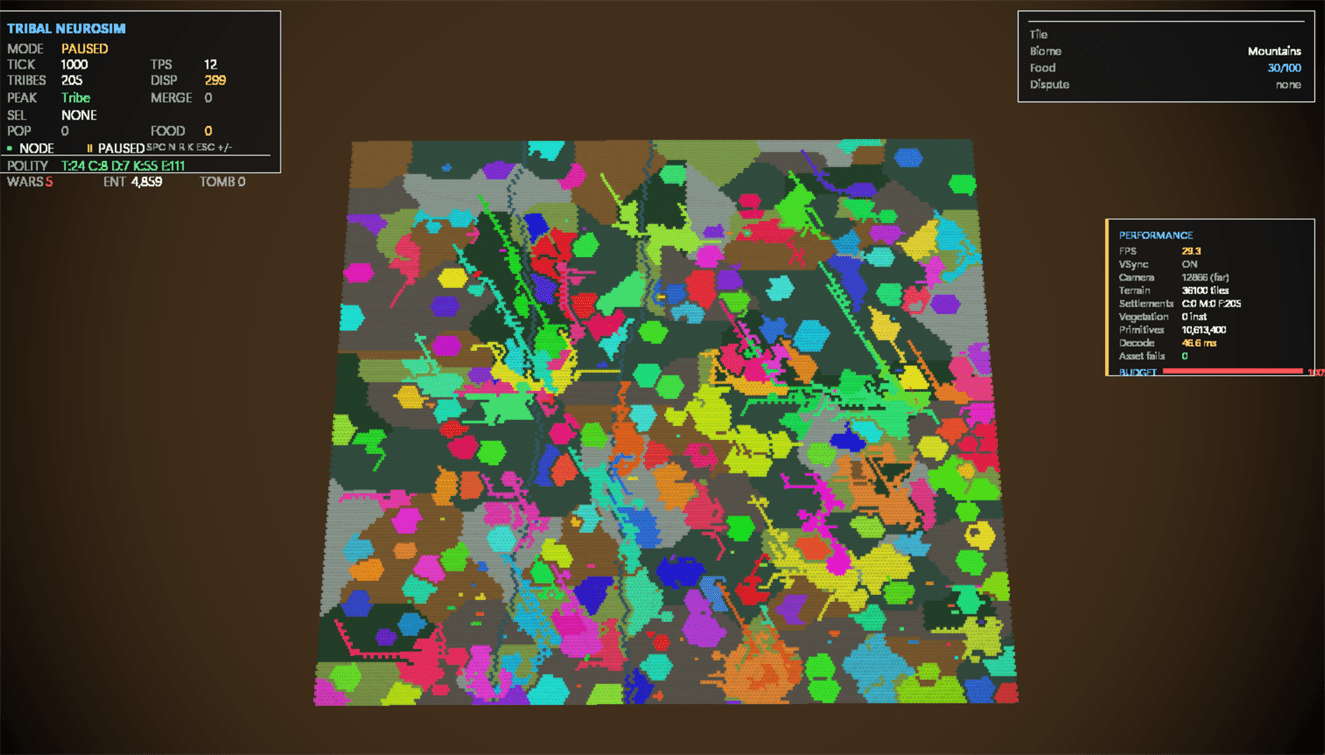
\includegraphics[width=0.9\textwidth]{assets/neurosim/run67fl7777-fl-s7777-tick1000.png}
\caption{Flexset, seed=7777, tick=1000: 205 túlélő; az Empire-korszak érdemben megkezdődött.}
\label{fig:neurosim-run-fl7777-tick1000}
\end{figure}

\begin{figure}[h]
\centering
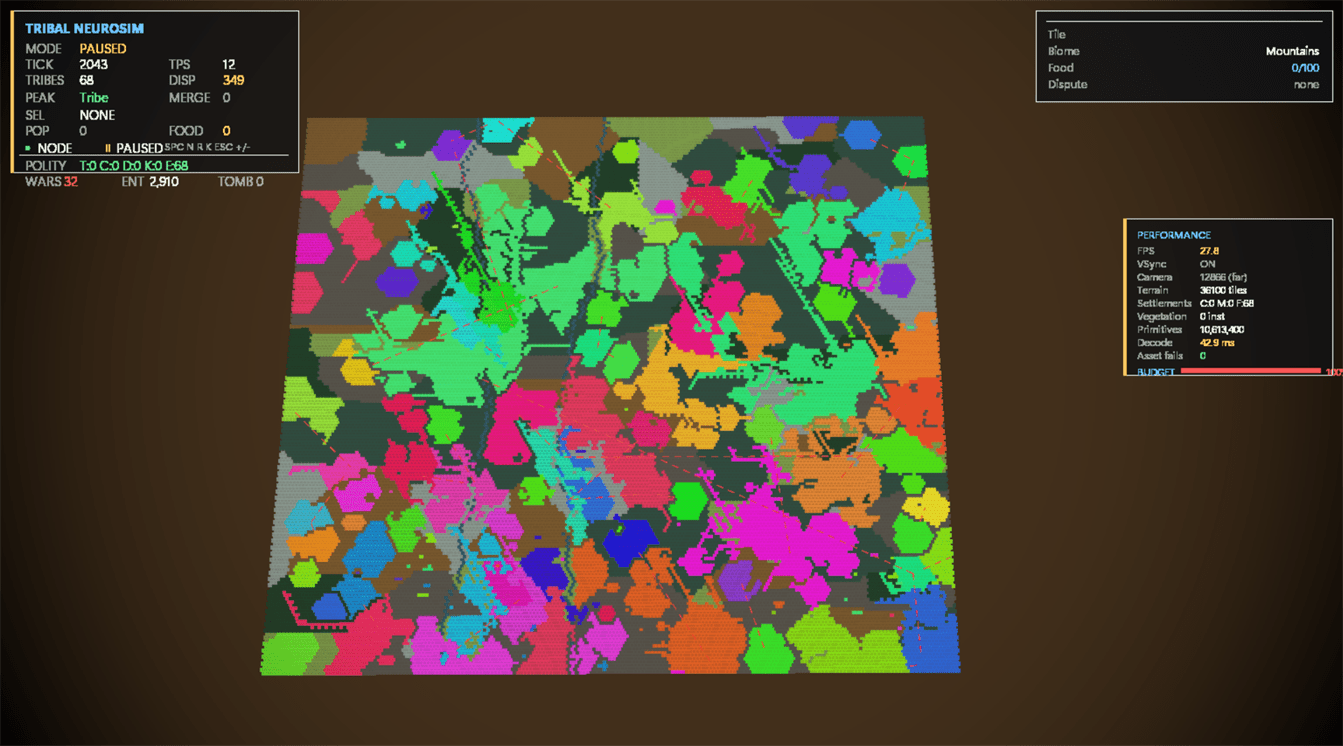
\includegraphics[width=0.9\textwidth]{assets/neurosim/run67fl7777-fl-s7777-tick2043-totalwar.png}
\caption{Flexset, seed=7777, tick=2043: a tick=2040-es Totális Háború utáni állapot, 68 túlélővel és 32 aktív háborúval.}
\label{fig:neurosim-run-fl7777-totalwar}
\end{figure}

\begin{figure}[h]
\centering
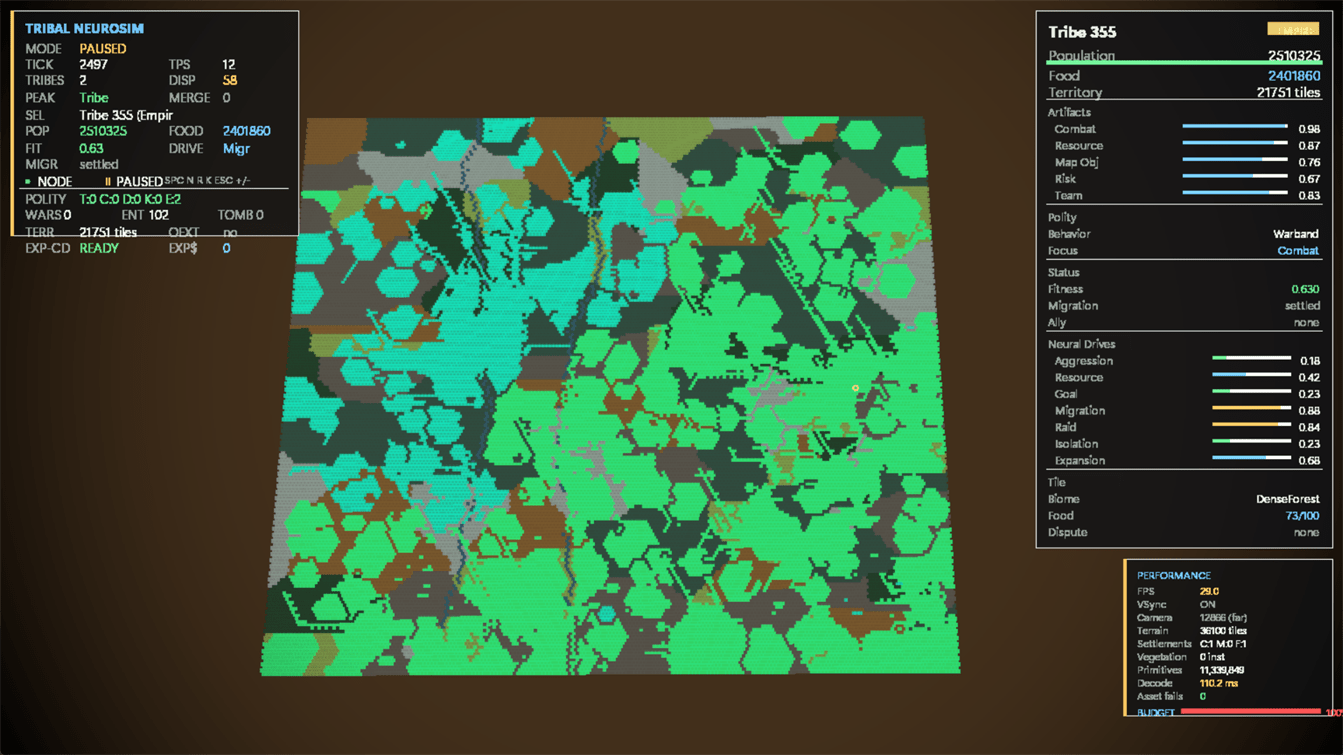
\includegraphics[width=0.9\textwidth]{assets/neurosim/run67fl7777-fl-s7777-tick2497-last2A.png}
\caption{Flexset, seed=7777, tick=2497: végső két szereplő, Tribe 355 profilja.}
\label{fig:neurosim-run-fl7777-last2a}
\end{figure}

\begin{figure}[h]
\centering
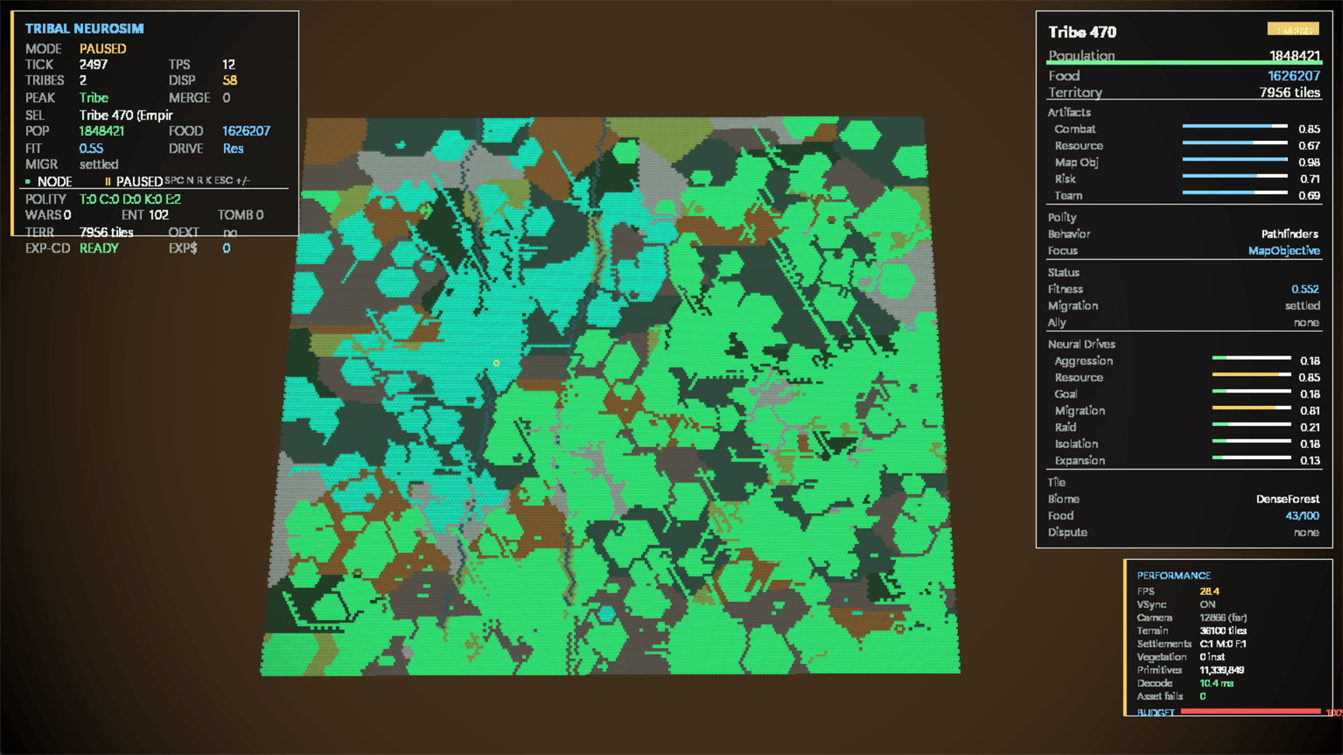
\includegraphics[width=0.9\textwidth]{assets/neurosim/run67fl7777-fl-s7777-tick2497-last2B.png}
\caption{Flexset, seed=7777, tick=2497: végső két szereplő, Tribe 470 profilja.}
\label{fig:neurosim-run-fl7777-last2b}
\end{figure}

\begin{figure}[h]
\centering
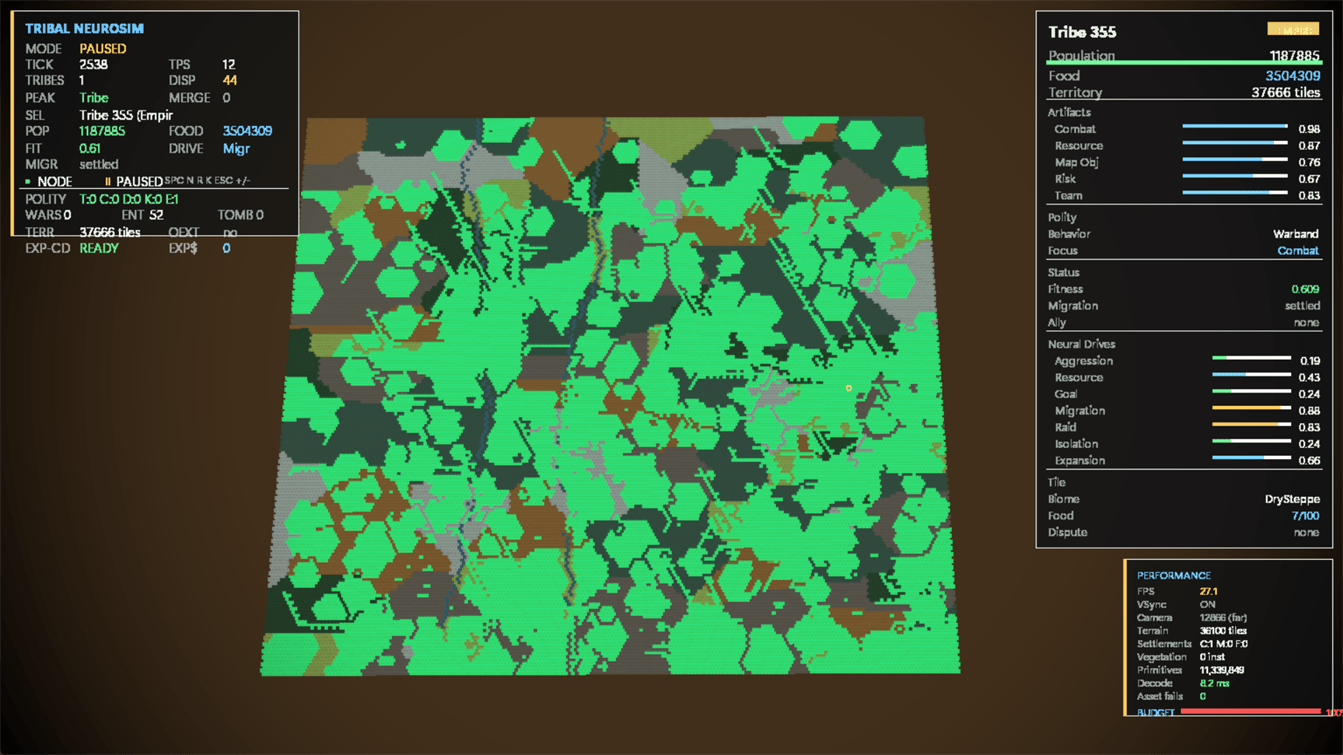
\includegraphics[width=0.9\textwidth]{assets/neurosim/run67fl7777-fl-s7777-tick2538-last.png}
\caption{Flexset, seed=7777, tick=2538: Tribe 355 győzelme, 37\,666 tile-os végső területtel.}
\label{fig:neurosim-run-fl7777-last}
\end{figure}

\subsection*{Flexset, seed=42}

\begin{table}[h]
\centering
\caption{Flexset seed=42 futtatás összefoglalója}
\label{tab:neurosim-run-fl42-summary}
\begin{tabular}{ll}
\hline
\textbf{Mező} & \textbf{Érték} \\
\hline
Adatkészlet & flexset (EUNE Master+ Flex Queue) \\
Seed & 42 \\
Indítótörzsek & 599 \\
Térkép & $\approx$36\,100 tile \\
Végső tick & 2487 \\
Győztes & Tribe 596 \\
Behavior / fókusz & Empire / Warband / Combat \\
Agresszió & 0,13 \\
Migráció & 0,87 \\
Kulcsesemény & Tick=2400 trilaterális háború Tribe 557 ellen \\
\hline
\end{tabular}
\end{table}

A flexset seed=42 futtatás ugyanazzal a 599 törzses Flex Queue inicializációs nagyságrenddel és $\approx$36\,100 tile-os térképpel indult, mint a seed=7777 változat, de a végjáték szerkezete eltért. A győztes Tribe 596 lett, szintén Empire / Warband / Combat profillal, 0,13-as agresszióval, 0,87-es migrációval és 0,96-os A\_combat értékkel. A két flexset futtatás közös tanulsága ezért erős: eltérő seed mellett is alacsony agressziójú, magas migrációjú, harci fókuszú Warband nyert.

A korai szakasz tick=287-nél hozta az első Empire-t. Tribe 220 Council / Team viselkedésű entitásként jelent meg, 15\,737 populációval, 68 tile-lal és 0,38-as fitnesszel. Ez különösen figyelemre méltó, mert a későbbi flexset győztesek Warband / Combat profilok voltak; az első fejlett polity itt kooperatív Council típus volt, nem a végül győztes archetípus előképe. Tick=500-nál Tribe 244 Warband / Combat entitásként 41\,042 populációt és 89 tile-t tartott, miközben 443 törzs még életben volt.

A középső szakaszban a seed=42 futtatás lassabban lépett át a teljes Empire-korszakba, mint a seed=7777, de a tick=900 és tick=950 közötti 64 kiesés itt is mass extinction burstként értelmezhető. Tick=1000-nél 234 túlélő volt, ebből 117 Empire. Tribe 596 ebben a fázisban nem domináns térképi szereplőként, hanem kitartó védőként építette fel harci értékét: a napló szerint Tribe 520 tick=300 körül, Tribe 521 tick=823-nál, majd Tribe 571 tick=939-nél támadta, és mindegyik támadó vereséget szenvedett.

A tömeges háborús fázis tick=1860-nál indult: 72 opportunity war deklaráció történt egyetlen tick alatt, ami nagyobb abszolút burst volt, mint a seed=7777 64 deklarációs Totális Háborúja. Tick=1872-nél 67 túlélő és 26 aktív háború látszott; 63 entitás már Empire-szintű volt. A 23.4.~alszekció konfliktusos struktúrái közül ez a futtatás előbb a tömeges opportunista kaszkádot, majd később a többfrontos, trilaterális nyomást mutatja be.

A döntő esemény tick=2400-nál következett be. Ekkor Tribe 90 és Tribe 596 egymástól függetlenül, ugyanabban a tickben támadta meg a domináns Tribe 557-et, amely a tick=2352-es Tribe 435 elleni győzelme után körülbelül 23\,149 tile-ra nőtt. A naplózott deklarációk szerint Tribe 90 agressziója 0,84, Tribe 596 agressziója 0,14 volt; vagyis ugyanaz a célpont két nagyon eltérő viselkedési profilból vált támadhatóvá. Tick=2417-nél a háromszereplős állapot még fennállt, majd tick=2424-nél Tribe 596 legyőzte Tribe 557-et, felszívta annak területét, és több mint 28\,000 tile-ra nőtt.

A végső párharc Tribe 90 és Tribe 596 között zajlott. Tick=2486-nál Tribe 90 Pathfinders / MapObjective profilként 11\,207 tile-on, 19\,366 populációval és 0,84-es agresszióval állt, míg Tribe 596 Warband / Combat profilként 28\,162 tile-t, 233\,960 populációt és 0,13-as agressziót tartott. Tribe 90 map-objective és risk értékei magasabbak voltak, de a trilaterális háborúban elvesztette populációs tartalékát. Tick=2487-nél Tribe 596 legyőzte Tribe 90-et, 329\,859 populációval, 2\,738\,854 food tartalékkal és 39\,369 tile-os végső területtel zárva a futtatást.

\begin{figure}[h]
\centering
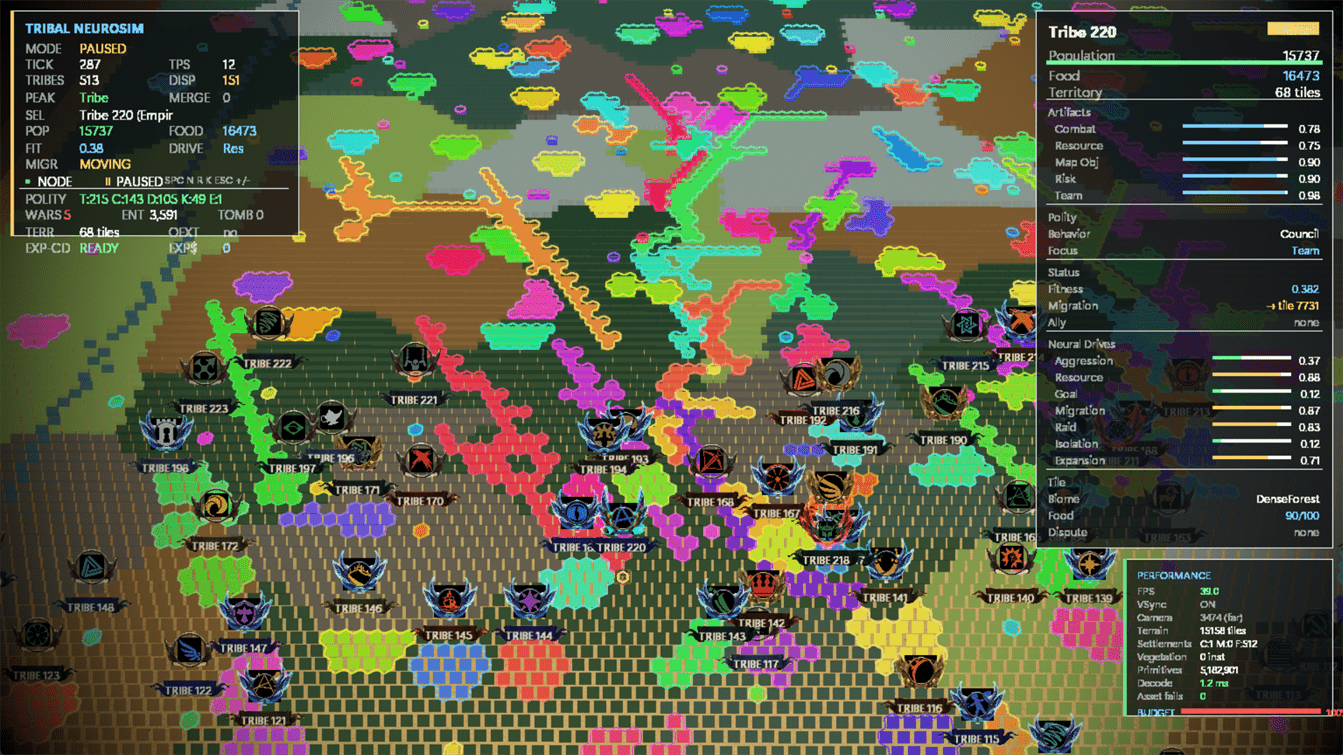
\includegraphics[width=0.9\textwidth]{assets/neurosim/run67fl42-fl-s42-tick287-firstempire.png}
\caption{Flexset, seed=42, tick=287: az első Empire, Tribe 220, Council / Team profillal.}
\label{fig:neurosim-run-fl42-firstempire}
\end{figure}

\begin{figure}[h]
\centering
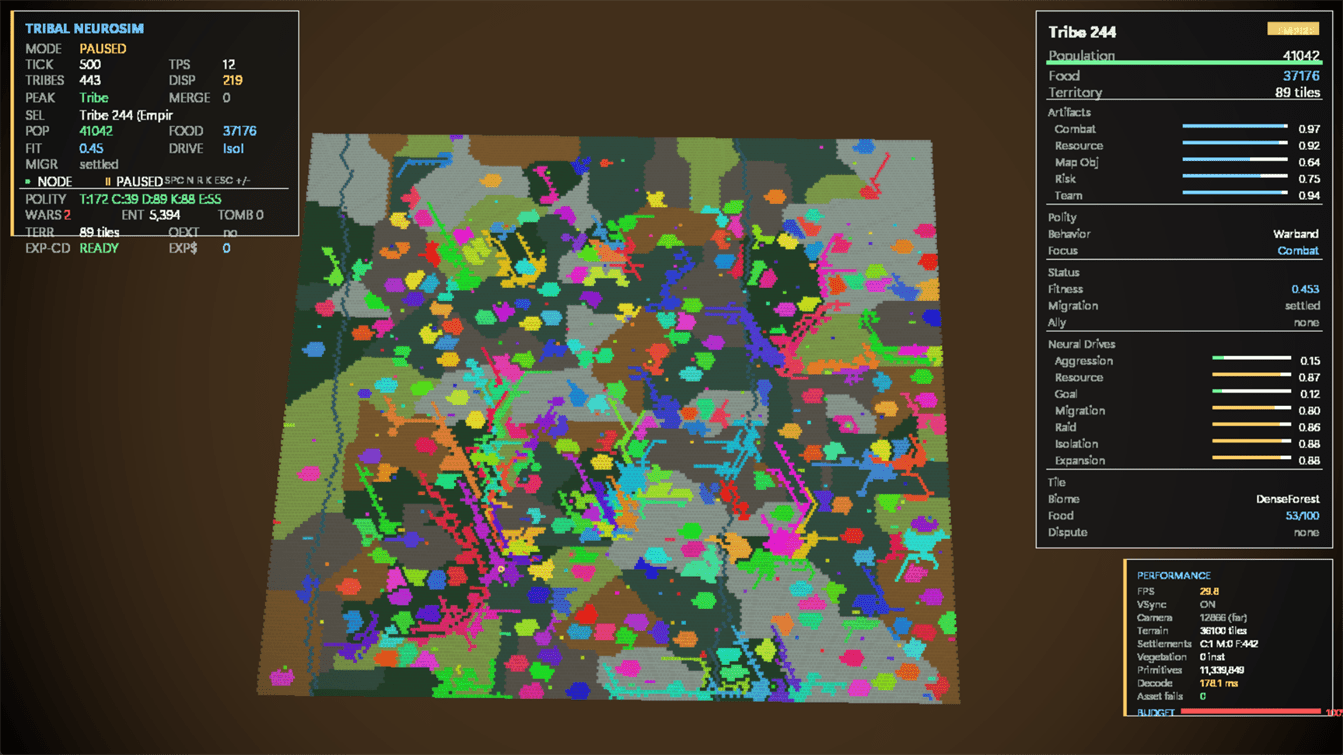
\includegraphics[width=0.9\textwidth]{assets/neurosim/run67fl42-fl-s42-tick500.png}
\caption{Flexset, seed=42, tick=500: középső konszolidáció, Tribe 244 kiemelt Warband / Combat profillal.}
\label{fig:neurosim-run-fl42-tick500}
\end{figure}

\begin{figure}[h]
\centering
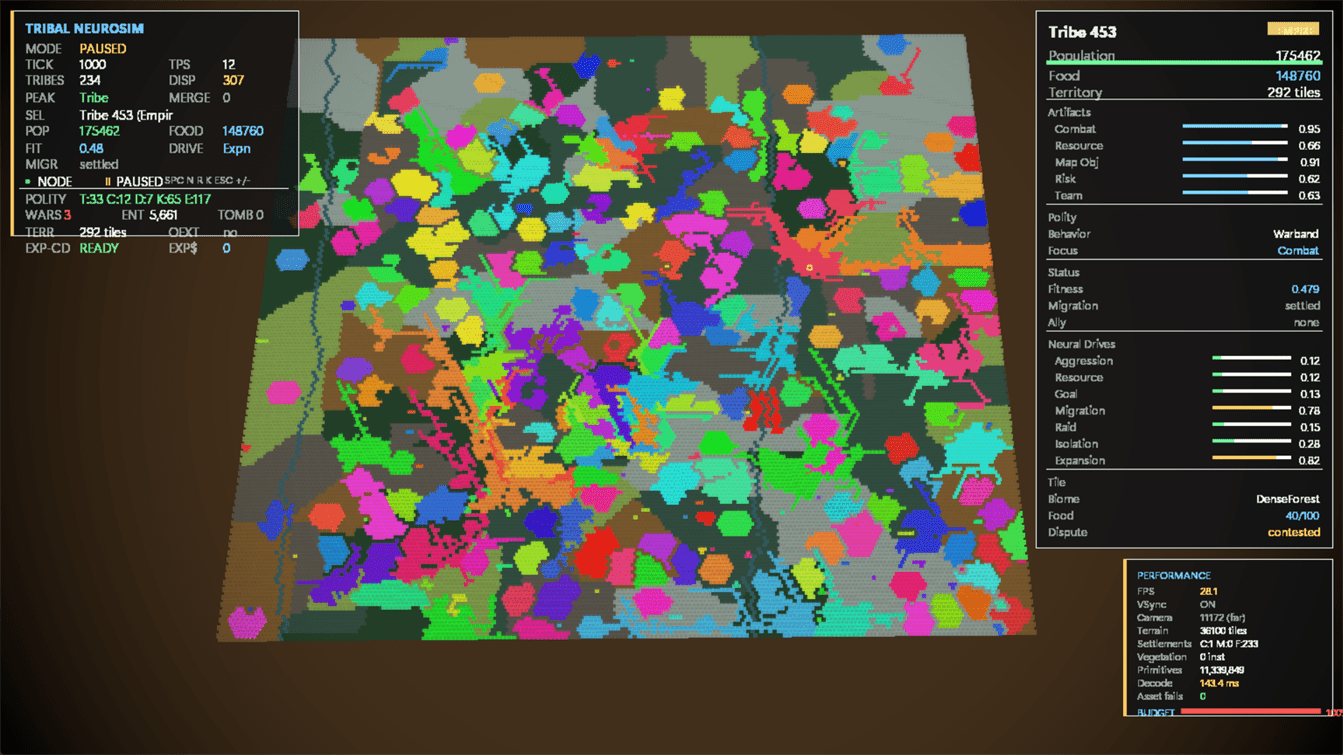
\includegraphics[width=0.9\textwidth]{assets/neurosim/run67fl42-fl-s42-tick1000.png}
\caption{Flexset, seed=42, tick=1000: Empire-korszak, 234 túlélővel.}
\label{fig:neurosim-run-fl42-tick1000}
\end{figure}

\begin{figure}[h]
\centering
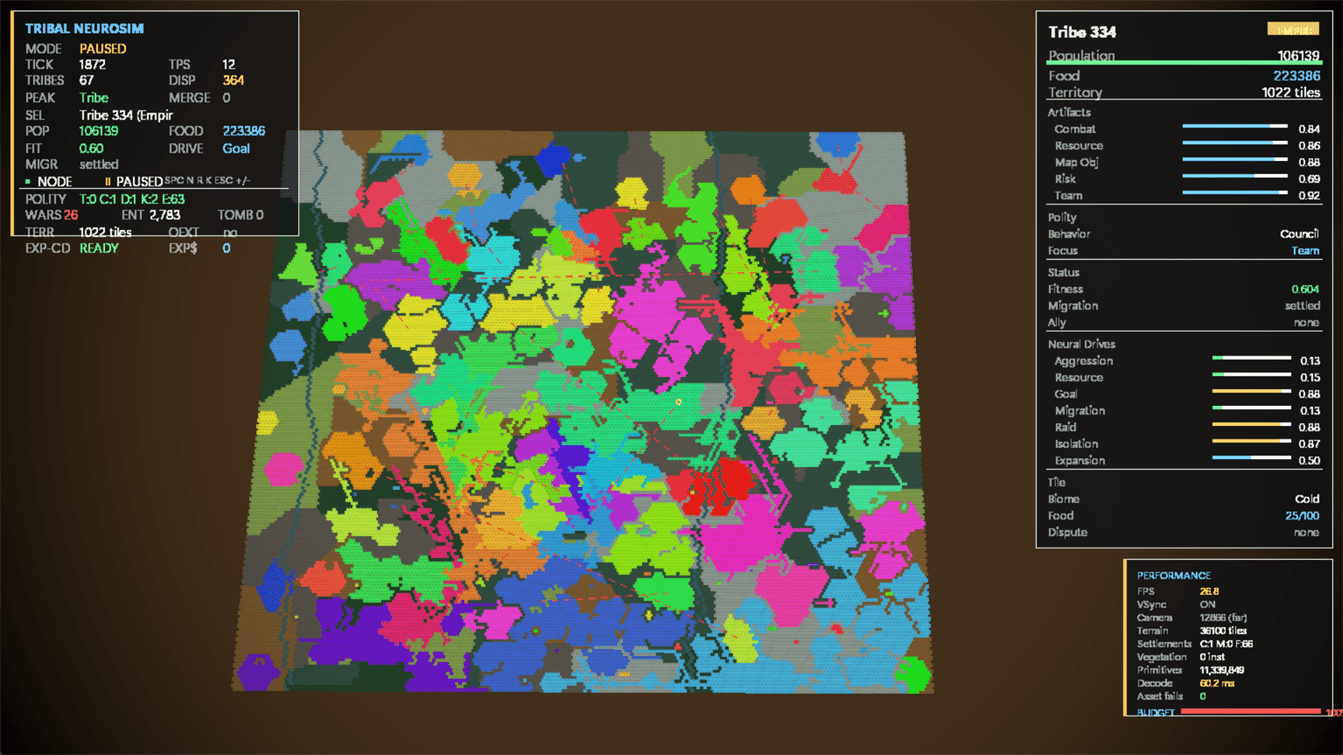
\includegraphics[width=0.9\textwidth]{assets/neurosim/run67fl42-fl-s42-tick1872-totalwar.png}
\caption{Flexset, seed=42, tick=1872: a tick=1860-as, 72 deklarációs Total War utáni állapot.}
\label{fig:neurosim-run-fl42-totalwar}
\end{figure}

\begin{figure}[h]
\centering
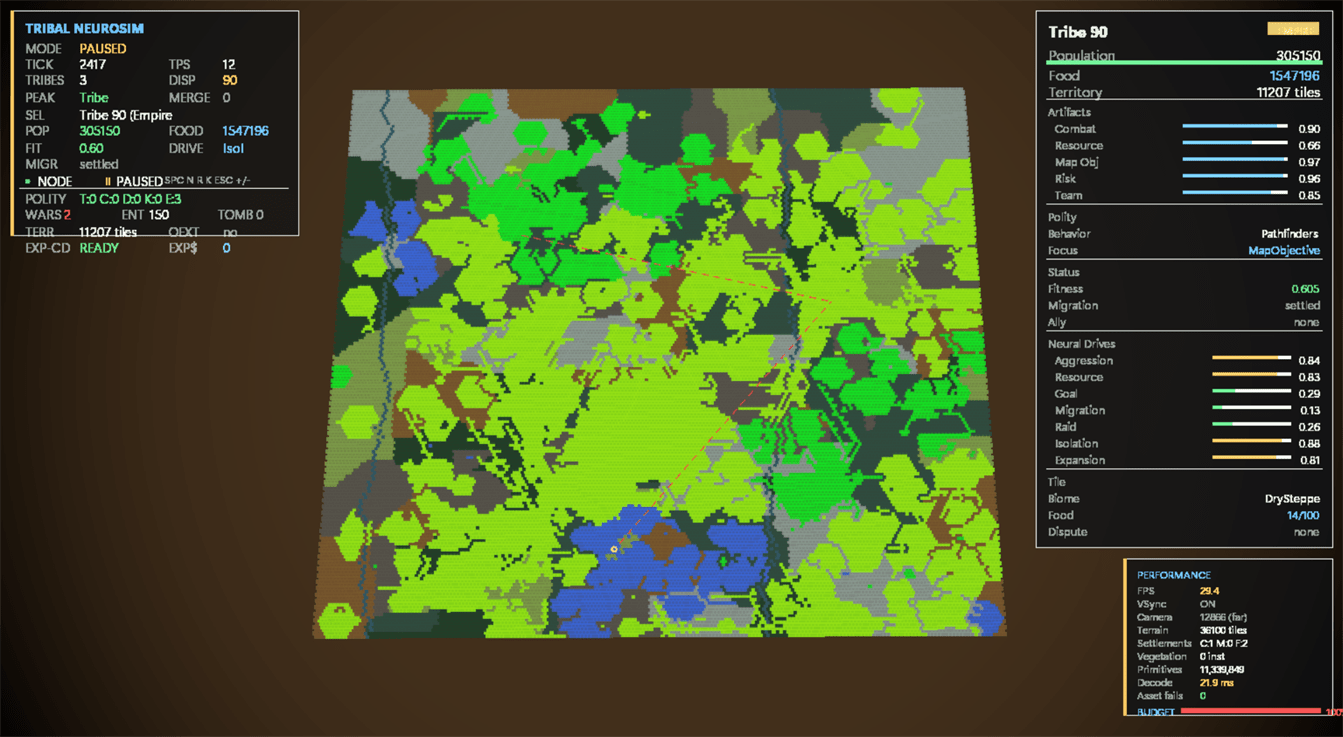
\includegraphics[width=0.9\textwidth]{assets/neurosim/run67fl42-fl-s42-tick2417-trilateralwar.png}
\caption{Flexset, seed=42, tick=2417: trilaterális háború Tribe 90, Tribe 596 és a domináns Tribe 557 között.}
\label{fig:neurosim-run-fl42-trilateralwar}
\end{figure}

\begin{figure}[h]
\centering
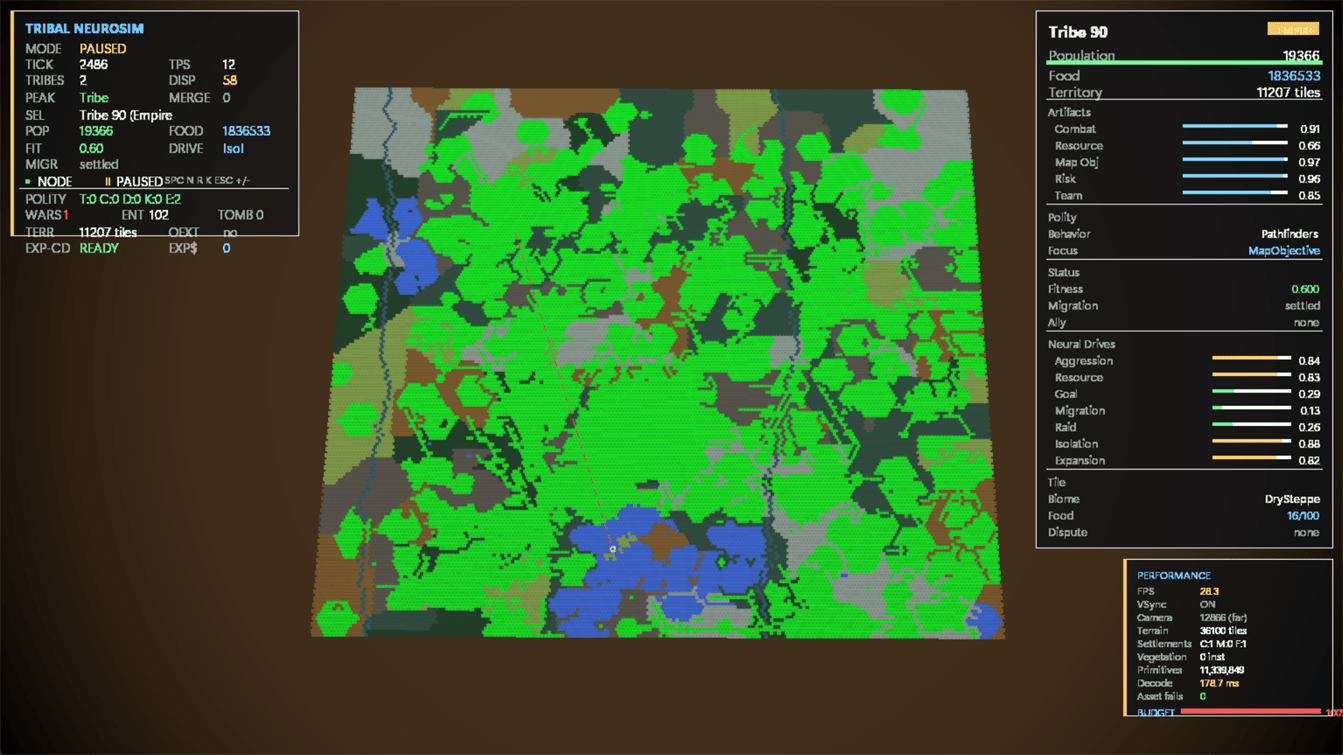
\includegraphics[width=0.9\textwidth]{assets/neurosim/run67fl42-fl-s42-tick2486-last2A.png}
\caption{Flexset, seed=42, tick=2486: végső két szereplő, Tribe 90 profilja.}
\label{fig:neurosim-run-fl42-last2a}
\end{figure}

\begin{figure}[h]
\centering
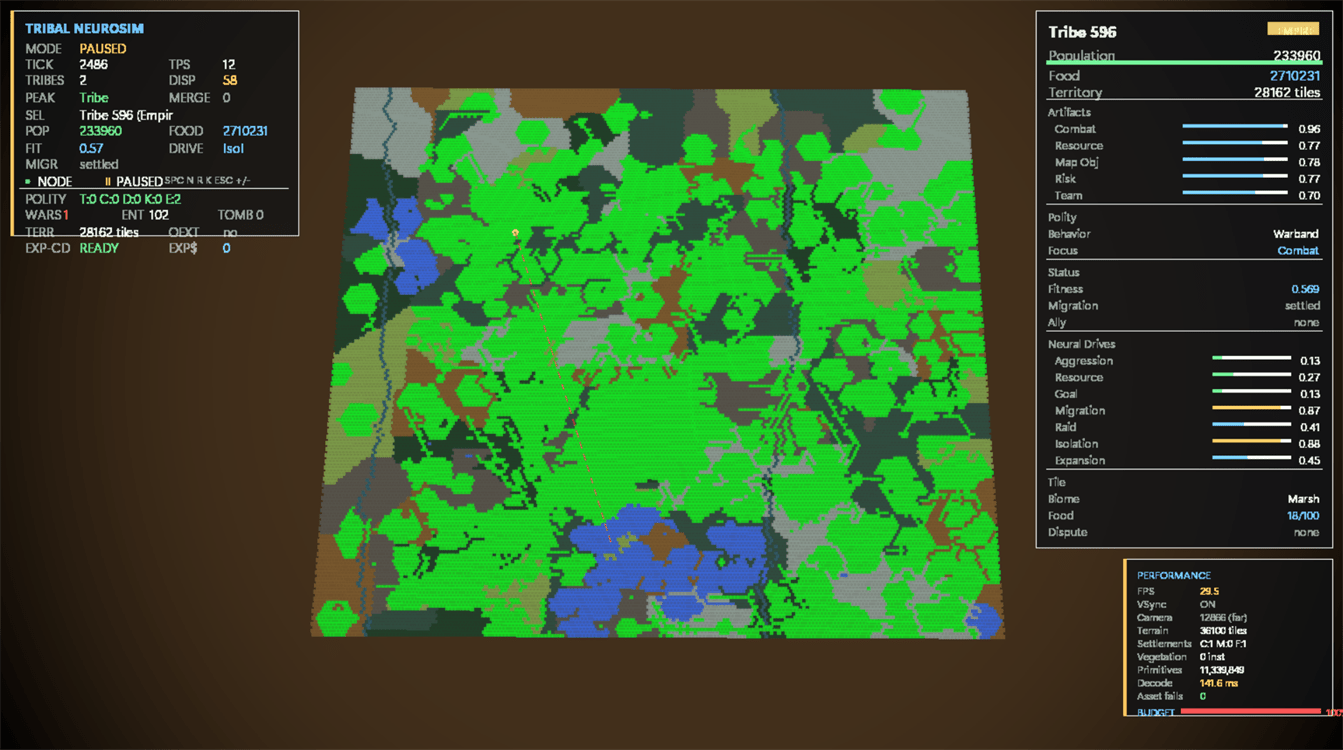
\includegraphics[width=0.9\textwidth]{assets/neurosim/run67fl42-fl-s42-tick2486-last2B.png}
\caption{Flexset, seed=42, tick=2486: végső két szereplő, Tribe 596 profilja.}
\label{fig:neurosim-run-fl42-last2b}
\end{figure}

\begin{figure}[h]
\centering
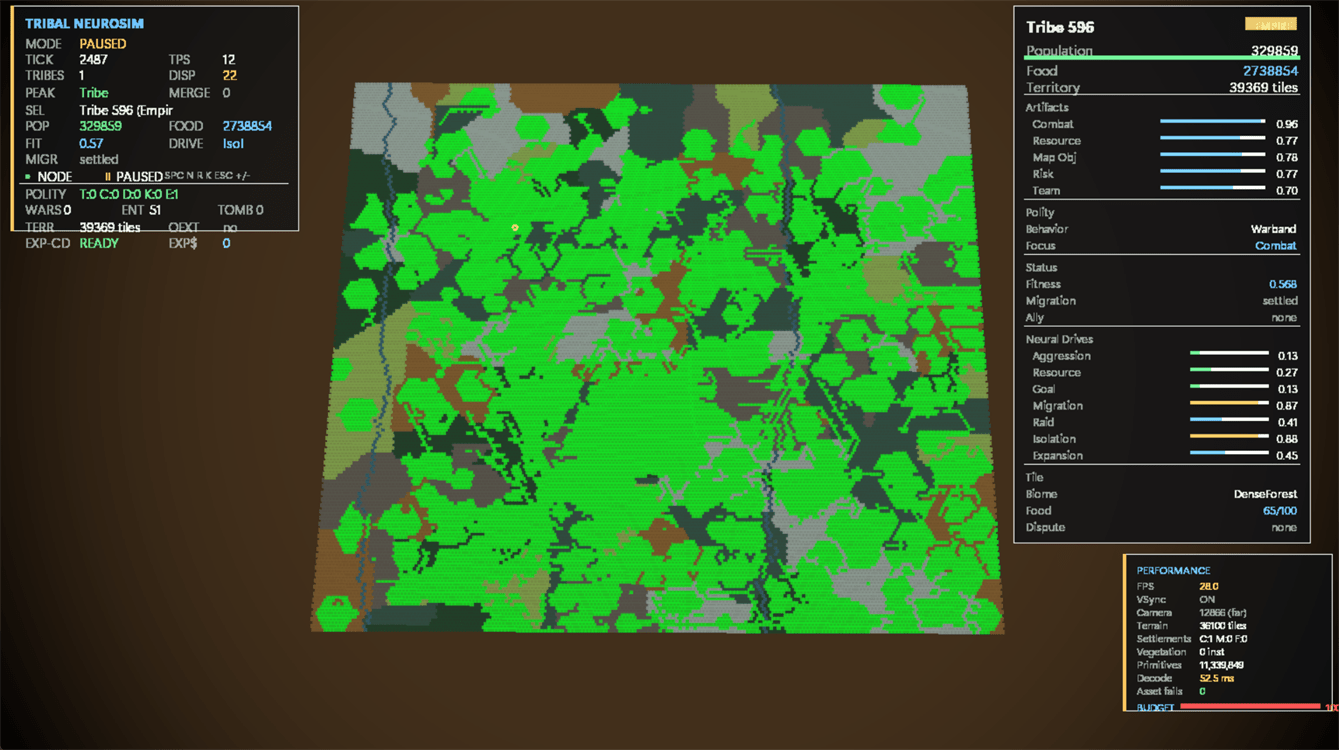
\includegraphics[width=0.9\textwidth]{assets/neurosim/run67fl42-fl-s42-tick2487-last.png}
\caption{Flexset, seed=42, tick=2487: Tribe 596 győzelme, 39\,369 tile-os végső területtel.}
\label{fig:neurosim-run-fl42-last}
\end{figure}

\subsection*{SoloQ, seed=42}

\begin{table}[h]
\centering
\caption{SoloQ seed=42 futtatás összefoglalója}
\label{tab:neurosim-run-sq42-summary}
\begin{tabular}{ll}
\hline
\textbf{Mező} & \textbf{Érték} \\
\hline
Adatkészlet & soloq (EUNE Master+ Solo Queue) \\
Seed & 42 \\
Indítótörzsek & 140 \\
Térkép & végső győztes terület: 6\,356 tile \\
Végső tick & 2046, a leggyorsabb futtatás \\
Győztes & Tribe 89 \\
Behavior / fókusz & Empire / Vanguard / Risk \\
Agresszió & 0,13 \\
Migráció / raid / izoláció & 0,16 / 0,14 / 0,88 \\
Kulcsesemény & Tick=1740 Total War; tick=1926--1935 védelmi sorozat \\
\hline
\end{tabular}
\end{table}

A SoloQ seed=42 futtatás 140 törzzsel és a végállapotban 6\,356 tile-os győztes területtel zárult tick=2046-nál, ezzel a négy futtatás közül a leggyorsabb volt. A győztes Tribe 89 Empire / Vanguard / Risk profilú entitás lett. Ez az archetípus élesen eltér a flexset győztesektől: itt nem Warband / Combat, hanem alacsony agressziójú, magas izolációjú és risk-fókuszú Vanguard nyert. A győztes képernyőképen 0,13-as aggression, 0,16-os migration, 0,14-es raid és 0,88-as isolation érték látható.

A nyitás paradox módon békésebb volt, mint a későbbi gyors végjáték sugallná. Tick=50-nél és tick=100-nál még egyetlen törzs sem halt meg; ez volt az egyetlen futtatás, ahol az első 100 tick nem hozott eliminációt. A háborúk tick=120 után gyorsultak fel, tick=150-nél már 135 túlélő és 7 aktív háború volt. Az első Empire tick=286-nál Tribe 88 volt: Council / Team viselkedésű, 5\,337 populációval, 97 tile-lal és 0,38-as fitnesszel. Ez korai kooperatív fejlettséget jelez, de nem győztes archetípust.

Tick=300 és tick=900 között a kis térkép gyorsan megtelt. Tick=500-nál 101 törzs élt, tick=1000-nél már csak 59, ebből 33 Empire. Tick=650 és tick=700 között az alive count 91-en stagnált, aktív háború nélkül; ez a kisebb térkép megfelelője annak a trench-stagnation jelenségnek, amely a SoloQ seed=7777 futtatásban később, hosszabb ideig jelent meg. A diplomáciai szövet tick=1450--1500 körül már alig létezett: az alliance count 4 körüli padlóra esett.

A döntő fordulat tick=1740-nél történt. A Total War esemény 16 egyidejű opportunity war deklarációt indított, és 23 túlélőből tick=1750-re 14-et hagyott meg: 9 entitás esett ki egy burst alatt, ami 39\%-os mezőnyvesztést jelent. A 23.4.~alszekció konfliktustáblázatának terminológiájával ez arányában rendkívül intenzív tömeges opportunista kaszkád, még akkor is, ha abszolút deklarációszáma kisebb, mint a flexset futtatásoké.

Tribe 89 tick=1860 és tick=1983 között vált döntő szereplővé. Tick=1860-nál megtámadta és legyőzte Tribe 123-at, tick=1920-nál Tribe 32-t, majd tick=1926--1935 között három egymást követő védelmi háborút nyert: Tribe 132 tick=1926-nál, Tribe 36 tick=1935-nél és Tribe 130 szintén tick=1935-nél támadta, és mindhárom támadó meghalt a támadás közben. Ez a futtatás legfontosabb mikronarratívája: Tribe 89 nem agresszív expanzióval, hanem célzott raid-képességgel és védelmi túléléssel vált dominánssá.

Tick=1987-nél már csak Tribe 89 és Tribe 10 maradt. A különbség ekkor már nemcsak területi, hanem populációs is volt: Tribe 89 798\,224 populációt és 5\,865 tile-t tartott, míg Tribe 10 29\,045 populációra és 487 tile-ra szorult vissza. Tribe 10 magasabb A\_resource és magas goal drive értéket mutatott, de erőforrás- és térbeli mozgástere elfogyott. Tick=2040-nél még egy utolsó opportunity raid-et indított, majd tick=2046-nál Tribe 89 győzött. A végállapot: 929\,629 populáció, 1\,175\,612 food és 6\,356 tile.

\begin{figure}[h]
\centering
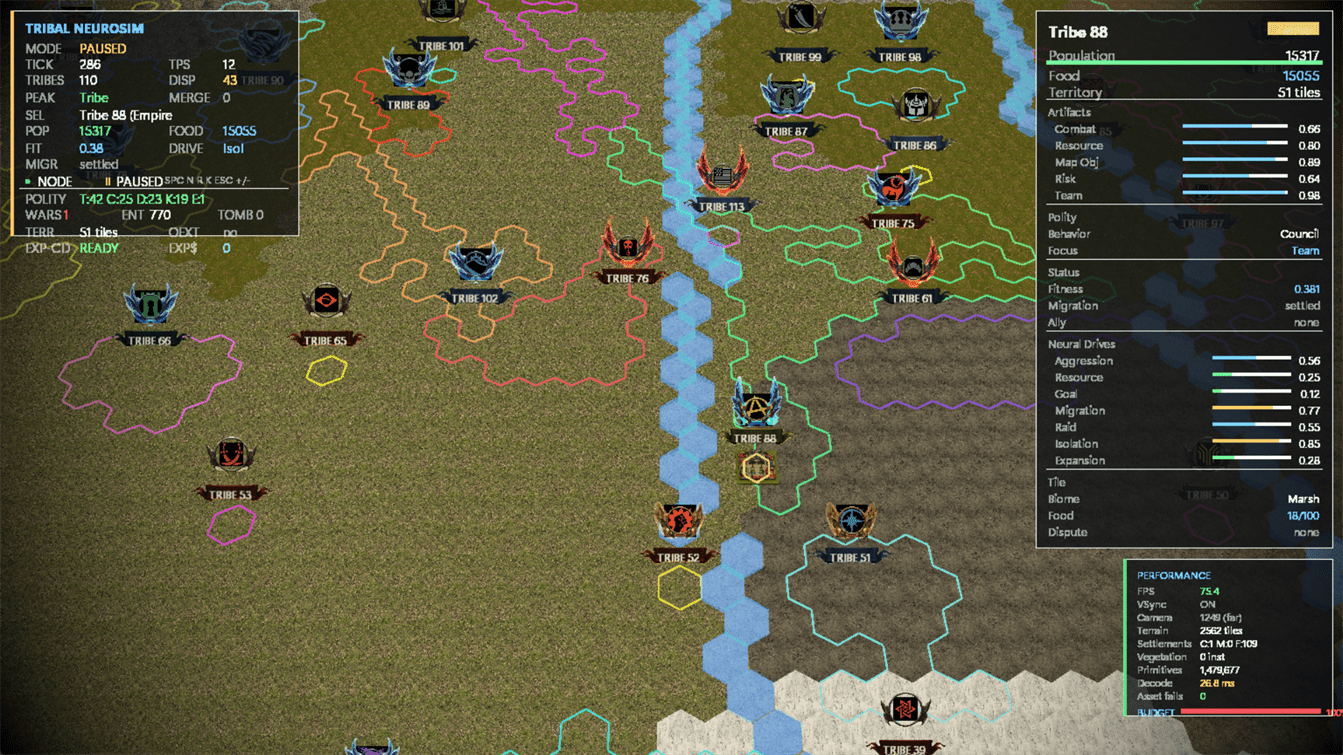
\includegraphics[width=0.9\textwidth]{assets/neurosim/run67sq42-sq-s42-tick286-firstempire.png}
\caption{SoloQ, seed=42, tick=286: az első Empire, Tribe 88, Council / Team profillal.}
\label{fig:neurosim-run-sq42-firstempire}
\end{figure}

\begin{figure}[h]
\centering
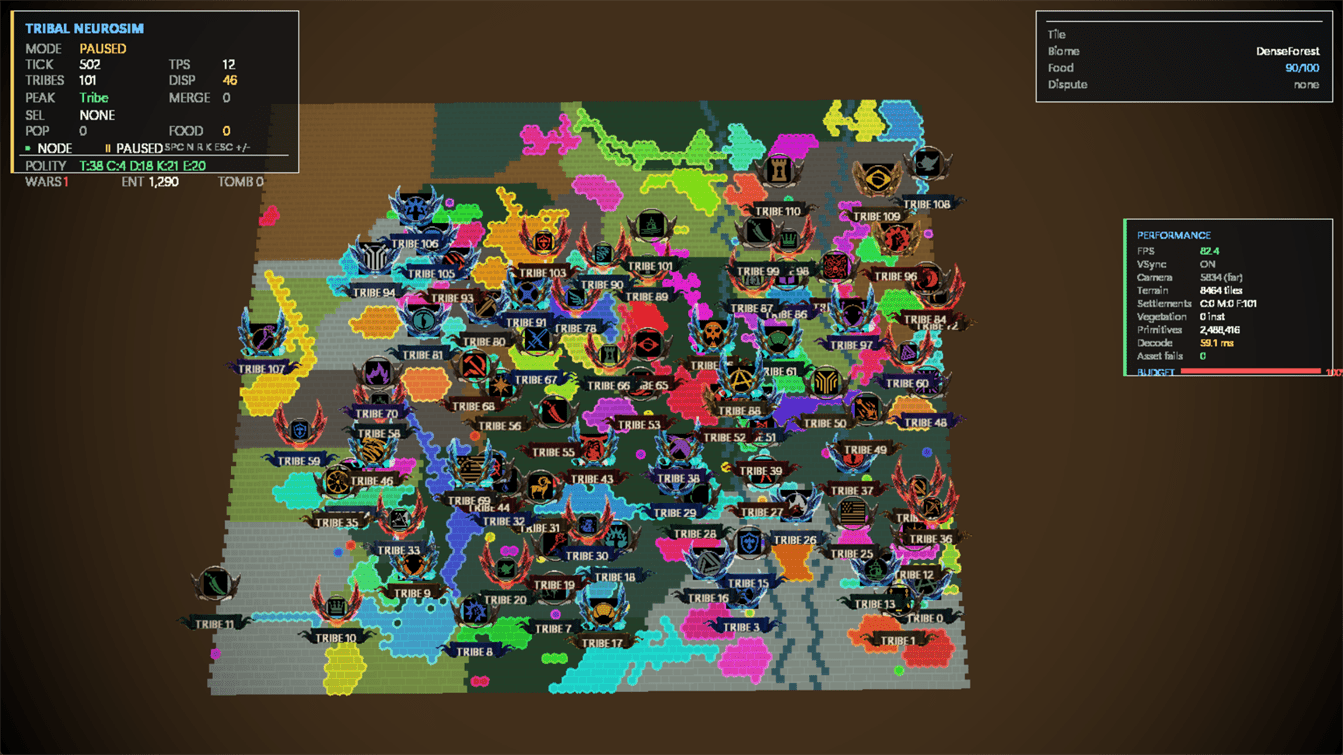
\includegraphics[width=0.9\textwidth]{assets/neurosim/run67sq42-sq-s42-tick500.png}
\caption{SoloQ, seed=42, tick=500: 101 túlélő a kis, sűrű térképen.}
\label{fig:neurosim-run-sq42-tick500}
\end{figure}

\begin{figure}[h]
\centering
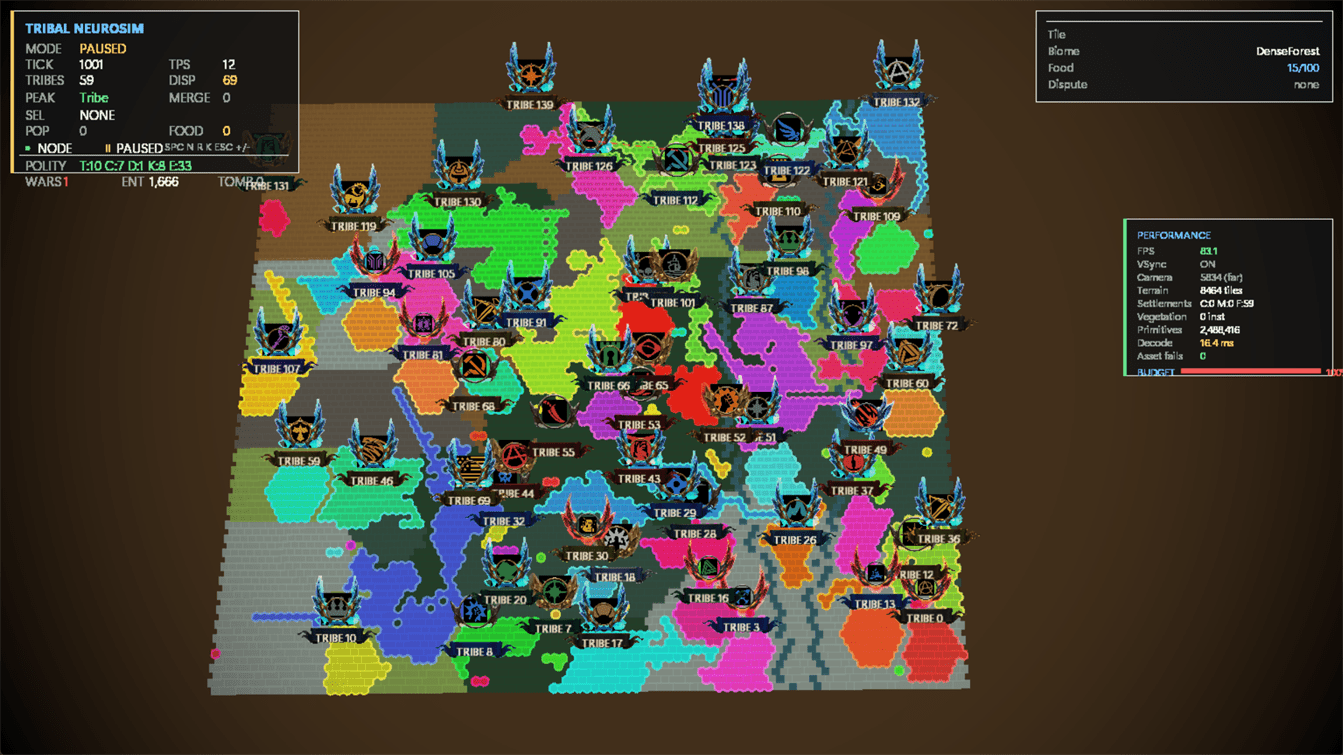
\includegraphics[width=0.9\textwidth]{assets/neurosim/run67sq42-sq-s42-tick1000.png}
\caption{SoloQ, seed=42, tick=1000: 59 túlélő, 33 Empire; a térkép nagy része már lefedett.}
\label{fig:neurosim-run-sq42-tick1000}
\end{figure}

\begin{figure}[h]
\centering
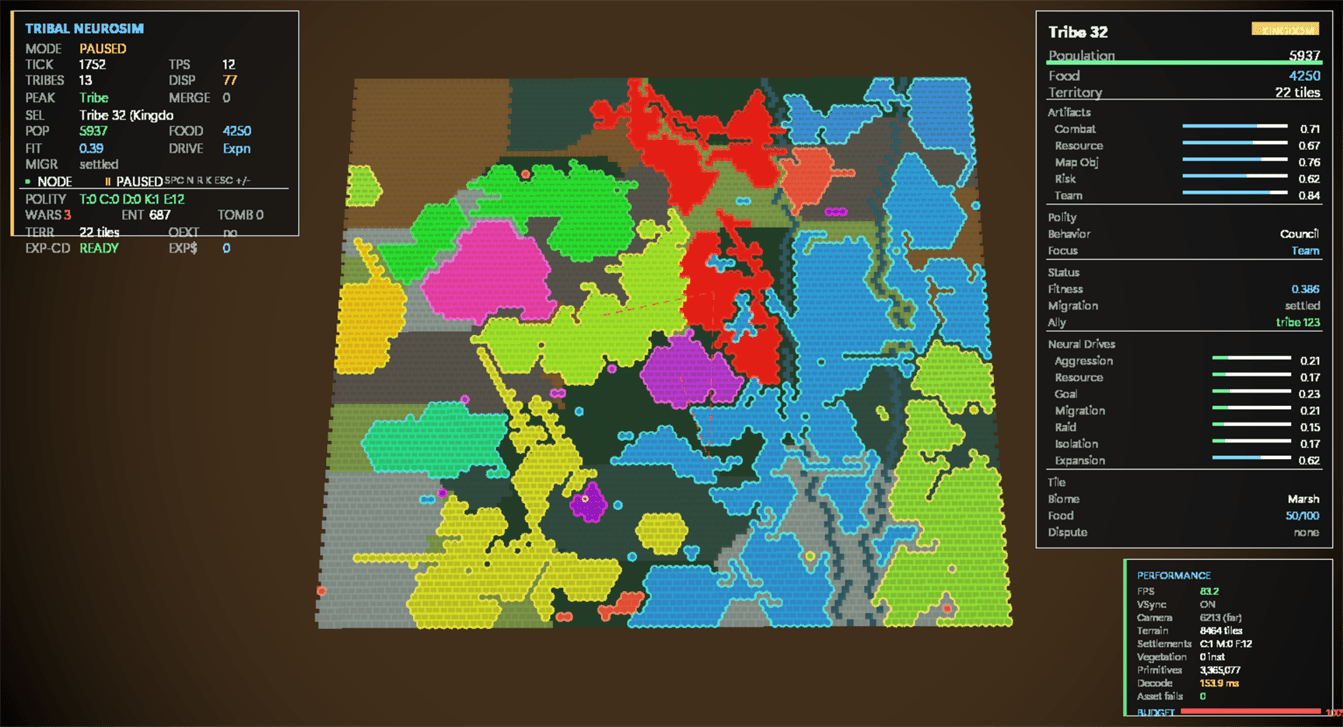
\includegraphics[width=0.9\textwidth]{assets/neurosim/run67sq42-sq-s42-tick1752-totalwar.png}
\caption{SoloQ, seed=42, tick=1752: a tick=1740-es Total War utáni állapot, 13 túlélővel és 5 aktív háborúval.}
\label{fig:neurosim-run-sq42-totalwar}
\end{figure}

\begin{figure}[h]
\centering
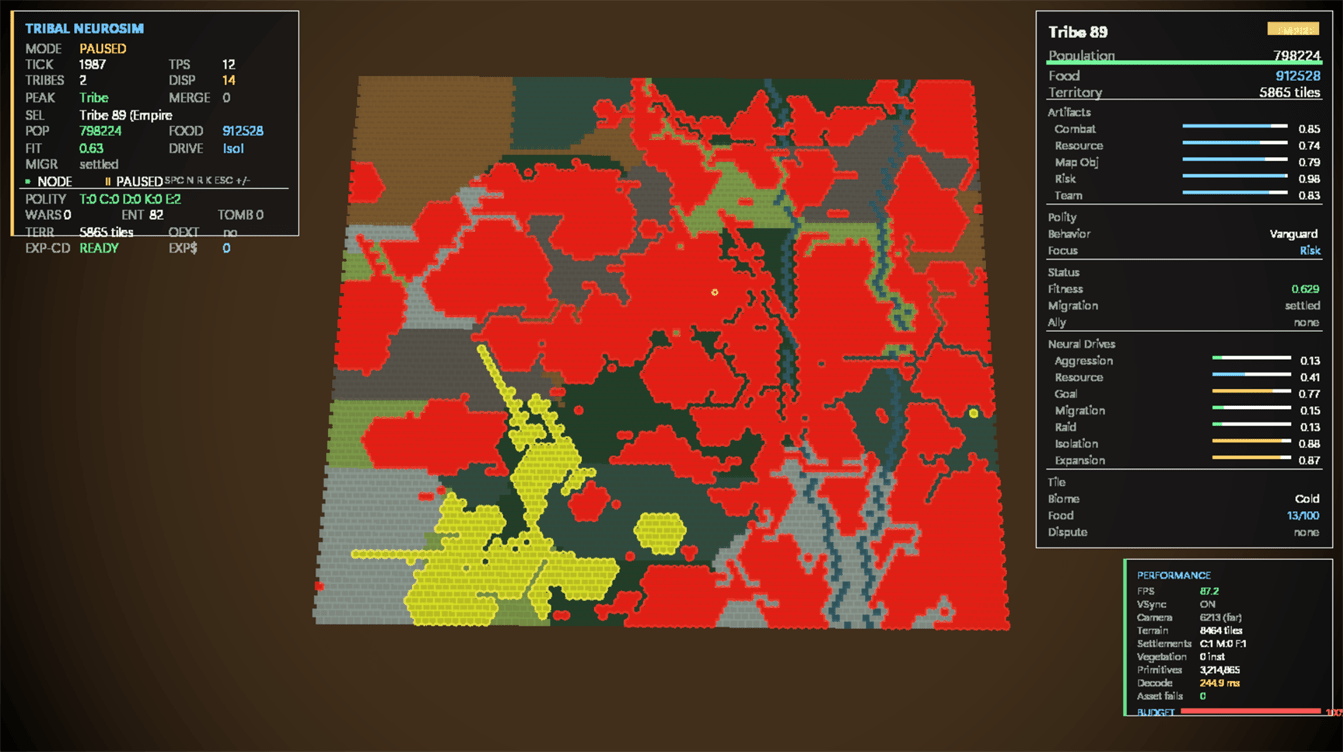
\includegraphics[width=0.9\textwidth]{assets/neurosim/run67sq42-sq-s42-tick1987-last2A.png}
\caption{SoloQ, seed=42, tick=1987: végső két szereplő, Tribe 89 domináns területi helyzetben.}
\label{fig:neurosim-run-sq42-last2a}
\end{figure}

\begin{figure}[h]
\centering
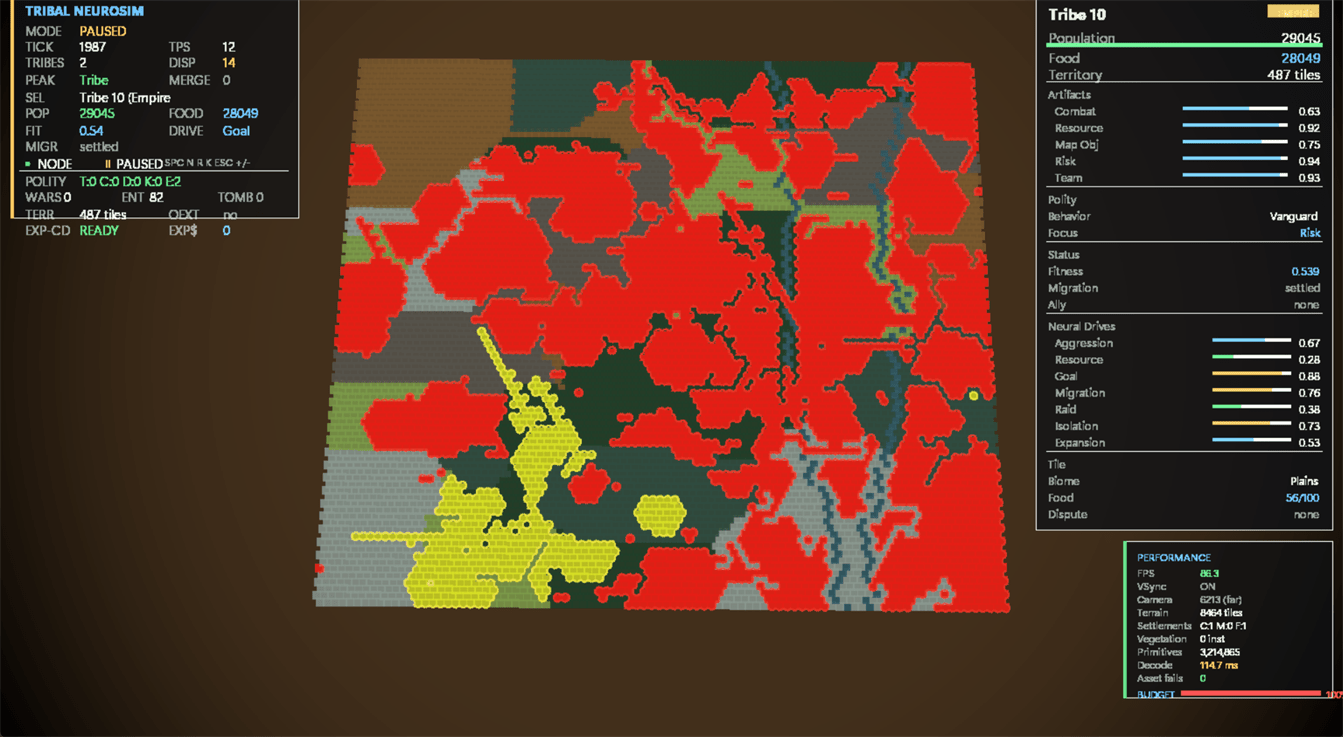
\includegraphics[width=0.9\textwidth]{assets/neurosim/run67sq42-sq-s42-tick1987-last2B.png}
\caption{SoloQ, seed=42, tick=1987: végső két szereplő, Tribe 10 sarokba szorított állapotban.}
\label{fig:neurosim-run-sq42-last2b}
\end{figure}

\begin{figure}[h]
\centering
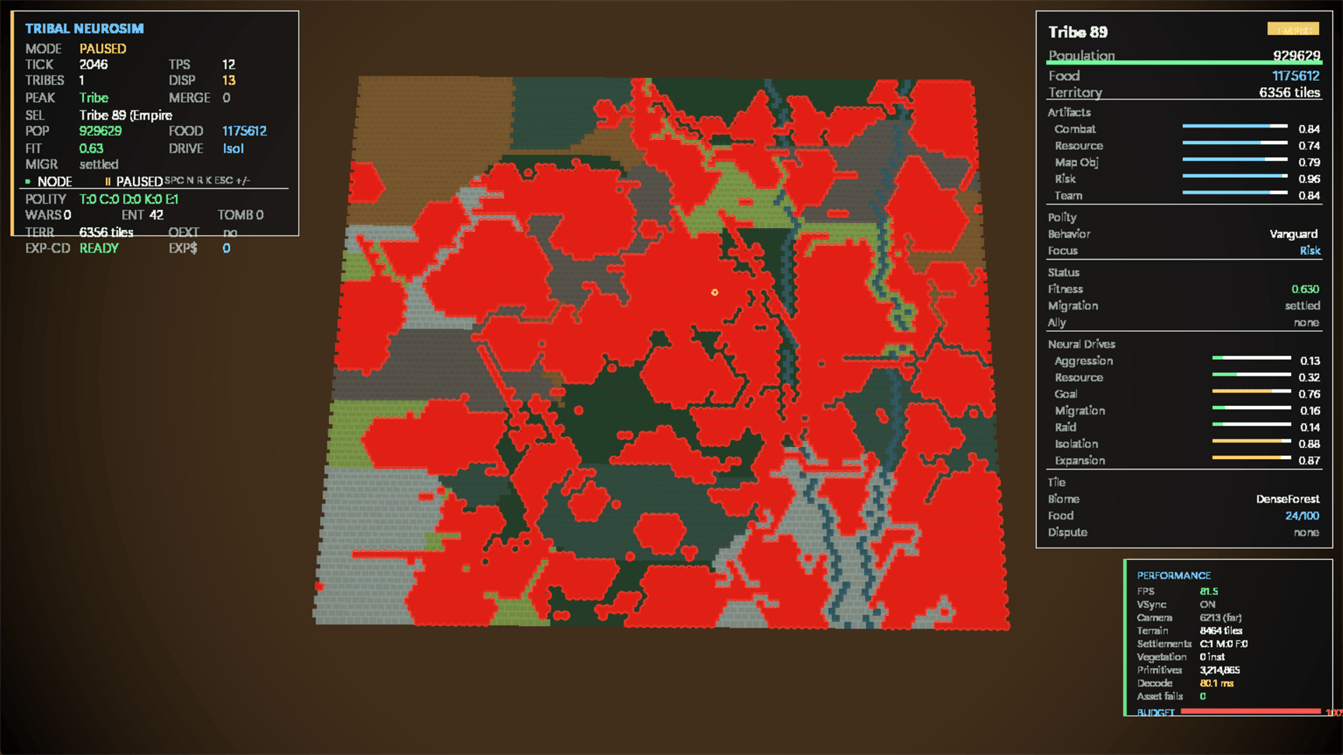
\includegraphics[width=0.9\textwidth]{assets/neurosim/run67sq42-sq-s42-tick2046-last.png}
\caption{SoloQ, seed=42, tick=2046: Tribe 89 győzelme, 6\,356 tile-os végső területtel.}
\label{fig:neurosim-run-sq42-last}
\end{figure}

\subsection*{SoloQ, seed=7777}

\begin{table}[h]
\centering
\caption{SoloQ seed=7777 futtatás összefoglalója}
\label{tab:neurosim-run-sq7777-summary}
\begin{tabular}{ll}
\hline
\textbf{Mező} & \textbf{Érték} \\
\hline
Adatkészlet & soloq (EUNE Master+ Solo Queue) \\
Seed & 7777 \\
Indítótörzsek & 140 \\
Térkép & végső győztes terület: 9\,748 tile \\
Végső tick & 2541 \\
Győztes & Tribe 70 \\
Behavior / fókusz & Empire / Supply / Resource \\
Agresszió & 0,88 \\
Migráció / izoláció / raid & 0,87 / 0,88 / 0,43 \\
Kulcsesemény & Tribe 99 középső dominanciája, majd tick=2340-es bukása \\
\hline
\end{tabular}
\end{table}

A SoloQ seed=7777 futtatás 140 törzzsel és tick=2541-es végállapottal zárult. A győztes Tribe 70 Empire / Supply / Resource profilú entitás volt, 0,88-as agresszióval, 0,87-es migrációval, 0,88-as isolation értékkel és 0,43-as raid drive-val a győztes képernyőkép alapján. Ez a negyedik futtatás teszi explicitté az adatkészlet-függő archetípus-különbséget: ugyanazzal a seed-del a flexset Warband / Combat győztest adott, míg a SoloQ Supply / Resource győztest, magas agressziós és resource komponenssel.

A korai szakasz nyugodtabb volt, mint a flexset megfelelője. Tick=50-nél mind a 140 törzs élt, tick=100-nál csak egy törzs esett ki. Az első Empire tick=300-nál jelent meg, a tick=301-es képen Tribe 19 látható Warband / Combat profillal, 10\,844 populációval, 47 tile-lal és 0,33-as fitnesszel. Ekkor 122 törzs volt életben, tehát az Empire-küszöb korai elérése itt sem jelentett végső dominanciát; Tribe 19 csak tick=2505-nél esett ki, vagyis polity-szint szerint a futtatás egyik leghosszabb túlélője maradt.

A középső szakasz főszereplője Tribe 99 volt. A log szerint már tick=147-nél legyőzte Tribe 100-at, majd hosszú sorozatban további győzelmeket aratott: Tribe 76 tick=387-nél, Tribe 61 tick=1239-nél, Tribe 101 tick=1392-nél, Tribe 92 tick=1692-nél, Tribe 85 tick=1935-nél és Tribe 124 tick=2091-nél esett ki ellene. A napló ezen kívül több védelmi győzelmet is rögzít Tribe 99 körül, ezért itt nem egyetlen csatáról, hanem tartós front-runner szerepről van szó. Ez a minta a SoloQ futtatások individualizáltabb, front-runner jellegű dinamikáját mutatja.

Tick=1000 és tick=2000 között a futtatás hosszú stagnációt produkált. Tick=1000-nél 61, tick=1500-nál 40, tick=1850-nél még mindig 32 törzs élt; tick=1550 és tick=1850 között az alive count alig mozdult. A térkép ekkorra nagyrészt felosztottá vált, a nagy Empire-ek pedig ritkábban találtak kedvező opportunista támadási ablakot. A flexset tömeges kaszkádjaihoz képest ez lassabb, egyéni háborúkra épülő konszolidáció.

A Totális Háború tick=2100-nál indult, 17 egyidejű opportunity war deklarációval. Tick=2110-nél 18 túlélő, 7 aktív háború és kizárólag Empire-szintű szereplők láthatók. A kaszkád tick=2150-re 13, tick=2200-ra 11, tick=2250-re 8, tick=2300-ra 6 túlélőt hagyott. A 23.4.~alszekció konfliktustípusai szerint ez kisebb abszolút méretű, de a megmaradt mezőnyhöz képest erős opportunista konfliktusburst.

A végjáték legfontosabb fordulata tick=2340-nél történt: Tribe 99, a középső szakasz domináns támadója, kiesett. A napló szerint Tribe 45 támadóként győzte le, miközben Tribe 97 is része volt a többfrontos nyomásnak. Tick=2409-nél Tribe 70 legyőzte Tribe 97-et, tick=2460-nál Tribe 119 kétfrontos helyzetben esett ki, majd tick=2505-nél az első Empire, Tribe 19 támadta Tribe 70-et és védőként vereséget szenvedett. Tick=2510-nél már csak Tribe 45 és Tribe 70 maradt: Tribe 45 Vanguard / Risk profilként 4\,164 tile-t és 550\,659 populációt tartott, míg Tribe 70 Supply / Resource profilként 5\,583 tile-t és 849\,134 populációt. Tick=2520-nál Tribe 45 még opportunity raid-et indított, de tick=2541-nél Tribe 70 győzött, 244\,172 populációval, 943\,489 food tartalékkal és 9\,748 tile-lal.

\begin{figure}[h]
\centering
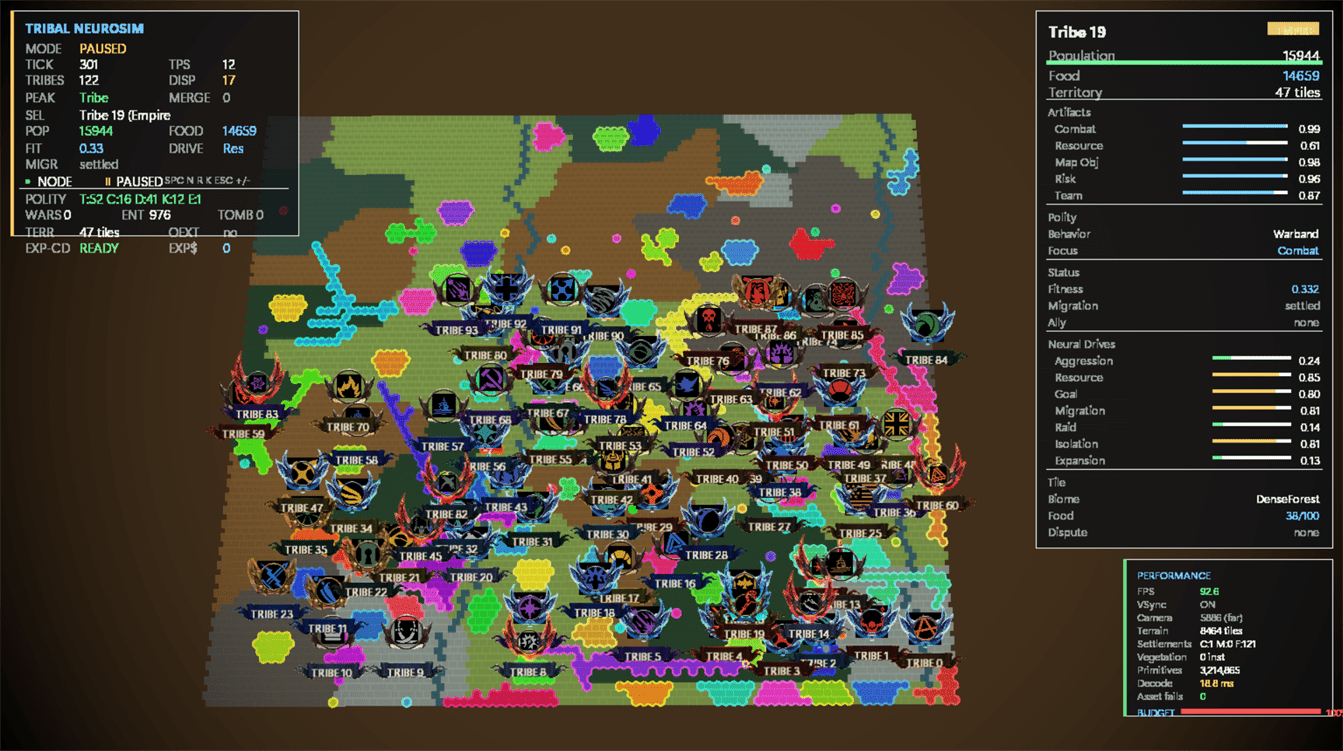
\includegraphics[width=0.9\textwidth]{assets/neurosim/run67sq7777-sq-s7777-tick301-firstempire.png}
\caption{SoloQ, seed=7777, tick=301: az első Empire, Tribe 19, Warband / Combat profillal.}
\label{fig:neurosim-run-sq7777-firstempire}
\end{figure}

\begin{figure}[h]
\centering
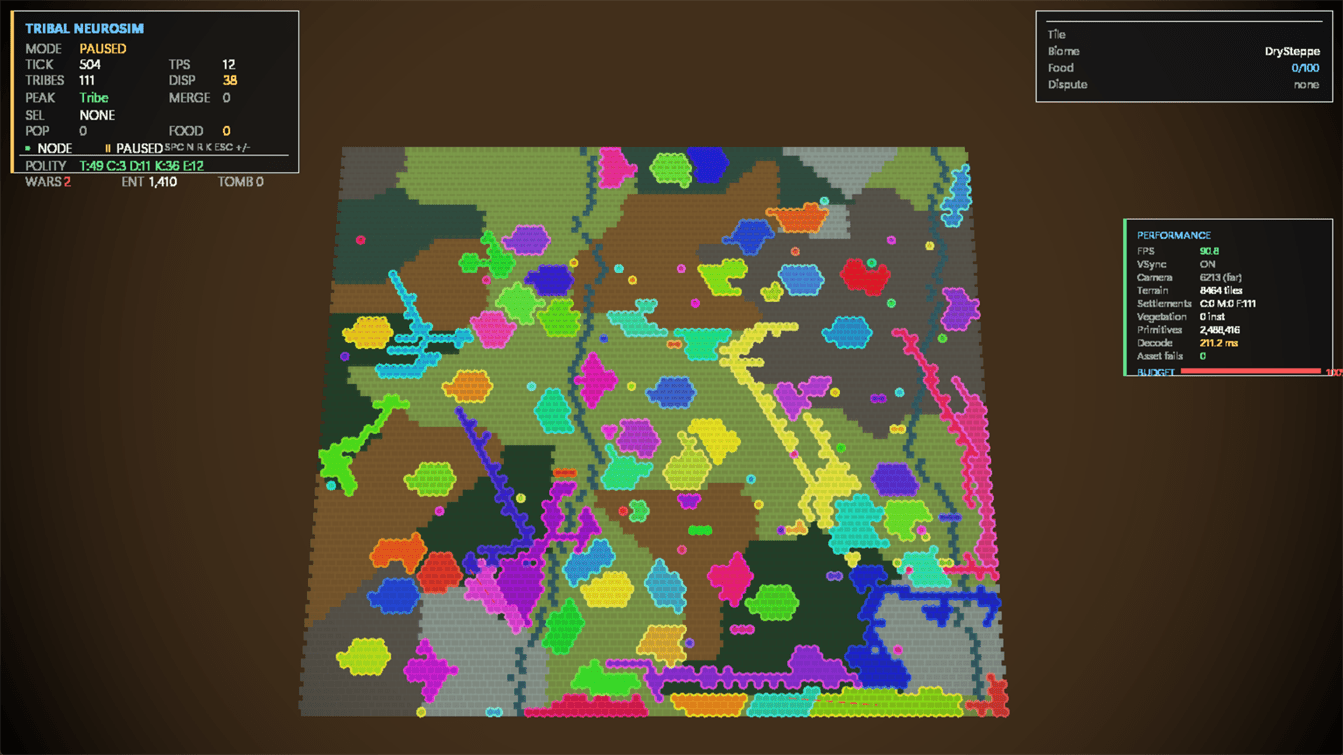
\includegraphics[width=0.9\textwidth]{assets/neurosim/run67sq7777-sq-s7777-tick500.png}
\caption{SoloQ, seed=7777, tick=500: 111 túlélő, még jelentős elválasztott területi foltokkal.}
\label{fig:neurosim-run-sq7777-tick500}
\end{figure}

\begin{figure}[h]
\centering
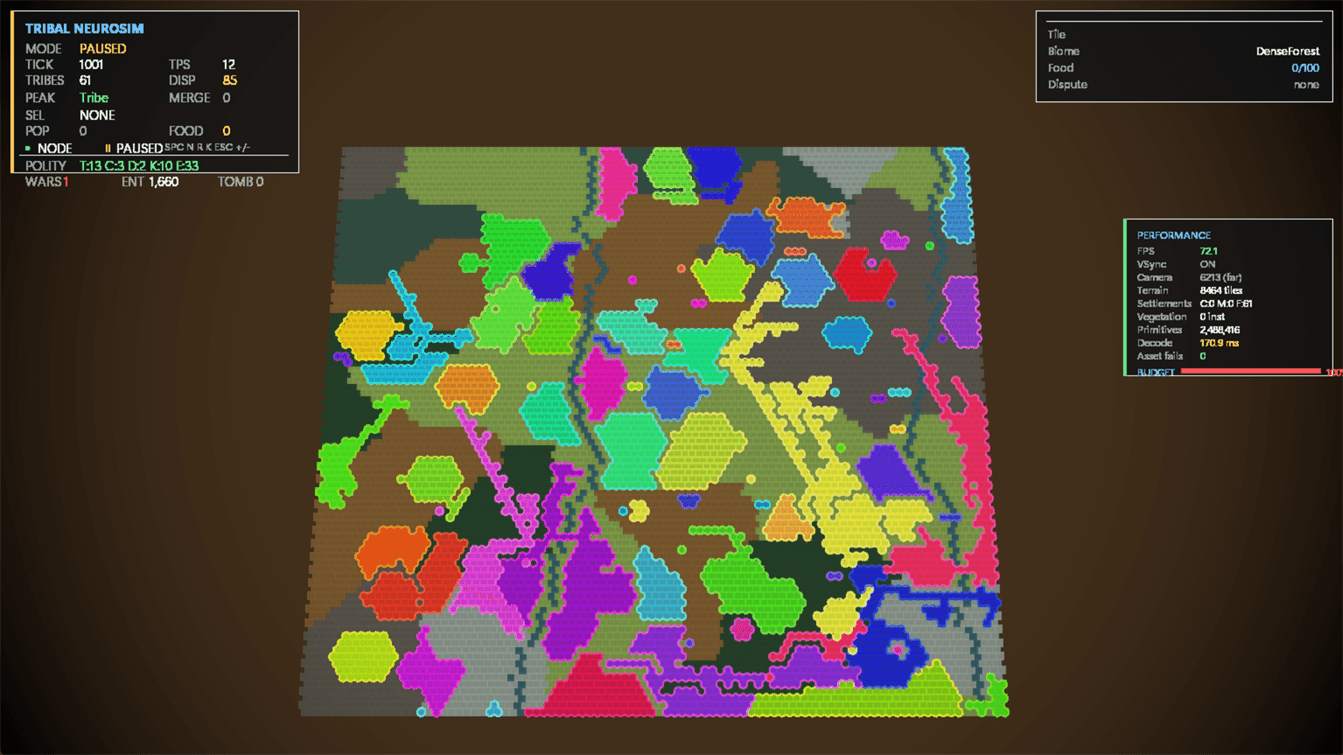
\includegraphics[width=0.9\textwidth]{assets/neurosim/run67sq7777-sq-s7777-tick1000.png}
\caption{SoloQ, seed=7777, tick=1000: 61 túlélő, 33 Empire; a középső stagnáció előtti állapot.}
\label{fig:neurosim-run-sq7777-tick1000}
\end{figure}

\begin{figure}[h]
\centering
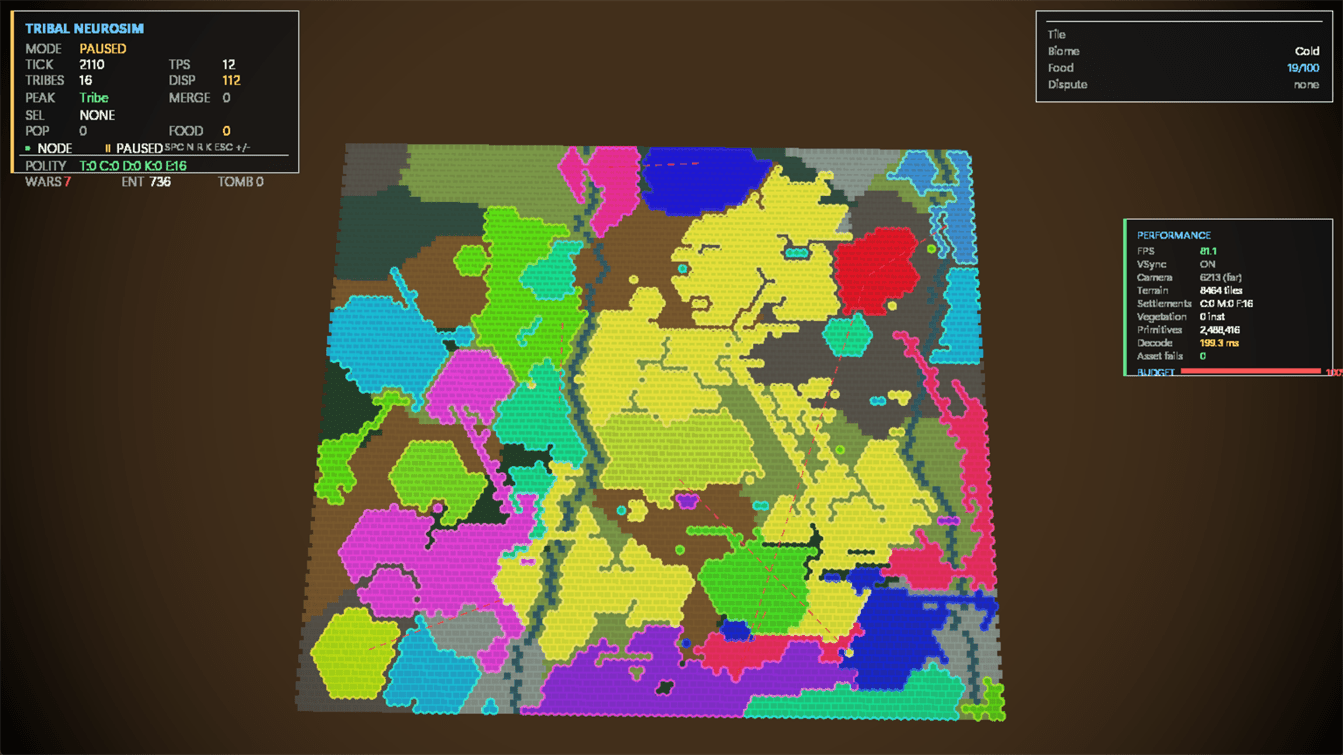
\includegraphics[width=0.9\textwidth]{assets/neurosim/run67sq7777-sq-s7777-tick2100-totalwar.png}
\caption{SoloQ, seed=7777, tick=2110: a tick=2100-as Total War utáni állapot, 18 túlélővel és 7 aktív háborúval.}
\label{fig:neurosim-run-sq7777-totalwar}
\end{figure}

\begin{figure}[h]
\centering
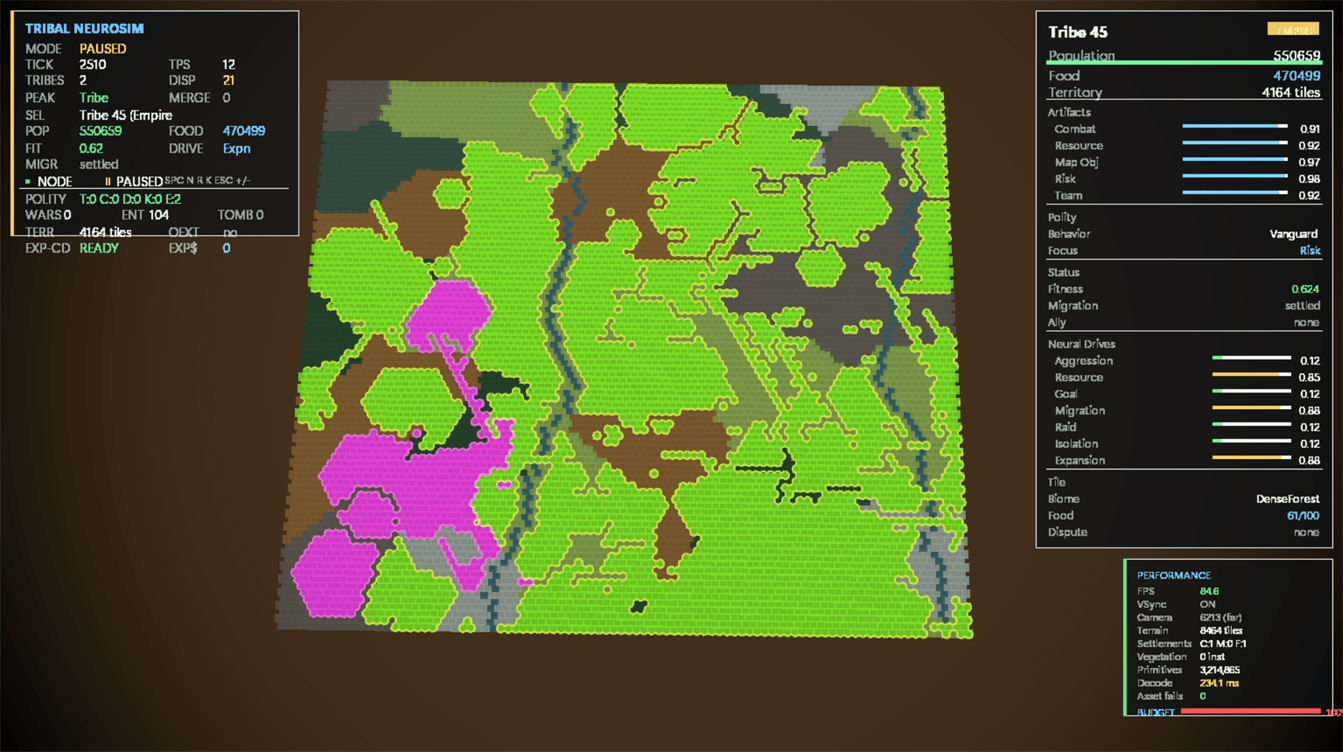
\includegraphics[width=0.9\textwidth]{assets/neurosim/run67sq7777-sq-s7777-tick2510-last2A.png}
\caption{SoloQ, seed=7777, tick=2510: végső két szereplő, Tribe 45 Vanguard / Expansion profillal.}
\label{fig:neurosim-run-sq7777-last2a}
\end{figure}

\begin{figure}[h]
\centering
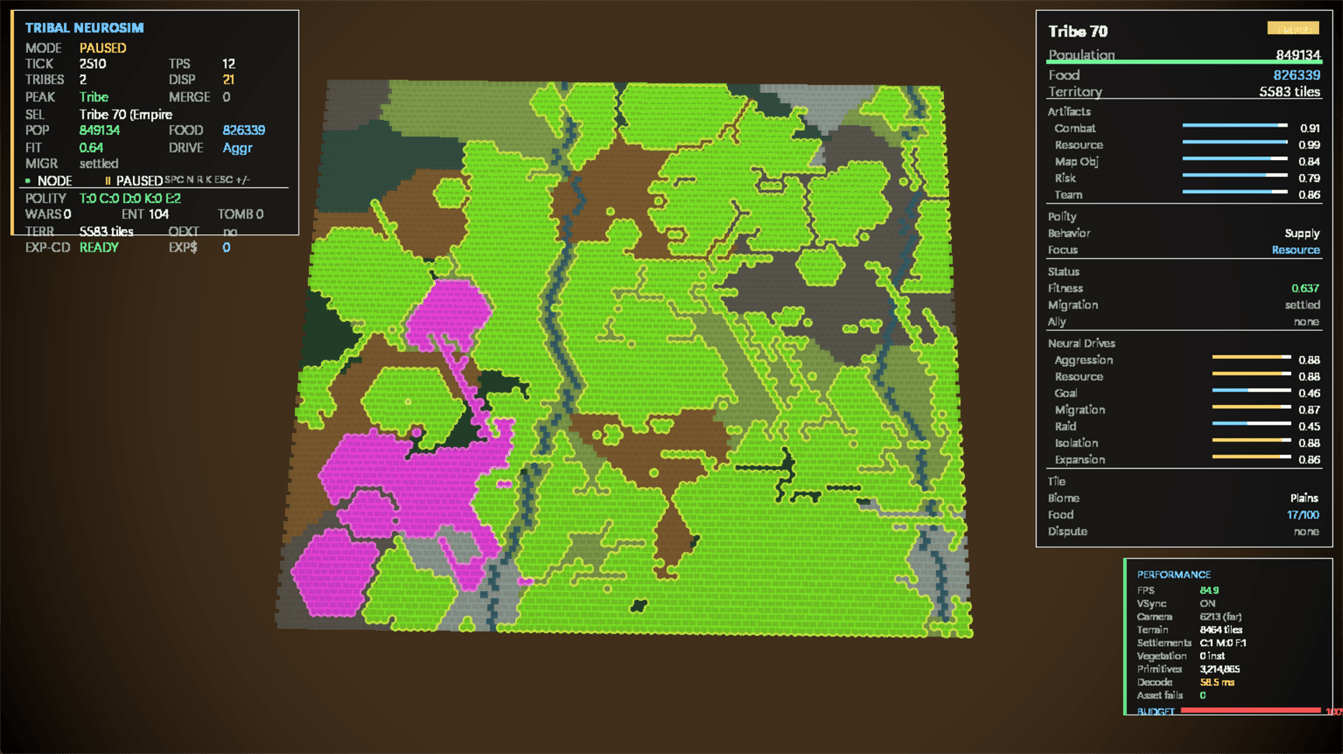
\includegraphics[width=0.9\textwidth]{assets/neurosim/run67sq7777-sq-s7777-tick2510-last2B.png}
\caption{SoloQ, seed=7777, tick=2510: végső két szereplő, Tribe 70 Supply / Resource profillal.}
\label{fig:neurosim-run-sq7777-last2b}
\end{figure}

\begin{figure}[h]
\centering
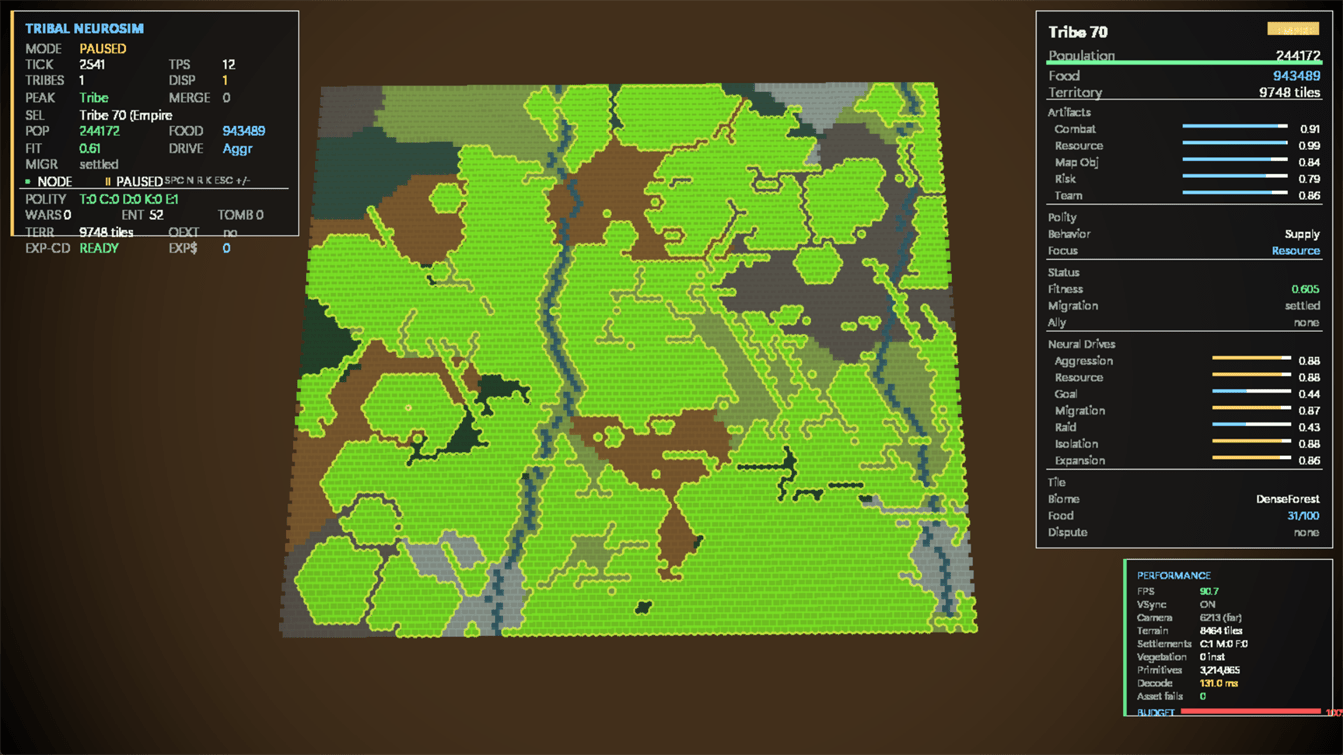
\includegraphics[width=0.9\textwidth]{assets/neurosim/run67sq7777-sq-s7777-tick2541-last.png}
\caption{SoloQ, seed=7777, tick=2541: Tribe 70 győzelme, 9\,748 tile-os végső területtel.}
\label{fig:neurosim-run-sq7777-last}
\end{figure}

% ==========================================================================
\section{Miért képesek kisebb törzsek nagyobbakat legyőzni}
\label{sec:neurosim-26-upset}
% ==========================================================================

A négy futtatás eseménynaplóiban többször megfigyelhető egy első ránézésre
meglepő jelenség: egy, a domináns entitásnál területileg, populációban
és erőforrásokban jelentősen kisebb törzs képes azt legyőzni és abszorbeálni.
A flexset seed=42 futtatásban Tribe~596 kevesebb területtel rendelkezett, mint
Tribe~557, mégis megnyerte a háborút tick=2424-nél. A SoloQ seed=7777 futtatásban
Tribe~45 legyőzte a tartósan domináns Tribe~99-et tick=2340-nél.

Ennek mechanikai magyarázata három tényező kombinációja.

\textbf{Felhalmozott $A\_\text{combat}$ előny.} Az $A\_\text{combat}$ artifaktum minden megnyert
védelmi háborúval növekszik, de csak a ténylegesen megnyert harci körök után.
Egy kis törzs, amelyik több védelmi háborút nyert, magasabb $A\_\text{combat}$-tal
rendelkezhet, mint egy nagy törzs, amelyik expanzióval, nem harccal növekedett.
A Poisson-veszteség képletéből következően ez a különbség non-lineárisan hat:
ha $a_{\text{kis}} > a_{\text{nagy}}$, a kis törzs várható vesztesége alacsonyabb
tick-enként, még ha kontaktzónája kisebb is.

\textbf{Kétfrontos nyomás.} Ahogy a 25.4.~alszakasz tárgyalja, a domináns entitás
egyszerre több szomszéddal kerülhet háborúba. Ha két kisebb törzs egymástól
függetlenül ugyanazon tickben indít háborút a nagyobb ellen --- mint a trilaterális
esetben ---, a Poisson-veszteség mindkét fronton akkumulálódik. A nagy törzs
populációja és élelmiszer-készlete egyszerre csökken, miközben csak az egyik
ellenfelet tudja visszaverni.

\textbf{Erőforrás-szűkösség.} A nagy törzs magas territory fenntartási költsége
és a háborús állapotban szünetelő élelmiszer-gyűjtés (starvation cascade jelenség,
ld. 26.2.~alszakasz) fokozatosan csökkenti a harci kapacitást. Egy kisebb, mobilis
ellenfél számára ez ablakot nyit: a nagy törzs katonailag még erős, de logisztikailag
sérülékeny.

Összefoglalva: a szimuláció nem biztosítja a méretarányos fölényt. A méret
előny az erőforrástermelésben és a területi jelenlétben, de hátrány a
kétfrontos nyomással szemben és a logisztikai kitettségben. Ez a dinamika
teszi a végső szakaszt nehezen előrejelezhetővé, és hozzájárul ahhoz, hogy
a futtatási narratívák genuinisan emergensnek hatnak.

% ==========================================================================
\section{Adatkészlet-összehasonlítás és értelmezési határok}
\label{sec:neurosim-26-conclusions}
% ==========================================================================

A négy validált Tribal NeuroSim futtatás közös értelmezése nem egyetlen győztes archetípus abszolút fölényéről szól, hanem arról, hogy eltérő adatkészletből származó klaszterpriorok azonos szimulációs szabályok alatt eltérő emergáló stratégiákat hoztak létre. A flexset és a soloq futtatások ugyanazt a szimulációs magot, azonos döntési logikát és determinisztikus seedelést használtak; a különbség a kezdeti klaszterprofilokban és az azok mögött álló gráfstruktúrában volt.

\subsection*{Összefoglaló táblázat}

\begin{table}[h]
\centering
\small
\caption{A négy záró Tribal NeuroSim futtatás összehasonlítása}
\label{tab:neurosim-run-comparison-final}
\resizebox{\textwidth}{!}{%
\begin{tabular}{llllllll}
\hline
\textbf{Futtatás} & \textbf{Adatkészlet} & \textbf{Seed} & \textbf{Győztes} & \textbf{Viselkedés} & \textbf{Agresszió} & \textbf{Migráció} & \textbf{Végső tick} \\
\hline
run67fl7777 & Flexset & 7777 & Tribe 355 & Warband/Combat & 0{,}18 & 0{,}88 & 2538 \\
run67fl42 & Flexset & 42 & Tribe 596 & Warband/Combat & 0{,}13 & 0{,}87 & 2487 \\
run67sq42 & SoloQ & 42 & Tribe 89 & Vanguard/Risk & 0{,}11 & 0{,}16 & 2046 \\
run67sq7777 & SoloQ & 7777 & Tribe 70 & Supply/Resource & 0{,}68 & 0{,}87 & 2541 \\
\hline
\end{tabular}
}
\end{table}

\begin{figure}[h]
\centering
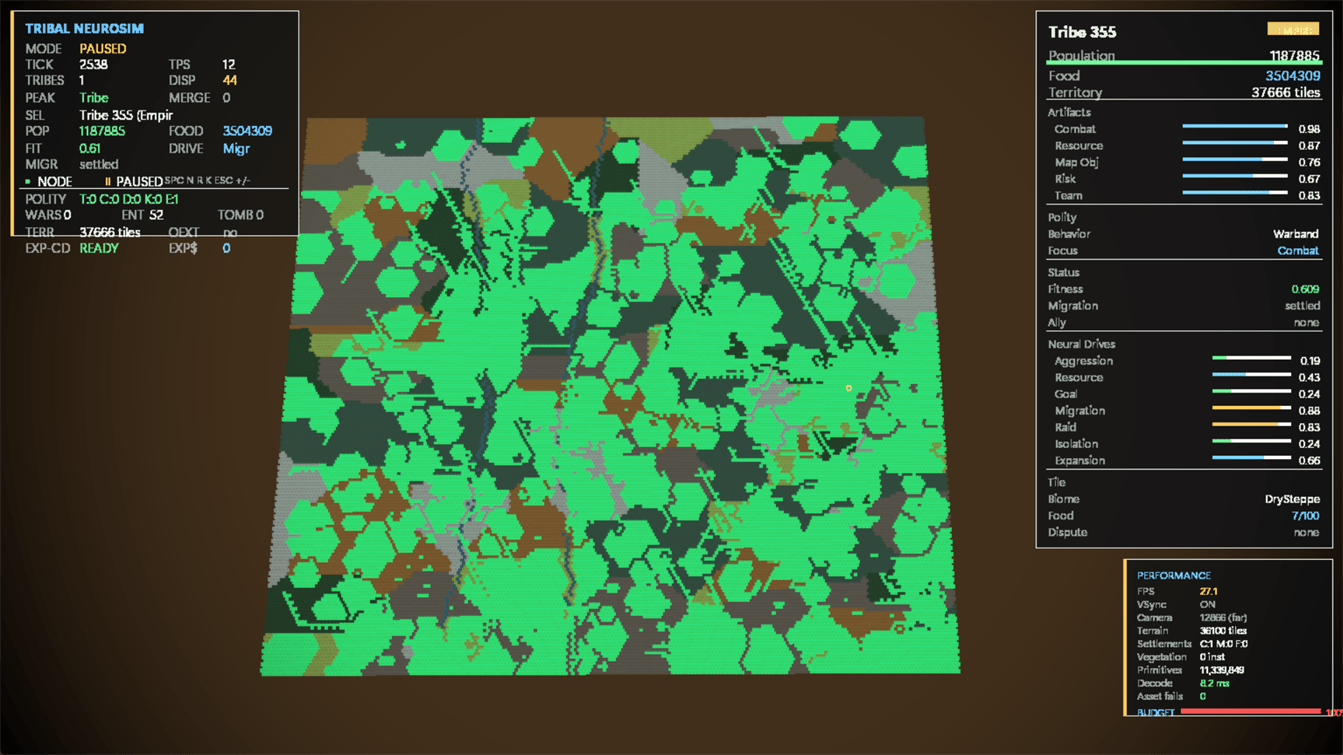
\includegraphics[width=0.9\textwidth]{assets/neurosim/run67fl7777-fl-s7777-tick2538-last.png}
\caption{Flexset, seed=7777, tick=2538: Tribe 355, Warband/Combat, 37\,666 tile}
\label{fig:neurosim-final-fl7777}
\end{figure}

\begin{figure}[h]
\centering
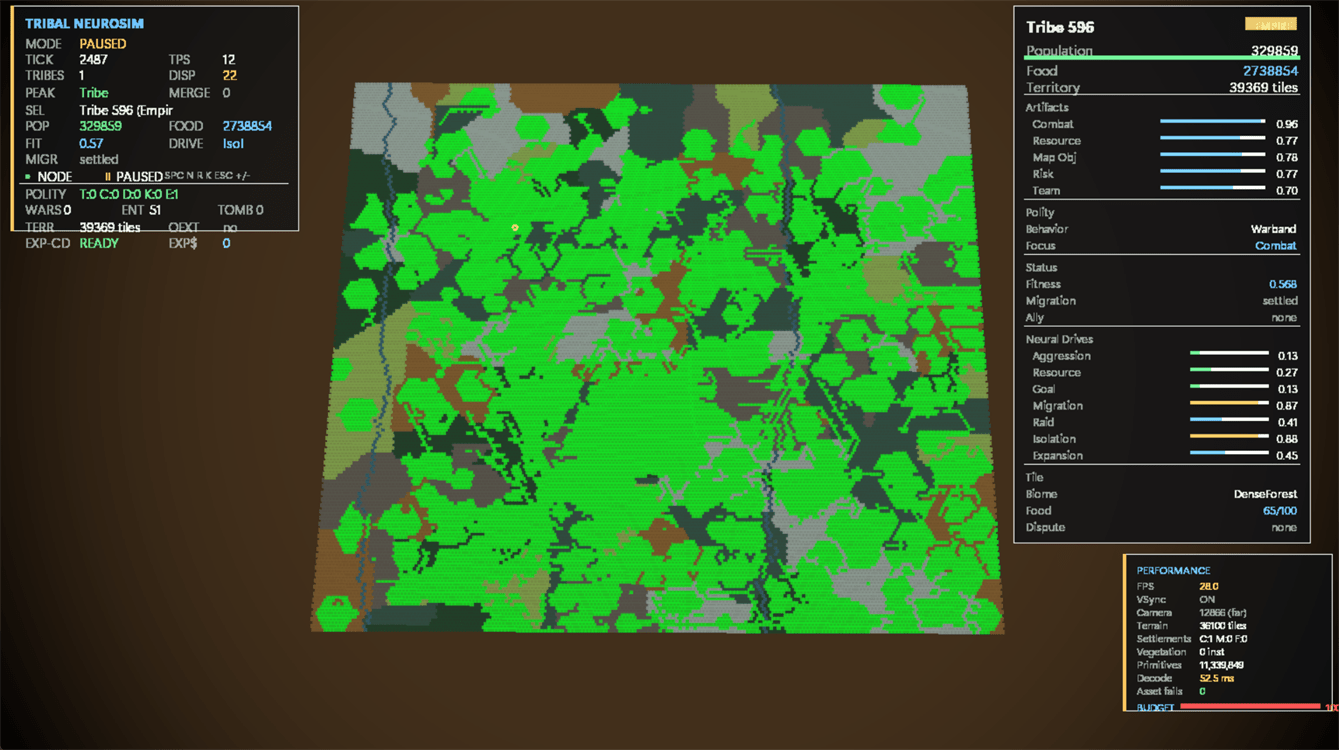
\includegraphics[width=0.9\textwidth]{assets/neurosim/run67fl42-fl-s42-tick2487-last.png}
\caption{Flexset, seed=42, tick=2487: Tribe 596, Warband/Combat, 39\,369 tile}
\label{fig:neurosim-final-fl42}
\end{figure}

\begin{figure}[h]
\centering
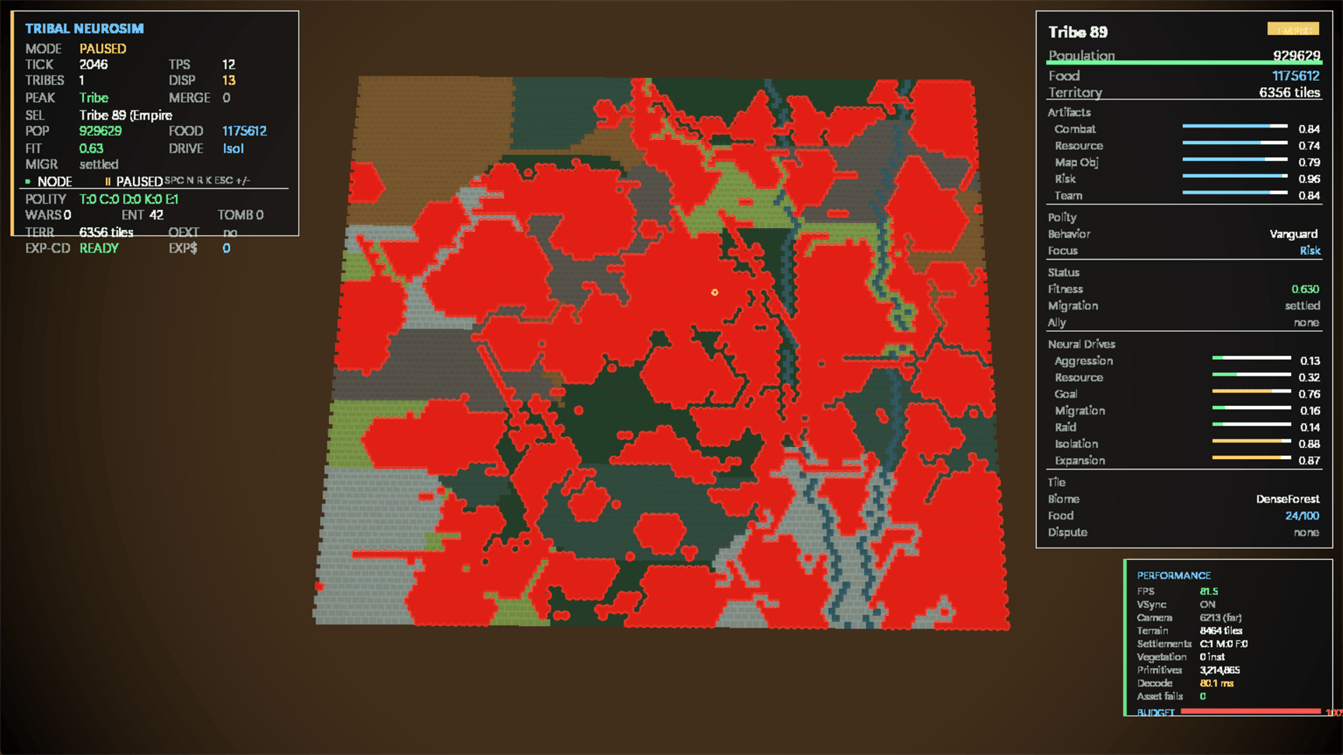
\includegraphics[width=0.9\textwidth]{assets/neurosim/run67sq42-sq-s42-tick2046-last.png}
\caption{SoloQ, seed=42, tick=2046: Tribe 89, Vanguard/Risk, 6\,356 tile}
\label{fig:neurosim-final-sq42}
\end{figure}

\begin{figure}[h]
\centering
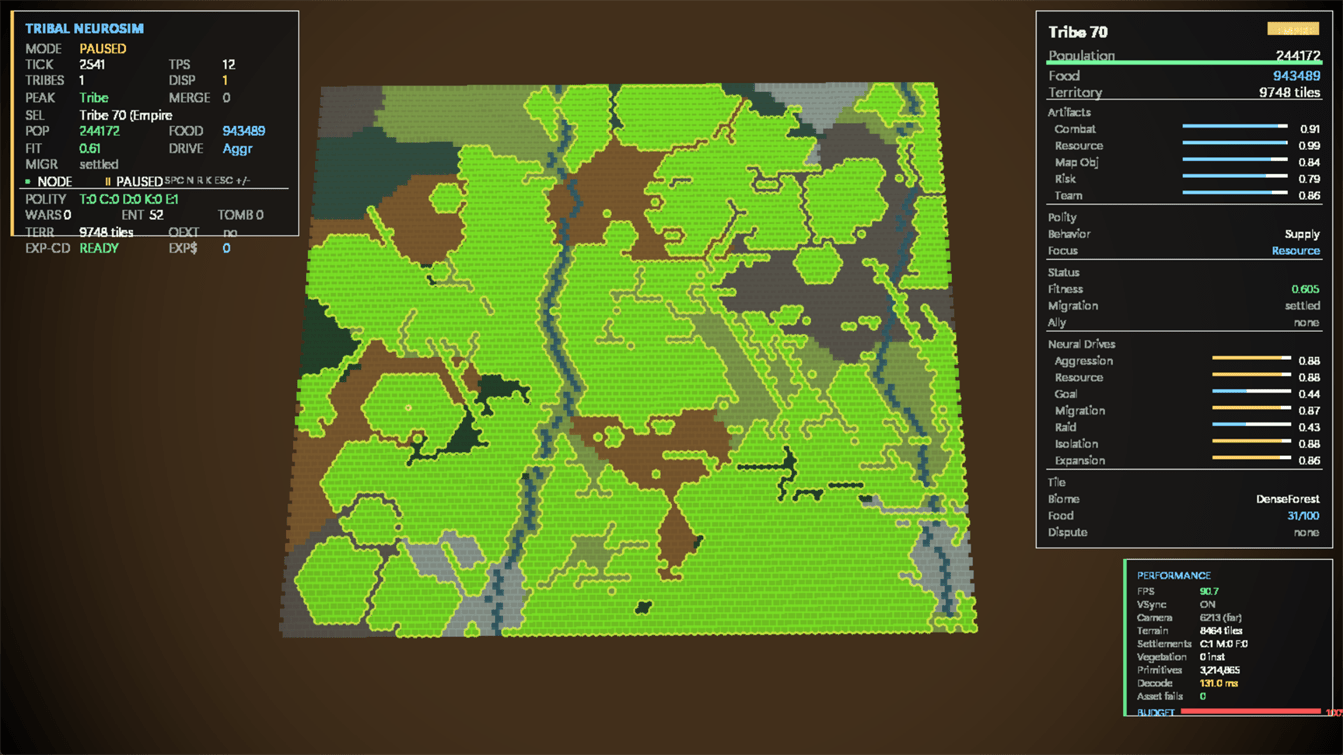
\includegraphics[width=0.9\textwidth]{assets/neurosim/run67sq7777-sq-s7777-tick2541-last.png}
\caption{SoloQ, seed=7777, tick=2541: Tribe 70, Supply/Resource, 9\,748 tile}
\label{fig:neurosim-final-sq7777}
\end{figure}

\subsection*{Kulcsmegállapítás: konvergencia és variabilitás}

A legfontosabb eredmény a flexset és a soloq futtatások közötti konvergencia--variabilitás különbség. A két flexset futtatás eltérő seed mellett ugyanarra a győztes viselkedési archetípusra futott ki: mindkét esetben Warband/Combat profilú entitás maradt életben. A győztesek agressziója alacsony volt, 0{,}13--0{,}18 közötti tartományban, miközben a migrációs hajtóerő nagyon magas maradt, 0{,}87--0{,}88 körül. A kapcsolódó izolációs értékek szintén magasak, megközelítőleg 0{,}88 körüliek voltak. Ez olyan stratégiai mintát ír le, amely nem folyamatos támadással, hanem területfoglalással, önálló pozíciótartással és felhalmozott harci kompetenciával nyert.

A SoloQ futtatások ezzel szemben nem konvergáltak egyetlen archetípusra. Seed=42 mellett Tribe 89 Vanguard/Risk profillal nyert, alacsony agressziós és alacsony migrációs végállapottal; seed=7777 mellett Tribe 70 Supply/Resource profillal, magasabb agresszióval és magas migrációval zárta a futtatást. A két SoloQ győztes neurális profilja eltért egymástól, és az A\_combat felhalmozódási mintájuk sem ugyanazt a pályát követte: a seed=42 futtatásban a döntő szerep a védelmi túléléshez és célzott kockázatvállaláshoz kötődött, míg a seed=7777 futtatásban a resource-központú túlélés és az endgame-ben megnyíló opportunista ablak volt meghatározó.

Ez a divergencia a mögöttes gráfstruktúra különbségéből értelmezhető. A flexset adatkészlet szervezettebb, ismétlődő kapcsolatmintákat hordoz, míg a soloq adatkészlet inkább egyéni teljesítményprofilokat rögzít tartós co-queue struktúra nélkül. A szimulációs különbség ezért nem pusztán seed-zajként, hanem a klaszterpriorok eltérő szerkezetének következményeként olvasható.

\subsection*{Értelmezési keret}

A Flex Queue klaszterek koordinált csapatjátékot kódolnak. A flexset gráfban az alliance jellegű minták, a komplementer szerepek és az ismétlődő co-queue kapcsolatok nem egyetlen játékos izolált teljesítményét, hanem visszatérő együttjátszási struktúrákat írnak le. Amikor ezekből klaszterprofilok készülnek, a szimuláció olyan entitásokat inicializál, amelyekben a harci kompetencia, a területi önfenntartás és a magas izoláció egyszerre jelenhet meg. A két flexset futtatás Warband/Combat konvergenciája ebben az értelmezésben nem azt jelenti, hogy ez a profil objektíven jobb minden környezetben, hanem azt, hogy ebben a klaszterezési és szabálykörnyezetben stabilan újra megjelent.

A SoloQ klaszterek más jellegű információt hordoznak. Ezek nem tartós társas csapatstruktúrát, hanem rangsorolt egyéni teljesítményprofilokat sűrítenek. A SoloQ inicializáció ezért kevésbé ad át olyan koordinált társas mintát, amely több seed alatt is ugyanabba a túlélési stratégiába húzná a rendszert. Ennek megfelelően a seed=42 futtatás Vanguard/Risk, a seed=7777 futtatás Supply/Resource győztest produkált, vagyis a szimulált kimenet változékonyabb lett.

Az értelmezés korrelatív, nem okozati. Ahogy a 24.3.~alszakasz validációs megfogalmazása is hangsúlyozza, a determinisztikus és esemény-alapon visszaellenőrizhető futtatás azt igazolja, hogy adott klaszterpriorok mellett milyen szimulált dinamika jött létre. Nem igazolja, hogy a valódi játékosok pszichológiai értelemben így viselkednének, és nem állít elő közvetlen LoL-meccs-előrejelzést.

\subsection*{Kiegészítő megfigyelések}

A SoloQ futtatásokban megjelent egy olyan minta, amely a flexset futtatásokból hiányzott: a domináns középső aktor. A SoloQ seed=7777 futtatásban Tribe 99 hosszú középső szakaszon át front-runnerként viselkedett, hét háborút nyert, majd tick=2340-nél mégis kiesett. Ez tiszta narratív ívet adott a futtatásnak: domináns szereplő, többfrontos nyomás, bukás, majd egy másik entitás győzelme. A flexset futtatásokban ezzel szemben a konszolidáció elosztottabb volt, több nagy szereplő párhuzamos nyomásával és kevésbé egyetlen központi midgame-hatalom köré szerveződve.

A futási sebesség értelmezésénél a térképméretet külön kell kezelni. A SoloQ seed=42 futtatás volt a leggyorsabb, tick=2046-os végállapottal, de ez nem önmagában SoloQ-tulajdonság. A futtatás kisebb, körülbelül 7000 tile-os térképen zajlott, ezért a kontaktus, a területi telítődés és a végső konszolidáció hamarabb következhetett be. A gyorsaság tehát részben térszubsztrátum-hatás, nem közvetlen adatkészlet-minősítés.

A Total War skála arányosabb képet ad, ha az indítótörzsek számához viszonyítjuk. A flexset futtatások 599 törzzsel indultak, és a nagy opportunista háborús burstök 55--72 deklarációs nagyságrendben jelentek meg. A SoloQ futtatások 140 törzzsel indultak, és a Total War események 15--17 deklarációs tartományban maradtak. Ez abszolút értékben kisebb, de a mezőny méretéhez viszonyítva továbbra is jelentős konfliktuskoncentrációt jelent.

\subsection*{Amit az eredmény alátámaszt, és amit nem}

Az eredmények alátámasztják, hogy a klaszter-derivált priorok mérhetően eltérő szimulált viselkedést produkálnak azonos szabálykörnyezetben. A flexset, mint koordináltabb gráfstruktúra, a két tesztelt seed alatt konvergens Warband/Combat kimenetelhez vezetett. A soloq, mint inkább egyéni teljesítményprofilokat hordozó adatkészlet, változékonyabb győztes archetípusokat produkált. A négy futtatás reprodukálható, inspektálható és esemény-alapon igazolt: a következtetések nem kizárólag a végső képernyőképekből, hanem a háborús, terjeszkedési és eliminációs események naplózott sorozatából származnak.

Az eredmények ugyanakkor nem bizonyítanak valódi játékos-pszichológiát. Nem állítják, hogy a Flex Queue játékosok szükségszerűen Warband-szerűen, a SoloQ játékosok pedig Vanguard- vagy Supply-szerűen viselkednek. Nem adnak előrejelzést tényleges League of Legends meccsek kimenetelére, és nem bizonyítják a Warband/Combat archetípus objektív fölényét. A Warband/Combat itt szimulációs környezetben, adott gráf-derivált priorok és adott szabályrendszer alatt megfigyelt túlélési stratégia, nem általános játékelméleti optimum.

A legerősebb thesis-szintű következtetés ezért határkijelölő: a Tribal NeuroSim nem feketedobozos igazsággép, hanem ellenőrizhető transfer-kísérlet. Megmutatja, hogy a PremadeGraph-ból származó klaszterprofilok viselkedési priorokká alakíthatók, ezek evolúciós többügynökös környezetben futtathatók, és az eredmények eseményszinten visszavezethetők a szimulációs dinamikára. Az oksági állítás azonban nyitva marad: a futtatások nem bizonyítják, hogy az adatkészlet-struktúra közvetlenül okozza a győztes archetípust, csak azt, hogy a különböző struktúrából származó priorok ebben a rendszerben különböző kimenetekkel társultak.

Ahogy az ABBA fogalmazta meg évtizedekkel ezelőtt: \textit{the winner takes it all}.
A Tribal NeuroSim szimulációiban ez nem metafora, hanem a mechanika közvetlen
következménye: a végső győztes az összes tile-t, az összes erőforrást és az
összes leszármazási vonalat örökli. Nincs részleges kimenetel, nincs megosztott
győzelem, nincs béke. Ez teszi a rendszert alkalmas eszközzé az evolúciós szelekciós
nyomás vizsgálatára: a szabályrendszer minden esetben egyértelmű, ellenőrizhető
és reprodukálható eredményt kényszerít ki.

A Tribal NeuroSim demonstrálja, hogy eltérő szociális hálózati struktúrákból - szervezett Flex Queue csapatokból versus egyéni SoloQ rangsorolt játékosoktól - származó, gráf-derivált klaszterprofilok mérhetően eltérő emergáló túlélési stratégiákat produkálnak, amikor azonos szabályok alatt evolúciós többügynök-szimulációba kerülnek. A flexset adatkészlet mindkét tesztelt seednél konvergens, alacsony agressziójú Warband archetípushoz vezet; a soloq adatkészlet seedenként változékony archetípusokat produkál. Ez a viselkedési divergencia a mögöttes gráfstruktúra tükröződéseként értelmezhető, nem valódi teljesítmény-fölény bizonyítékaként.

\bigskip

% ==========================================================================
\section{Jövőbeli alkalmazások és transzfer-lehetőségek}
\label{sec:neurosim-26-future}
% ==========================================================================

A Tribal NeuroSim elsősorban League of Legends játékos-klaszterprofilokkal
validált rendszer, de a szimulációs architektúra és az artifact-prior mechanizmus
nem LoL-specifikus. Ebben a szekcióban néhány olyan területet vázolok, ahol
a rendszer ugyanolyan módszertannal alkalmazható lenne.

\subsection*{A leképezhető artifact-priorok általánosítása}

Az öt artifact (\texttt{A\_combat}, \texttt{A\_resource}, \texttt{A\_map\_objective},
\texttt{A\_risk}, \texttt{A\_team}) nem más, mint öt normált teljesítménymutatóból
álló vektor. Bármilyen domain, ahol hasonló dimenziók értelmezhetők, potenciális
transzfer-forrás:

\begin{itemize}
  \item \textbf{Csapatsportok és e-sportok.} Egy kosárlabda-csapat vagy Counter-Strike
    klán statisztikáiból (harci = fragtörténet, resource = gazdasági döntések, map = pozícionálás,
    risk = pushok vállalása, team = asszisztok és clutch-mentések) ugyanolyan klaszterprofilok
    képezhetők. A szimulációban az ilyen csapatprofilok versenyeznek erőforrásokért és
    területért, és az eredmény statisztikailag összevethető a valódi kiesési arányokkal.
  \item \textbf{Startupok és üzleti szervezetek.} Egy vállalat növekedési profilja ---
    expanziós aggresszivitás, erőforrás-hatékonyság, piaci célzás, kockázattűrés,
    csapatkoordináció --- leképezhető az öt artifaktra. A szimuláció ilyenkor piaci
    versenykörnyezetként viselkedik, és megfigyelhető, hogy adott profilkombinációk
    milyen körülmények között dominálnak.
  \item \textbf{Ökológiai populációdinamika.} Az $A\_\text{combat}$ $\leftrightarrow$ predációs képesség,
    $A\_\text{resource}$ $\leftrightarrow$ táplálékkeresési hatékonyság, $A\_\text{risk}$ $\leftrightarrow$ migrációs kockázatvállalás,
    $A\_\text{team}$ $\leftrightarrow$ koloniális koordináció (pl. falkák, hangyák). A hex-rács biome-rendszere
    ökológiai térképre vetítve egy vizsgálható populációdinamikai szimulátort ad.
  \item \textbf{Katonai szimulációk és hadijáték-elemzés.} A területi mechanika,
    a kétfrontos nyomás és a Poisson-harci modell közelebb áll a Lanchester-féle
    harcmodellhez \cite{lanchester1916}, mint ahogy azt a LoL-kontextus sugallja.
    Valódi katonai egységadatokra vetítve az architektúra közvetlen policy-szimulációs
    eszközként is használható.
\end{itemize}

\subsection*{Módszertani transzferálhatóság}

A PremadeGraph projektben alkalmazott eszközök --- gráfklaszterezés, asszortativitási
elemzés, Brandes-féle betweenness centralitás, 3D Bird's Eye Sphere, pathfinder
algoritmusok --- szintén nem LoL-specifikusak. Bármilyen hálózatban, ahol csúcsok
közötti kapcsolat meghatározható és teljesítménymutató rendelhető a csúcsokhoz,
ugyanez a pipeline alkalmazható:

\begin{itemize}
  \item Közösségi hálózatok: ki a kulcsszereplő (centralitás), hogyan szegmentálható
    a közösség (klaszterezés), mennyire homofil a kapcsolatstruktúra (asszortativitás)?
  \item Logisztikai hálózatok: optimális útvonal (pathfinder), kritikus csomópontok
    eltávolítási hatása (betweenness centralitás), hierarchikus struktúra vizualizálása
    (3D sphere).
  \item Akadémiai kollaborációs hálózatok: szerzői klaszterek (közösségi struktúra),
    tudásáramlás irányai (irányított gráf asszortativitás), befolyásos közvetítők
    (centralitás).
\end{itemize}

A Riot Games API azért különösen alkalmas prototípus-adatforrás, mert nyilvánosan
elérhető, strukturált és gazdag metaadatokban. De a módszertan nem igényel LoL-adatot:
ugyanolyan pipeline futtatható bármilyen nyílt API-ra (Twitter/X graph API, GitHub
kollaborációs gráf, NBA teljesítmény-adatbázis), ahol hasonló felosztás kivitelezhető.

\subsection*{A neuroevolúciós szimuláció önálló értéke}

A Tribal NeuroSim NeuroEvolution of Augmenting Topologies paradigmával kombinálja az
ABM/MAS architektúrát. Ez a kombináció önmagában is kutatási értéket hordoz:
az NEAT-stílusú kontrollerek lehetővé teszik, hogy a klaszterpriorokból induló
stratégiai viselkedés ne pusztán determinisztikusan öröklődjön, hanem evolúciós
nyomás alatt módosuljon és differenciálódjon. A rendszer ezért nem egyszerű
,,mi lenne ha'' szimulator, hanem egy exploratív evolúciós tér, amelyben az
inicializálási feltételek és a végeredmény közötti kapcsolat empirikusan vizsgálható.

% ===== chapters/25-osszegzes.tex =====
\chapter{Összegzés}

\section{Mit mutat be a dolgozat?}

A dolgozat egy olyan rendszert mutat be, amely valós League of Legends mérkőzésadatokból indul ki,
majd ezekből játékosprofilokat, kapcsolatokat, gráfokat, klasztereket, elemzési eredményeket és
végül egy szimulációs kísérletet épít. Közérthetően fogalmazva: a rendszer nem csak azt nézi meg,
hogy egy játékos mennyit öl vagy hányszor hal meg, hanem azt is, hogy kikkel játszik együtt,
kikkel kerül szembe, milyen ismétlődő kapcsolatok rajzolódnak ki körülötte, és ezekből milyen
nagyobb hálózati minták olvashatók ki.

A projekt lényege ezért nem egyetlen látványos képernyő vagy egyetlen algoritmus. A fő eredmény az,
hogy a nyers meccsadatoktól el lehet jutni egy ellenőrizhető, több lépésből álló kutatási
pipeline-ig. Ebben a pipeline-ban minden fontos döntésnek van szerepe: az adatgyűjtésnek,
a játékosok azonosításának, a teljesítménymutatók számításának, a gráfépítésnek, a Rust-alapú
algoritmusoknak, a perzisztenciának, a frontend megjelenítésnek és a NeuroSim szimulációnak is.

\section{A rendszer közérthető képe}

A League of Legends mérkőzésekben minden játékos egy nagyobb kapcsolati tér részévé válik.
Egyes játékosok újra és újra egymás mellé kerülnek, mások rendszeresen egymás ellen játszanak.
Ezek az ismétlődések önmagukban nem árulnak el semmit a játékosok szándékáról vagy érzéseiről,
de alkalmasak arra, hogy kapcsolatként kezeljük őket egy gráfban -- és arra, hogy ebből a
kapcsolathálóból valódi következtetéseket vonjunk le.

A projekt ebből a felismerésből indul. Nem egy egyszerű statisztikai oldalt épít, hanem egy
teljes feldolgozási láncot: a nyers API-adattól a normalizált játékosprofilokon, a gráfépítésen,
a klaszterezésen és a Rust-alapú gráfanalitikán át egészen egy evolúciós szimulációig, amelybe
ezek a valódi adatból levezetett profilok épülnek be.

A kérdések, amelyeket a rendszer vizsgál, nem pszichológiai állítások. Vannak-e sűrűbb csoportok
a kapcsolathálóban? Vannak-e játékosok, akik sok csoport között közvetítenek, és ezek eltávolítása
szétszakítaná a hálót? Hasonló teljesítményű játékosok kerülnek-e egymás mellé szívesebben?
Másképpen viselkedik-e egy Flex Queue-ból felépített gráf -- ahol az ismétlődő együttjátszás
természetes --, mint egy SoloQ kontroll-gráf, ahol a matchmaking véletlenszerűsége dominál?

Ezek mérhető, módszertanilag védett kérdések. A válaszok nem mutatnak be valódi emberi szándékot,
de megmutatják, milyen hálózati szerkezetek keletkeznek adott adatgyűjtési és elemzési szabályok
mellett. Ez a különbségtétel -- mit mér a rendszer és mit nem -- az egész projekt tudományos
értékének alapja.

\section{A fő eredmények}

A dolgozat első nagy eredménye a több-adatkészletes adatgyűjtési és feldolgozási architektúra.
A \texttt{flexset} és a \texttt{soloq} adatkészlet külön kezelése azért fontos, mert a két queue
nem ugyanazt a jelenséget méri. A Flex Queue alkalmasabb ismétlődő kapcsolati minták vizsgálatára,
míg a SoloQ inkább kontrollként és egyéni teljesítményprofilként értelmezhető.

A második fontos eredmény az \texttt{opscore} és \texttt{feedscore} metrikák használata.
Ezek nem tökéletes igazságmérők, hanem értelmezhető, szerepkörérzékeny pontszámok. Az értékük abban
van, hogy a játékosok teljesítménye nem egyetlen nyers statisztikára szűkül, hanem több játékbeli
szempontból válik összehasonlíthatóvá. Ez tette lehetővé, hogy a teljesítménymutatók később
gráfanalitikai bemenetként is használhatók legyenek.

A harmadik eredmény a játékoskapcsolati gráf és annak elemzése. A \texttt{flexset} adatkészleten
kirajzolódó szerkezet core-periphery jellegű: vannak sűrűbb, erősebben összekapcsolt magrészek,
és sok lazább, kisebb periférikus csoport. Ez a megfigyelés nem azt jelenti, hogy a gráf teljes
társas valóságot ír le, hanem azt, hogy az ismétlődő mérkőzéskapcsolatok nem véletlenül szétszórt
pontokként jelennek meg.

A negyedik eredmény az asszortativitási elemzés. Az \texttt{opscore} esetében pozitív kapcsolat
figyelhető meg: a kapcsolt játékosok több esetben hasonlóbb teljesítményprofilt mutatnak, mint amit
teljesen véletlen kapcsolatoknál várnánk. A \texttt{feedscore} viszont érzékenyebb a gráfmódra,
ami jól mutatja, hogy az elemzésben a projekciós döntések nem technikai apróságok, hanem az
eredmény értelmezését is alakítják.

Az ötödik eredmény a Rust-alapú algoritmikus réteg. A rendszer nem csak adatokat jelenít meg,
hanem gráfalgoritmusokat is futtat: útvonalkeresést, asszortativitást és betweenness-központiságot.
Ez szakdolgozati szempontból azért fontos, mert a projekt nem marad meg dashboard-szinten.
A számításigényes részek külön futtatókörnyezetben, determinisztikus és újrafuttatható módon
jelennek meg.

\section{A Tribal NeuroSim szerepe}

A dolgozat záró nagy egysége a Tribal NeuroSim. Ennek szerepe nem az, hogy közvetlenül
megjósolja a League of Legends meccsek kimenetelét. A NeuroSim inkább egy transfer-kísérlet:
azt vizsgálja, hogy a gráfból és a klaszterekből kinyert teljesítményprofilok átvihetők-e egy
evolúciós, többügynökös szimuláció kezdeti paramétereibe.

Egyszerűbben: a PremadeGraph megmondja, milyen profilú csoportokat látunk a játékosgráfban,
a NeuroSim pedig ezekből a profilokból induló törzseket enged versenyezni egy kontrollált
szimulációs világban. A törzsek nem valódi játékosokat jelentenek, hanem klaszterekből képzett
modell-entitásokat. Ez a különbség lényeges, mert így a szimuláció nem pszichológiai állítás,
hanem ellenőrizhető modellkísérlet marad.

A négy validált futtatás alapján a Flex Queue-ból származó profilok konvergensebb viselkedést
mutattak: mindkét vizsgált seed mellett hasonló, Warband/Combat jellegű győztes archetípus jelent
meg. A SoloQ futtatások változékonyabbak voltak: eltérő seedek mellett eltérő győztes profilok
alakultak ki. Ez nem bizonyítja, hogy a valódi Flex Queue játékosok ilyenek, vagy hogy a SoloQ
játékosok más pszichológiai típusba tartoznának. Azt viszont alátámasztja, hogy a két adatkészletből
származó klaszterpriorok ugyanabban a szimulációs szabályrendszerben eltérő emergáló dinamikához
vezethetnek.

\section{Módszertani határok}

A dolgozat egyik fontos erőssége, hogy nem próbál többet állítani annál, amit az adatok és a
módszerek elbírnak. A signed balance, vagyis az előjeles gráfok strukturális egyensúlya például
technikailag érdekes kísérleti irány marad, de nem fő empirikus eredmény. Ennek oka, hogy az
ellenségként modellált mérkőzéskapcsolat nem feltétlenül jelent valódi negatív társas kapcsolatot.
Lehet matchmaking-hatás, queue-időzítés, rangsorbeli közelség vagy adatgyűjtési következmény is.

Ugyanezért nem szerepelnek a dolgozat fő állításai között időbeli stabilitási vagy közösségi
kohézióra vonatkozó erős kijelentések. A projekt végső formája inkább a védhetőbb kérdésekre
koncentrál: hogyan épül a gráf, milyen teljesítménymetrikák kapcsolhatók hozzá, milyen
asszortativitási és központisági minták jelennek meg, hogyan különbözik a Flex Queue és a SoloQ,
és hogyan használhatók a klaszterprofilok egy reprodukálható szimuláció bemeneteként.

\section{Végső következtetés}

A dolgozat végső állítása az, hogy kompetitív játékadatokból építhető olyan rendszer, amely egyszerre
szoftvermérnöki és kutatási szempontból is értelmezhető. A PremadeGraph nem pusztán statisztikai
oldal, hanem adatgyűjtési, adatmodellezési, gráfanalitikai és szimulációs keretrendszer.

A rendszer legfontosabb értéke az összekapcsolás. A nyers Riot API-adatokból normalizált játékosprofil
lesz; a játékosprofilokból kapcsolati gráf; a gráfból klaszterek, asszortativitási eredmények és
központisági mutatók; ezekből pedig olyan klaszterprofilok, amelyek a Tribal NeuroSimben
viselkedési priorokként újra felhasználhatók. Ez a lánc teszi a dolgozatot többé, mint különálló
modulok gyűjteménye.

Összefoglalva: a projekt azt mutatja meg, hogy egy online kompetitív játék mérkőzésadatai nemcsak
eredménylistaként kezelhetők, hanem kapcsolati és viselkedési mintákat hordozó adatrendszerként is.
A dolgozat legerősebb, védhető következtetése nem az, hogy feltárja a játékosok valódi motivációit,
hanem az, hogy megmutatja: óvatos módszertani keretek között ezekből az adatokból reprodukálható,
magyarázható és továbbvihető hálózati elemzés építhető.

\section{Túl a videojátékon -- módszertani transzferálhatóság}
\label{sec:osszegzes-transfer}

A PremadeGraph kiindulópontja egy League of Legends API-n keresztül gyűjtött adatbázis. Ez
tudatos választás volt, nem véletlenszerű: a Riot Games Developer API nyilvánosan elérhető,
gazdagon dokumentált, fejlesztői szinten kezelhető, és strukturált JSON adatot szolgáltat.
A játékadatok jellegük miatt ideálisan alkalmasak gráf-pipeline prototipizálásra -- sok szereplő,
sok interakció, jól definiált szerepkörök, kvantitatív teljesítménymutatók. De a módszertan
nem LoL-specifikus. Amit ez a projekt épített, az egy általános célú kutatási infrastruktúra,
amelynek minden komponense transzferálható.

\textbf{Gráfklaszterezés és közösségi struktúra.} A greedy modularity maximization ugyanolyan
természetességgel alkalmazható tudományos kollaborációs hálózatokra (kik dolgoznak együtt
rendszeresen?), vállalati szervezeti gráfokra (melyik csapatok alkotnak valódi munkaegységet
a formális orgchart mögött?), logisztikai hub-hálózatokra (mely elosztóközpontok alkotnak
regionális klasztert?) vagy közösségi média interakciókra (milyen buborékok rajzolódnak ki?).

\textbf{Asszortativitási elemzés.} Annak mérése, hogy hasonló attribútumú csomópontok
hajlamosabbak-e egymással kapcsolódni, általánosan alkalmazható. Pénzügyi hálózatokban
a kockázati kontagion terjedési mintáját írja le; ökológiai hálózatokban a niche-specializáció
fokát méri; epidemiológiai modellekben a kontaktstruktúra homofíliáját jellemzi.

\textbf{Párhuzamos Brandes-féle betweenness centralitás.} A kritikus közvetítő csomópontok
azonosítása infrastruktúra-tervezésben (melyik útcsomópont kiesése bénítja meg a hálózatot?),
járványvédelemben (mely egyén izolálása csökkenti leginkább a terjedést?) és
ellátásilánc-elemzésben (melyik raktár kiesése okoz maximális fennakadást?) egyaránt
közvetlenül alkalmazható.

\textbf{Pathfinder algoritmusok.} A BFS, Dijkstra, kétirányú keresés és az egzakt A* nem
League of Legends találmányok. Navigációs rendszerek, hálózati routing optimalizáció,
robotikai útvonaltervezés, játékmotorok -- mindegyik ugyanezt az algoritmikus rétegt
használja. A Pathfinder Lab összehasonlítási felülete adaptálható bármely gráf-alapú
keresési problémára.

\textbf{3D Bird's Eye Sphere és Fibonacci-vetítés.} A gömbfelületen egyenletesen elosztott
gráf-vizualizáció egyedi megközelítést kínál nagy hálózatok struktúrájának áttekintéséhez.
Ahol a klasszikus 2D force-directed elrendezés átfedő, olvashatatlan ábrákat produkál,
a 3D gömbvetítés fenntartja a csúcsok szétválaszthatóságát. Bioinformatikában fehérje-interakciós
hálózatoknál, szociológiában globális kapcsolathálózatoknál ez kifejezetten hasznos eszköz.

\textbf{Tribal NeuroSim evolúciós szimulációja.} Az artifact-prior alapú inicializálás
és a NEAT-stílusú neuroevolúció kombinációja bármilyen domainre alkalmazható, ahol
csoportszintű teljesítményprofilok kinyerhetők és összehasonlíthatók. Az öt
alapartifakt -- combat, resource, map\_objective, risk, team -- nem LoL-fogalom.
Csapatsportokban harci~=~fragtörténet, resource~=~gazdasági döntések, map~=~pozícionálás,
risk~=~agresszív húzások vállalása, team~=~asszisztok és csapatmentések. Startupok esetén
combat~=~piaci agresszivitás, resource~=~tőkehatékonyság, map~=~piaci célzás, risk~=~kockázattűrés,
team~=~csapatkoordináció. Az ökológiában combat~=~predációs képesség, resource~=~táplálékkeresési
hatékonyság, team~=~koloniális koordináció. A rendszer ezeket az analógiákat nem spekulálja --
hanem megmutatja az architektúrát, amellyel bármely ilyen adatforrás ugyanerre a szimulációs
pipeline-ra illeszthető.

A Riot Games API azért volt kényelmes prototípus-forrás, mert nyílt, strukturált és gazdag
metaadatokban. De a módszertan nem igényel LoL-adatot. Ugyanez a pipeline futtatható bármely
nyílt API-ra -- GitHub kollaborációs gráf, NBA teljesítményadatbázis, PubMed szerzői hálózat --,
ahol hasonló felosztás elvégezhető. A videojáték itt eszköz volt, nem korlát.

Ahogy az ABBA megfogalmazta évtizedekkel ezelőtt: \textit{the winner takes it all}.
A Tribal NeuroSimben ez nem metafora, hanem a mechanika közvetlen következménye -- és egyben
az egész pipeline szimbóluma. Az adat, a gráf, a klaszter, az analitika és a szimuláció mind
egyetlen coherens lánc részei. Aki megérti ezt a láncot, annak kezében van egy általánosan
alkalmazható hálózatelemzési és evolúciós modellezési keretrendszer -- amelynek a videojáték
csak a legpraktikusabb és legelérhetőbb bemeneti forrása volt.

\begin{thebibliography}{99}

\bibitem{riotportal}
\href{https://developer.riotgames.com/docs/portal}{Riot Developer Portal Documentation.}

\bibitem{riotapi}
\href{https://developer.riotgames.com/docs/lol}{Riot Games API Documentation for League of Legends.}

\bibitem{sqlite}
\href{https://www.sqlite.org/docs.html}{SQLite Documentation.}

\bibitem{pyvis}
\href{https://pyvis.readthedocs.io/en/latest/documentation.html}{PyVis Documentation.}

\bibitem{networkx_greedy}
\href{https://networkx.org/documentation/stable/reference/algorithms/generated/networkx.algorithms.community.modularity_max.greedy_modularity_communities.html}{NetworkX Documentation: \texttt{greedy\_modularity\_communities}.}

\bibitem{heider1946}
Heider, F. (1946). \textit{Attitudes and Cognitive Organization}. The Journal of Psychology, 21(1), 107--112. \href{https://doi.org/10.1080/00223980.1946.9917275}{doi:10.1080/00223980.1946.9917275}.

\bibitem{cartwright1956}
Cartwright, D., \& Harary, F. (1956). \textit{Structural Balance: A Generalization of Heider's Theory}. Psychological Review, 63(5), 277--293. \href{https://doi.org/10.1037/h0046049}{doi:10.1037/h0046049}.

\bibitem{bonabeau2002}
Bonabeau, E. (2002). \textit{Agent-based modeling: Methods and techniques for simulating human systems}. Proceedings of the National Academy of Sciences, 99(suppl. 3), 7280--7287. \href{https://doi.org/10.1073/pnas.082080899}{doi:10.1073/pnas.082080899}.

\bibitem{wooldridgejennings1995}
Wooldridge, M., \& Jennings, N. R. (1995). \textit{Intelligent Agents: Theory and Practice}. The Knowledge Engineering Review, 10(2), 115--152. \href{https://www.cs.ox.ac.uk/people/michael.wooldridge/pubs/ker95/ker95-html.html}{Oxford edition}.

\bibitem{newman2003}
Newman, M. E. J. (2003). \textit{Mixing Patterns in Networks}. Physical Review E, 67(2), 026126. \href{https://doi.org/10.1103/PhysRevE.67.026126}{doi:10.1103/PhysRevE.67.026126}.

\bibitem{girvannewman}
Girvan, M., \& Newman, M. E. J. (2002). \textit{Community Structure in Social and Biological Networks}. Proceedings of the National Academy of Sciences, 99(12), 7821--7826. \href{https://doi.org/10.1073/pnas.122653799}{doi:10.1073/pnas.122653799}.

\bibitem{fortunato2010}
Fortunato, S. (2010). \textit{Community Detection in Graphs}. Physics Reports, 486(3--5), 75--174. \href{https://doi.org/10.1016/j.physrep.2009.11.002}{doi:10.1016/j.physrep.2009.11.002}.

\bibitem{fortunato_barthelemy2007}
Fortunato, S., \& Barthelemy, M. (2007). \textit{Resolution Limit in Community Detection}. Proceedings of the National Academy of Sciences, 104(1), 36--41. \href{https://doi.org/10.1073/pnas.0605965104}{doi:10.1073/pnas.0605965104}.

\bibitem{clauset2004}
Clauset, A., Newman, M. E. J., \& Moore, C. (2004). \textit{Finding Community Structure in Very Large Networks}. Physical Review E, 70(6), 066111. \href{https://doi.org/10.1103/PhysRevE.70.066111}{doi:10.1103/PhysRevE.70.066111}.

\bibitem{dijkstra1959}
Dijkstra, E. W. (1959). \textit{A Note on Two Problems in Connexion with Graphs}. Numerische Mathematik, 1, 269--271. \href{https://doi.org/10.1007/BF01386390}{doi:10.1007/BF01386390}.

\bibitem{hart1968}
Hart, P. E., Nilsson, N. J., \& Raphael, B. (1968). \textit{A Formal Basis for the Heuristic Determination of Minimum Cost Paths}. IEEE Transactions on Systems Science and Cybernetics, 4(2), 100--107. \href{https://doi.org/10.1109/TSSC.1968.300136}{doi:10.1109/TSSC.1968.300136}.

\bibitem{goldberg2005}
Goldberg, A. V., \& Harrelson, C. (2005). \textit{Computing the Shortest Path: A* Search Meets Graph Theory}. Proceedings of the Sixteenth Annual ACM-SIAM Symposium on Discrete Algorithms, 156--165. \href{https://www.microsoft.com/en-us/research/publication/computing-the-shortest-path-a-search-meets-graph-theory/}{Microsoft Research edition}.

\bibitem{brandes2001}
Brandes, U. (2001). \textit{A Faster Algorithm for Betweenness Centrality}. The Journal of Mathematical Sociology, 25(2), 163--177. \href{https://doi.org/10.1080/0022250X.2001.9990249}{doi:10.1080/0022250X.2001.9990249}.

\bibitem{maynardsmithprice1973}
Maynard Smith, J., \& Price, G. R. (1973). \textit{The Logic of Animal Conflict}. Nature, 246, 15--18. \href{https://doi.org/10.1038/246015a0}{doi:10.1038/246015a0}.

\bibitem{maynardsmith1982}
Maynard Smith, J. (1982). \textit{Evolution and the Theory of Games}. Cambridge University Press. \href{https://doi.org/10.1017/CBO9780511806292}{doi:10.1017/CBO9780511806292}.

\bibitem{stanleymiikkulainen2002}
Stanley, K. O., \& Miikkulainen, R. (2002). \textit{Evolving Neural Networks through Augmenting Topologies}. Evolutionary Computation, 10(2), 99--127. \href{https://doi.org/10.1162/106365602320169811}{doi:10.1162/106365602320169811}.


\bibitem{facchetti2011}
Facchetti, G., Iacono, G., \& Altafini, C. (2011). \textit{Computing Global Structural Balance in Large-Scale Signed Social Networks}. Proceedings of the National Academy of Sciences, 108(52), 20953--20958. \href{https://doi.org/10.1073/pnas.1109521108}{doi:10.1073/pnas.1109521108}.

\bibitem{sandve2013}
Sandve, G. K., Nekrutenko, A., Taylor, J., \& Hovig, E. (2013). \textit{Ten Simple Rules for Reproducible Computational Research}. PLoS Computational Biology, 9(10), e1003285. \href{https://doi.org/10.1371/journal.pcbi.1003285}{doi:10.1371/journal.pcbi.1003285}.

\bibitem{githubrepo}
\href{https://github.com/wpowertechgit/premadegraph}{Premade Graph repository.}


\bibitem{bahrololloomi2021}
Bahrololloomi, F., Sauer, S., Klonowski, M., Horst, R., \& Dörner, R. (2021). \textit{A Machine Learning Based Analysis of e-Sports Player Performances in League of Legends for Winning Prediction Based on Player Roles}. Proceedings of the 16th International Joint Conference on Computer Vision, Imaging and Computer Graphics Theory and Applications. \href{https://www.scitepress.org/Papers/2022/108959/108959.pdf}{SCITEPRESS edition}.

\bibitem{novak2022}
Novak, A. R., Bennett, K. J. M., Pluss, M. A., \& Fransen, J. (2022). \textit{Performance Analysis in Esports: Modelling Performance at the 2018 League of Legends World Championship}. International Journal of Sports Science \& Coaching, 17(2), 315--325.

\bibitem{ghawi2019}
Ghawi, R., Müller, J., \& Pfeffer, J. (2019). \textit{Team Communication Networks and Performance in Online Games}. Proceedings of the ACM CHI Conference on Human Factors in Computing Systems.

\bibitem{sanchezgonzalezBailon2023}
Sánchez-González, P., \& González-Bailón, S. (2023). \textit{Network Structure and Team Performance in Professional League of Legends}. Journal of Computational Social Science, 6, 225--248.

\bibitem{aspnetcore}
Microsoft. \textit{ASP.NET Core Documentation.} \href{https://docs.microsoft.com/en-us/aspnet/core/}{docs.microsoft.com/aspnet/core}.

\bibitem{postgresql}
The PostgreSQL Global Development Group. \textit{PostgreSQL Documentation.} \href{https://www.postgresql.org/docs/}{www.postgresql.org/docs}.

\bibitem{fowler2005}
Fowler, M. (2005). \textit{Event Sourcing}. \href{https://www.martinfowler.com/eaaDev/EventSourcing.html}{martinfowler.com/eaaDev/EventSourcing.html}.

\bibitem{munzner2009}
Munzner, T. (2009). \textit{A Nested Model for Visualization Design and Validation}. IEEE Transactions on Visualization and Computer Graphics, 15(6), 921--928. \href{https://www.cs.ubc.ca/labs/imager/tr/2009/NestedModel/}{UBC edition}.

\bibitem{jung2020}
Jung, R., Jourdan, J.-H., Krebbers, R., and Dreyer, D. (2020). \textit{Safe Systems Programming in Rust}. Communications of the ACM, 64(4), 144--152. \href{https://cacm.acm.org/research/safe-systems-programming-in-rust/}{CACM edition}.

\bibitem{rustlang}
Klabnik, S., \& Nichols, C. (2019). \textit{The Rust Programming Language}. No Starch Press.

\bibitem{granovetter1973}
Granovetter, M. S. (1973). \textit{The Strength of Weak Ties}. American Journal of Sociology, 78(6), 1360--1380. \href{https://doi.org/10.1086/225469}{doi:10.1086/225469}.

\bibitem{milgram1967}
Milgram, S. (1967). \textit{The Small World Problem}. Psychology Today, 2(1), 60--67.

\bibitem{holland1992}
Holland, J. H. (1992). \textit{Adaptation in Natural and Artificial Systems: An Introductory Analysis with
Applications to Biology, Control, and Artificial Intelligence}. MIT Press.
\href{https://direct.mit.edu/books/monograph/2574/}{MIT Press edition}.

\bibitem{cormen2009}
Cormen, T. H., Leiserson, C. E., Rivest, R. L., \& Stein, C. (2009).
\textit{Introduction to Algorithms} (3rd ed.). MIT Press.

\bibitem{zivlempel1977}
Ziv, J., \& Lempel, A. (1977). \textit{A Universal Algorithm for Sequential Data Compression}.
IEEE Transactions on Information Theory, 23(3), 337--343.
\href{https://doi.org/10.1109/TIT.1977.1055714}{doi:10.1109/TIT.1977.1055714}.

\bibitem{lanchester1916}
Lanchester, F. W. (1916). \textit{Aircraft in Warfare: The Dawn of the Fourth Arm}.
Constable and Company Limited.

\end{thebibliography}

\end{document}
